% !Mode:: "TeX:UTF-8"


%-------------------------------------------------------------------------------
% This file provides a skeleton ATLAS document.
%-------------------------------------------------------------------------------
% \pdfoutput=1
% The \pdfoutput command is needed by arXiv/JHEP/JINST to ensure use of pdflatex.
% It should be included in the first 5 lines of the file.
%-------------------------------------------------------------------------------
% Specify where ATLAS LaTeX style files can be found.


%maybe uncomment:\newcommand*{\ATLASLATEXPATH}{latex/}

% Use this variant if the files are in a central location, e.g. $HOME/texmf.
% \newcommand*{\ATLASLATEXPATH}{}



%-------------------------------------------------------------------------------
%\documentclass[UKenglish,texlive=2013,PAPER,coverpage]{\ATLASLATEXPATH atlasdoc}
\documentclass[
dissertation,
copyright,
final,
justified,
numbers,
sort&compress,
numsections,
gsmodern,
]{uothesis}

% The language of the document must be set: usually UKenglish or USenglish.
% british and american also work!
% Commonly used options:
%  texlive=YYYY          Specify TeX Live version (2013 is default).
%  atlasstyle=true|false Use ATLAS style for document (default).
%  coverpage             Create ATLAS draft cover page for collaboration circulation.
%                        See atlas-draft-cover.tex for a list of variables that should be defined.
%  cernpreprint          Create front page for a CERN preprint.
%                        See atlas-preprint-cover.tex for a list of variables that should be defined.
%  PAPER                 The document is an ATLAS paper (draft).
%  CONF                  The document is a CONF note (draft).
%  PUB                   The document is a PUB note (draft).
%  txfonts=true|false    Use txfonts rather than the default newtx - needed for arXiv submission.
%  paper=a4|letter       Set paper size to A4 (default) or letter.

%-------------------------------------------------------------------------------
% Extra packages:
%\usepackage{\ATLASLATEXPATH atlaspackage}
% Commonly used options:
%  biblatex=true|false   Use biblatex (default) or bibtex for the bibliography.
%  backend=biber         Use the biber backend rather than bibtex.
%  subfigure|subfig|subcaption  to use one of these packages for figures in figures.
%  minimal               Minimal set of packages.
%  default               Standard set of packages.
%  full                  Full set of packages.
%-------------------------------------------------------------------------------
% Style file with biblatex options for ATLAS documents.
%\usepackage{\ATLASLATEXPATH atlasbiblatex}

% Package for creating list of authors and contributors to the analysis.
%\usepackage{\ATLASLATEXPATH atlascontribute}

% Useful macros
%\usepackage{\ATLASLATEXPATH atlasphysics}

% See doc/atlas-physics.pdf for a list of the defined symbols.
% Default options are:
%   true:  journal, misc, particle, unit, xref
%   false: BSM, hion, math, process, other, texmf
% See the package for details on the options.
%\setcounter{secnumdepth}{3}% This is supposed to change the depth of references (default 2)
\usepackage{graphicx}

\usepackage{atlasphysics}

\usepackage{float}
%\usepackage{floatrow}
%\floatsetup[table]{capposition=top}
\usepackage{tabularx}
\usepackage{pdflscape}
\usepackage{siunitx}
\usepackage{footnote}
\usepackage{footnotebackref}
\usepackage{tocbibind}
\usepackage{enumitem}

\usepackage{epsfig}
\usepackage{epstopdf}
%\usepackage{subcaption}
%\usepackage{caption}

\usepackage{enumerate}
\usepackage{rotating} %GR added
%\usepackage{mdwlist}
\usepackage{multirow}
\usepackage{multicol}
\usepackage{pdflscape}
\usepackage{longtable}
\usepackage{slashed}
\usepackage{verbatim}
\usepackage{hyperref} %If you get an error due to hyperref package, delete your old INT.aux file then recompile.
\usepackage{tikz}
\usepackage[compat=1.1.0]{tikz-feynman}
%\usepackage{multirow}
\usepackage{slashed}
\usepackage{smartdiagram}

\usepackage{booktabs} %Use for smarter Tables
\usepackage{pifont}
\usepackage{tabu}
\usepackage{amsmath}
\usepackage{slashed}
\usepackage{color}
\usepackage{placeins}
\usepackage{xspace}
\usepackage{adjustbox}
\usepackage{dcolumn}
\usepackage[flushleft]{threeparttable}
%\usepackage{feynmp}

\usepackage[style=numeric-comp,backend=biber,sorting=none]{biblatex}
%\usepackage[hang,center]{subfigure}
%\usepackage{subfigure}

%\captionsetup[figure]{labelformat=parens, labelsep=newline}

% set up labelformat and labelsep for subfigure

\captionsetup[subfigure]{labelformat=simple}%, labelsep=period}%, labelsep=colon}
 


%\usepackage[utf8]{inputenc}

% Files with references for use with biblatex.
% Note that biber gives an error if it finds empty bib files.

\addbibresource{thesis.bib}

%\addbibresource{bibtex/bib/ATLAS.bib}
%\bibliography{thesis.bib}
%% Paths for figures - do not forget the / at the end of the directory name.
\graphicspath{{logos/}{figures/}}

% Add you own definitions here (file atlas-document-defs.sty).
%\usepackage{atlas-document-defs}

%-------------------------------------------------------------------------------
% Generic document information
%-------------------------------------------------------------------------------

%% Title, abstract and document 
%\input{atlas-document-metadata}

%% Author and title for the PDF file
\hypersetup{pdftitle={ATLAS document},pdfauthor={The ATLAS Collaboration}}

%-------------------------------------------------------------------------------
% Content
%-------------------------------------------------------------------------------
\usepackage{thesis-defs}






\usepackage{lineno, lipsum}
%\RequirePackage{lineno}
%\linenumbers


\begin{document}
\renewcommand\texteuro{FIXME} 
%\begin{linenumbers}
\begin{runninglinenumbers}

%\thispagestyle{empty}
\begin{center}
SEARCH FOR HIGGS BOSON PAIR PRODUCTION IN THE FULLY BOOSTED ${b\overline{b}WW\text{*}}$ CHANNEL IN ${\sqrt{s}}$ =  13 TeV PROTON-PROTON COLLISIONS AT THE LARGE HADRON COLLIDER USING THE ATLAS DETECTOR

\vspace*{\fill}
by\\
JOHN CHRISTOPHER STEPHEN MYERS
\vspace*{\fill}

A DISSERTATION \\
Presented to the Department of Physics and the Graduate Scool of the University of Oregon in partial fulfillment of the requirements for the degree of Doctor of Philosophy\\~\\
March 2019
\end{center}
%\abstract{
This dissertation presents a search for double Higgs production in the ${b\bar{b}WW^{*}}$ final state in proton-proton collisions at the ATLAS detector at the Large Hadron Collider. Double Higgs production is predicted in the Standard Model with a cross section of ${\sigma_{HH} = 33.53^{+4.3\%}_{-6.0\%}\pm{5.9\%}}$ fb. Many Beyond the Standard Model theories predict enhancements to the production cross section through resonant production. 
\indent The 2015-2016 ATLAS dataset has an integrated luminosity of 36.1 fb\textsuperscript{-1} with a center of mass energy of ${\sqrt{s} = 13 TeV}$. Candidate events are broken into two kinematic regions: a resolved selection containing one lepton (either an electron or muon), 2 b-tagged calorimeter jets, 2 light-flavor jets, and missing transverse energy; and a boosted analysis containing one lepton (electron or muon), two large radius jets, one with two ghost associated, b-tagged track-jets and missing transverse energy. No significant deviation from background was observed a cross section upper limit was set for the SM double Higgs production of 10 pb and for resonant production as a function of HH invariant mass from 500 GeV to 3000 GeV.
}
%\school{University of Oregon, Eugene, Oregon}%Graduate school
\school{The Ohio State University, Columbus, Ohio}%Undergraduate school

\degree{Doctor of Philosophy, Physics, 2018 University of Oregon}
\degree{Bachelor of Science, Physics, 2013, The Ohio State University}


%%There is a known issue if you do not fill in the interests section.  If you want to skip this section, comment out line#526 of uothesis.cls file \cvitem{GRANTS, AWARDS AND HONORS}{\@awards}
\interests{Boosted object reconstruction}
\interests{Trigger and detector operations}

\position{Graduate Research Assistant, University Of Oregon: ATLAS Collaboration, 2015-Present}%Your job while at UO, probably graduate research assistant.
\position{Graduate Teaching Assistant, University Of Oregon: Department of Physics, 2013-2015}

\award{}%If you didn't get any awards you'll have to comment out things in the uothesis. I dug up something from my undergraduate
\publication{List of publications with significant contributions:}
\publication{\fullcite{Aaboud2019}}
\publication{Co-authored on 124 publications with minor contributions can be found at Inspire (search parameters: exactauthor:John.Myers.1)}
%Fill this out with your publications.

%\input{acknowledgements}
%\maketitle
\tableofcontents
%%%%%Use this as a filler to get the template working
%%Introduction
\chapter{Introduction}
The Standard Model (SM) is the culmination of more than a century of work. The first piece added to the puzzle was the electron, discovered in 1891. Since then, 24 other particles have been discovered, with the final piece, the Higgs Boson, being added in 2012. Since it was theorized, the SM has held up to rigorous experimentation and remains an unbeaten theory of fundamental matter and forces. Even though the SM is widely successful, it fails to explain all observed phenomena. Gravity, neutrino masses, dark matter, along with other observations, all lacking explanation within the SM. The remaining task is to probe the extremes of the SM to either more precisely measure the parameters or to find its limit.
%Include this is a search for BSM production
\section{The Standard Model}
The Standard Model defines the basic building blocks of matter and force and the interactions between them. Normal matter that we interact with on a daily basis is made of protons, neutrons, and electrons. Electrons are a fundamental particle, called a lepton, meaning they are not made of smaller constituents. However, protons and neutrons are not fundamental particles. They are a composite of up and down quarks, two more fundamental particles. The protons are made of 2 ups and a down and the neutrons are made of two downs and an up. Leptons and quarks are both different types of fermions. \linebreak
\indent Fermions are spin-${\frac{1}{2}}$ particles that make up all matter in the SM. The fermions can be broken down into 3 "generations". Where a generation contains two quarks, one with electric charge ${+\frac{2}{3}}$ and one with electric charge ${-\frac{1}{3}}$, one electrically charged lepton, charge -1, and one electrically neutral lepton. The quarks have an additional color charge, of which there are 3 charges. This is additional quantum number associated with the strong force. In all, this gives 12 fermions. \linebreak 

\begin{table}[h]
\begin{center}
\footnotesize
\begin{tabular}[h]{|c||c|c|c|c|}
\hline
 & Particle & Spin & Charge & Mass \\
\hline\hline
Quarks &&&&\\
\hline
u type &u& & &${2.4^{+0.6}_{-0.4} MeV}$\\
 &c&${\frac{1}{2}}$&${\frac{2}{3}}$&${1.28\pm{0.03} GeV}$\\
 &t& & &${173.1\pm{0.6} GeV}$\\
\hline
d type & d& & & ${4.7^{+0.5}_{-0.4} MeV}$\\
 & s & ${\frac{1}{2}}$ & ${-\frac{1}{3}}$ & ${96^{+8}_{-4} MeV}$\\
 & b & & & ${4.18^{+0.04}_{-0.03} GeV}$\\
\hline\hline
Leptons &&&&\\
\hline
e family & e & ${\frac{1}{2}}$ & -1 &${0.5109989461\pm{}0.000000003 MeV}$\\
 & ${\nu_{e}}$ & & 0 & ${< 2 eV}$\\
 \hline
${\mu}$ family & ${\mu}$ & ${\frac{1}{2}}$ & -1 &${105.6583745\pm{}0.0000024 MeV}$\\
 & ${\nu_{\mu}}$ & & 0 & ${< 2 eV}$\\
 \hline
${\tau}$ family & ${\tau}$ & ${\frac{1}{2}}$ & -1 &${1776.86\pm{}0.12 GeV}$\\
 & ${\nu_{\tau}}$ & & 0 & ${< 2 eV}$\\
 \hline\hline
 Bosons &&&&\\
 \hline
 Vector & ${\gamma}$ & 1 & 0 & ${< 10^{-18} eV}$\\
 & ${g}$ & 1 & 0 & ${0}$\\
 & ${W}$ & 1 & ${\pm}$ & ${80.385\pm{}0.0015 GeV}$\\
 & ${Z}$ & 1 & 0 & ${91.1876\pm{}0.0021 GeV}$\\
 \hline
 Scalar & H & 0& 0 & ${125.09\pm{}0.21\pm{}0.11 GeV}$\\
 \hline
\end{tabular}
\caption{Particles of the Standard Model (ref XXX (ian or PDG))}
\label{tab:SM}
\end{center}
\end{table}

\indent Gauge bosons are spin-${1}$ particles responsible for carrying the fundamental forces in the standard model. There are 12 physical gauge boson. The photon ${\gamma}$ is a massless, charge neutral force carrier for the electromagnetic force. The nuclear forces are carried by 3 massive gauge bosons. A chargeless Z boson and two charged W bosons, ${Q = \pm 1}$. Together, these 4 bosons control the electroweak interactions in the standard model. The remaining 8 bosons are the gluons, the force carriers for the strong nuclear interaction. Gluons are massless, electrically neutral particles that have two color charges. There is a gluon for each combination of the three color charges, giving the 8 total gluons. \linebreak
\indent The remaining piece of the standard is the Higgs Boson. The Higgs boson is a massive Scalar, spin-${0}$, chargeless boson. The Higgs boson is responsible for giving mass to the massive electoweak bosons through electroweak symmetry breaking. The particles and their properties are in Table ~\ref{tab:SM}\linebreak
\subsection{Interactions}
The SM is governed by three different types of interactions. For leptons, the overarching theory is quantum electrodynamics (QED). QED describes how particles behave under electroweak interactions. This can be broken down further into the electromagnetic interaction and the weak interaction. The electromagnetic interaction defines the interaction of electrically charged particles with photons. The fundamental diagram for the electromagnetic interaction is electron-positron annihilation ~\ref{Fey:e-p}. Where an electron and a positron collide and produce two photons. This can also be reversed, two photons interact and produce an electron-positron pair. The strength of this interaction is the electrical charge e. \linebreak

\begin{figure}[h]

\begin{center}
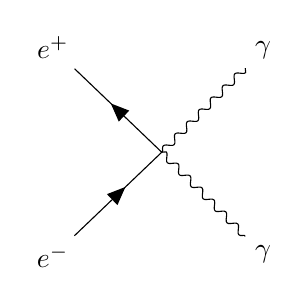
\begin{tikzpicture}
\begin{feynman}
\vertex (c) ;
\vertex [below left =of c] (i1){\(e^{-}\)};
\vertex [above left=of c] (i2) {\(e^{+}\)};
\vertex [below right=of c] (f1){\(\gamma\)};
\vertex [above right= of c] (f2){\(\gamma\)};
\diagram* {
(i1) -- [fermion] (c) -- [fermion] (i2) ,
(f1) -- [photon] (c)-- [photon] (f2)
};
\end{feynman}
\end{tikzpicture}
\caption{Electron-Positron Annihilation}
\label{Fey:e-p}
\end{center}
\end{figure}

\indent The weak interaction defines the interaction of particles under the weak isospin quantum number. There are two copies of each of every fermion, a left and a right-handed chirality version. Particle with a right-handed chirality have a weak isospin T = 0. These particles exist as singlets and do not interact with the weak force. Left-handed particles have a weak isospin T =  ${\frac{1}{2}}$. These particles live as doublets as illustrated in table ~\ref{tab:chiral}. For these particles, the third component of the weak isospin T\textsubscript{3}, ${+\frac{1}{2}}$ for up-type quarks and charged leptons and ${-\frac{1}{2}}$ for down-type quarks and neutral leptons. Under weak interactions, particles with ${T_{3} = +\frac{1}{2}}$ always transform into particles with ${T_{3} = -\frac{1}{2}}$, or vice versa.\linebreak

\begin{table}[h]
\begin{center}
\def\arraystretch{1.5}
\begin{tabular}[h]{|c|c|}
\hline
Left Handed Fermions, ${T = \frac{1}{2}, T_{3} = \pm\frac{1}{2}}$ & Right Handed Fermions, ${T = 0, T_{3} = 0}$\\
\hline\hline
${\binom{u}{d}}$, ${\binom{c}{s}}$, ${\binom{t}{b}}$, ${\binom{e}{\nu_{e}}}$, ${\binom{\mu}{\nu_{\mu}}}$, ${\binom{\tau}{\nu_{\tau}}}$ & u, d, c, s, t, b, e, ${\nu_{e}}$, ${\mu}$, ${\nu_{\mu}}$, ${\tau}$, ${\nu_{\tau}}$ \\
\hline
\end{tabular}
\caption{Particles of the Standard Model (ref XXX (ian or PDG))}
\label{tab:chiral}
\end{center}
\end{table}


 \indent The remaining piece of the weak interaction is the W boson. The W has an isospin of T = 1. This gives three option for the third component of isospin, ${T_{3} = +1, 0, -1}$ which give the W\textsuperscript{+}, the W\textsuperscript{0}, and the W\textsuperscript{-}. W\textsuperscript{0} will be discussed more in ~\ref{ssec:Higgs}. The ${W^{\pm}}$ either raise or lower the ${T_{3}}$ of the fermions. ~\ref{Fig:weak_dia} is an example of a weak interaction.\linebreak

\begin{figure}[h]
\begin{center}

\begin{tikzpicture}
\begin{feynman}
\vertex (i1){\(e^{-}\)};
\vertex [right =of i1] (c);
\vertex [right=of c] (f1) {\(\nu_{e}\)};
\vertex [below right=of c] (f2){\(W^{-}\)};
\diagram* {
(i1) -- [fermion] (c),
(f2) -- [boson] (c)-- [fermion] (f1)
};
\end{feynman}
\end{tikzpicture}
\caption{electron emitting an electron neutrino and a W Boson}
\label{Fig:weak_dia}
\end{center}
\end{figure}

%Here, write about mixing and electroweak interaction?
%Also need to talk briefly about QCD
%Need to talk about b-quarks specifically.

%\begin{equation}
%Y_{W} = 2(Q - T_{3})
%\end{equation}


\indent %Need to talk about couplings and decays more in depth here
\subsection{The Higgs Mechanism and Higgs Boson}
\label{ssec:Higgs}
%Start with need massless gauge bosons to fufill local gauge invariance. So we have W 1,2,3, and b. explain the mixing and the  break the symmetry to give the W+- Z and photon. Give math to explain this?? Show how this gives rise to a new boson, the higgs. 
QED is a gauge invariant theory. This means the Lagrangian that describes the system is invariant under local gauge transformations. For the electroweak theory, this is the electroweak symmetry. To satisfy this symmetry, the bosons must be massless. However, the electroweak bosons in the standard model, the ${W^{\pm}}$ the ${Z}$ and the ${\gamma}$ are not all massless. This means that the electroweak symmetry must be broken by something.\linebreak

\begin{figure}[h]
\begin{center}
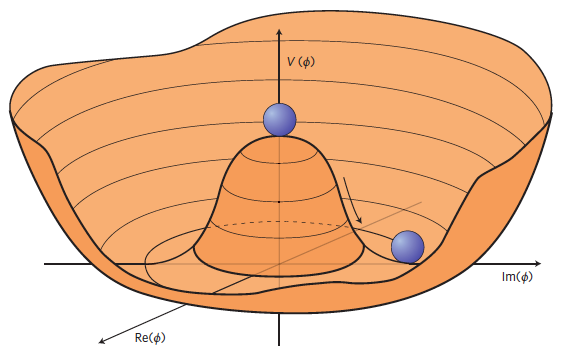
\includegraphics[scale=0.65]{figures/higgspotential}
\caption{The Higgs potential (from http://cds.cern.ch/record/1638469/plots) }
\label{Fig:higgspot}
\end{center}
\end{figure}

\indent In QED, the five gauge bosons are ${W^{i}_{\mu}, i = 1,2,3}$ and ${B_{\mu}}$. These bosons couple to a complex scalar Higgs doublet, ${\Phi \equiv \binom{\phi^{+}}{\phi^{0}}}$. This doublet has a scalar potential.
\begin{equation}
V(\Phi) = \mu^{2}|\Phi^{\dagger}\Phi| + \lambda(|\Phi^{\dagger}\Phi|)^{2}
\end{equation}
Where ${\mu^{2} < 0}$. This gives the Mexican hat shaped potential seen in figure ~\ref{Fig:higgspot}, with a minimum energy at 
\begin{equation}
\langle \phi \rangle = \sqrt{-\frac{\mu^{2}}{2\lambda}}\equiv \frac{\nu}{\sqrt{2}}
\end{equation}
called the vacuum expectation value (VEV) of ${\phi}$. The choice of the direction of fluctuation is arbitrary but can be chosen such that


 
\begin{equation}
\phi_{0} = \frac{1}{\sqrt{2}} \binom{0}{\nu}
\end{equation}
After the direction is chosen and the only remaining piece is the scalar field h(x), giving 
\begin{equation}
\phi(x) = \phi_{0} + h(x)
\end{equation}
The doublet can now be described by 
\begin{equation}
\Phi = \frac{1}{sqrt{2}} \binom{0}{v+h(x)}
\end{equation}
The Higgs field couples to the gauge bosons as 
\begin{equation}
(\frac{g}{2}\overrightarrow{\tau}\cdot \overrightarrow{W} + \frac{g'}{2}B)\phi_{0}
\end{equation}
Where ${\overrightarrow{\tau}}$ are the Pauli matrices, ${\overrightarrow{W}}$ are ${W_{1,2,3}}$ and g, g' are the coupling constants. The result of the coupling is the acquisition of mass by three eigenstates of the bosons, 
\begin{equation}
\begin{split}
W^{\pm} = \frac{1}{\sqrt{2}}(W^{1}_{\mu} \mp iW^{2}_{\mu})\\
Z^{\mu} = \frac{-g'B_{\mu} + gW^{3}_{\mu}}{\sqrt{g^{2} + g'^{2}}}\\
A^{\mu} = \frac{gB_{\mu} + g'W^{3}_{\mu}}{\sqrt{g^{2} + g'^{2}}}
\end{split}
\end{equation}
These four eigenstates are the bosons we observe in the standard model. With Masses
\begin{equation}
\begin{split}
M^{2}_{W} = \frac{1}{4}g^{2}\nu^{2} \\
M^{2}_{Z} = \frac{1}{4}(g^{2} + g'^{2})\nu^{2} \\
M_{A} = 0
\end{split}
\end{equation}
Through the mixing that occurs in the spontaneous electroweak symmetry breaking gives mass to the standard model Gauge Bosons while leaving the photon massless. However, for this to occur, an additional scalar field, the Higgs Field, is required.\linebreak
\indent The Higgs Boson is an excitation in the scalar Higgs field predicted in 1964. The decay mechanism of this massive boson was predicted by Peter Higgs, allowing for the decay products to be measured. Giving a way to prove the existence of the scalar Higgs field. In 2012, a Higgs like scalar boson was discovered at the LHC by the ATLAS and CMS experiments with a mass of 125GeV/c\textsuperscript{2} (ref XXX https://arxiv.org/abs/1207.7214). Since the discovery, many measurements have been made of this Higgs Boson to compare it to the standard model Higgs Boson. So far, the Higgs Boson has held up to these tests. The Higgs Boson has spin-parity J\textsuperscript{P} = 0\textsuperscript{+} 
(ref XXX %https://www.sciencedirect.com/science/article/pii/S0370269313006527?via%3Dihub)
, decays to bb (https://www.sciencedirect.com/science/article/pii/S0370269318307056), ${\gamma\gamma, \tau\tau}$,(ref XXX https://arxiv.org/abs/1811.08856) WW and ZZ have been measured with appropriate signal strengths, and no significant deviations have been observed in any Run 2 analyses. However, there are still many parameters of the Higgs Boson that still need measured. One of which is the triple Higgs coupling.
%Do I want to include more about the higgs discovery. 

%%%%%Use this as a filler to get the template working
%%Introduction
\chapter{Di-Higgs Production}
\label{chap:dihiggs}
Measuring di-Higgs production is necessary to further confirm the SM or find evidence for beyond the SM physics. The small SM production rate makes the channel an important place to look for new physics.  In particular, the di-Higgs production rate gives a handle to more accurately measure the Higgs potential.  This dissertation looks at both the measurement of the SM di-Higgs production rate and to search for new physics through resonant di-Higgs production. 
\section{Standard Model}
The Higgs self coupling potential in the SM is
\begin{equation}
V_{\mathrm{self-coupling}} = \lambda(|\Phi^{\dagger}\Phi|)^{2}
\end{equation}
When ${\Phi}$ is expanded around the VeV, $v$, the self coupling term can be written as
\begin{equation}
V_{\mathrm{self-coupling}} \supset \lambda v H^{3} + \frac{\lambda}{4}H^{4}
\end{equation}
where the first term, ${\lambda v H^{3}}$ is the coupling between three Higgs bosons with strength ${\lambda v \equiv \lambda_{HHH}}$\cite{Belusevic:2004pz}. The trilinear Higgs coupling can be probed at the LHC by measuring the cross section of events with two Higgs Bosons in the final state.\newline



\indent  Currently at the LHC, there are two dominant ways to produce di-Higgs events, the trilinear Higgs coupling gluon-gluon fusion (ggF) diagram and a box diagram, figure ~\ref{fig:dihiggs}. These diagrams interfere destructively, resulting in a SM prediction for the cross section, 
\begin{equation}
\sigma_{\mathrm{HH}} = 33.53\mathrm{fb}^{+4.3\%}_{-6.0\%}(\mathrm{QCD \ unc.})\pm{5.9\%} \mathrm{(other \ unc.)} 
\end{equation}
in pp collisions at 13 TeV \cite{Sirunyan:2018two}. This makes the trilinear coupling extremely hard to measure at the LHC. Additionally, since the cross section is so small, it is an promising place to look for deviations from the SM, since any enhancement to the cross section would be indicative of new physics.

\begin{figure}[h]
\footnotesize
\begin{center}
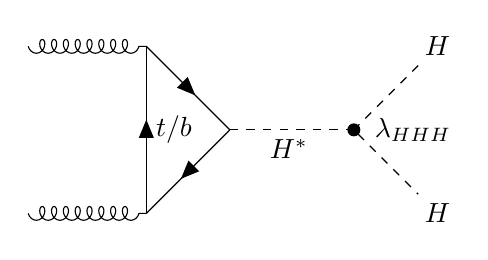
\begin{tikzpicture}
\begin{feynman}
\vertex (i1);
\vertex [right = of i1] (t1);
\vertex [dot][below right =of t1] (t3);
\vertex [below left= of t3] (t2);
\vertex [left = of t2] (i2);
\vertex [right =of t3][dot](h){};
\vertex [above right = of h] (f1){\(H\)};
\vertex [below right = of h] (f2){\(H\)};
\diagram* {
(i1) -- [gluon] (t1),
(i2) -- [gluon] (t2),
(t1) -- [fermion](t3) -- [fermion] (t2) -- [fermion,edge label'=\(t/b\)](t1),
(t3) -- [scalar,edge label'=\(H^{*}\)] (h),
(f1) -- [scalar] (h) -- [scalar](f2)
};
\vertex [right=0.75cm of h] {\(\lambda_{HHH}\)};
\end{feynman}
\end{tikzpicture}
\hspace{1cm}
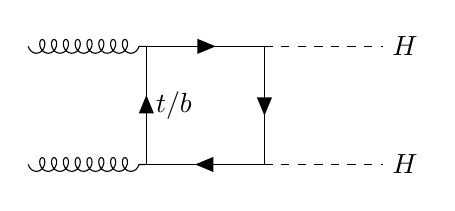
\begin{tikzpicture}
\begin{feynman}
\vertex (i1);
\vertex [ right = of i1] (t1);
\vertex [right = of t1] (t2);
\vertex [below = of t2] (t3);
\vertex [left = of t3] (t4);
\vertex [ left=of t4] (i2);
\vertex [ right =of t2] (f1){\(H\)};
\vertex [ right=of t3] (f2){\(H\)};
\diagram* {
(i1) -- [gluon] (t1),
(i2) -- [gluon] (t4),
(t1) -- [fermion](t2) -- [fermion] (t3) -- [fermion](t4) -- [fermion,edge label'=\(t/b\)] (t1),
(t2) -- [scalar] (f1),
(t3) -- [scalar] (f2)
};
\end{feynman}
\end{tikzpicture}
\caption[Di-Higgs production diagrams]{The dominate production method for di-Higgs events at the LHC with ${\sqrt{s} = 13 \text{ TeV}}$, with the trilinear Higgs coupling on the left}
\end{center}
\end{figure}
\label{fig:dihiggs}

\indent The SM di-Higgs production is a continuum production, with a turn-on at two times the Higgs mass, 250 GeV. Figure ~\ref{fig:SM_cont} shows the continuum distribution, as expected, it is a falling power law distribution peaked around 400 GeV. 

\begin{figure}[h]
\begin{center}
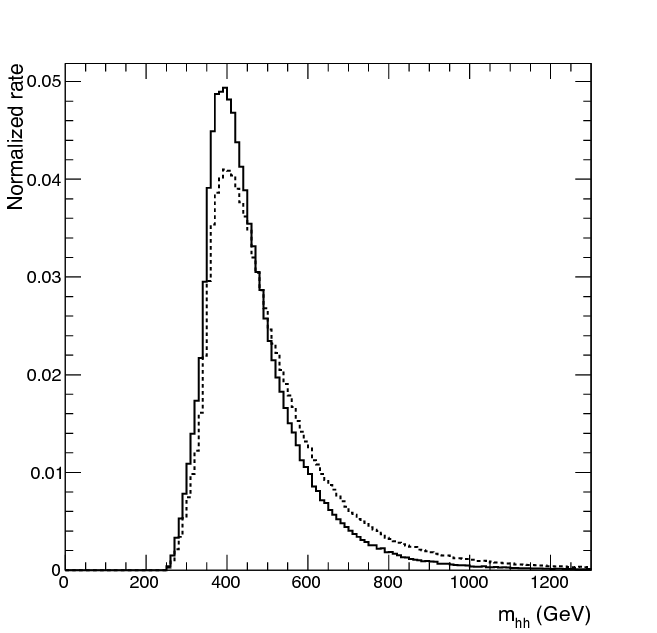
\includegraphics[scale=0.3]{figures/SM_continuum}
\caption[Normalized di-Higgs cross section]{Normalized differential cross section for pp ${\rightarrow}$ hh in the SM as a function of the invariant mass of the two Higgs bosons. The solid and dotted lines correspond respectively to ${\sqrt{s} = 14 \text{ and } 100 \text{ TeV}}$ .\cite{azatov:2015}}
\label{fig:SM_cont}
\end{center}
\end{figure}


\section{Resonant Production}
There are several BSM models that may enhance the rate of di-Higgs production at the LHC. This section will give an overview of a few of these models
\subsection{Complex Higgs Singlet}
The addition of a complex scalar singlet to the SM results in three neutral scalar particles after spontaneous symmetry breaking, which mix to give mass eigenstates, including the observed 125 GeV scalar \cite{PhysRevD.97.015022}.\newline
The normalizable scalar potential is
\begin{equation}
\begin{split}
V(\Phi,S_{c}) = \frac{\mu^{2}}{2}\Phi^{\dagger}\Phi + \frac{\lambda}{4}(\Phi^{\dagger}\Phi)^{2} \\
+ (\frac{1}{4}\delta_{1}\Phi^{\dagger}\Phi{}S_{c} + \frac{1}{4}\delta_{3}\Phi^{\dagger}\Phi{}S_{c}^{2} \\
+ a_{1}S_{c} + \frac{1}{4}b_{1}S_{c}^{2} + \frac{1}{6}e_{1}S_{c}^{3} + \frac{1}{6}e_{2}S_{c}|S_{c}|^{2} \\
+ \frac{1}{8}d_{1}S^{4} + \frac{1}{8}d_{3}S_{c}^{2}|S_{c}|^{2} + \mathrm{H.C.}) \\
+ \frac{1}{4}d_{2}(|S_{2}|^{2})^{2} + \frac{\delta_{2}}{2}\Phi^{\dagger}\Phi|S_{c}|^{2} + \frac{1}{2}b_{2}|S_{c}|^{2}
\end{split}
\end{equation}
\indent After spontaneous symmetry breaking, the fields are defined as:
\begin{equation}
\Phi = \binom{0}{\frac{h+v}{\sqrt{2}}}; S_{c} = \frac{1}{\sqrt{2}}(S+v_{s} + i(A + v_{A})).
\end{equation}
$v_{A}$ is set to 0 to conserve CP symmetry.\newline
The mass eigenstate fields are given by:
\begin{equation}
\begin{pmatrix}
h_{1}\\
h_{2}\\
h_{3}
\end{pmatrix}
= \begin{pmatrix}
c_{1} & -s_{1} & 0\\
s_{1}c_{2} & c_{1}c_{2} & s_{2}\\
s_{1}s_{2} & c_{1}s_{2} & -c_{2}
\end{pmatrix} 
\begin{pmatrix}
h\\
S\\
A\\
\end{pmatrix}
\end{equation}
where ${c_{i} = \cos{\theta_{i}}}$, h is the SU(2) doublet field, and S and A are the real and imaginary components of the complex scalar ${S_{c}}$.
Assigning the SM-like Higgs boson as ${h_{1}}$ with ${m_{1} = 125 GeV}$  and ${v = 246 GeV}$,  ${h_{2}}$ and ${h_{3}}$ are physical heavy Higgs bosons with ${m_{2}, m_{3} > m_{1}}$. The coupling of ${h_{1}}$ to SM particles is dominant, suppressed by a factor of ${c_{1}}$ from the SM rate, with the ${h_{2}}$ couplings suppressed by ${s_{1}c_{2}}$ and ${h_{3}}$ couplings suppressed by ${s_{1}s_{2}}$. ATLAS has set limits on ${c_{1} > 0.94}$ at 95\% CL in RUN-1. As the ${h_{1}}$ couplings become more SM-like (${\theta_{1}\rightarrow{0}}$), the allowed ${h_{2}}$ couplings become suppressed.\newline

\begin{figure}[h]
\begin{center}
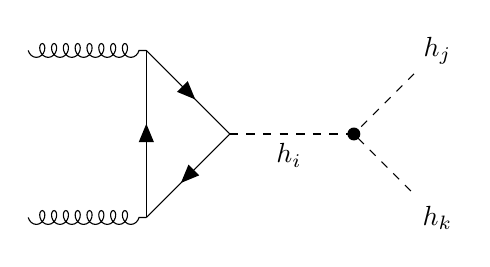
\begin{tikzpicture}
\begin{feynman}
\vertex (i1);
\vertex [right = of i1] (t1);
\vertex [dot][below right =of t1] (t3);
\vertex [below left= of t3] (t2);
\vertex [left = of t2] (i2);
\vertex [right =of t3][dot](h){};
\vertex [above right = of h] (f1){\(h_{j}\)};
\vertex [below right = of h] (f2){\(h_{k}\)};
\diagram* {
(i1) -- [gluon] (t1),
(i2) -- [gluon] (t2),
(t1) -- [fermion](t3) -- [fermion] (t2) -- [fermion](t1),
(t3) -- [scalar,edge label'=\(h_{i}\)] (h),
(f1) -- [scalar] (h) -- [scalar](f2)
};
\end{feynman}
\end{tikzpicture}
\hspace{1cm}
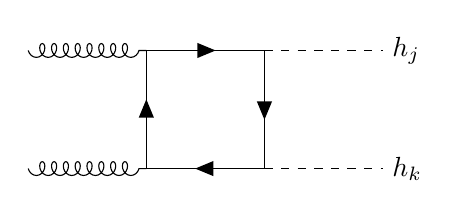
\begin{tikzpicture}
\begin{feynman}
\vertex (i1);
\vertex [ right = of i1] (t1);
\vertex [right = of t1] (t2);
\vertex [below = of t2] (t3);
\vertex [left = of t3] (t4);
\vertex [ left=of t4] (i2);
\vertex [ right =of t2] (f1){\(h_{j}\)};
\vertex [ right=of t3] (f2){\(h_{k}\)};
\diagram* {
(i1) -- [gluon] (t1),
(i2) -- [gluon] (t4),
(t1) -- [fermion](t2) -- [fermion] (t3) -- [fermion](t4) -- [fermion] (t1),
(t2) -- [scalar] (f1),
(t3) -- [scalar] (f2)
};
\end{feynman}
\end{tikzpicture}
\caption[BSM di-Higgs production diagrams]{Feynman diagrams for the production of ${h_{j}h_{k}}$, ${i, j, k = 1, 2, 3}$.}
\label{fig:FeyComp}
\end{center}
\end{figure}


\indent In the limit of ${\theta_{2}\rightarrow{0}}$, which is in agreement with the single Higgs rates, ${h_{3}}$ does not directly couple to SM fermions or vector bosons. The only way to produce ${h_{3}}$ is through ${h_{1}}$ or ${h_{2}}$, with the largest production rate from ${gg\rightarrow h_{2}\rightarrow h_{1}h_{3}}$, figure ~\ref{fig:FeyComp}. For a range of masses ${m_{2}}$ and ${m_{3}}$ the rate of production of ${h_{1}h_{3} \gg h_{1}h_{1}}$, figure ~\ref{fig:CSH6}. \newline

\begin{figure}[h]
\begin{center}
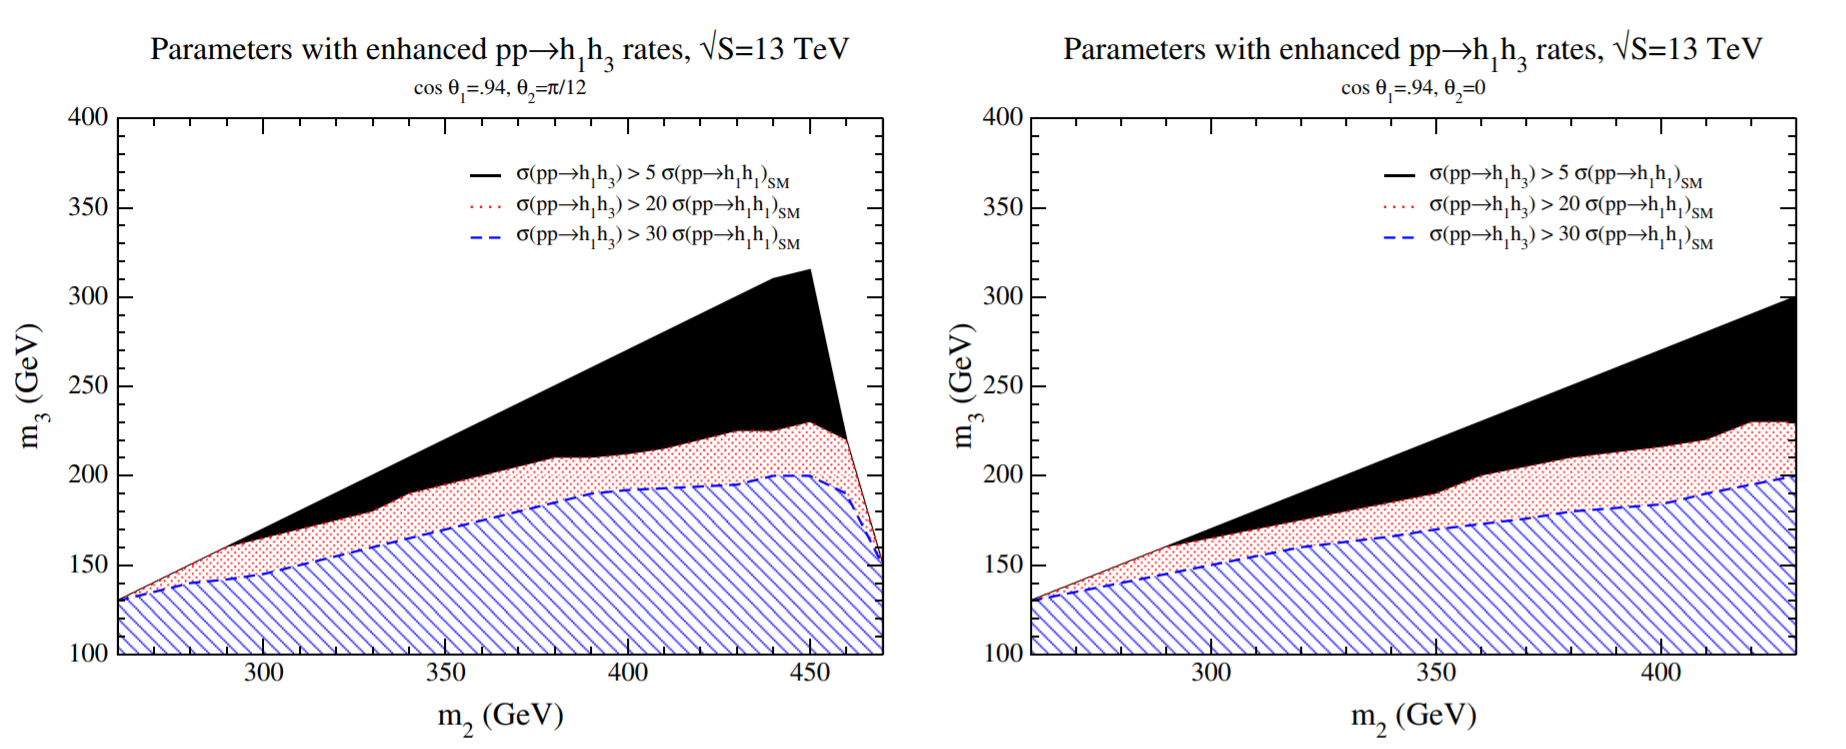
\includegraphics[scale=0.4]{figures/CompHiggsSing_Fig6_2}
\caption[Allowed regions of parameter space with enhanced di-Higgs production]{Regions of parameter space allowed by limits on oblique parameters $S$ $T$ and $U$ from Ref~\cite{deBlas2016}, perturbative unitarity of $2\rightarrow2$ scattering process \cite{PhysRevD.16.1519}, and the minimization of the potential where the rate for ${h_{1}h_{3}}$ production is significantly larger than the SM ${h_{1}h_{1}}$ rate at ${\sqrt{S} = 13 \text{ TeV}}$.}
\label{fig:CSH6}
\end{center}
\end{figure}


The enhancement can be see in the potential where 
\begin{equation}
V \rightarrow \frac{1}{2}\lambda_{211}h_{1}^{2}h_{2} + \frac{1}{2}\lambda_{311}h_{1}^{2}h_{3} + \frac{1}{2}\lambda_{331}h_{1}h_{3}^{2} + \frac{1}{2}\lambda_{321}h_{1}h_{2}h_{3} + . . .
\label{addhiggs}
\end{equation}
So while the SM trilinear Higgs coupling is determined by ${m_{h}}$, with this extension, the coupling is much less constrained. This leads to enhanced values seen in figure \ref{fig:CHS8}. So while this model would definitely show up in SM di-Higgs production, through the first two terms in equation ~\ref{addhiggs}, a search for one SM Higgs and a heavy Higgs would be more sensitive. This is a promising search moving forward but is not the focus of this dissertation.
\begin{figure}[h]
\begin{center}
\includegraphics[scale=0.65]{figures/CompHiggsSing_Fig8}
\caption[Allowed regions of parameter space with enhanced trilinear coupling]{Region of parameter space allowed by limits on oblique parameters, perturbative unitarity and the minimization of the potential where the ${h_{1}h_{1}h_{1}}$ trilinear coupling is greater than 5 times the SM value.}
\label{fig:CHS8}
\end{center}
\end{figure}

\subsection{Real Higgs Singlet Extension}
One simple explanation of an enhanced di-Higgs production rate at the LHC is the addition of a real scalar Higgs singlet, S \cite{Lewis:2017dme}. In this model, S can only interact with the SM through the Higgs field. In the case where there is no ${Z_{2}}$ symmetry, where ${S\rightarrow -S}$ the scalar field S mixes with the SM Higgs boson. If the mass is large enough, it is possible for S to decay to two on-shell SM Higgs Bosons, significantly enhancing the di-Higgs production rate.\newline
\indent The most general potential that can be added is 
\begin{equation}
V(\Phi,S) = -\mu^{2}\Phi^{\dagger}\Phi + \lambda(\Phi^{\dagger}\Phi)^{2} + \frac{a_{1}}{2}\Phi^{\dagger}\Phi S + \frac{a_{2}}{2}\Phi^{\dagger}\Phi S + b_{1}S + \frac{b_{2}}{2}S^{2} + \frac{b_{3}}{3}S^{3} + \frac{b_{4}}{4}S^{4}.
\end{equation}
Where $\Phi$ is ${\phi_{0} = \frac{(h + v)}{\sqrt{2}}}$ and ${<\phi_{0}> = \frac{v}{2}}$, while ${S = s + x}$ where ${x}$ is the vev of S. By shifting the field, it is possible the set ${x = 0}$. After electroweak symmetry breaking the fields mix to give the two mass eigenstates
\begin{equation}
\binom{h_{1}}{h_{2}} = 
\begin{pmatrix}
\cos{\theta} & \sin{\theta}\\
-\sin{\theta} & \cos{\theta}
\end{pmatrix}
\binom{h}{s}
\end{equation}
With ${m_{1} = 125 GeV}$, the free parameters are ${m_{2}, \theta,a_{2},b_{2}}$ and ${b_{4}}$. For di-Higgs production, in the case of ${m_{2}>2m_{1}}$, the important piece of the potential is 
\begin{equation}
V(h_{1}h_{2}) \supset \frac{\lambda_{111}}{3!}h_{1}^{3} + \frac{\lambda_{211}}{3!}h_{2}h_{1}^{2}
\end{equation}
This give an additional resonant double Higgs production diagram , figure ~\ref{fig:FeyRes}, for ${250 \text{ GeV } \leq m_{2}}$.
\begin{figure}[h]
\begin{center}
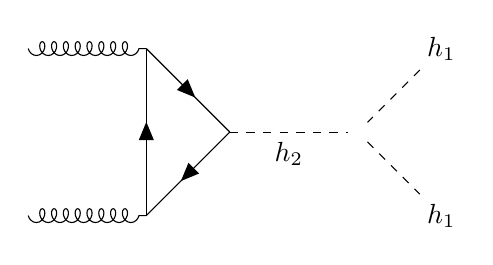
\begin{tikzpicture}
\begin{feynman}
\vertex (i1);
\vertex [right = of i1] (t1);
\vertex [dot][below right =of t1] (t3);
\vertex [below left= of t3] (t2);
\vertex [left = of t2] (i2);
\vertex [right =of t3](h){};
\vertex [above right = of h] (f1){\(h_{1}\)};
\vertex [below right = of h] (f2){\(h_{1}\)};
\diagram* {
(i1) -- [gluon] (t1),
(i2) -- [gluon] (t2),
(t1) -- [fermion](t3) -- [fermion] (t2) -- [fermion](t1),
(t3) -- [scalar,edge label'=\(h_{2}\)] (h),
(f1) -- [scalar] (h) -- [scalar](f2)
};
\end{feynman}
\end{tikzpicture}
\caption[Resonant di-Higgs production diagram]{Feynman diagram for ${h_{2}\rightarrow h_{1}h_{1}}$.}
\label{fig:FeyRes}
\end{center}
\end{figure}

\indent Varying the values of ${b_{4}}$ and ${\sin^{2}{\theta}}$, it is found that the maximum branching ratio (BR) for ${h_{2}\rightarrow h_{1}h_{1}}$ if obtained with ${b_{4} = 4.2, \sin^{2}\theta = 0.12}$. Figure ~\ref{fig:Ian6}, shows the minimum and maximum BR as a function of ${m_{2}}$. The largest BR is when ${m \approx 280 \text{ GeV}}$ at ${BR(h_{2}\rightarrow h_{1}h_{1}) = 0.76}$. This corresponds to an enhancement in di-Higgs production of approximately 30 times the SM cross section.

\begin{figure}[h]
\begin{center}
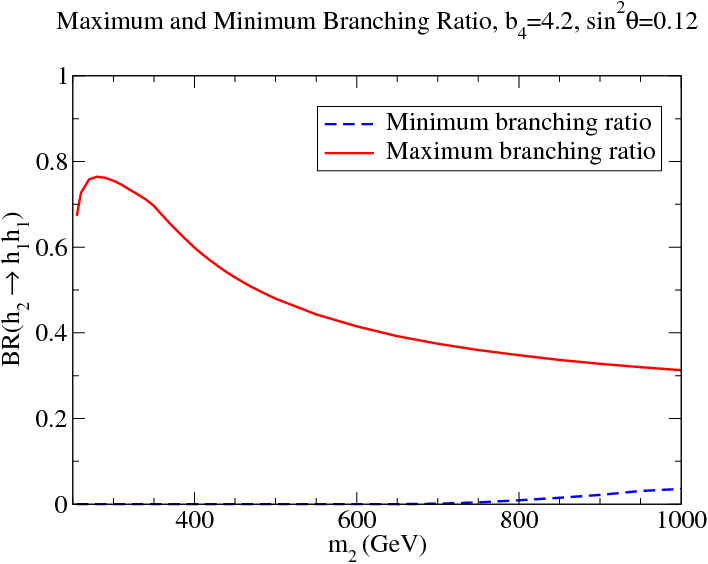
\includegraphics[scale=0.5]{figures/Ian6}
\caption[Allowed branching ratios for resonant di-Higgs production]{Maximum and minimum allowed ${BR(h_{2}\rightarrow h_{1}h_{1})}$ as a function of ${m_{2}}$ for ${b_{4} = 4.2}$ and ${\sin^{2}{\theta} = 0.12}$.}
\label{fig:Ian6}
\end{center}
\end{figure}

\section{Summary}
The SM di-Higgs production rate is an important and achievable measurement for the LHC and HL-LHC. It gives insight to the shape of the Higgs potential through measurement of the trilinear Higgs coupling. It is also a valuable discovery channel for BSM physics, especially for models with an extended Higgs sector, through resonant di-Higgs production. This dissertation will present results for both SM and resonant di-Higgs production.
%%%%%Use this as a filler to get the template working
%%Introduction
\chapter{Experimental Setup}
%ATLAS is a multipurpose detector positioned around one of the 4 primry interaction points of the Large Hadron Collider (LHC) in Geneva, Switzerland. The LHC collides protons at a center of mass energy of 13 TeV, for Run 2, at a rate of approximately 600MHz. 
\section{Hadronic Colliders}
Hadronic colliders use two beams of non-fundamental particles, typically proton-proton or proton-antiproton. These accelerators benefit from the larger mass of the particles when compared to lepton colliders. This results in smaller synchrotron radiation in circular accelerators, as the radiation is inversely proportional to mass. This allows hadronic colliders to have a much larger center of mass energy than leptonic colliders for the same size circular ring. \newline
\indent While hadronic colliders typically have larger collision energies, they also have significantly "messier" collisions. In leptonic colliders, the only final state particles come from the colliding particles. In hadronic colliders, not all of the constituents of the hadrons interact in the hard collision. This leads to many additional particles in the final state. Additionally, each subparticle only carries a portion of the hadron momentum, it is impossible to know the exact initial energy of the collision. 
\section{Overlapping Collisions}
\section{The Large Hadron Collider}
%Source
The Large Hadron Collider (LHC) is a 27 kilometer ring underneath the Franco-Swiss border. The LHC accelerates beams of protons (or ions) to a center of mass energy of up to 13 TeV(5 TeV) in two antiparallel beams around the ring. The particles are then collided at 4 primary interaction points each of which has a dedicated detector: ATLAS, CMS, ALICE, and LHCb.
\subsection{Detector Coordinates}
%Source
Within the ATLAS detector, the interaction point defined the origin of the coordinate system. The z-axis, the longitudinal axis, runs along the beam line, the positive x-axis points toward the center of the LHC ring, and the positive y-axis points toward the surface. The detector is also described in r, ${\eta}$, ${\phi}$ coordinates. With the transverse plane, the plane perpendicular to the beam line, being described by r and ${\phi}$. The radial coordinate, r, describes the distance from the beam line. The azimuthal angle, ${\phi}$, is the angle from the x-axis around the beam line. The final coordinate, ${\eta}$, is referred to pseudorapidity and is defined as ${\eta = -ln(tan(\frac{\theta}{2}))}$. With ${\theta}$ being the angle from the y-axis. The variable ${\Delta{R}=\sqrt{\eta^{2} + \phi^{2}}}$ is used to describe the distance between detector objects.
\section{Detector Overview}
%Source
\begin{figure}[h]
\begin{center}
\includegraphics*[width=0.60\textwidth] {figures/ATLAS_det}%Taken from http://iopscience.iop.org/article/10.1088/1748-0221/3/08/S08003/meta
\caption[The ATLAS detector]{The ATLAS detector}
\label{fig:ATLAS_det}
\end{center}
\end{figure}
The ATLAS detector, Figure~\ref{fig:ATLAS_det} is a general purpose detector and the largest on the LHC.  It is made up of concentric subsystems, each with a specialized task: the inner detector, which is responsible for measuring the charge and momentum of charged particles; the calorimeters, which are responsible for measuring the energy of different electromagnetic and hadronic particles; the muon spectrometer, which measures the momentum of minimum ionizing particles (MIP), like muons; and the magnet system, which is responsible for bending the charged particles in the detector, allowing their charge to be measured. The subdetectors feed into a vast Trigger and Data Acquisition (TDAQ) system that is responsible for selecting collision events with interesting characteristics.

\subsection{The Inner Detector}
%Source Inner detector TDR, I: https://cds.cern.ch/record/331063?ln=en
%Source Inner detector TDR, II: https://cds.cern.ch/record/331064?ln=en
%Source IBL TDR: https://cds.cern.ch/record/1291633?ln=en
\begin{figure}[h]
\begin{center}
\includegraphics*[width=0.60\textwidth] {figures/inner_3D}%Taken from ID TDR
\caption[Cross section of the Inner Detector.]{Cross section of the Inner Detector.}
\label{fig:ID_cs}
\end{center}
\end{figure}
%Tile: https://cds.cern.ch/record/2004868/files/ATL-TILECAL-PROC-2015-002.pdf
%Tile TDR: https://cds.cern.ch/record/331062?ln=en
%LAr TDR: https://cds.cern.ch/record/331061?ln=en
%LAr: https://www.physics.utoronto.ca/~krieger/procs/Krieger_NSS05_Proc.pdf
The inner detector (ID), Figure~\ref{fig:ID_cs}, is the closest system to the beam pipe. It contains 4 separate pieces. In order of distance from the beam pipe: The Insertable B-Layer (IBL), the Pixel Detectors, the Semiconductor Tracker (SCT), and the Transition Radiation Tracker (TRT). These subsystems work together to give charged particle tracking within the pseudorapidity range of ${|\eta| < 2.5}$. The inner detector is surrounded by a 2 T solenoid magnet, section ~\ref{ssec:mag}. The magnetic field causes charged particles to curve as they pass through the ID. The radius and direction of this curve give sign of the charge, positive or negative, along with a momentum measurement of the particle. The other task of the ID is vertexing, or determining if the transient particle came from the interaction point of a slightly displaced point. This is used to identify long lived particles, like bottom or charm quarks. This is discussed further in section ~\ref{ssec:btag}. \linebreak
\indent The IBL is the newest addition to the ID, being installed during the 2016 shutdown. It is place directly outside the beam pipe in order to maintain good vertexing and b tagging in increased pileup environments. In order to facilitate the insertion of the IBL, the beam pipe inner radius was decreased by 4 mm (from 29 mm to 25 mm). The IBL utilizes planar sensors, similar to the Pixel Detector, and 3D sensors, allowing electrons to interact to the bulk of the sensor as opposed to just the surface, and functions as a fourth pixel layer of the Pixel Detector.\linebreak
%Inner detector TDR Fig 3-1
\indent The Pixel Detectors are a network of high granularity, silicon pixels which measure the 2D position of passing charged particles. The silicon pixels are n-doped silicon wafers. A high voltage is applied to the wafer and when a charged particle passes through the silicon an electron hole pair is created. The electron drifts to the electrode and creates a signal that is read out by the electronics.  The Pixel detector barrel is divided into 3 cylindrical layers, the innermost layer is the B-layer, followed by Layer 1 and Layer 2. Each is covered in ${50\mu{m}}$ x ${300\mu{m}}$ silicon pixels. In order to ensure complete coverage, an end cap module is placed on each side of the barrel. The end-caps consist of 4 wheels, each with an inner and outer ring of trapezoid shaped silicon detectors. \linebreak
\indent The SCT is made of a barrel detector and two end-cap detectors. The barrel SCT has 4 cylindrical layers made up of pairs of 6.36 cm x 6.36 cm silicon crystals glued together along one side. The end-cap SCT tracker is made of rings of SCT modules with either silicon or galium arsenide. These rings are arranged into 9 wheels on each side of the barrel.\linebreak
\indent Outside of the silicon detectors lies the TRT. The TRT is a straw detector comprised of 50000, 4mm diameter straws in the barrel and 320000 radial straws in the end-caps. There are 420000 electronic channels, which give a spatial resolution of ${170\mu{m}}$ per straw. The straws are filled with various mixtures of xenon argon, carbon dioxide, tetrafluoromethane and nitrogen gas. When a charged particle passes through the TRT, they ionize the gas. The ionized gas is attracted to the oppositely charged straw and wire and produce a signal that is later amplified and read out. The xenon in the gas mixture allows for accurate particle identification from the transition radiation photon detection.  This gives a good discrimination between electrons and charged pions.

\subsection{Calorimeters}\label{ssec:calo}
%NOTE:::: Add general calo info
Outside of the solenoid magnet lies the calorimetry system. The calorimeters are responsible for measuring the energy of both charged and neutral particles, with the exception of MIPs and non-interacting particles such as neutrinos. The calorimeters can be broken into two distinct pieces, the liquid Argon calorimeter (LAr) and the tile calorimeter. \linebreak
\indent The Liquid Argon (LAr) calorimeter is a sampling calorimeter that is used for electromagnetic calorimetry for the entire range of acceptance (${|\eta{}|<4.8}$). It is also used for hadronic calorimetry for higher pseudorapidity ${1.4<|\eta{}|<4.8}$ In the central "barrel" of the calorimeter (${|\eta{}| < 1.4}$), is made up of 1024 lead-stainless-steel converters with copper-polyimde multilayer readout boards. The pates and readouts are arranged in an "accordion-shaped" geometry, Fig XXX. This allows for complete azimuthal coverage with no gaps, giving a constant electromagnetic energy resolution. In between the accordion layers, liquid argon is used as the active medium. The system is enclosed in a cryostat to maintain the temperature of the detector. The LAr barrel is divided radially into 4 sampling layers that are read out with a granularity of 0.1x0.1 ${\eta}$x${\phi}$ which are referred to as Trigger Towers. The granularity of the layers can be found in table XXXXX (LAR TDR table 1-2). The layer closest to the beamline is the Presampler. This layer sits inside of the cryostat and is responsible for  correcting for the energy loss in front of the calorimeter (the same is done in the endcap). Inside the cryostat, there are 3 additional layers, Fig XXXX. The thickness of the layers is often described in terms of radiation lengths ${\Xi_{0}}$. Where a radiation length is the distance a electron travels before it loses approximately 1/2 of it's energy to photon emission.  The front layer has a thickness of ${4.3\Xi_{0}}$, followed by the middle layer with a thickness of ${16\Xi_{0}}$ and the back layer of thickness ${2\Xi_{0}}$. Since the middle layer is the thickest, the bulk of the energy is absorbed in that layer. \linebreak 
\indent Forward from the barrel, there are two electromagnetic endcap (EMEC) wheels with a similar accordion structure to the barrel. One covering ${1.4 < |\eta{}| < 2.5}$ and one from ${2.5 < |\eta{}| < 3.2}$ Outside of the EMEC is the Hadronic endcap (HEC). This is also a copper-LAr sampling calorimeter. It has a simpler parallel plate design. Finishing out the LAr calorimeter is the Forward Calorimeter (FCal), which is contained in the endcap cryostat. This calorimeter is in the very forward region of the detector. In this region, the particle flux is very high, so a dense calorimeter is necessary to avoid energy leaking into other pieces of the detector. There are 3 layers in the FCAL, the first is made of copper and the other two are made of tungsten. They are matrices of metal with concentric tubes filled with Argon, see Fig XXXXX. TDR fig 1-9. \linebreak
\indent In the central region ${|\eta{}|<1.7}$, the tile calorimeter (TileCal) is responsible for the hadronic calorimetry. The TileCal is a sampling calorimeter with alternating iron plate absorbers and plastic scintillating tiles, the orientation can be seen in Fig XXXX (https://cds.cern.ch/record/2004868/files/ATL-TILECAL-PROC-2015-002.pdf, fig 2) . It has a fixed central barrel and 2 extended barrel sections that can be moved. The TileCal has a depth of ${7.4\lambda{}}$, where ${\lambda{}}$ is the nuclear interaction length, the mean distance a hadronic particle travels before it undergoes an inelastic interaction. The readout has the same granularity as the LAr trigger towers (0.1x0.1)
\subsection{Muon Detectors}
%Figure of muon cutaway: https://www.researchgate.net/figure/4-Cut-away-view-of-the-ATLAS-muon-system-from-Ref-3_fig10_254469099
%muon tdr: http://atlas.web.cern.ch/Atlas/GROUPS/MUON/TDR/pdf_final/mTDR.pdf
To detect muons, ATLAS uses four different technologies. For precision energy and position measurements, monitored drift tubes (MDT) and cathode strip chambers (CSC) are used. The CSCs are used in regions of high flux, where the MDTs are not suitable.  For the muon trigger system, a fast system is needed to keep up with the high collision rate of the LHC. In the central region, resistive plate chambers (RPC) are used, while in the forward region, where flux is higher, thin gap chambers (TGC) are used. The muon system, much like the ID utilize a magnetic field to determine the charge of passing particles. The magnet system is further discussed in Section~\ref{ssec:mag}.\linebreak
\indent The MDTs are made up of 6 parallel layers of cylindrical aluminum drift tubes with a tungsten-rhenium wires. The drift tubes are filled with a mixture of argon, nitrogen and methane. The tubes are assembled on a support of spacer and they are monitored for deformation by a built-in optical system, hence the \textbf{monitored} drift tubes. \linebreak
\indent While the MDTs are very good at precision measurements. However, they are not appropriate in areas whith the high rate counts (${> 200 Hz/cm^{2}}$) sue to their large diameter and high operating pressure. This is the case for the first layer of muon measurement with pseudorapidities of ${|\eta{}|>2.0}$. For this region, CSCs are the spectrometer of choice. CSCs are multiwire proportional chambers with a cathode strip readout. This gives good single and two track resolution in this high rate region.\linebreak
\indent In the barrel region, the muon trigger system employs RPCs, a low occupancy chamber with fast response. RPCs are gaseous parallel-plate detectors of Bakelite. The system can operate in two modes, avalanche and streamer.  In streamer mode, a large potential across the plates generates a discharge around the ionizing particle. For avalanche mode, a smaller potential difference and large signal amplification in the electornics allows for increased rate capability.\linebreak
%http://citeseerx.ist.psu.edu/viewdoc/download?doi=10.1.1.664.2817&rep=rep1&type=pdf
\indent Finally, in the end-cap of ATLAS, TGCs provide 2 important components. For the trigger system, TGCs have good timing resolution compared to the MDTs and can deal with a rate of up to 100 ${KHz/cm^{2}}$. For measurement, TGCs provide the azimuthal coordinate to compliment the bending coordinate from the MDTs. The TGCs are made up of anode wires and graphite cathodes in between layers of fiberglass laminate. 
\subsection{Magnet System}\label{ssec:mag}
%https://cds.cern.ch/record/338080?ln=en


\subsection{Trigger System}
\subsubsection{L1 Trigger}
\subsubsection{High Level Trigger}
\section{Simulation}





%%%%%Use this as a filler to get the template working
%%Introduction
\chapter{Simulation and Event Reconstruction}

\section{Simulation}
In order to draw conclusion from ATLAS data, it is necessary to compare to theoretical predictions. For particle collisions, it is not practical to create exact predictions, especially including detector effects such as resolution. To get the best estimate of these effects, ATLAS uses the Monte Carlo (MC) method to simulate data. This is done in multiple steps as illustrated by figure ~\ref{fig:eventsim}. \newline

\begin{figure}[h]
\begin{center}
\includegraphics*[width=0.70\textwidth] {figures/event_simulation}
\caption{Pictorial representation of how an event is generated \cite{Wanotayaroj:2242196}}
\label{fig:eventsim}
\end{center}
\end{figure}


\indent At the energies at the LHC, collisions usually do not involve entire protons. Instead, they involve constituents known as partons. Protons, while often described as two up quarks and a down quark, contain a sea of gluons. This sea of gluons also creates many virtual quark-antiquark pairs. The up and down quarks are the outer, or valance, quarks. These valance quarks are the primary role players in shallow inelastic interactions. At the LHC, the collision energies are sufficient for deep inelastic scattering, where the affects of the internal quarks and gluons are non-trivial. This internal structure of the proton is described  by a Parton Distribution Function (PDF), figure ~\ref{fig:pdf}. A PDF shows the probability density of finding a parton carrying a momentum fraction ${x}$ at a squared energy scale. %(http://www.scholarpedia.org/article/Introduction_to_Parton_Distribution_Functions)
\newline

\begin{figure}[h]
\begin{center}
\includegraphics*[width=0.65\textwidth] {figures/pdf.jpg}
\caption{The bands are ${x}$ times the unpolarized parton distributions
${f(x)}$ (where ${f = u_{v}, d_{v}, \bar{u}, \bar{d}, s \simeq{} \bar{s}, c = \bar{c}, b = \bar{b}, g}$) obtained in NNLO NNPDF3.0
global analysis at scales ${\mu^{2} = 10  GeV^{2}}$
(a) and ${\mu^{2} = 100  GeV^{2}}$ (b), with
${\alpha_{s}(M^{2}_{Z}) = 0.118}$.}
\label{fig:pdf}
\end{center}
\end{figure}


\indent The hard scattering process can be described using Feynman diagrams. These diagrams are a pictorial representation of amplitudes. These amplitudes go into calculating the matrix elements (ME) various interactions. In the event generation, these MEs are calculated to a specified order in perturbation theory. Common examples are leading order(LO), next-to-leading order(NLO) , and so on. The higher the order of the calculation, the more accurate the predictions. However, higher orders can be extremely hard to theoretically calculate. Often restricting the level of the event generator. \newline
\indent  After the ME generator, the hard partons are used as the inputs to the Parton Shower (PS) calculation. The PS calculation takes the hard scattering process from the event generator and calculates the parton shower. In addition to calculating the parton shower, the PS also calculates additional hard radiation processes not included in the base interaction. Colored particles can spontaneously emit gluons. These gluons, in turn, create either more gluons, or quark-antiquark pairs. This can happen either before (ISR) or after (FSR) the hard scattering process. Along with the ISR and FSR emittance, the PS generator can also describes the hadronization and subsequent decay of the hadrons into the final state particles. The precision of the PS generators are described similarly to the ME, with their contributions coming in as leading log (LL), next-to-leading-log (NLL), etc. for the parton showering process. \newline
\indent Finally, once the PS generator is complete, it is necessary to model the interactions of the final state particles as they pass through the ATLAS detector. ATLAS uses GEANT4  to handle this propagation\cite{geant4}. \newline
\indent The final result of the MC event generation is a set of simulated data that resembles actual data from the p-p collisions in the ATLAS detector. 
\section{Particle Identification}
For all events, either MC or actual collision data, it is important to be able to identify and reconstruct the underlying physics event. In particle collisions, the energy from the final state particles is deposited in the various subdetectors within ATLAS. These energy deposits must be translated to physically meaningful objects. This is the task of the event reconstruction, to use the ATLAS detector to recreate the final state particles for any given interaction. For this analysis, the final state particles present in the signal events are a lepton, either an electron or a muon; a neutrino, in the from of missing transverse energy; two light flavor quarks; and two b quarks. Each of these particles has a particular signal in each of the subdetectors, figure ~\ref{fig:crossSec}.

\begin{figure}[h]
\begin{center}
\includegraphics*[width=0.70\textwidth] {figures/layers}
\caption{Event Cross Section in a computer generated image of the ATLAS detector \cite{Pequenao:1096081}}
\label{fig:crossSec}
\end{center}
\end{figure}


\subsection{Electrons}
Electrons are reconstructed by fitting a track using the Inner Detector and matching this track to an energy cluster in the EM calorimeter\cite{Tarna:2286383}. As an electron passes through the EM calorimeter, it produces Bremsstahlung radiation photons. These photons then convert back to electron-positron pairs and the process repeats. This shower of electrons, positrons, and photons give the signature energy cluster in the calorimeter. Particles with the required Inner Detector track and matching EM energy cluster are selected as electron candidates.\newline
\indent Electron identification algorithms are applied to these electron candidates. These algorithms separate prompt, isolated electron candidates from backgrounds such as converted photons and misidentified jets. The electron identification algorithm is a multivariate likelihood discriminant using shower shape, track and track-to-cluster matching discriminating variables. There are three identification working points for electron identification: Loose, Medium, and Tight. Where the operating points wit higher background rejection are a subset of electron candidates with lower background rejection.\newline
\subsection{Muons}
The Muon Spectrometer specializes in muon detection and precision momentum measurement. Unsurprisingly, this makes the Muon Spectrometer (MS) a vital part of muon identification, but it is not the only subdetector used. The Inner Detector is also has an important part in reconstructing muons. In ATLAS, muon reconstruction is performed independently in the Inner Detector and the MS. The information is then combined to for the muon tracks. In the Inner Detector, the muons are reconstructed similarly to any other charged particle.\newline
\indent In the MS, the reconstruction looks for a hit pattern within each chamber to form segments \cite{Aad:2016jkr}. The MDT segments are combined using a straight-line fit. Segments in the CSCs are combined using a combinatorial search in the ${\eta}$ and ${\phi}$ planes. \newline
\indent Muon candidates are built by fitting together hits from segments in different layers. A combinatorial search, using segments in the middle layer as seeds, is performed. The inner and outer layers are then used as seeds as the search is extended. A minimum of 2 segments are required to build a track. It is possible for a segment to be included in multiple tracks, an overlap removal algorithm selects the best assigned track or can allow for a segment to be shared between two tracks. A global ${\chi^{2}}$ fit is performed on the hits of each track. If the ${\chi^{2}}$ of the fit passes a selection criteria, the track is accepted.\newline
\indent The information from the Inner Detector and the MS are then combined to give a muon signature. The combination method depends on the information available. The main method used is the Combined Muon reconstruction, where track reconstruction is performed in the Inner Detector and MS independently. Most of these muons are reconstructed using an ''outside-in" reconstruction. This  means tracks in the MS are extrapolated inward and matched to an Inner Detector track. \newline
\subsection{Jets}
Quarks very quickly undergo hadronization, with only the top quark decaying before hadronizing. This makes it impossible to measure a singular quark. Instead, collections of hadrons are formed and these are what deposit energy in the ATLAS detector. These collections of energy are called jets and can be made from various detector object. In this analysis in particular, two different types of jets are used: calo-jets, jets constructed from energy deposited in the calorimeters; and track-jets, jets constructed from tracks in the Inner Detector. \newline
\indent Since a jet is not a physical object, rather a collection of energy deposits, there are many ways to define a jet. Two important characteristics of any jet algorithm are Infrared (IR) Safety and Collinear (CL) Safety. For a jet algorithm to be IR Safe, the addition or subtraction of a soft jet will not change the jet collection. A jet algorithm is CL Safe if splitting or merging high transverse momentum particles does not change the jet collection. Figure \ref{fig:IR_CL} illustrates both IR and CL Safety.

\begin{figure}[h]
\begin{center}
\includegraphics*[width=0.70\textwidth] {figures/IR_CL_safe}
\caption{Illustration of the infrared sensitivity of a cursory designed jet algorithm (top). Illustration of the product of a collinear unsafe jet algorithm. A collinear splitting changes the number of jets (bottom). \cite{Isildak:2013kfa}.}
\label{fig:IR_CL}
\end{center}
\end{figure}

\indent Some examples of jet algorithms are visualized in figure ~\ref{fig:jetalgo}. For this analysis, the ${\textrm{anti-}k_{t}}$ algorithm is selected. In addition to being IR and CL safe, the ${\textrm{anti-}k_{t}}$ algorithm gives roughly circular jets. This makes calculating the energy density much easier than non-circular jets. The ${\textrm{anti-}k_{t}}$ algorithm has a radius parameter R. R acts as a cutoff radius for energy clustering and is not strictly a radius. The track-jets used in the analysis have R = 0.2, while the R = 0.4 and R = 1.0 calo-jets are used. \newline 

\begin{figure}[h]
\begin{center}
\includegraphics*[width=0.70\textwidth] {figures/jetalgo}
\caption{A sample parton-level event, together with many random soft
``ghosts", clustered with four different jets algorithms, illustrating the ``active" catchment areas of
the resulting hard jets\cite{Cacciari:2008gp}.}
\label{fig:jetalgo}
\end{center}
\end{figure}

\subsection{b Tagging}\label{ssec:btag}
B-Hadrons, composite particles that contain b quarks, travel a small distance before they decay. This means the track from the decay products can be traced back to the point at which the b-hadron decays, called the secondary, or displaced, vertex, figure ~\ref{fig:bjets} . This displaced vertex is used to tag jets that are likely to come from b quarks through b-tagging algorithms.\newline
\indent In this analysis, the MV2c10 is used to tag b-jets \cite{ATL-PHYS-PUB-2016-012}. MV2 is a multivariate discriminant that combines 3 b-tagging algorithms. The c10 signifies a 10\% c-jet fraction in the background training sample. The three algorithms that are used as inputs to the MV2 discriminant are: an impact parameter-based algorithm, an inclusive secondary vertex reconstruction algorithm, and a decay chain multi-vertex reconstruction algorithm. For this analysis, the 85\% fixed-cut working point is used for b-jet identification.\newline

\begin{figure}[h]
\begin{center}
\includegraphics*[width=0.70\textwidth] {figures/bjet}
\caption{Schmatic view of the tracks in a b-jet \cite{HanssonAdrian:1397942}.}
\label{fig:bjets}
\end{center}
\end{figure}

\subsection{Missing Transverse Momentum}
Neutrinos do not interact with the detector as they pass through. This means they cannot be measured like the other particles. In order to measure neutrinos, ATLAS relies on the conservation of momentum. As previously mentioned, the exact collision energy is unknown, as each partons does not carry a consistent fraction of the proton energy. However, in the transverse plane, the plane perpendicular to the beam line, the total momentum is known exactly. Before the collision, there is zero momentum in the transverse plane. After the collision, this must also be true. This implies the vector summation of all objects should have zero momentum in the transverse plane. Any imbalance in this is referred to as  Missing Transverse Momentum (\met). The \met{} is constructed as the negative vector sum of all reconstructed objects with an additional soft term reconstructed from detector signal objects not associated with any object\cite{ATL-PHYS-PUB-2015-027}. \newline
\indent The \met{} vector is a vector in the transverse plane, meaning it does not directly correspond to a neutrino. Additional information is needed to exactly reconstruct a neutrino. In this analysis, a Higgs mass constraint is used to supply the direction of the signal neutrino. \newline


%%%%%Use this as a filler to get the template working
%%Introduction
\chapter{Analysis}
\label{chap:anal}
This chapter will present the results of a search for Higgs boson pair production published in $JHEP$~\cite{Aaboud:2018zhh}. This chapter contains material coauthored with the ATLAS Collaboration. I developed the framework for the analysis, optimized the signal regions and developed the method for estimating QCD background. I was the primary contributor to the kinematic figures. Other members of the analysis group, members of the ATLAS Collaboration, estimated the other backgrounds that were used to produce the final result presented in this chapter. \newline
\indent In this analysis, one Higgs boson decays via ${H\rightarrow b\overline{b}}$ and the other via ${H\rightarrow WW^{*}}$ . The ${WW^{*}}$ system decays into ${l\nu qq}$ (where ${l}$ is either an electron or a muon). There is a contamination from the leptonic ${\tau}$ decays but it is small and not explicitly vetoed in the analysis. The Higgs boson decay modes chosen for this analysis are a compromise between signal efficiency and background rejection. The ${H\rightarrow WW^{*}}$ branching ratio of approximately 25\% is the second largest after ${H\rightarrow b\overline{b}}$ (approximately 58\%). The final state contains two b-quarks consistent with coming from one $H$, two light jets, an identified electron or muon plus \met{}, consistent with a $WW$ decay. The 1-lepton final state gives a strong discriminator against multijet background. The dominant backgrounds are \ttbar{} production, which has the same final state but with different kinematic properties; W bosons produced in association with jets (W+jets), where two of the associated jets come from b-quarks; and multijet events where a jet is misidentified as a lepton. There are smaller background contributions from single top-quark production, Z bosons produced in association with jets (Z+jets), and diboson production.\newline

\begin{figure}[h]
\begin{center}
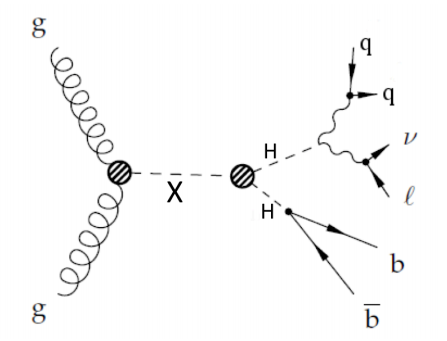
\includegraphics[scale=0.65]{figures/res_prod}
\caption[Schematic diagram of ${HH\rightarrow b\bar{b}WW^{*}\rightarrow b\bar{b}l\nu qq}$]{Schematic diagram of resonant Higgs boson pair production with the subsequent Higgs and W boson
decays.}
\label{fig:res}
\end{center}
\end{figure}

\indent This analysis sets limits on both SM Higgs boson pair production and on resonant production. Both production methods are discussed in detail in chapter \ref{chap:dihiggs}. Figure ~\ref{fig:res} shows a Feynman diagram of resonant production of the Higgs boson pairs with the subsequent decays ${H\rightarrow WW^{*}}$ and ${H\rightarrow b\overline{b}}$.

%%
\section{Analysis Overview}

Two complementary techniques are used to reconstruct the Higgs boson candidates that decays into two b-quarks\cite{Aaboud:2018zhh}. Both techniques use the ${\textrm{anti-}k_{t}}$ jet algorithm but with different radius parameters. The first technique uses jets with a radius parameter R = 0.4 and it is used when each b-quark from the ${H\rightarrow b\overline{b}}$ decay can be reconstructed as a distinct b-jet. This is referred to as the ``resolved analysis"\cite{DiMicco:2151893}. The second technique uses jets with a radius parameter R = 1.0, also know as fatjets, and is used when the b-quarks cannot be reconstructed as two distinct b-jets. Instead the Higgs boson candidate is identified as the single fatjet. This technique is referred to as the ``boosted analysis"\cite{Issever:2276099}. In both analyses, the jets from the hadronically decaying W boson are reconstructed as ${\textrm{anti-}k_{t}}$ jets with radius parameter R = 0.4. The non-resonant, SM production, search uses the resolved analysis exclusively, while the resonant analysis is performed using either the resolved or boosted analysis technique with the most sensitive technique chosen for each particular model and HH mass being tested.
\section{Data and Monte Carlo Samples}
\subsection{Data}
\indent The analysis presented uses the full proton-proton collision dataset collected in 2015 and 2016 as the center-of-mass energy of 13 TeV passing data quality checks requiring good conditions of all sub-detectors. The data that are currently used correspond to an integrated luminosity of 36.1 fb\textsuperscript{-1} (3.2 fb\textsuperscript{-1} from 2015 plus 32.8 fb\textsuperscript{-1} from 2016)\footnote{The following GoodRunLists (GRL) are used:\\  
data15\_13TeV.periodAllYear\_DetStatus-v79-repro20-02\_DQDefects-00-02-02\_PHYS\_StandardGRL\_All\_Good\_25ns.xml\\
and\\
data16\_13TeV.periodAllYear\_DetStatus-v88-pro20-21\_DQDefects-00-02-04\_PHYS\_StandardGRL\_All\_Good\_25ns.xml.\\
The GRLs were retrieved from the \href{https://twiki.cern.ch/twiki/bin/view/AtlasProtected/GoodRunListsForAnalysisRun2}{GoodRunListsForAnalysisRun2 twiki}}.

. 
\subsection{Monte Carlo Samples}
With the exception of the QCD multijet background described in~\ref{sec:multijet}, MC simulated events are used to estimate SM
backgrounds and the signal acceptances. Table~\ref{tabular:mc_samples} summarizes the MC samples
used for background estimation.

\begin{table}[!htb]
\begin{center}
\begin{tabular}{|l|c|c|}
  \hline
 Process & Generator       & $\sigma\times\text{BR}$ [pb]  \\ 
\hline

$t\bar{t} \to WWbb \to l \nu bb + X$ & \textsc{Powheg+Pythia6} & 451.65 \\
$Wt$~incl. & \textsc{Powheg+Pythia6} & 71.7 \\
single $t$,  s-channel, $\to l \nu + X$  & \textsc{Powheg+Pythia6} & 3.31 \\ 
single $t$,  t-channel, $\to l \nu + X$  & \textsc{Powheg+Pythia6} & 69.5 \\ 
$W$+jets, $W \to l \nu$ & \textsc{Sherpa} & 61510 \\
$Z$+jets, $Z \to l l$ & \textsc{Sherpa} & 6425  \\
Dibosons~incl. & \textsc{Sherpa} & 47.3 \\
$ggh~incl.$ & \textsc{Powheg+Pythia8} & 48.5 \\
$tth$, $\to l \nu + X$  & \textsc{aMC@NLO + Herwig++} & 0.223 \\
\hline
\end{tabular}
\caption{SM MC samples used for background estimation.}
\label{tabular:mc_samples}
\end{center}
\end{table}
The $t\bar{t}$ and single top-quark samples are generated
with \textsc{Powheg-Box} v2~\cite{Frixione:2007vw} using \textsc{CT10} parton distribution functions (PDF)
interfaced to \textsc{Pythia} 6.428~\cite{Sjostrand:2006za} for parton shower,
using the \textsc{Perugia2012}~\cite{Skands:2010ak} tune with
CTEQ6L1~\cite{Pumplin:2002vw} PDF for the underlying event descriptions.
\textsc{EvtGen} v1.2.0~\cite{Lange:2001uf} is used for properties of the bottomed
and charmed hadron decays. The mass of the top quark is set to $m_{t} =
172.5\,\GeV$. At least one top quark in the $t\bar{t}$ event is required to
decay to a final state with a lepton. The cross section of $t\bar{t}$ is 
known to NNLO in QCD
including re-summation of next-to-next-to-leading logarithmic (NNLL) soft gluon
terms, and the reference value used in ATLAS is calculated using \textsc{Top++}
2.0~\cite{Czakon:2011xx}. The parameter \textsc{Hdamp}, used to regulate the
high-\pt\ radiation in \textsc{Powheg}, is set to $m_{t}$ for good data/MC
agreement in the high \pt\ region~\cite{ATL-PHYS-PUB-2014-005}. Each process of
single top-quark ($t$-channel, $s$-channel and $Wt$-channel) is generated separately. The cross
section of single-top is calculated with the prescriptions in
Ref.~~\cite{Kidonakis:2011wy, Kidonakis:2010ux}. 

\textsc{Sherpa} v2.2.1~\cite{Gleisberg:2008ta} with the
\textsc{NNPDF 3.0}~\cite{Lai:2010vv} PDF set is used as the baseline
generator for the ($W \to \ell\nu$)/($Z\to \ell\ell$)+jets background.
The diboson processes ($WW$,
$WZ$ and $ZZ$) are generated with \textsc{Sherpa} with the \textsc{CT10} PDF
set.  

The $ggH$ and $VBF$ inclusive samples are generated with \textsc{Powheg} using
the \textsc{CT10} PDF set interfaced to \textsc{Pythia8} for parton
shower, while $ttH$ is a semi-leptonic sample generated with
\textsc{MADGRAPH5\_aMCAtNLO} interfaced to \textsc{Herwig++}. The ggF cross
section is normalised by using computations including up to three QCD
loops (N3LO \cite{Anastasiou:2016cez}. VBF, $Wh$ and $Zh$ samples,
  with inclusive $h$, $W$ and $Z$ decays
are also generated using \textsc{Pythia8}. 
%{\textbf under
%  generation...}


Signal samples are
generated with \textsc{MADGRAPH5\_aMCAtNLO}~\cite{Alwall:2014hca} interfaced to
\textsc{Herwig++} according to the procedure defined in Ref.~\cite{CP3Paper}. 
Events are generated with an effective
Lagrangian in the infinite top-quark mass approximation, and  reweighting the
generated events  with form factors that take into
account the finite mass of the top quark.  This procedure partially
accounts for the finite top-quark mass effects ~\cite{Degrassi_Ramona}. After the full analysis chain was developed, there were also developments in the theoretical front, which took full NLO calculation and top mass into account~\cite{Borowka:2016ypz, Borowka:2016ehy}. This led to a slight difference in $m_{HH}$ shape. A re-weighting scheme was then developed to correct $m_{HH}$ shape as described in these slides. {\footnote {https://indico.cern.ch/event/652372/}} The overall effect in the sensitivity is a loss of signal efficiency by about 30\%, which is also seen by other analysis such as $HH \rightarrow bbbb$. 

%Additional interpretation of the result is carried out in the context of bulk Randall-Sundrum (RS) model, which predict spin-2 Kaluza-Klein gravitons, $G_{KK}$~\cite{Agashe:2007zd, Fitzpatrick:2007qr}. Graviton signal samples are generated in the $G_{KK}\rightarrow HH \rightarrow bbWW$ channel. Events were generated at leading order with \textsc{MADGRAPH5\_aMCAtNLO v2.2.2}~\cite{Alwall:2014hca} using the \textsc{NNPDF 2.3} LO PDF set~\cite{Ball:2012cx}. The matrix elements were passed to  \textsc{Pythia 8.186}~\cite{Sjostrand:2007gs} for parton
%shower, hadronisation and simulation of the underlying event. The A14 set of tuned underlying event parameters~\cite{ATL-PHYS-PUB-2014-021} was used. The graviton signals were generated with $C = \kappa / M_{Pl} = 2.0$. For the interpretation of C = 1.0 case, the samples are then re-weighted as described in Ref.~\cite{Borowka:2016ypz, Borowka:2016ehy}.
 
Table~\ref{tabular:mc_samples_hh} shows the list of HH signals. 
%Two sets of samples are used. The 
%non-resonant signal sample use 
%SM production for the 
They use a heavy Higgs scalar model as the signal hypothesis. The 
masses of the heavy Higgs range from 260 GeV to 3000 GeV while
the Higgs width is set to$~10$ MeV, therefore the model is valid in
the Narrow Width Approximation (NWA).
The non resonnat signal is normalised to $\sigma {\rm (pp} \to {\rm  HH)} \times
{\rm Br(HH}\to{\rm  WWbb)} = 0.590$ pb, the resonant ones are
normalised to 0.044 pb for $m_H < 2000$~GeV and to 0.041 for $m_H \ge
2000$~GeV.

% The signals are normalised to the cross section upper limits from the Run1 ATLAS combined result~\cite{Aad:2015xja}. 



\begin{table}[!htb]
\begin{center}
\scriptsize
\begin{tabular}{|c|l|c|c|c|c|r|}
	\hline
 Process                                    & Generator    \\ \hline
HH SM & \textsc{MADGRAPH5\_aMCAtNLO} + Herwig++ including Form Factor \\
$H \to HH$ ($m_H =260 - 3000$) GeV & \textsc{MADGRAPH5\_aMCAtNLO} +
                                     Herwig++including Form Factor \\
\hline
\end{tabular}
\caption{Di-Higgs signal samples used in the analysis. }
\label{tabular:mc_samples_hh}
\end{center}
\end{table}


Additional pp collisions generated with \textsc{Pythia} 8.186 are
overlaid to model the effects of the pileup for all simulated
events. All simulated events are processed with the same
reconstruction algorithm used for data. All background samples are processed
through the full ATLAS detector simulation~\cite{Aad:2010ah} based 
on \textsc{GEANT4}~\cite{Agostinelli:2002hh} while signal samples use
the Atlas Fast simulation.

%%%
\section{Object Reconstruction}

The final state of this analysis includes electrons, muons, neutrinos and jets, including $b$-jets. 
The identification criteria and the selection applied to the reconstructed objects are defined in the
present section.

\subsection{Electrons}
\label{sec:el_def}

\subsubsection{Electron reconstruction}
\label{sec:el_reco}
%Electromagnetic (EM) clusters are reconstructed with a sliding window algorithm. EM clusters are associated with 
%a track refitted with GSF (Gaussian Sum Filter model)~\cite{ATLAS-CONF-2012-047} to account for bremsstrahlung energy losses. 
%%No vertex from conversion is required for the EM cluster of the electron candidate.
% 
%Electron identification is performed using a likelihood-based method. Variables used by the likelihood identification algorithm are the longitudinal 
%and transverse shower profiles, the track quality, the track and cluster positions to match in $\eta$ and $\phi$ and the presence 
%of high-threshold TRT hits. 
%The likelihood-based method includes most of the discriminating variables 
%that are difficult to use with explicit requirement without incurring significant efficiency loss. 



For this analysis, two set of electron selections are defined. They are denoted as VHLooseElectron and SignalElectron.
The selections are defined as the following

\textbf{VHLooseElectron}: The electron \pt~is required to be greater than 7 GeV. 
The electron cluster should be in the range of $|\eta|< 2.47$. 
Loose likelihood identification is applied in this criteria. 
Impact parameter significance ($|d_{0}^{\mathrm{sig}}| = d_{0}/\sigma{_{d_{0}}}$) less than 10 standard deviations. 
and $|\Delta{z_{0}^{\mathrm{IBL}}}\sin\theta| < 0.5$ mm are also required, where IBL refers to the ATLAS Insertable $B$-Layer. 

\textbf{SignalElectron}: The electron is required to pass the VHLooseElectron selection with its \pt~required to be greater than 27 GeV. 
The electron cluster should be in the range of $|\eta|< 2.47$ but excluded from the crack region ($1.37 < |\eta| < 1.52$).
Tight likelihood identification is applied in SignalElectron criteria with the impact parameter significance required to be 
less than 2. In addition, the electron is required to be isolated by passing the \texttt{FixedCutTightTrackOnly} 
isolation working point which corresponds to a cut on the ratio of ${p_{T}^{\mathrm{varcone0.2}}}$ to electron \pt of 0.06 (i.e ${p_{T}^{\mathrm{varcone0.2}}/ \pt < 0.06}$).

A summary of the electron selections is shown in Table~\ref{tab:electronsel}.

\begin{table}[htbp!]
\begin{adjustbox}{width=1\textwidth}
\centering
\begin{tabular}{ccccccc} \hline \hline
Electron Selection & \pt & $|\eta|$ & ID & $|d_{0}^{\mathrm{sig}}|$ &  $|\Delta{z_{0}^{\mathrm{IBL}}}\sin\theta|$ & Isolation \\ \hline
VHLoooseElectron   & $>$7~GeV  & $< 2.47$ & LH Loose & $ <10$ & $<0.5$ mm & - \\
SignalElectron     & $>$27~GeV & $< 2.47$ and $\notin [1.37, 1.52]$ & LH Tight & $  <2$ & $<0.5$ mm & \texttt{FixedCutTightTrackOnly} \\
\hline\hline
\end{tabular}
\end{adjustbox}
\caption{Electron selection requirements.}\label{tab:electronsel}
\end{table}

\subsection{Muons}
\label{sec:mu_def}
 
\subsubsection{Muon reconstruction}
\label{sec:mu_reco}
%Muon candidates are identified by using the algorithm described in
%Ref.~\cite{Muons2015}. Muons are selected within $|\eta| < 2.5$
%using track quality criteria based on the number of hits in the
%inner detector and in the muon spectrometer. Medium quality criteria 
%are used for muon identification. The criteria include muons
%identified in both the inner detector and muon spectrometer with
%good matching of the two tracks for $|\eta| < 2.5$.


For this analysis, two sets of muon selections are defined. They are denoted as VHLooseMuon and SignalMuon.
The selections are defined as the following:

\textbf{VHLooseMuon}: The muon \pt~is required to be greater than 7 GeV. 
The muon cluster should be in the range of $|\eta|< 2.7$. 
Loose identification is applied in this criteria. 
Impact parameter significance ($|d_{0}^{sig}|$) less than 6 standard deviations. 
and $|\Delta{z_{0}^{\mathrm{IBL}}}\sin\theta| < 0.5$ mm are also required. 

\textbf{SignalMuon}: The muon is required to pass the VHLooseMuon selection with its \pt~required to be greater than 27 GeV 
and should be in the range of $|\eta|< 2.4$. Medium identification is applied in SignalMuon criteria with the 
impact parameter significance required to be less than 2. In addition, the muon is required to be isolated by passing 
the \texttt{FixedCutTightTrackOnly} isolation working point which corresponds to a cut on the ratio of ${p_{T}^{mathrm{varcone0.3}}}$ to 
muon \pt of 0.06 (i.e ${p_{T}^{mathrm{varcone0.3}}/ \pt < 0.06}$).

A summary of the muon selections is shown in Table~\ref{tab:muonsel}.

\begin{table}[htbp!]
\begin{adjustbox}{width=1\textwidth}
\centering
\begin{tabular}{ccccccc} \hline \hline
Muon Selection & \pt & $|\eta|$ & ID & $|d_{0}^{\mathrm{sig}}|$ & $|\Delta{z_{0}^{\mathrm{IBL}}}\sin\theta|$ & Isolation \\ \hline
VHLoooseMuon   & $>$7 GeV  & $ < 2.7$ & Loose quality  & $ <6$ & $<0.5$ mm & - \\
SignalMuon     & $>$27 GeV & $ < 2.4$ & Medium quality & $ <2$ & $<0.5$ mm & \texttt{FixedCutTightTrackOnly} \\
\hline\hline
\end{tabular}
\end{adjustbox}
\caption{Muon selection requirements.}
\label{tab:muonsel}
\end{table}

\subsection{Jets}
\label{sec:jet_def}
\subsubsection{Large-R jets}
For signal processes with a large resonant mass the b-jets produced by the Higgs may be too close together
to be resolved by the R=0.4 calorimeter-based jets (calo-jets). This effect is expected to be noticeable when ${p_{T}^{H} > 500\mathrm{GeV}}$\footnote{Using the rule of thumb ${}\Delta R = 2m/\pt$, where ${m = m_{H}}$ and ${\Delta R = 0.4}$}.
Our approach to reconstructing the ${H\rightarrow b\overline{b}}$ system in this ``boosted" regime is to use a large radius (large-R) jet with radius parameter R =1.0. The large-R jets are required to have ${\pt > 250 \mathrm{GeV}}$ and ${|\eta| < 2.0}$.
\subsubsection{Track jets}
To identify a large-R jet that is consistent with decay of ${H\rightarrow b\overline{b}}$, a method developed by ATLAS is to reconstruct subjets within the large-R jet and identify the subjets whether it is a b-jet or not by using a b-tagging algorithm. The baseline method is to use subjets built from tracks (track jets).
For the boosted analysis, track jets are required to have ${\pt > 10 \mathrm{GeV}}$ and ${|\eta| < 2.5}$ for them to be within the inner detector acceptance. They are also required to have at least 2 track constituents. The MV2c10 working point for track jets is the 77\% Fixed Cut efficiency.

\subsubsection{Small-R jets}


\textbf{Signal jets} are defined as jets which passes the jet cleaning and JVT criteria, described in the previous section.
They are further required to have $\pt > 20$ GeV and $|\eta| < 2.5$.

%\newcommand{\BTagWPFootNote}{The charm quark component is suppressed by a factor 3.10 while the 
%light quark component is suppressed by a factor 33.5. The expected performance is documented 
%on the \href{https://twiki.cern.ch/twiki/bin/view/AtlasProtected/BTaggingBenchmarks\#MV2c10_tagger_added_on_11th_May}{BTaggingBenchmarks twiki}.}

%The ATLAS jet flavor tagging algorithm, here the \texttt{MV2c10} algorithm~\cite{ATL-PHYS-PUB-2016-012}, is used to select signal jets and suppress multi-jet, $W$+jets, $Z$+jets and di-boson background. 
%Out of the possible working points corresponding to different $b$-tagging efficiencies, the 85\% Fixed-Cut\footnote{\BTagWPFootNote} working point (WP) is selected as to keep the signal efficiency high. 
Signal jets are labeled \textbf{b-jets} if they pass the \texttt{MV2c10} 85\% WP cut and labeled as \textbf{light-jets} if they fail the cut.



Table~\ref{tab:sjdefinit} summarizes the jets selection. 

\begin{table}[htbp!]
\centering 
\small
\begin{tabular}{|c||c|}        
 \hline
 & Signal Jets\\
 \hline
 Algorithm            & anti$-k_t$\\
 $p_T$                & 20~GeV\\
 $|\eta|$             & $< 2.5 $\\
 Quality              & not ``bad'' jet\\
 Pile-up jet removal & JVT $> 0.59$ when $|\eta| < 2.5 ~ and ~p_T < 60 $ GeV\\    
 $b$-tagging          &  \texttt{MV2c10}, 85\% fixed-cut WP, labelled as b-jets pass cut, light-jets if fail cut\\ 
\hline                          
\end{tabular}
\caption{Selection for jets with distance parameter $R = 0.4$.}
\label{tab:sjdefinit}
\end{table}

\subsection{Missing transverse momentum ($\met$)}
\label{sec:met_def}

%The neutrino is not directly detectable and, thus, appears only as an imbalance in
%transverse momentum.
%\footnote{Transverse momentum is defined as the components of
%momentum in the plane perpendicular to the beam axis.}.
	
The missing transverse momentum (MET, or \met)~\cite{ATL-PHYS-PUB-2015-027} used in this analysis is computed by using electrons that pass the VHLooseElectron selection, muons passing the VHLooseMuon selection and jets of the analysis.\footnote{From MET\_Core\_AntiKt4EMTopo with the MissingETAssociationMap using the METMaker tool. All calibrated jets are passed to the METMaker tool as prescribed on the EtMiss subgroup \apkg{https://twiki.cern.ch/twiki/bin/view/AtlasProtected/EtmissSubgroup}{twiki}} The track-based soft term\footnote{Defined on this \href{https://twiki.cern.ch/twiki/bin/view/AtlasProtected/EtmissSubgroupTrackSoftTermDescription}{twiki}.} (TST) is the recommended soft term component for the MET calculation. Photons and hadronically decaying taus are included in the $\met$ calculation as jets since they are not used explicitly in the event reconstruction.

\subsection{Overlap removal}
\label{sec:overlapremoval}
In order to uniquely identify objects, overlapping objects are removed according to the overlap removal procedure defined in this section. 
Electrons and muons that pass the VHLooseElectron and VHLooseMuon selections (as defined in Sec.~\ref{sec:el_reco} and ~\ref{sec:mu_reco}) are considered for overlap removal. 
Calorimeter jets which pass the JVT requirement are also considered for overlap removal. The procedure is defined as follows.

If an electron and a muon shares a track, the muon is removed if it is \textit{calo-tagged}. Otherwise, the electron is removed.
Calorimeter jets are then removed if they are within $\Delta R(\text{calo-jet}, \text{electron})$ < 0.2 of surviving electrons. 
Electrons that satisfy $\Delta R(\text{electron},\text{calo-jet})$ < min(0.4, 0.04 + 10 \GeV /$E^\text{electron}_\text{T}$) are removed. 
The surviving calorimeter jets are removed if they are within $\Delta R(\text{calo-jet}, \text{muon})$ < 0.2 and 
do \textbf{not} pass any of the following criteria:

\begin{itemize}
\item The number of tracks in the jet are more than 2.
\item $\pt^{\text{muon}} / \pt^{\text{calo-jet}} < 0.5$  AND  $\pt^{\text{muon}} / \pt^{\text{tracks in calo-jet}} < 0.7$.
\end{itemize}

Muons that satisfy $\Delta R(\text{muon},\text{calo-jet})$ < min(0.4, 0.04 + 10 \GeV /$\pt^\text{muon}$) are removed. 
The overlap removal procedure is implemented using ASG's 
\apkg{https://svnweb.cern.ch/trac/atlasoff/browser/PhysicsAnalysis/AnalysisCommon/AssociationUtils/trunk/doc/README.rst}{AssociationUtils} 
package and summarized in Table~\ref{tab:overlapremoval}.

\begin{table}[htbp!]
\centering
\tiny
\begin{tabular}{l | l}
\toprule
Overlapping Objects & Removal Procedure \\
\midrule
Electron - Muon   & If share track, remove muon if calo-tagged. Otherwise remove electron.\\ 
\hline
\multirow{2}{*}{Electron - Calo-jet} & If $\Delta R(\text{calo-jet}, \text{electron})$ < 0.2, remove calo-jet.\\
& If $\Delta R(\text{electron},\text{calo-jet})$ < min(0.4, 0.04 + 10 \GeV /$E^\text{electron}_\text{T}$), remove electron.\\ 
\hline
\multirow{4}{*}{Muon - Calo-jet} & If $\Delta R(\text{calo-jet}, \text{muon})$ < 0.2, remove calo-jet if: \\
& a) Number of tracks in calo-jet $\leq$ 2, OR \\  
& b) $\pt^{\text{muon}} / \pt^{\text{calo-jet}} > 0.5$  AND  $\pt^{\text{muon}} / \pt^{\text{tracks in calo-jet}} > 0.7$.\\
& If $\Delta R(\text{muon},\text{calo-jet})$ < min(0.4, 0.04 + 10 \GeV /$\pt^\text{muon}$), remove muon.\\ 
\bottomrule
\end{tabular}
\caption{A summary of the overlap removal procedure.} 
\label{tab:overlapremoval}
\end{table}

%%%
\section{Resolved Analysis}
\label{sec:Resolved}

\subsection{Event Selection}
\label{sec:resolved_selection}
The final state of interest consists of one charged lepton, one neutrino, 
and four quarks, two of which are b-quarks. Hence the detector signature
consists of one  charged lepton ($e$/$\mu$), large $\met$, and four or more
anti-$k_t$ jets of which two are $b$ jets from the $h$ decay while the other
two are light jets from the hadronic decay of the $W$ boson. One challenge
in the event reconstruction is to correctly identify the pair of light jets
from the $W$ boson decay. This information is also used to solve the $z$
component of the neutrino momentum. For the HH signal there is an additional
complication due to the fact that one of the 
$W$ bosons is off-shell, and thus for this $W$ there is no $W$ mass constraint. 
This section details the stages of the event reconstruction and the
progression towards the final selection which defines the signal
region.  In addition, signal depleted control regions are defined in the
next section which are used to check the consistency of the SM background
predictions with the data in the control regions. The search
has been kept ``blinded'' until the comparison between data and
simulation of backgrounds are well understood in the signal depleted
control regions.

\subsection{Trigger requirement}

Events are selected using the unprescaled single lepton triggers. The list of triggers used in 
this analysis is shown in Table~\ref{tab:triggers}. Events are selected with a logical OR between 
the triggers listed in Table~\ref{tab:triggers}.

\begin{table}[htbp!]
\begin{center}
 \begin{tabular}{|c|c|}
  \hline
  Dataset & Trigger items \\
  \hline
  \multirow{2}{*}{2015} & mu20\_iloose\_L1MU15  \\
    & mu50  \\
    & e24\_lhmedium\_L1EM18VH (MC)  \\
    & e24\_lhmedium\_L1EM20VH (data)  \\
    & e60\_lhmedium  \\
    & e120\_lhloose  \\
  \hline
  \multirow{8}{*}{2016 - Period A} & mu24\_iloose\_L1MU15 (MC)  \\
    & mu24\_iloose (data)  \\
    & mu40  \\
    & e26\_lhtight\_nod0\_ivarloose  \\
    & e60\_lhmedium\_nod0  \\
    & e60\_medium  \\
    & e140\_lhloose\_nod0  \\
    & e300\_etcut  \\
  \hline
  \multirow{7}{*}{2016 - Period B-D3} & mu24\_ivarmedium  \\
    & mu50  \\
    & e26\_lhtight\_nod0\_ivarloose  \\
    & e60\_lhmedium\_nod0  \\
    & e60\_lhmedium  \\
    & e140\_lhloose\_nod0  \\
    & e300\_etcut  \\
  \hline
  \multirow{7}{*}{2016 - Period D4-E3} & mu26\_ivarmedium  \\
   & mu50  \\
   & e26\_lhtight\_nod0\_ivarloose  \\
   & e60\_lhmedium\_nod0  \\
   & e60\_lhmedium \\
   & e140\_lhloose\_nod0  \\
   & e300\_etcut  \\
  \hline
  \multirow{7}{*}{2016 - Period $\ge$ F} & mu26\_ivarmedium   \\
   & mu50  \\
   & e26\_lhtight\_nod0\_ivarloose  \\
   & e60\_lhmedium\_nod0  \\
   & e60\_lhmedium  \\
   & e140\_lhloose\_nod0  \\
   & e300\_etcut  \\
  \hline
 \end{tabular}
\end{center}
\caption[List of triggers used]{Summary of trigger items used for 2015 and 2016 data. For 2016 data, different triggers were used for different data run periods. 
All triggers are unprescaled.}
\label{tab:triggers}
\end{table}


\subsubsection{Pre-selection}
The following selection cuts are applied at the pre-selection level to the recorded events:
\begin{itemize}
\item In order to assure good data quality, events with bad detector
  conditions, namely where large part of the detectors were missing
  from data acquisition due to problems during a run, or when the
  performance of the detectors were affected by large noise, have been
  rejected from the data analysis. A GRL selection taken from
  data15\_13TeV.periodAllYear\_DetStatus-v79-repro20-02\_DQDefects-00-02-02\_PHYS\_StandardGRL\_All\_Good\_25ns.xml
  and data16\_13TeV.periodAllYear\_DetStatus-v88-pro20-21\_DQDefects-00-02-04\_PHYS \\ \_StandardGRL\_All\_Good\_25ns.xml
  is applied. Moreover, incomplete events or events with bad detector information are rejected. 
  \iffalse
  \footnote { {\small
\begin{verbatim}
  eventInfo->errorState(xAOD::EventInfo::EventFlagSubDet::Tile) == xAOD::EventInfo::Error,
  eventInfo->errorState(xAOD::EventInfo::EventFlagSubDet::LAr)  == xAOD::EventInfo::Error,
  eventInfo->errorState(xAOD::EventInfo::EventFlagSubDet::SCT)  == xAOD::EventInfo::Error, 
  (eventInfo->eventFlags(EventInfo::Core) \& 0x40000) is true.
\end{verbatim}
}
}
\fi

\item The presence of a  primary vertex with at least two
  tracks. Among all primary vertices, that with the highest
	$\sum p_{{\rm T,trk}}^{2}$, where
	$p_{{\rm T,trk}}$ is the transverse momentum of tracks
	associated with the vertex, is retained as the primary
  interaction vertex;
\item at least one SignalElectron ($e$) or SignalMuon ($\mu$), as defined in Sec.~\ref{sec:el_reco} and Sec.~\ref{sec:mu_reco}, and it must be trigger matched to the 
corresponding HLT object which fires the trigger;
\item at least 4 jets, of which 2 and only 2 are $b$-tagged.
\end{itemize}

\subsection{Event Reconstruction}
\label{ssec:event_reco_res} 
%%The final state of our signal consists of one charged lepton, one neutrino, and four quarks, 
%%two being $b$-quraks. Hence the detector signature consists of one charged lepton, missing 
%%transverse momentum, and four or more jets of which two are $b$ jets from the $h$ decay while 
%%the other two are light jets from the hadronic decay of the $W$ boson. 
Events are reconstructed by first requiring exactly two 2 $b$-tag jets and at least 2 light
jets and at most 3 light jets. In events with 3 light jets, the pair with the 
lowest $\Delta R$ between them are selected as $W$ jet candidates. This
procedure yields the correct jet assignment in 70\% of the cases for
signal events where the
hadronic daughters of the $W$ boson can be correctly matched to reconstructed
jets as described in Appendix~\ref{app:jetTruthStudies}.
%After preselection both light jets from $W$ bosons can be correctly matched in  20 \% of events.(see Appendix \ref{sec:BenStudy}).  

The event kinematics of the $H \to WW^* \to l \nu qq$ topology can be fully
reconstructed. In fact, among all four-momenta of the final state particle,
only the component of the neutrino momentum along the beam axis, $p_z$ in the following, is unknown while its transverse
momentum is the measured $\met$. Imposing the relation:
\begin{equation}
\label{eq:mh}
m_h^2 = (p^l + p^{\nu} + p^{j1} + p^{j2})^2
\end{equation}
where $p^i$ is the four-momenta of particle $i$, the neutrino $p_z$ can be
reconstructed using the relations:
\[
p_E^{\nu} = E^{\nu} = \sqrt{P_T^2 + p_z^2} \quad p_x^{\nu} = P_Tcos(\phi) \quad p_y^{\nu} = P_T sin(\phi)
\]
where $\phi$ is the azimuthal angle of the $\met$, $E^{\nu}$ the neutrino
energy, $p_x$ and $p_y$ the two transverse spatial components of the neutrino momentum.
Eq. \ref{eq:mh} is a quadratic expression in $p_z$. It can have two real,
one real  or two complex solutions. In the last case only the real part of the
complex solution is taken into account, therefore a single value of $p_z$ is
obtained. In the first case the solution with the neutrino direction closest
to the charged lepton is retained. It has been shown that this algorithm
selects the correct solution in approximately 60\% of the cases
(see Appendix~\ref{app:nupz_studies}).

\subsection{$bb\tau\tau$ analysis overlap removal}
In order to remove overlap with the $bb\tau \tau$ analysis we reject
any event containing at least one hadronic $\tau$ candidate that could be
identified by the $bb\tau\tau$ analysis, that fullfill the following
requirements:
\begin{itemize}
\item $p_T > 20$ GeV and $|\eta| < 2.5$;
\item one or three prongs;
\item unit charge;
\item pass the medium $\tau$ ID BDT working point.
\end{itemize}

The rejection of such events causes a signal efficiency drop of about 3\%.

\subsection{Kinematic selection}
\label{subsec:kincuts}


Kinematic selection is used to suppress mainly $t\bar{t}$ background while keeping
high signal efficiency.  A schematic view of the $HH \to WW{*}b\overline{b}$ and the
$t \bar{t} \to WWbb$ event topology is shown in Figure \ref{fig:cartoon}.
\begin{figure}
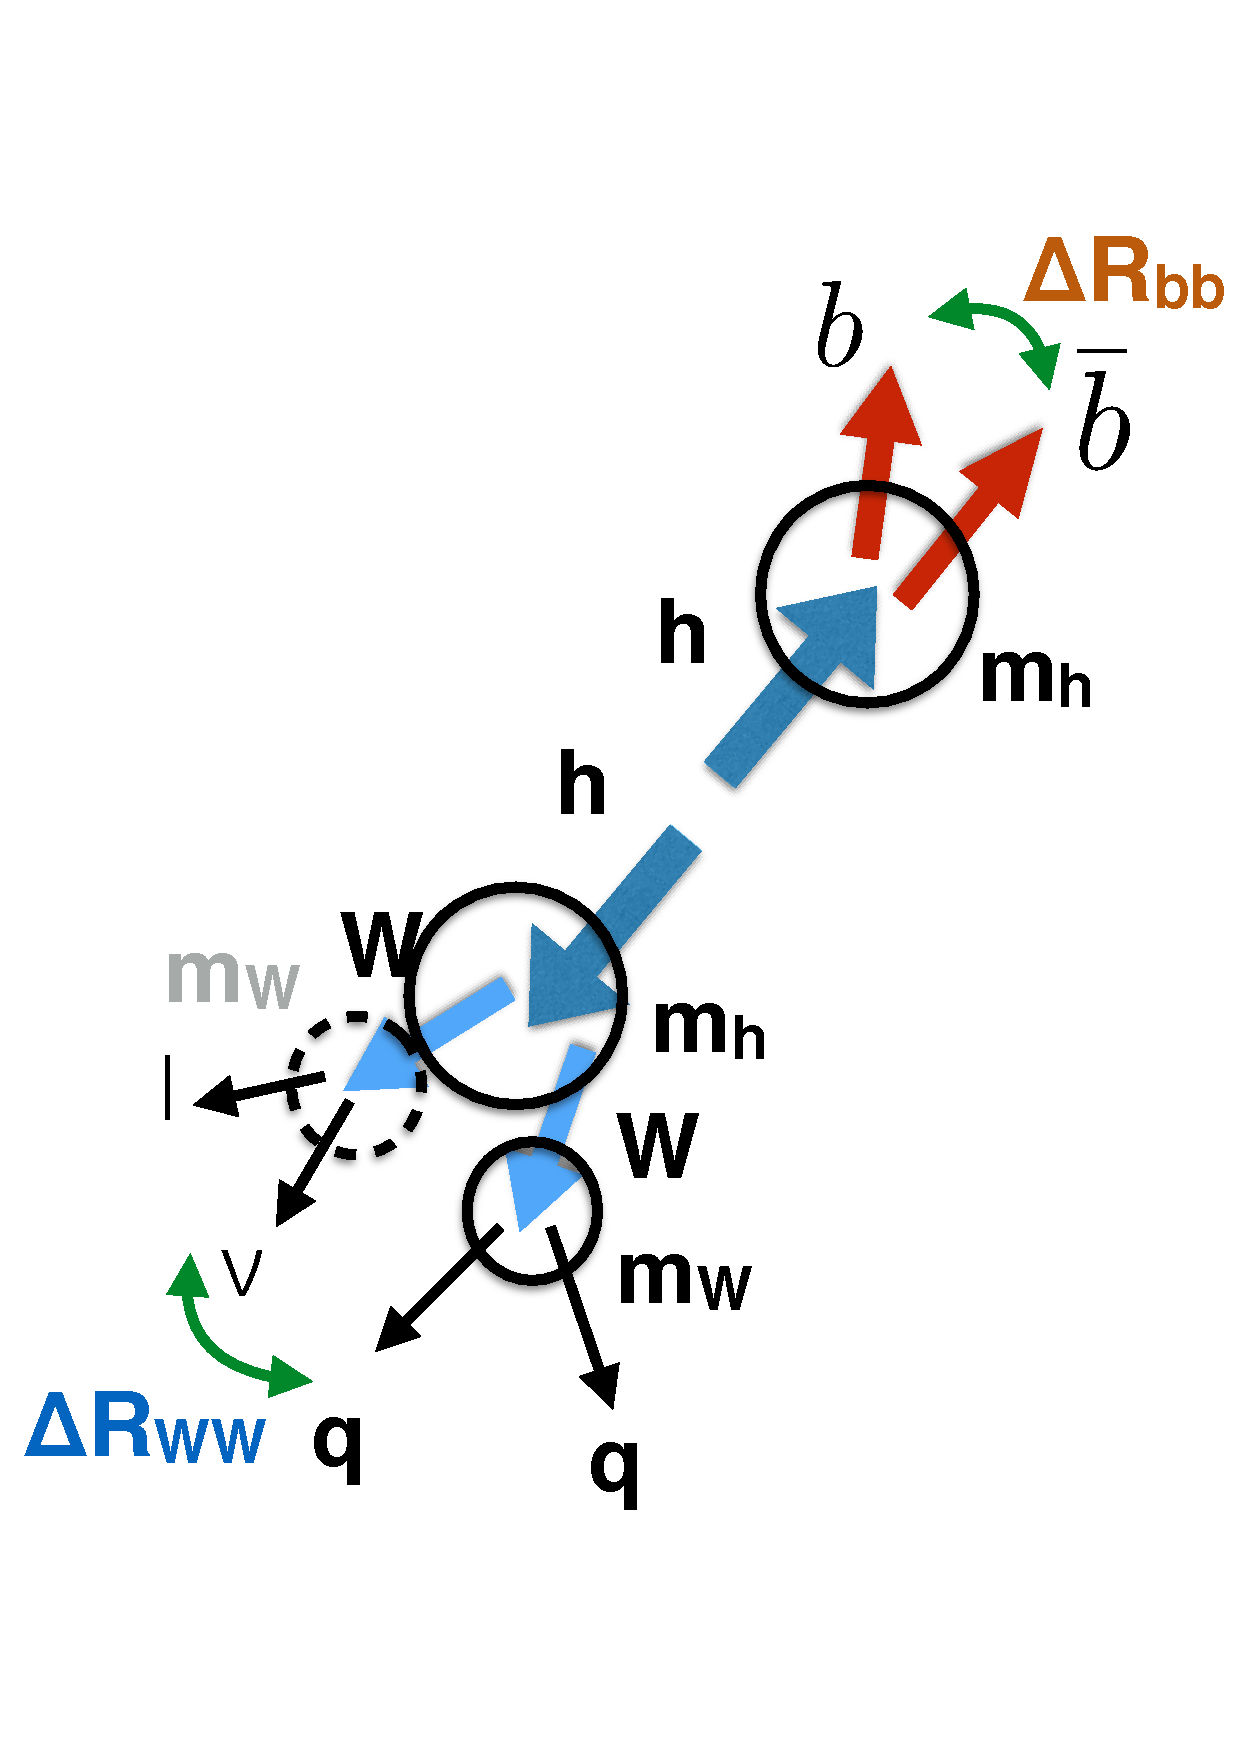
\includegraphics[width=0.4\textwidth]{figures/cartoon_hh.pdf}
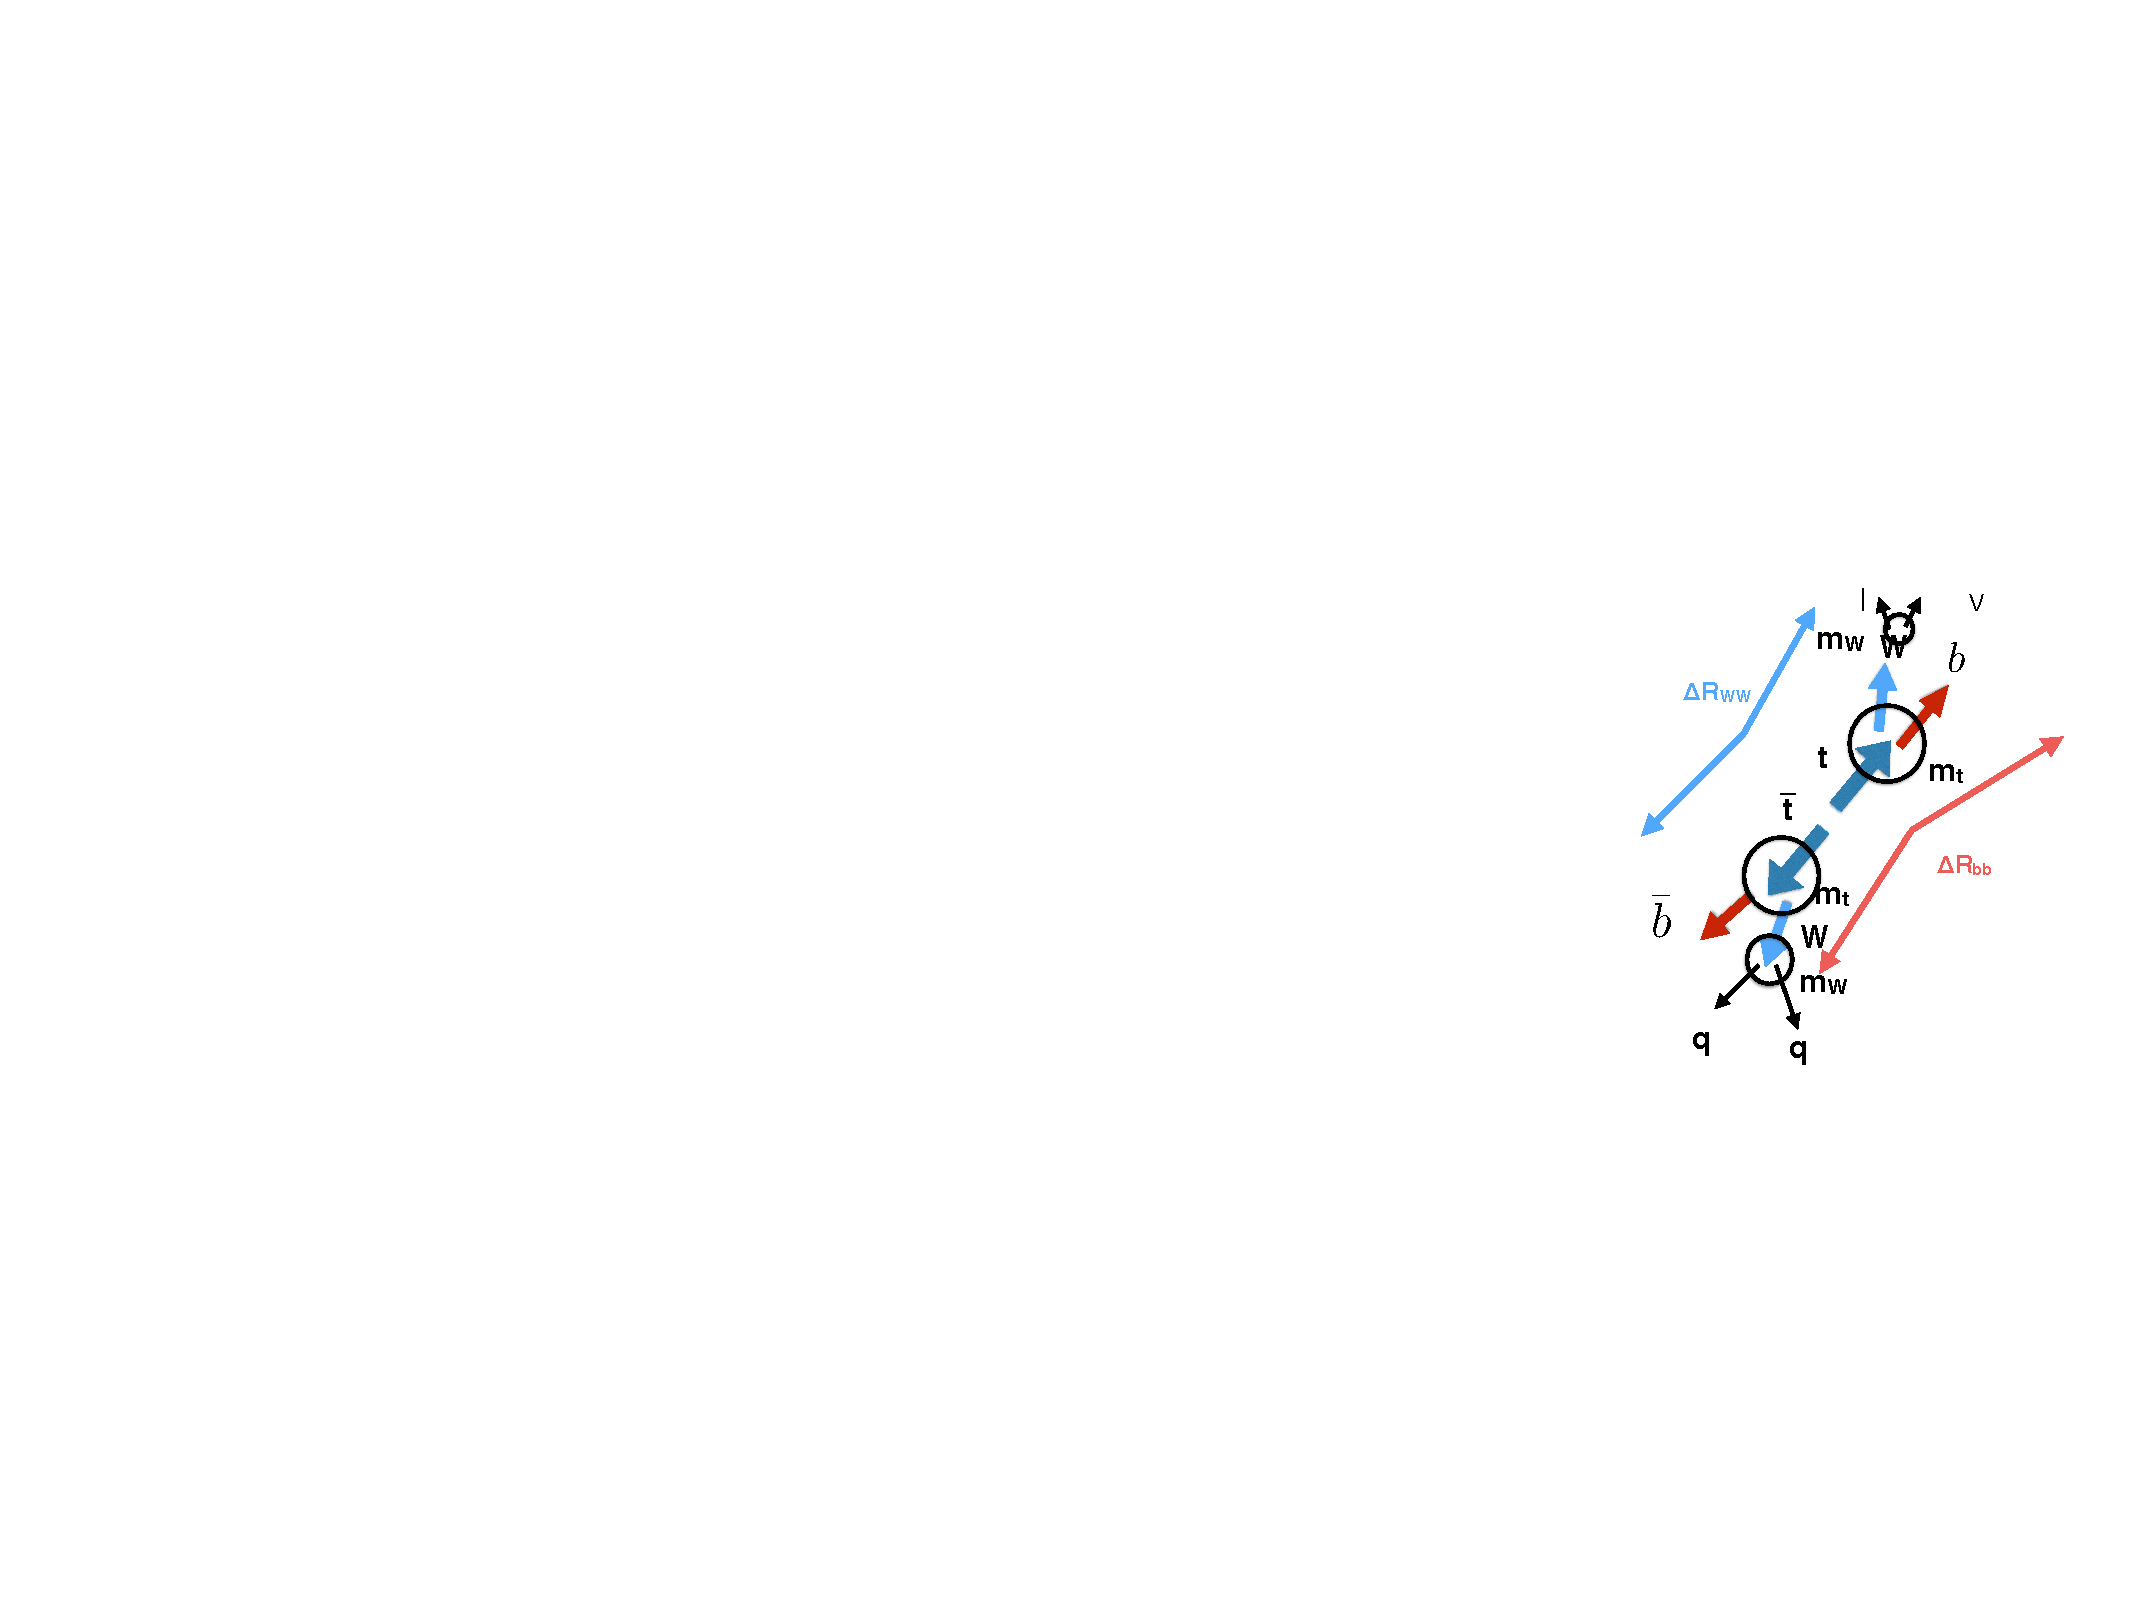
\includegraphics[width=0.4\textwidth]{figures/cartoon_tt.pdf}
\caption[Comparison signal and \ttbar events]{Schematic view of a $HH \to WWbb$ event compared to a $t\bar{t} \to WWbb$ event.} 
\label{fig:cartoon}
\end{figure}

The $t \bar{t}$ events are typically characterised by two $b$-jets and
two $W$ bosons such that the $\Delta R$ separation between the two
$b$-jets and between the $W$ bosons is large. On the contrary, in particular
when the invariant mass of the $m_{HH}$ is high, the signal is characterised
by two $b$-jets which are close together in $\Delta R$ and by two $W$ bosons
which are also relatively closer than in the $t \bar{t}$
case. Moreover, while for the signal the two $b$-jets have an
invariant mass equal to $m_h$, this is not necessarily the case for the $t \bar{t}$ background.  Following these considerations, the typical separation variables are: 
\begin{itemize}
\item the $p_T$ of the $b \bar{b}$ pair ($p_T^{bb}$);
\item the $\Delta R$ of the $b \bar{b}$ pair ($\Delta R^{bb}$);
\item the $p_T$ of the $WW$ pair ($p_T^{WW}$);
\item the $\Delta R$ of the $WW$ pair ($\Delta R^{WW}$);
\item the mass of the $WW$ system computed using the calculated neutrino
      longitudinal momentum ($m_{\rm WW}$). This value is exactly equal to $m_h$
      if a real solution is found, it is larger if no real solution is found;
\item the invariant mass of the di-Higgs boson candidate system ($m_{HH}$). 
\item the invariant mass of the 2 b-jets boson system ($m_{bb}$). 

\end{itemize}


\subsection{Signal region definitions}
\label{subsec:SR}
The cuts of the selection have been optimised by maximising the Poisson
significance at the end of the selection \footnote{a two step procedure has
been implemented. In the first step each cut is optimised, in the second step,
all cuts are set to their optimal value and cuts are varied one by one to
look for a different optimisation point. Correlation among variables 
could in fact spoil the results obtained at the first step.}. The Poisson
significance formula depends on the absolute yield of expected signal and
background events. For the optimisation formula the \ttbar background was
normalised to data with $m_{bb} < 100$ GeV or $m_{bb} > 140$ GeV, 
such region rejects, in fact, the majority of the signal. Four signal
hypotheses have been used in the optimisation:
\begin{itemize}
\item{ a heavy Higgs with $m_H = 500$ GeV and $m_H = 700$ GeV (defined as low-mass analysis)},
\item{ a heavy Higgs with $m_H = 2000$ GeV (defined as high-mass analysis) and}
\item{ a non-resonant di-Higgs production (defined as non-resonant analysis).}
\end{itemize}
An additional mass point with $m_H = 1400$ GeV was also checked. The resulting selection and the corresponding sensitivity are very similar to the selection for $m_H = 2000$ GeV, and hence that selection is dropped.{\footnote {See \url {https://indico.cern.ch/event/641988/contributions/2604588/attachments/1465307/2265002/bbWW_Weekly_Optimization_Revisited_24May2018.pdf}}} 
%The signals have been normalised to the Run 1 upper limit scaled by the $13/8$ TeV cross section ratio expected from the
%PDF luminosity scale of a narrow resonance of that mass. 

The signal regions for the  reference signal hypotheses are summarized in 
Table~\ref{tab:sig_reg_summary}.


\begin{table}
\begin{center}
\begin{tabular}{c|c|c|c|c}
 variable & \emph{Non-Res} & \emph{m500} & \emph{low-mass} & \emph{high-mass}\\
\hline
$E^{\rm T}_{miss}$ (GeV)		&$> 25$&$>25$&$> 25$& $> 25$ \\
$m_{WW}$ (GeV) 	   		&$< 130$ &$< 130$ & $< 130$& no-cut\\
$p_{\rm T}^{bb}$ (GeV) 		&$> 300$& $> 210$&$> 210$&$> 350$\\
$p_{\rm T}^{WW}$ (GeV) 		&$> 250$&$> 150$&$> 250$&$> 250$ \\
$\Delta R_{WW}$  		&no-cut& no-cut&no-cut&$<1.5$\\
$m_{bb}$ (GeV)   		&105-135&105-135&105-135&105-135\\
\end{tabular}
\caption[Criteria for non-resonant, \emph{m500}, \emph{low-mass} and 
    \emph{high-mass} selection]{Criteria for non-resonant, \emph{m500}, \emph{low-mass} and 
    \emph{high-mass} selection. The $m_{hh}$ window cut is not applied for 
    non-resonant signal, and for resonant signals $m_{hh}$ depends on 
    the mass.} 
\label{tab:sig_reg_summary}
\end{center}
\end{table}


The \textit{non-res} and \textit{m500} selections are exclusively used for non-resonant signal and resonant signal with mass 500 GeV respectively. The \textit{low-mass} selection is used for signal masses from 600 to 1300 GeV, while the \textit{high-mass} selection is used for signals with masses between 1400 and 3000 GeV. In addition, requirements are placed on the reconstructed di-Higgs invariant mass ${m_{HH}}$ as a function of the signal resonance mass ${m_{X}}$, as shown in Table \ref{tab:mhh_sig_cuts}. The resolution of the reconstructed mH H ranges from 6\% at 500 GeV to 10\% at 3000 GeV.

\begin{table}
\begin{center}
\begin{tabular}{c|c|c|c|c|c}
$m_{H}$ (GeV)      &   500   &   600   &   700   &   750   &   800 \\
$m_{hh}$ cut (GeV) & 480-530 & 560-640 & 625-775 & 660-840 & 695 - 905 \\ 
\hline 
$m_{H}$ (GeV)      &  900   &   1000  	   &  1100   	&  1200   		&   1300    \\
$m_{hh}$ cut (GeV) & 760-970	& 840-1160 & 925-1275	&1010-1390	&1095-1505  \\
\hline 
$m_{H}$ (GeV)      &   1400  		&  1500   		&  1600   		& 1800  		& 2000\\
$m_{hh}$ cut (GeV) &1250-1550	&1340-1660	&1430-1770	& 1750-2020 	& 1910-2170\\
\hline

\hline 
$m_{H}$ (GeV)      &   2250  		&  2500   		&  2750   		& 3000  		& \\
$m_{hh}$ cut (GeV) &2040-2460	&2330-2740	&2570-2950	& 2760-3210 	& \\
\end{tabular}
\caption[Window cuts on ${m_HH}$]{Window cuts on $m_{H}$ as a function of the resonance mass
  $m_{S}$.}
\label{tab:mhh_sig_cuts}
\end{center}
\end{table}


\subsection{Background Determination}
In the present analysis we expect that at the end of the event selection the
sample will be largely dominated by $t \bar{t}$ and multi-jet background, therefore the $t\bar{t}$ background normalisation
is derived from data while, as described in Sec. \ref{sec:multijet}, the multi-jet
background is derived using a data-driven ABCD method.
For all the other backgrounds, e.g. di-boson, Higgs, $W$+jets, the
MC is used appropriately normalized by using the expected cross sections and the
integrated luminosity that has been collected.

\subsubsection{Top normalization and control region}
\label{subsec:topCR}
The \ttbar background is normalised and validated using  dedicated
control regions (CR). Three CR's are defined, one for the SR's of the non-resonant (CR1), one for the low-mass analysis (CR2), and one for the high-mass analysis (CR3).  The CRs are defined in Table \ref{tab:CRdef}.


Table \ref{tab:CR1} through \ref{tab:CR3} show the number of observed
events and expected background events in the top CRs, and also in the sideband across selections that serve as validation regions. The final signal region is defined by $m_{bb}$ cut of $105~\textrm{GeV} < m_{bb} < 135~\textrm{GeV}$ based on optimization. The sidebands are orthogonal to the SR by virtue of having the $m_{bb}$ cut reversed. $m_{bb} < 100$ GeV or $m_{bb} > 140$ GeV defines the sidebands in which the control regions are defined.  The 5 GeV buffer region is kept on both sides so as to be less affected by systematic effects at the edge. Fig.~\ref{fig:mbb_signal} shows $m_{bb}$ for various signal mass points. A comparative study of signal over background in these three regions shows that S/B in the final SR is 5 (20) times higher than in the sidebands for m2000 (non-resonance) while S/B in the final SR is approximate twice as high as in the buffer zones.  Table~\ref{tab:sigOverBkg} shows the ratios of S/B in the buffer zones and sidebands compared to the S/B in the final SR. 

\begin{figure}[!h]
\begin{center}
\includegraphics*[width=0.47\textwidth] {figures/bbMass_X500_X700_X1400_X2000_X3000.eps}
\caption[$m_{bb}$ resolution for signal and sum of backgrounds.]{$m_{bb}$ resolution for signal samples.}
\label{fig:mbb_signal}
\end{center}
\end{figure}

\begin{table}
\begin{center}
\begin{tabular}{c|c|c|c|c|}
Selection & non-res & m500 & m700 & m2000\\
\hline
Buffer/SR              	& 1.85 & 1.95  & 1.90 & 1.63\\
\hline
 Sidebands/SR	       & 20.5 & 12.6 & 13.4 & 5.6\\
\hline 
\end{tabular}
\caption[S/B ratios]{The ratios of S/B in the buffer zone and sidebands compared to the S/B in the final SR. } 
\label{tab:sigOverBkg}
\end{center}
\end{table}

\newpage
%%%%%%%%%%%%%%
\begin{table}
\begin{center}
%\begin{tabular}{c|c|c|c|c|cxs}
% variable 						& Non-Res 	 	& X700 		& X2000\\
%\hline
%$m_{WW}$ (GeV)   				& $<130$ 		   	&$<130$ 		& no-cut \\
%$p_{\rm T}^{bb}$ (GeV) 			& $>150$ 		  	& $>150$ 		&$>350$\\
%$\Delta R_{bb}$  				& no-cut 	 		& no-cut		& no-cut  \\
%$p_{\rm T}^{WW}$ (GeV) 			& no-cut	 	 	& no-cut   		& no-cut \\
%$\Delta R_{WW}$  				& no-cut 		 	& no-cut 		& no-cut \\
%$m_{hh}$ (GeV)  				& no-cut 			& no-cut 		& no-cut\\
%\hline
\begin{tabular}{c|c|c|c|}
 variable 						&CR1 				& CR2 	& CR3 \\
\hline					
$m_{bb}$ (GeV)						& $m_{bb} < 100$ or $m_{bb} > 140$ & $m_{bb} < 100$ or $m_{bb} > 140$ & $m_{bb} < 100$ or $m_{bb} > 140$\\
$m_{WW}$ (GeV)   				& $<130$ 		 		& $<130$		& no-cut \\
$p_{\rm T}^{bb}$ (GeV) 			& $>300$ 		 		& $>210$		&$>350$\\
\hline


\end{tabular}
\caption[Definition of the kinematic regions used to normalise the Top background]{Definition of the kinematic regions used to normalise the Top background. $m_{bb} < 100$~GeV or $m_{bb} > 140~GeV$ defines the sidebands in which the control regions are defined. Expected SM backgrounds are then checked against data at each subsequent selection.} \label{tab:CRdef}
\end{center}
\end{table}
%%%%%%%%%%%%%%%
\iffalse
\begin{table}
\begin{center}
\begin{tabular}{c|c}
\hline
\multicolumn{2}{c}{Top CR definitions} \\
\hline
non-res  &  ($m_{bb} < 100$ GeV or $m_{bb} > 140$ GeV ), $m_{WW} < 130$ GeV  and $p_T^{\rm bb} > 150$ GeV (to be edited) \\
low-mass &  ($m_{bb} < 100$ GeV or $m_{bb} > 140$ GeV ), $m_{WW} < 130$ GeV  and $p_T^{\rm bb} > 150$ GeV \\
high-mass &   ({$m_{bb} < 100$ GeV or $m_{bb} > 140$ GeV}) and $p_T^{\rm bb} > 350$ GeV \\
\hline
\end{tabular}
\caption{Definition of the kinematic regions used to normalise the Top background.} \label{tab:CRdef}

\end{center}
\end{table}
\fi
%%tables to be added yet


\newpage

\begin{center}
\begin{table}
\begin{tabular}{l|c|c|c|c}
\hline\hline
\multicolumn{5}{c}{\textbf{CR1}: \mbb Sideband}\\\hline\hline
Sample  	& mww 	& bbpt210 	& bbpt300 	& wwpt250 	  \\\hline
\ttbar 	& 23776.6 $\pm$ 87.2 	& 531.7 $\pm$ 13.1 	& 109.9 $\pm$ 5.9 	& 63.9 $\pm$ 4.6 \\\hline 
QCD 	& 13310.5 $\pm$ 500.3 	& 250.2 $\pm$ 30.6 	& 33.7 $\pm$ 4.1 	& 21.4 $\pm$ 2.6	\\\hline 
W+jets 	& 3938.9 $\pm$ 31.1 	& 124.7 $\pm$ 3.5 	& 29.3 $\pm$ 1.4 	& 17.1 $\pm$ 1.1 	\\\hline 
SingleTop 	& 1605.4 $\pm$ 18.0 	& 76.0 $\pm$ 3.8 	& 20.1 $\pm$ 2.0 	& 13.5 $\pm$ 1.7\\\hline 
Dibosons 	& 109.9 $\pm$ 2.7 	& 8.3 $\pm$ 0.8 	& 2.2 $\pm$ 0.4 	& 1.5 $\pm$ 0.4 	\\\hline 
Z+jets 	& 1107.6 $\pm$ 8.4 	& 27.1 $\pm$ 0.8 	& 6.7 $\pm$ 0.4 	& 2.4 $\pm$ 0.2 	\\\hline 
\hline
Background Sum 	& 43849.0$\pm$ 509.2 	& 1017.9$\pm$ 33.7 	& 201.9$\pm$ 7.6 	& 119.8$\pm$ 5.7 \\\hline 
\hline
XhhSM 	& 44.6 $\pm$ 2.2 	& 9.1 $\pm$ 0.7 	& 1.5 $\pm$ 0.2 	& 1.1 $\pm$ 0.1 	\\\hline 
Data 	& 43902.0 	& 1069.0 	& 206.0 	& 138.0 \\\hline 
\hline
\end{tabular}
\caption[The number of events in the $m_{bb}$ sideband for the non-res selection]{ The number of observed
events and expected background events in the $m_{bb}$ side-bands for
the non-resonant selection. The top CR1 is defined at the bbpt300
selection. No NF has been applied to the background yields to show the level of data/expectation agreement before normalizing ttbar.  Only statistical uncertainties are shown.}
\label{tab:CR1}
\end{table}
\end{center}

\begin{center}
\begin{table}
\begin{tabular}{l|c|c|c|c}
\hline\hline
\multicolumn{5}{c}{\textbf{CR2}: \mbb Sideband}\\\hline\hline
Sample  	& mww 	& bbpt210 	& wwpt150 	& hh500  \\\hline
\ttbar 	& 23776.6 $\pm$ 87.2 	& 531.7 $\pm$ 13.1 	& 432.7 $\pm$ 11.8 	& 35.5 $\pm$ 3.2 		\\\hline 
QCD 	& 13310.5 $\pm$ 500.3 	& 250.2 $\pm$ 30.6 	& 206.3 $\pm$ 25.3 	& 16.9 $\pm$ 2.1 		\\\hline 
W+jets 	& 3938.9 $\pm$ 31.1 	& 124.7 $\pm$ 3.5 	& 105.9 $\pm$ 3.3 	& 4.9 $\pm$ 0.6 	\\\hline 
SingleTop 	& 1605.4 $\pm$ 18.0 	& 76.0 $\pm$ 3.8 	& 64.9 $\pm$ 3.5 	& 2.8 $\pm$ 0.6 	\\\hline 
Dibosons 	& 109.9 $\pm$ 2.7 	& 8.3 $\pm$ 0.8 	& 6.7 $\pm$ 0.8 	& 0.9 $\pm$ 0.2 	\\\hline 
Z+jets 	& 1107.6 $\pm$ 8.4 	& 27.1 $\pm$ 0.8 	& 19.0 $\pm$ 0.7 	& 1.5 $\pm$ 0.2 		\\\hline 
\hline
Background Sum 	& 43849.0$\pm$ 509.2 	& 1017.9$\pm$ 33.7 	& 835.5$\pm$ 28.3 	& 62.5$\pm$ 3.9	\\\hline 
\hline
Xhh500 	& 3.2 $\pm$ 0.1 	& 0.6 $\pm$ 0.1 	& 0.6 $\pm$ 0.1 	& 0.2 $\pm$ 0.1 	\\\hline 
Data 	& 43902.0 	& 1069.0 	& 898.0 	& 73.0 	\\\hline 
\end{tabular}
\caption[Events in $m_{bb}$ side band for the m500 selection]{ The number of observed
events and expected background events in the $m_{bb}$ side-bands for the low-mass selection, m500. The top CR2 is defined at the bbpt210 selection. To show how well the prediction matches data, no NF has been applied to any background. Only statistical uncertainties are shown.}
\label{tab:CR2_500}
\end{table}
\end{center}
%%%%%%%%%%%%%%%%%
\begin{center}
\begin{table}
\begin{tabular}{l|c|c|c|c}
\hline\hline
\multicolumn{5}{c}{\textbf{CR2}: \mbb Sideband}\\\hline\hline
Sample  	& mww 	& bbpt210 	& wwpt250 	& hh700   \\\hline
\ttbar 	& 23776.6 $\pm$ 87.2 	& 531.7 $\pm$ 13.1 	& 175.6 $\pm$ 7.5 	& 49.9 $\pm$ 3.9 	\\\hline 
QCD 	& 13310.5 $\pm$ 500.3 	& 250.2 $\pm$ 30.6 	& 72.4 $\pm$ 8.9 	& 28.4 $\pm$ 3.5 		\\\hline 
W+jets 	& 3938.9 $\pm$ 31.1 	& 124.7 $\pm$ 3.5 	& 45.7 $\pm$ 2.1 	& 13.7 $\pm$ 1.4 	\\\hline 
SingleTop 	& 1605.4 $\pm$ 18.0 	& 76.0 $\pm$ 3.8 	& 28.4 $\pm$ 2.4 	& 6.9 $\pm$ 1.1 		\\\hline 
Diboson 	& 109.9 $\pm$ 2.7 	& 8.3 $\pm$ 0.8 	& 2.8 $\pm$ 0.5 	& 0.7 $\pm$ 0.2 		\\\hline 
Z+jets 	& 1107.6 $\pm$ 8.4 	& 27.1 $\pm$ 0.8 	& 5.8 $\pm$ 0.4 	& 2.0 $\pm$ 0.3 		\\\hline 
\hline
Background Sum 	& 43849.0$\pm$ 509.2 	& 1017.9$\pm$ 33.7 	& 330.7$\pm$ 12.1 	& 101.5$\pm$ 5.5 	\\\hline 
\hline
Xhh700 	& 4.2 $\pm$ 0.2 	& 2.2 $\pm$ 0.1 	& 1.5 $\pm$ 0.1 	& 1.0 $\pm$ 0.1 	\\\hline 
Data 	& 43902.0 	& 1069.0 	& 367.0 	& 124.0	\\\hline 


\end{tabular}
\caption[Events in $m_{bb}$ side band for the m700 selection]{ The number of observed
events and expected background events in the $m_{bb}$ side-bands for the low-mass selection, m700. The top CR2 is defined at the bbpt210 selection. To show how well the prediction matches data, no NF has been applied to any background. Only statistical uncertainties are shown.}
\label{tab:CR2_700}
\end{table}
\end{center}
%%%%%%%%%%%%%%%%%%%
\begin{center}
\begin{table}
\begin{center}
\begin{tabular}{l|c|c|c|c}
\hline\hline
\multicolumn{5}{c}{\textbf{CR3}: \mbb Sideband}\\\hline\hline
Sample  	& bbpt350 	& wwpt250 	& drww15 	& hh2000 	\\\hline
\ttbar 	& 8568.7 $\pm$ 52.1 	& 7095.6 $\pm$ 47.5 	& 1940.5 $\pm$ 25.1 	& 122.3 $\pm$ 6.5 \\\hline 
QCD 	& 1538.7 $\pm$ 252.7 	& 1359.5 $\pm$ 75.9 	& 392.7 $\pm$ 21.9 	& 20.7 $\pm$ 1.2 	\\\hline 
W+jets 	& 2259.5 $\pm$ 7.9 	& 1952.1 $\pm$ 7.4 	& 696.6 $\pm$ 4.6 	& 55.5 $\pm$ 1.1 	\\\hline 
SingleTop 	& 1778.1 $\pm$ 19.4 	& 1601.6 $\pm$ 18.4 	& 405.4 $\pm$ 9.2 	& 29.6 $\pm$ 2.6 	\\\hline 
Dibosons 	& 170.6 $\pm$ 3.9 	& 147.1 $\pm$ 3.7 	& 46.8 $\pm$ 2.1 	& 3.4 $\pm$ 0.6 	\\\hline 
Z+jets 	& 403.6 $\pm$ 2.1 	& 307.6 $\pm$ 1.8 	& 95.6 $\pm$ 1.1 	& 7.5 $\pm$ 0.3 	\\\hline 
\hline
Background Sum 	& 14719.1$\pm$ 258.9 	& 12463.5$\pm$ 91.8 	& 3577.5$\pm$ 35.0 	& 238.9$\pm$ 7.2	\\\hline 
\hline
Xhh2000 	& 25.7 $\pm$ 0.4 	& 24.0 $\pm$ 0.4 	& 9.6 $\pm$ 0.3 	& 2.9 $\pm$ 0.1	\\\hline 
Data 	& 14862.0 	& 12450.0 	& 3761.0 	& 250.0 	\\\hline 

\end{tabular}
\end{center}
\caption[Events in $m_{bb}$ side band for the high-mass selection]{ The number of observed
events and expected background events in the $m_{bb}$ side-bands for
the high-mass selection. The top CR3 is defined at the bbpt350
selection. No NF has been applied to the background yields. Only statistical uncertainties are shown.}
\label{tab:CR3}
\end{table}
\end{center}

\begin{table}
\begin{center}
\begin{tabular}{c|c|c|c}
\multicolumn{4}{c}{Top background normalisation factors in the two
  CRs.} \\
\hline
region & NF & $\sigma_{stat.}$ & $\sigma_{syst.}$ \\
\hline
non-res   & 1.04  &  $\pm$0.20  &  $\pm$0.43\\
low-mass  & 1.14  &  $\pm$0.10  &  $\pm$0.35\\
high-mass & 1.02  &  $\pm$0.02  &  $\pm$0.07\\
\hline
\end{tabular}
\caption[Normalization factors for the two CRs]{Normalization factors for the two CRs, the statistical error
  includes only data statistics, the systematic error is obtained
  subtracting in quadrature the statistical error from the total error.} \label{tab:NFs}
\end{center}
\end{table}

Table \ref{tab:CR1} through \ref{tab:CR3} show the number of observed
events and expected background events in the top CRs before the
normalisation factors have been applied to the top background sample.

The top normalisation factors are determined by a simultaneous fit  of
signal and control regions, which include both Top CR and QCD CR~\ref{sec:multijet}. It also depends slightly on the $m_{hh}$ window due to the presence of top background in the signal region, and it is furthermore different for the \emph{non  res}, \emph{low  mass} and \emph{high mass} analyses. The normalisation
factors of the three top control regions are shown in Table \ref{tab:NFs}.

Fig.~\ref{fig:mbb_mhh} shows the $m_{bb}$ and $m_{hh}$ distributions in the two CRs.% while in Appendix \ref{app:data_exp_reOptNonRes} through ~\ref{app:data_exp_reOpt2000} we show the complete distributions of the
relevant variables used in the analysis selection in the top CR.  

\begin{figure}[!h]
\begin{center}
\includegraphics*[width=0.47\textwidth] {figures/ControlPlots_new/reOptNonRes/C_reOptNonRes_mww_bbpt210_bbpt300_bbMass_regionA_met25d020}
\includegraphics*[width=0.47\textwidth] {figures/ControlPlots_new/reOptNonRes/C_mBBcr_reOptNonRes_mww_bbpt210_bbpt300_hhMass_regionA_met25d020}

\includegraphics*[width=0.47\textwidth] {figures/ControlPlots_new/reOpt700/C_reOpt700_mww_bbpt210_bbMass_regionA_met25d020}
\includegraphics*[width=0.47\textwidth] {figures/ControlPlots_new/reOpt700/C_mBBcr_reOpt700_mww_bbpt210_hhMass_regionA_met25d020}

\includegraphics*[width=0.47\textwidth] {figures/ControlPlots_new/reOpt2000/C_reOpt2000_bbpt350_bbMass_regionA_met25d020}
\includegraphics*[width=0.47\textwidth] {figures/ControlPlots_new/reOpt2000/C_mBBcr_reOpt2000_bbpt350_hhMass_regionA_met25d020}

\caption[$m_{bb}$ and $m_{hh}$ in CR1, CR2 and CR3.]{$m_{bb}$ and $m_{hh}$ in CR1, CR2 and CR3.  \ttbar NFs as described in~\ref{subsec:topCR} have been applied. The uncertainties shown include the statistical and systematic uncertainties described in ~\ref{sec:systematics}. Data are blinded in the region $100 < m_{bb} < 140 $. }
\label{fig:mbb_mhh}
\end{center}
\end{figure}

\pagebreak
\subsection{Multi-jet background}

\label{sec:multijet}
Multi-jet backgrounds can enter in the event selection if a jet from
heavy flavour decays is mis-identified as an electron or a muon and used
as a lepton in the analysis. Such phenomena are not accurately reproduced by MC
simulation, due to large uncertainties in the jet shower shape simulation
and uncertainties in muon fragmentation functions and kinematics. In order 
to estimate the contributions of multi-jet processes, a data-driven ABCD 
method is used to estimate this background in the present analysis.
%%Such methods are used extensively in the top group analyses.

The ABCD method uses three control regions (the B, C, and D regions) to estimate
the contribution of a given background in the signal (A) region. Cuts on two ideally
orthogonal variables are used to create the signal and various control regions, e.g. 
the A region passes both cuts, the B and C regions each pass one cut and fail the other, 
while the D region fails both cuts. The absolute value of the significance of the lepton 
impact parameter and the missing transverse energy (MET) are used as the two variables 
used to define the regions in the ABCD method for this analysis. The regions are thus 
defined 
\begin{itemize}
\item A region: MET $>$ 25 GeV, \dsig $<$ 2.0
\item B region: MET $<$ 25 GeV, \dsig $<$ 2.0
\item C region: MET $>$ 25 GeV, \dsig $>$ 2.0
\item D region: MET $<$ 25 GeV, \dsig $>$ 2.0
\end{itemize}
Figure~\ref{fig:abcdCartoon} shows a pictoral representation of the four regions.
\begin{figure}[h!]
\begin{center}
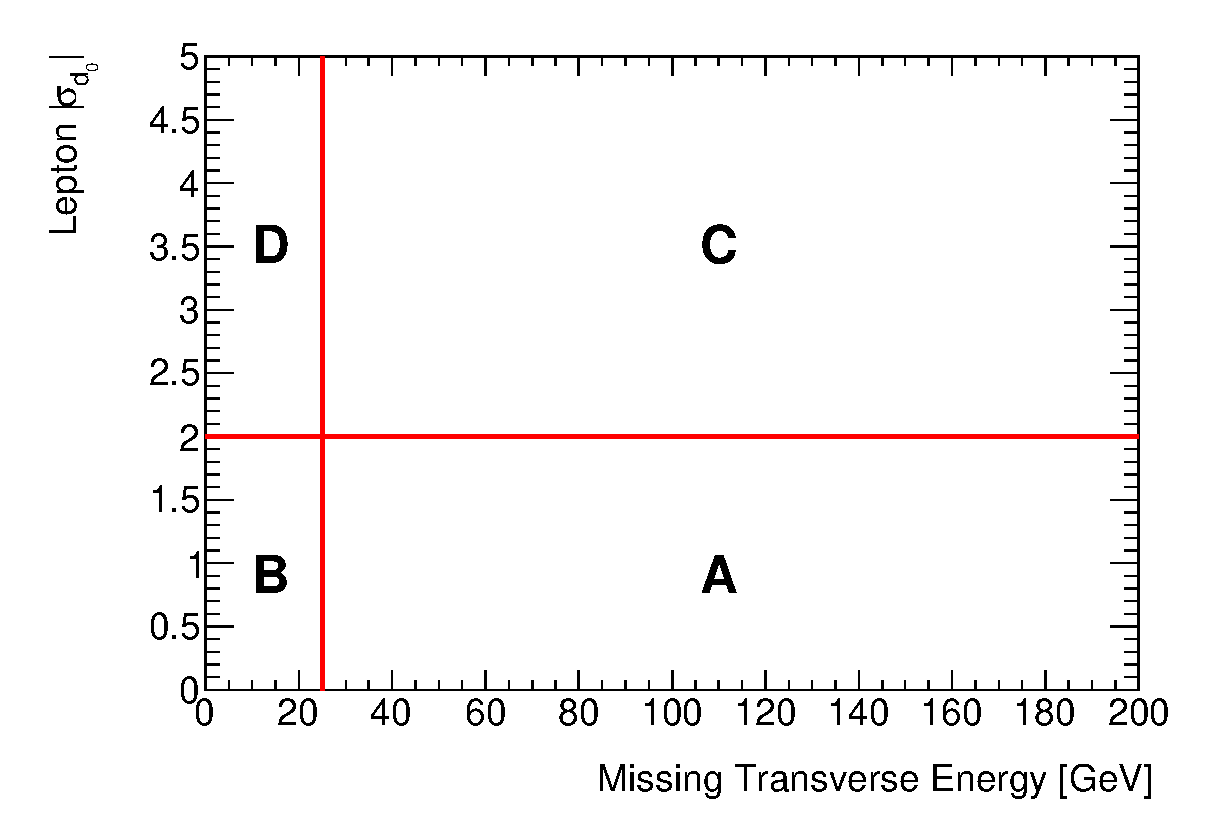
\includegraphics[width=0.6\textwidth]{figures/multijet/abcdExample_met_vs_d0sigBL20}
\end{center}
\caption{A pictoral representation of the four regions used in the
  ABCD calculation.} \label{fig:abcdCartoon}
\end{figure}
Assuming that the two variables chosen to define the ABCD regions are completely uncorrelated, the 
yield of the process being modelled (QCD multi-jets in this case) in the A region is given by
\begin{equation}
N_{A} = N_C \frac{N_B}{N_D}
\label{eq:simpleABCD}
\end{equation}
where the yields $N_i$ are yields calculated from data - all Monte Carlo backgrounds (\ttbar, 
W/Z+jets, single top, diboson processes) in region $i$ ($N_i = N_i^{\text{data}} - N_i^{\text{MC Bkgs}}$). 
The assumption underlying Equation~\ref{eq:simpleABCD} is that the relationship between the 
yields in the B and D regions is the same as the relationship between the A and C regions, i.e.
\begin{equation}
\frac{N_{A}}{N_{C}} = \frac{N_B}{N_D}
\label{eq:correlationStatement}
\end{equation}
Using equation ~\ref{eq:correlationStatement}, the quantity $R= \frac{N_{C} N_B}{N_{A} N_D}$ can be 
defined. In the case of two completely uncorrelated variables, $R=1$ and the ABCD estimation reduces 
to Equation~\ref{eq:simpleABCD}. If the two variables are not completely uncorrelated, the $R$ 
factor enters as a correction to Equation~\ref{eq:simpleABCD} for the multi-jet estimation in the A 
region, and the expression can be rewritten as
\begin{equation}
N_{A} = R \frac{N_C N_B}{N_D}
\label{eq:advancedABCD}
\end{equation}
The $R$ factor is calculated for each selection (non-resonant, low mass, and high mass) individually,
and the results at each cut in each selection is provided in
Table~\ref{tab:rValues}.


\begin{table}[h!]
\centering
\begin{tabular}{c|c|c|c}
\hline\hline
\multicolumn{4}{c}{QCD $R$ Values, Non-resonant Selection}\\\hline\hline
mww 	& bbpt210 	& bbpt300 	& wwpt250	\\\hline 
0.74 $\pm$ 0.04 	& 0.79 $\pm$ 0.23 	& 1.07 $\pm$ 1.18 	& ---	\\\hline \hline
%\end{tabular}

\multicolumn{4}{c}{QCD $R$ Values, Low Mass Selection (m500)}\\\hline\hline
mww 	& bbpt210 	& wwpt150 	& hh500	\\\hline 
0.74 $\pm$ 0.04 	& 0.79 $\pm$ 0.23 	& --- 	& ---	\\\hline \hline

%\begin{tabular}{c|c|c|c}
\multicolumn{4}{c}{QCD $R$ Values, Low Mass Selection (m700)}\\\hline\hline
mww 	& bbpt210 	& wwpt250 	& hh700	\\\hline 
0.74 $\pm$ 0.04 	& 0.79 $\pm$ 0.23 	& 0.09 $\pm$ 0.14 	& ---	\\\hline \hline
%\end{tabular}

%\begin{tabular}{c|c|c|c}
\multicolumn{4}{c}{QCD $R$ Values, High Mass Selection}\\\hline\hline
bbpt350 	& wwpt250 	& drww15 	& hh2000	\\\hline 
0.48 $\pm$ 0.09 	& 0.43 $\pm$ 0.08 	& 0.50 $\pm$ 0.16 	& 4.28 $\pm$ 5.30	\\\hline 
\hline\hline
\end{tabular}


\caption[Values of R at each selection]{Values calculated for $R$ at each stage in the non-resonant,
  low mass, and high mass selections. The estimate of multi-jet
  contribution in the A region uses the $R$ value calculated after the
  first cut of each selection.} \label{tab:rValues}
\end{table}
In order to minimize the statistical error on $R$, the $R$ value calculated after 
the first cut of each selection (0.74 and 0.48) is used in Equation~\ref{eq:advancedABCD} to estimate the multi-jet
background after each subsequent cut. This can be done given the
compatibility of the $R$ value at the end of the cut flow with that at
the point where $R$ is evaluated. In order to check such compatibility
with higher statistics, the $R$ value has been calculated applying
each selection cut just after the cut where $R$ is evaluated, in order
to check that $R$ is not correlated with each of the selection cuts.
The result is shown in Table \ref{tab:R_after_X}.

\begin{table}[h!]
\centering

\begin{tabular}{c|c|c|c}
\hline\hline

%\multicolumn{2}{c}{QCD $R$ Values, Non-resonant Selection}\\\hline\hline
%mww 	                & mww + bbpt210 	\\\hline 
%0.74 $\pm$ 0.04 	& 0.79 $\pm$ 0.23 	\\\hline \hline
%\multicolumn{2}{c}{QCD $R$ Values, Low Mass Selection}\\\hline\hline
%mww 	                & mww + bbpt210 	\\\hline 
%0.74 $\pm$ 0.04 	& 0.79 $\pm$ 0.23 	  \\\hline \hline
%\multicolumn{2}{c}{QCD $R$ Values, High Mass Selection}\\\hline\hline
%bbpt350 	        & bbpt350 + wwpt250 	\\\hline 
%0.48 $\pm$ 0.09 	& 0.43 $\pm$ 0.08 	\\\hline 


\multicolumn{4}{c}{QCD $R$ Values, Non-resonant Selection}\\\hline\hline
mww 	                & mww + bbpt210 	& mww + bbpt300 	& mww + wwpt250 	\\\hline 
0.74 $\pm$ 0.04 	& 0.79 $\pm$ 0.23 	& 1.12 $\pm$ 1.22 	& 0.25 $\pm$ 0.20 	\\\hline \hline
\multicolumn{4}{c}{QCD $R$ Values, Low Mass (m500) Selection}\\\hline\hline
mww 	                & mww + bbpt210 	& mww + wwpt150 	& mww + hh500	  \\\hline 
0.74 $\pm$ 0.04 	& 0.79 $\pm$ 0.23 	& 0.50 $\pm$ 0.08 	& 0.52 $\pm$ 0.09  \\\hline \hline
\multicolumn{4}{c}{QCD $R$ Values, Low Mass (m700) Selection}\\\hline\hline
mww 	                & mww + bbpt210 	& mww + wwpt250 	& mww + hh700	  \\\hline 
0.74 $\pm$ 0.04 	& 0.79 $\pm$ 0.23 	& 0.25 $\pm$ 0.20 	& 0.63 $\pm$ 0.13  \\\hline \hline
\multicolumn{4}{c}{QCD $R$ Values, High Mass Selection}\\\hline\hline
bbpt350 	        & bbpt350 + wwpt250 	& bbpt350 + drww15 	& bbpt350 + hh2000	\\\hline 
0.47 $\pm$ 0.06 	& 0.44 $\pm$ 0.08 	& 0.52 $\pm$ 0.17	& 1.07 $\pm$ 0.67 	\\\hline 

\hline\hline
\end{tabular}

\caption[Cross check for coorelation with R]{Values of $R$ obtained applying a single selection cut after the cut stage where $R$ is nominally evaluated.} \label{tab:R_after_X}
\end{table}


Once the normalization of the multi-jet background in the A region is calculated using Equation~\ref{eq:advancedABCD}, the shape of the multi-jet template is taken from the data - Monte Carlo distribution in the C region since the two are kinematically identical except for the cut on \dsig.

The uncertainty due to the limited statistics in the B and D regions is the
main source of the multi-jet estimation method systematics. In order to minimise
such error,  the yields from the  B and D regions used in the ABCD
calculation are frozen at a level of the cutflow to minimise statistical fluctuations.
The B and D region yields are frozen after the \ptbb $>$ 210 GeV cut for the non-resonant and low mass selection, and after the $p_{T}(WW)>$ 250 GeV for the high mass selection. Appendix~\ref{app:qcd_BDregionStudy_appendix} details the study carried out to select the stage at which to freeze the B and D regions. 

To further reduce the error coming from the C region, the shape of the data - Monte Carlo, i.e. non-prompt, 
\mbb distribution was studied as a function of each individual cut for each selection. If the \mbb shape is 
unchanged by the additions of cuts later in a given selection, the C region shape can be taken from an 
earlier stage in the cutflow, reducing the shape uncertainty and overall statistical error on the QCD yield.
To determine the stability of the \mbb shape, the ratio of events in the \mbb signal region ([100, 140] GeV)
over the numbers of events in the full \mbb spectrum was computed for each individual cut using the C region 
of the ABCD method. This ratio was found to be stable across each selection, and the results of this 
calculation are provided in Table~\ref{tab:efficiencyFactor}. 

  \begin{table}[h!]%\fontsize{8}{9}\selectfont
    \centering
    \begin{tabular}{c|c|c|c}
      \hline\hline
      \multicolumn{4}{c}{reOptNonRes: \mbb SR/Total Ratios For Individual Cuts}\\\hline\hline 
      mww 	& bbpt210 	& bbpt300 	& wwpt250 	\\\hline 
      0.17 $\pm$ 0.02 	& 0.15 $\pm$ 0.03 	& 0.13 $\pm$ 0.05 	& 0.16 $\pm$ 0.05 	\\\hline 
    \end{tabular}
    \vspace{5pt}
    
    \begin{tabular}{c|c|c|c}
      \hline\hline
      \multicolumn{4}{c}{reOpt500: \mbb SR/CR Ratios For Individual Cuts}\\\hline\hline 
      mww 	& bbpt210 	& wwpt150 	& hh500 	\\\hline 
      0.17 $\pm$ 0.02 	& 0.15 $\pm$ 0.03 	& 0.18 $\pm$ 0.02 	& 0.22 $\pm$ 0.03 	\\\hline 
    \end{tabular}
    \vspace{5pt}

    \begin{tabular}{c|c|c|c}
      \hline\hline
      \multicolumn{4}{c}{reOpt700: \mbb SR/Total Ratios For Individual Cuts}\\\hline\hline 
      mww 	& bbpt210 	& wwpt250 	& hh700 	\\\hline 
      0.17 $\pm$ 0.02 	& 0.15 $\pm$ 0.03 	& 0.16 $\pm$ 0.05 	& 0.16 $\pm$ 0.02 	\\\hline 
    \end{tabular}
    \vspace{5pt}

    \begin{tabular}{c|c|c|c}
      \hline\hline
      \multicolumn{4}{c}{reOpt2000: \mbb SR/Total Ratios For Individual Cuts}\\\hline\hline 
      bbpt350 	& wwpt250 	& drww15 	& hh2000 	\\\hline 
      0.12 $\pm$ 0.08 	& 0.16 $\pm$ 0.05 	& 0.19 $\pm$ 0.02 	& 0.11 $\pm$ 0.14 	\\\hline 
      \hline 
    \end{tabular}
    \caption[Ratio of events in SR over SR+CR]{The ratio of events in the \mbb signal region ([100, 140] GeV) over the numbers of events in the full \mbb spectrum for each individual cut. Both event yields are calculated in the C region of the ABCD method. The ratios are found to be stable across each selection.}        \label{tab:efficiencyFactor}
  \end{table}

The normalized shapes of the full \mbb distributions after each 
cut are shown in Figure~\ref{fig:mbbShapes}. The earliest selection cut with a consistent shape was chosen as the
shape for each cutflow and this corresponds to the shape obtained
after the  \ptbb $>$ 210 GeV cut 
for the non-resonant the m500 and m700  selections,  and after the  \ptww $>$ 250 GeV for the m2000 selection.

\begin{figure}[h!]
\begin{center}
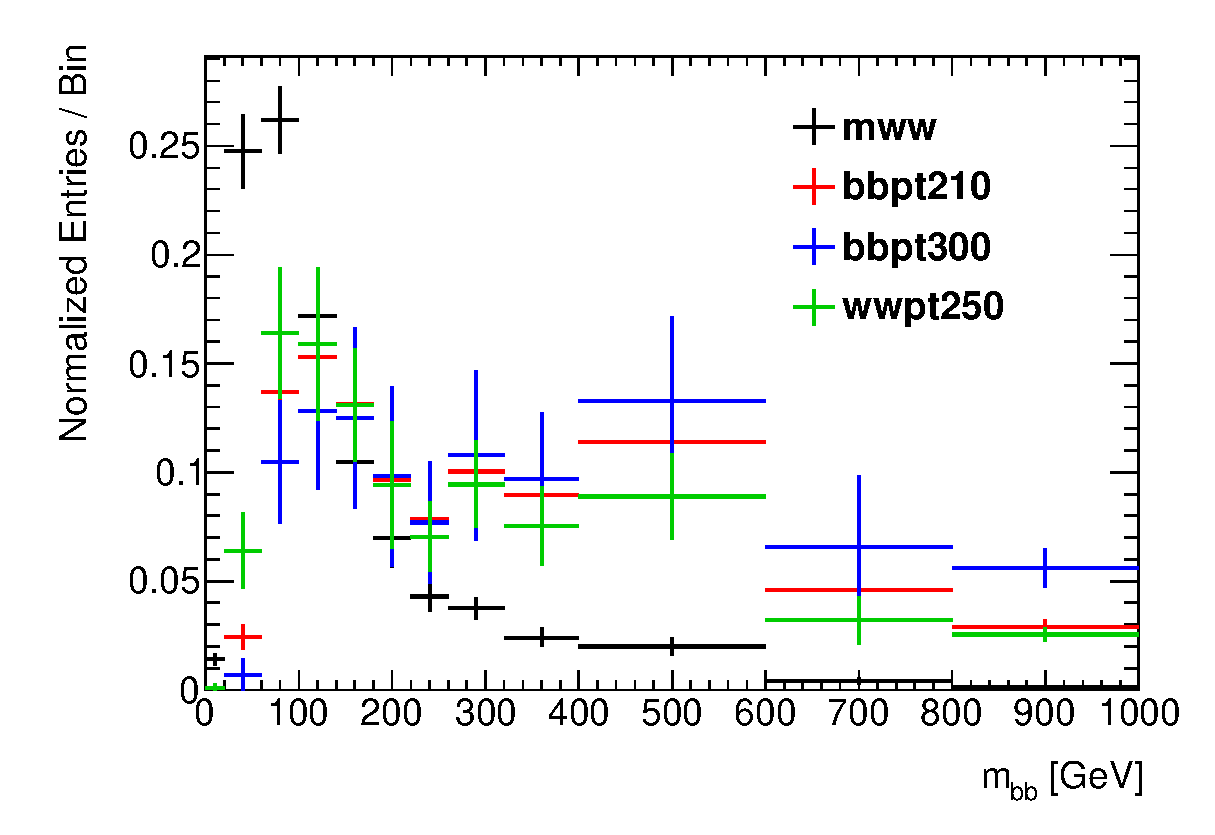
\includegraphics[width=0.4\textwidth]{figures/multijet/reOptNonRes_mbbShape_individualCuts_elmu}
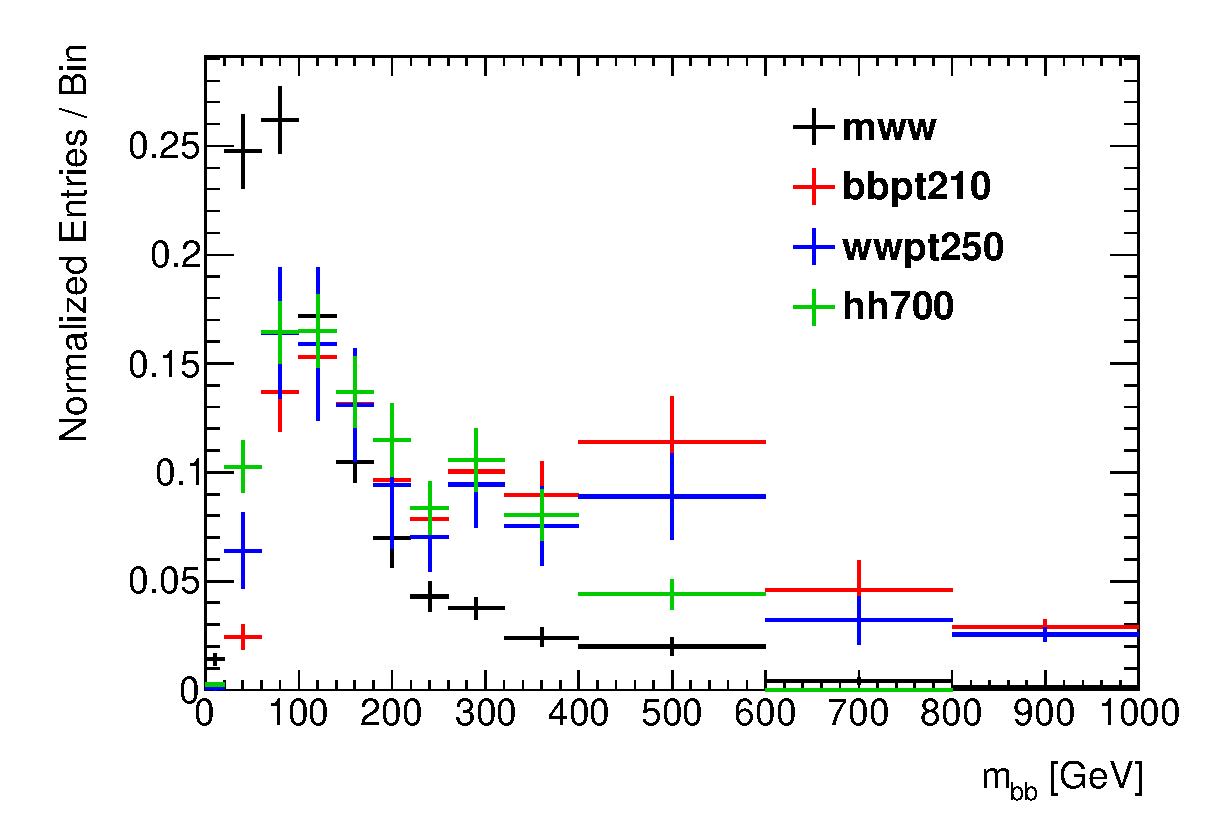
\includegraphics[width=0.4\textwidth]{figures/multijet/reOpt700_mbbShape_individualCuts_elmu}
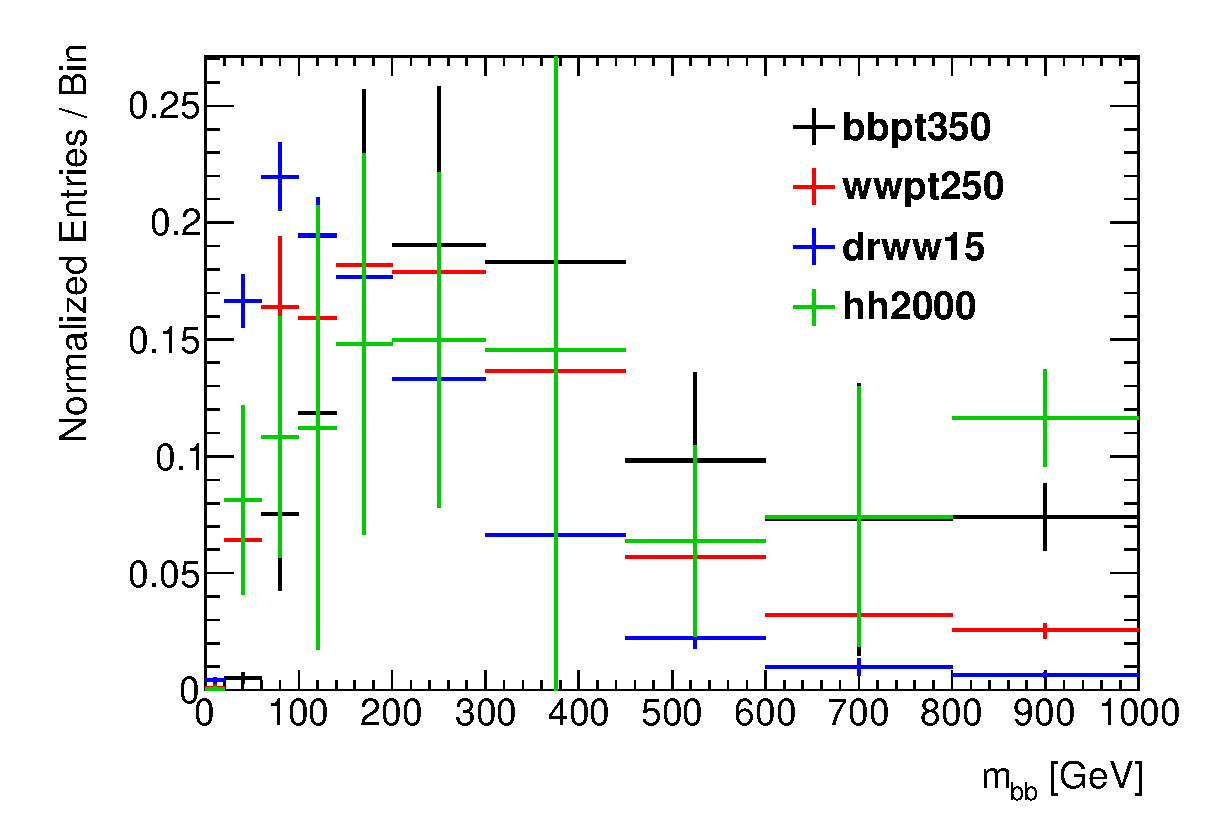
\includegraphics[width=0.4\textwidth]{figures/multijet/reOpt2000_mbbShape_individualCuts_elmu}
\end{center}

\caption[The normalized shapes of the full \mbb distributions]{The normalized shapes of the full \mbb distributions after
  each in each selection. Shapes from the non-resonant cutflow are
  shown at the top left, shapes from the low mass selection are shown
  at the top left, and shapes from the high mass selection are shown
  at the bottom. The earliest selection cut with a consistent shape
  was chosen as the shape for each cutflow and this corresponds to the
  shape obtained after the \mww and \ptbb $>$ 210 GeV cuts for the
  non-resonant and low mass selections and after the \ptbb $>$ 350 GeV
  and \ptww $>$ 250 GeV for the high mass mass selection.} \label{fig:mbbShapes}
\end{figure}

Since \ttbar and  multi-jet contaminate the control
regions used for their estimation,  additional studies were
performed via an iterative procedure to ensure that the \ttbar and QCD
yields converge to stable values and that the estimation technique is
able to disentangle between the two backgrounds.
Appendix~\ref{app:qcd_ttbarNFstability_appendix} details the results of the study, and the yields 
were found to converge (stable within $<5\%$) after a few iterations for each cutflow.

%Since the \mtw distribution should contain a large multi-jet contribution at low \mtw, the agreement 
%between data and prediction in the \mtw distribution for each selection acts as a closure test on 
%the estimation of the multi-jet background by the ABCD method. Appendices~\ref{app:data_exp_reOptNonRes}
%,~\ref{app:data_exp_reOpt700}, and~\ref{app:data_exp_reOpt2000} show these distributions in the 
%\ttbar control regions for each selection. Good agreement is observed.

To evaluate the systematic error of the estimation, a Sherpa multi-jet $bb$ sample is used to compare 
the ABCD prediction to the Monte Carlo expectation using events with exactly one lepton and four jets. 
No $b$-tagging requirements or other event selection cuts are applied. Pseudo-data is produced using
the multi-jet Monte Carlo and events from the nominal \ttbar Monte Carlo. The $R$ factor is calculated
using the inclusive $b$-tag (0, 1, or 2 $b$-tags) and used to estimate the QCD contribution in the two
$b$-tag exclusive region. The percent difference between the number of events from the ABCD estimation 
and the number of multi-jet events from Monte Carlo used to produce the pseudo-data is taken as the 
systematic uncertainty. This uncertainty is calculated to be 36\%. In addition, the $bb$ MC is used to
calculate the $R$ factor for each selection (non-resonant, low mass, and high mass) and each lepton 
channel, and the results at each cut in each selection are provided in the Table~\ref{tab:lepR}. 

\begin{table}[h!]
\centering
\begin{tabular}{c|c|c|c|c}

\hline\hline
\multicolumn{5}{c}{Non-resonant: QCD $R_{non-prompt}$ Values}\\\hline\hline 
          & mww                 & bbpt210 	        & bbpt300 	        & wwpt250	        \\ \hline 
Combined  & 0.74 $\pm$ 0.04 	& 0.80 $\pm$ 0.05  	& 0.64 $\pm$ 0.08 	& 0.62 $\pm$ 0.05	\\\hline 
Electrons & 0.72 $\pm$ 0.05  	& 0.75 $\pm$ 0.06 	& 0.68 $\pm$ 0.10 	& 0.64 $\pm$ 0.06	\\\hline 
Muons     & 0.81 $\pm$ 0.06 	& 0.92 $\pm$ 0.11 	& 0.55 $\pm$ 0.15 	& 0.59 $\pm$ 0.10	\\\hline 
\hline\hline
\multicolumn{5}{c}{Low-mass (m500): QCD $R_{non-prompt}$ Values}\\\hline\hline 
          & mww                 & bbpt210 	        & wwpt150 	        & hh500 	        \\ \hline 
Combined  & 0.74 $\pm$ 0.04 	& 0.80 $\pm$ 0.05 	& 0.68 $\pm$ 0.03  	& 0.50 $\pm$ 0.03	\\\hline 
Electrons & 0.72 $\pm$ 0.05 	& 0.75 $\pm$ 0.06 	& 0.65 $\pm$ 0.03 	& 0.44 $\pm$ 0.04	\\\hline 
Muons     & 0.81 $\pm$ 0.06 	& 0.92 $\pm$ 0.11 	& 0.75 $\pm$ 0.06 	& 0.58 $\pm$ 0.07	\\\hline 
\hline\hline

\multicolumn{5}{c}{Low-mass (m700): QCD $R_{non-prompt}$ Values}\\\hline\hline 
          & mww                 & bbpt210 	        & wwpt250 	        & hh700 	        \\ \hline 
Combined  & 0.74 $\pm$ 0.04 	& 0.80 $\pm$ 0.05 	& 0.62 $\pm$ 0.25 	& 0.60 $\pm$ 0.03	\\\hline 
Electrons & 0.72 $\pm$ 0.05 	& 0.75 $\pm$ 0.06 	& 0.64 $\pm$ 0.06 	& 0.52 $\pm$ 0.04	\\\hline 
Muons     & 0.81 $\pm$ 0.06 	& 0.92 $\pm$ 0.11 	& 0.59 $\pm$ 0.10 	& 0.74 $\pm$ 0.08	\\\hline 
\hline\hline


\multicolumn{5}{c}{High-mass: QCD $R_{non-prompt}$ Values}\\\hline\hline 
          & bbpt350             & wwpt250 	        & drww15 	        & hh2000 	        \\ \hline 
Combined  & 0.47 $\pm$ 0.09 	& 0.62 $\pm$ 0.05 	& 0.68 $\pm$ 0.03 	& 0.58 $\pm$ 0.13	\\\hline 
Electrons & 0.48 $\pm$ 0.10 	& 0.64 $\pm$ 0.06 	& 0.60 $\pm$ 0.04 	& 0.57 $\pm$ 0.14	\\\hline 
Muons     & 0.44 $\pm$ 0.20 	& 0.59 $\pm$ 0.10 	& 0.82 $\pm$ 0.07 	& 0.65 $\pm$ 0.39	\\\hline 
\hline\hline


\end{tabular}
\caption[$R_{non-prompt}$]{$R_{non-prompt}$ calculated for the QCD Monte Carlo sample at using each cut individually from all selections. The lepton channels are shown separated and combined.}
\label{tab:lepR}
\end{table}










\subsection{Background Shape and Cutflow}
\label{sec:systematics}
 The modelling of the background was checked at all selection
stages and, in general, shows good agreement with data.
Figure~\ref{fig:resolved_mtlep} shows the $\mT$ distribution of the
leptonic $W$ boson candidate  in the three
top control regions. The $\mT$ variable is defined as:
\[
\mT = \sqrt{2\pt^{\ell}\met\cdot (1-\rm{cos}\Delta \phi)} ~,
\]
where $\Delta \phi$ is the azimuthal
angle between $\pt^{\ell}$ and $\met$. The multijet background populates the
low values of the $\mT$ distribution, so any mis-modelling of the multijet background would be clearly visible in the $\mT$ distribution.
%QCD multijet background is estimated in each top control region following the ABCD method described above.
 
\begin{figure}
%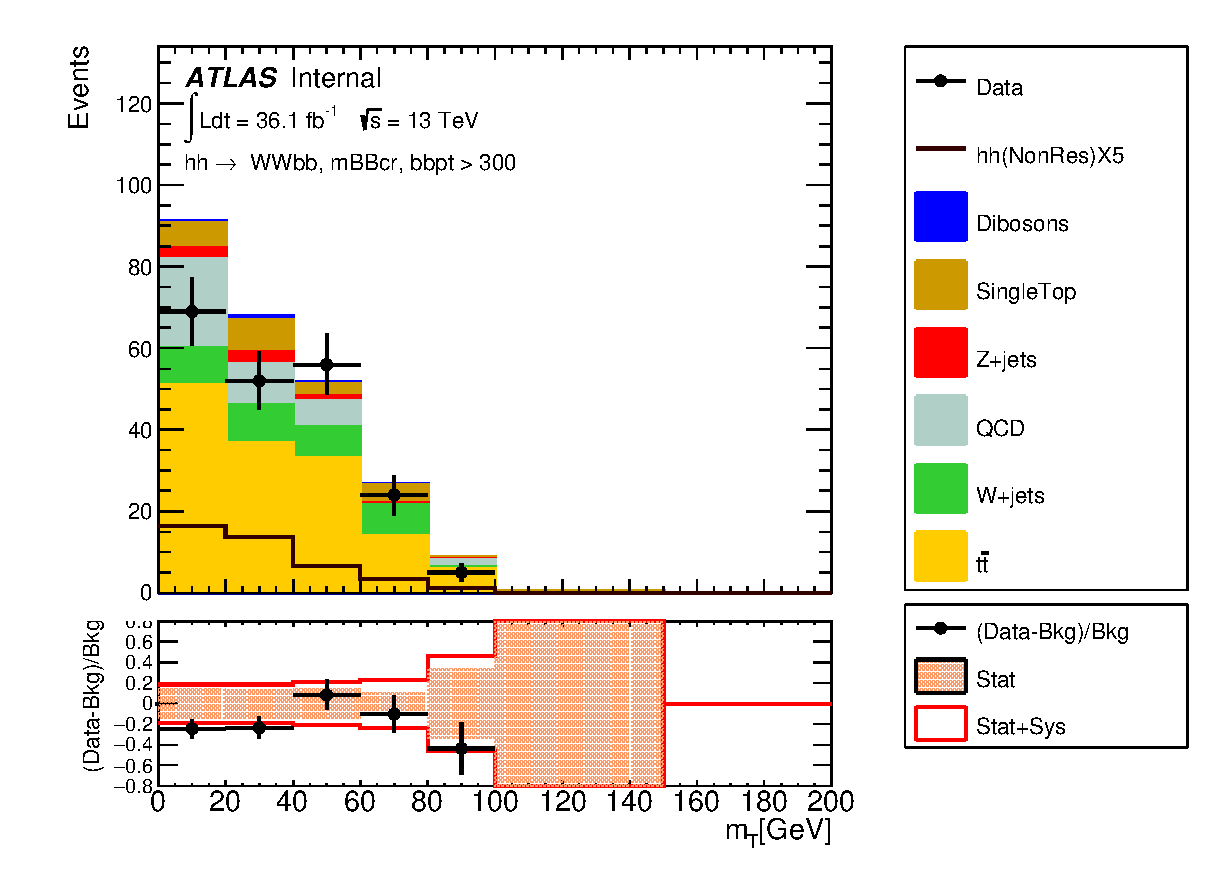
\includegraphics[width=0.45\textwidth, height=0.35\textwidth]{figures/C_reOptNonRes_mww_bbpt210_bbpt300_wlepmtben_regionA_met25d020}
\includegraphics*[width=0.5\textwidth]{paper_figures/C_mBBcr_reOptNonRes_mww_bbpt210_bbpt300_wlepmtben_regionA_met25d020.eps}
%\includegraphics*[width=0.3\textwidth]{figures/C_mBBcr_reOpt500_mww_bbpt210_wlepmtben_regionA_met25d020.eps}
\includegraphics*[width=0.5\textwidth]{paper_figures/C_mBBcr_reOpt700_mww_bbpt210_wlepmtben_regionA_met25d020.eps}
\includegraphics*[width=0.5\textwidth]{paper_figures/C_mBBcr_reOpt2000_bbpt350_wlepmtben_regionA_met25d020.eps}
\caption[The $\mT$ distribution]{The $\mT$ distribution in the three top-background control regions for the \emph{non-res}, \emph{low-mass}, and
 the \emph{high-mass} selections of the resolved analyses.
  %The signal
  %distributions shown are for the  SM non-resonant signal scaled with a factor
  %300 (top-left), and  for the resonant signals with mass 1000~GeV (top-right) and 2000~GeV
  %(bottom) scaled to the expected upper limit cross section reported
  %in Section \ref{sec:MainResults}.
  The signal contamination is negligible, and hence not shown. The lower panel shows the
  fractional difference between the data and the total expected background
  with the corresponding statistical and total uncertainty. }
  \label{fig:resolved_mtlep}
\end{figure}
 
 
Figures~\ref{fig:mbb_1} and ~\ref{fig:mbb_2} show the $m_{b \bar{b}}$ distributions at the
selection stage where all requirements, including the $m_{HH}$ cut, are applied except the one on $m_{b \bar{b}}$ itself.
The expected background is in agreement with the data over the entire distribution, and  
close to the signal region in particular. All simulated backgrounds are normalised according to their theoretical cross-sections, except \ttbar, which is normalised in the top CRs.
 
\begin{figure}
\begin{flushleft}
%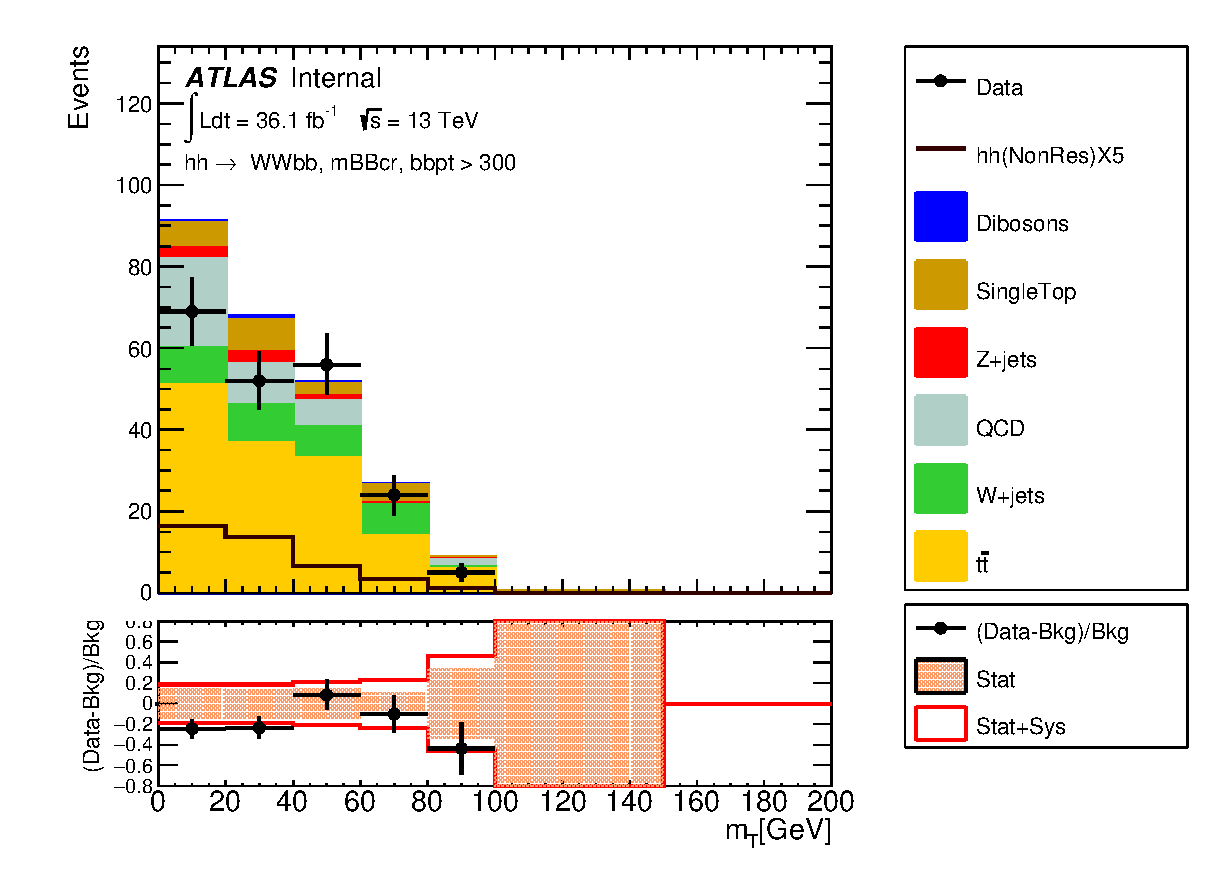
\includegraphics[width=0.45\textwidth, height=0.35\textwidth]{figures/C_reOptNonRes_mww_bbpt210_bbpt300_wlepmtben_regionA_met25d020}
\includegraphics*[width=0.45\textwidth]{paper_figures/C_reOptNonRes_mww_bbpt210_bbpt300_wwpt250_bbMass_regionA_met25d020.eps}
\includegraphics*[width=0.45\textwidth]{paper_figures/C_reOpt500_mww_bbpt210_wwpt150_hh500_bbMass_regionA_met25d020.eps}
\end{flushleft}
\caption[The $m_{b \bar{b}}$ distribution]{The $m_{b \bar{b}}$ distribution in the resolved analysis for the \emph{non-res} and \emph{m500} selections at the end of the
 selection sequence, before applying the $m_{b \bar{b}}$ requirement. The signals shown
 are from SM non-resonant $HH$ production scaled up by a factor of 300 (left) and from a scalar resonance with mass 500~\GeV\ scaled to the expected upper-limit
 cross section reported in Section~\ref{sec:Analysis_results} (right).  The lower panel shows the fractional difference
  between data and the total expected background
 with the corresponding statistical and total uncertainty.
} \label{fig:mbb_1}
\end{figure}
 
\begin{figure}
\begin{flushleft}
\includegraphics*[width=0.45\textwidth]{paper_figures/C_reOpt700_mww_bbpt210_wwpt250_hh1000_bbMass_regionA_met25d020.eps}
\includegraphics*[width=0.45\textwidth]{paper_figures/C_reOpt2000_bbpt350_wwpt250_drww15_hh2000_bbMass_regionA_met25d020.eps}
\end{flushleft}
\caption[The $m_{b \bar{b}}$ distribution]{The $m_{b \bar{b}}$ distribution in the resolved analysis for the
 \emph{low-mass} and \emph{high-mass} selections at the end of the
 selection sequence, before applying the $m_{b \bar{b}}$ requirement. The signals shown
 are from scalar resonances with mass 1000~\GeV\ (left) and 2000~\GeV\ (right)
 scaled to the expected upper-limit cross section reported in
 Section~\ref{sec:Analysis_results}.  The lower panel shows the fractional difference
  between data and the total expected background
 with the corresponding statistical and total uncertainty.} \label{fig:mbb_2}
\end{figure}
 
%\begin{figure}
%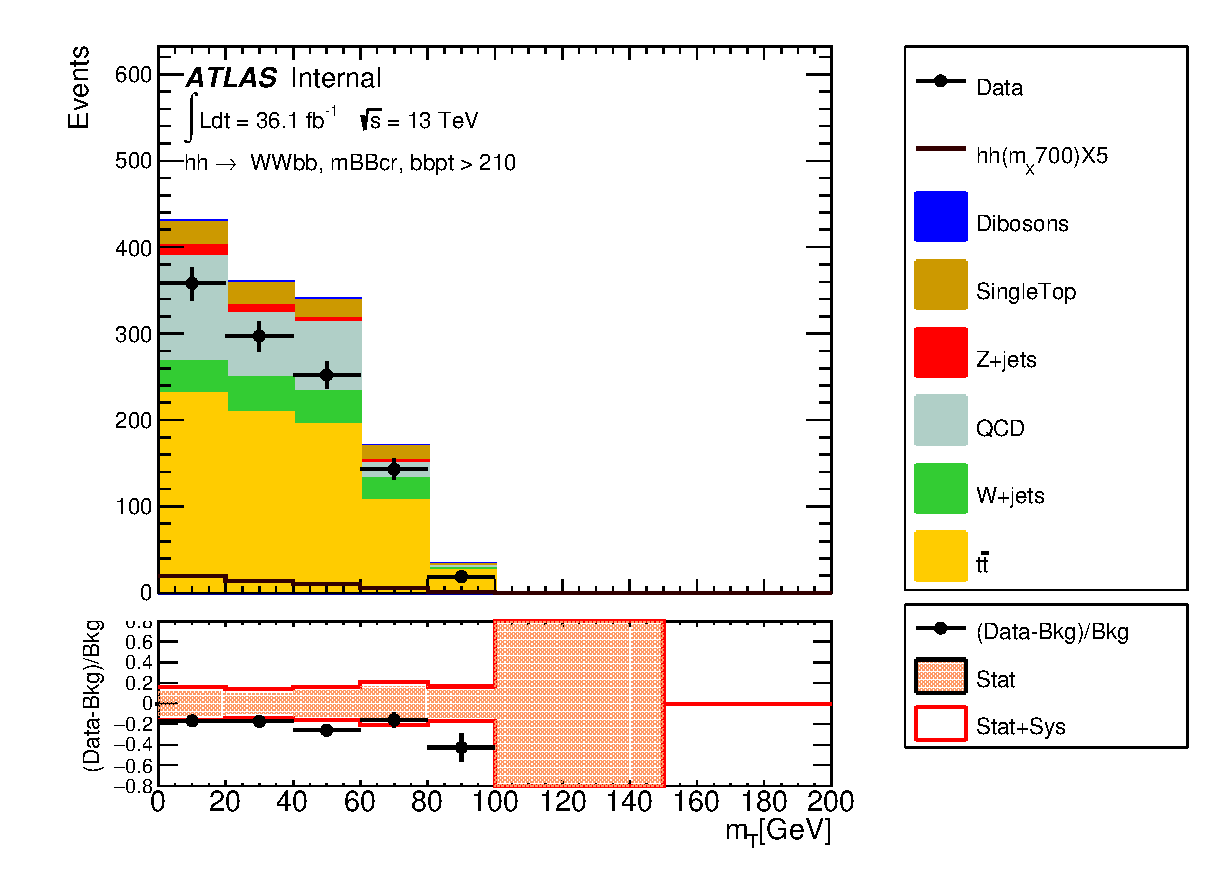
\includegraphics[width=0.45\textwidth, height=0.35\textwidth]{figures/C_reOpt700_mww_bbpt210_wlepmtben_regionA_met25d020}
%\includegraphics*[width=0.45\textwidth]{figures/C_reOpt700_mww_bbpt210_bbMass_regionA_met25d020}
%\caption{$m_{T}$ and $m_{bb}$ distributions for low-mass selection after requiring $p_{T}(bb) > 210$ GeV. The lower panel shows the agreement between data and expected backgrounds and the uncertainties on the total backgrounds. Signal has been arbitrarily scaled to show the shape.}
%\label{fig:mt_mbb_low}
%\end{figure}
 
%\begin{figure}
%\label{fig:mt_mbb_high}
%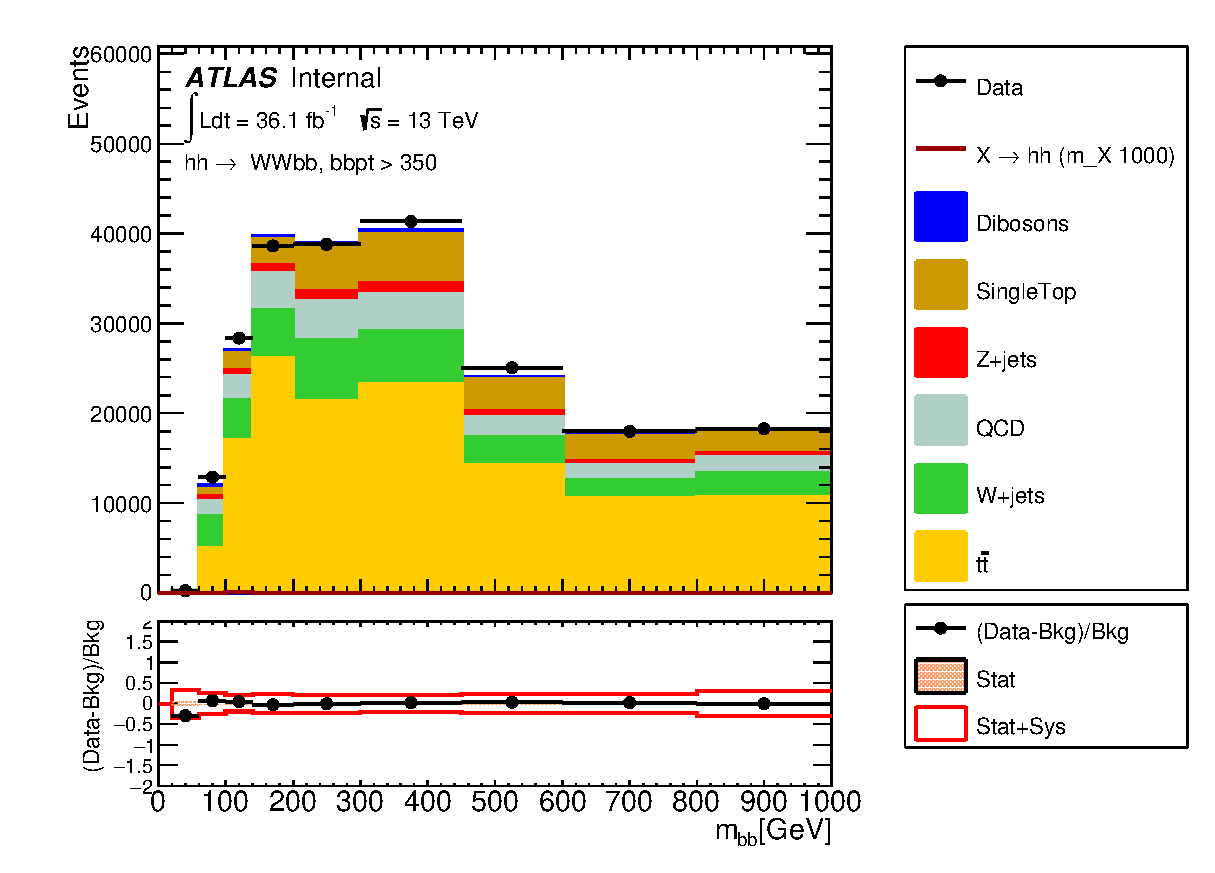
\includegraphics[width=0.45\textwidth, height=0.35\textwidth]{figures/C_reOpt2000_bbpt350_bbMass_regionA_met25d020}
 
%\caption{$m_{T}$ and $m_{bb}$ distributions for high-mass selection after requiring $p_{T}(bb) > 350$ GeV. The lower panel shows the agreement between data and expected backgrounds and the un%certainties on the total backgrounds. Signal has been arbitrarily scaled to show the shape.}
%\end{figure}
 
\begin{table}
%\fontsize{7}{8}\selectfont
 \begin{tabular}{l|c|c|c|c|c}
\hline\hline

\multicolumn{5}{c}{\textbf{SR}: 100 $<$ \mbb $<$ 140 GeV}\\\hline\hline
Sample  	& mww 	& bbpt210 	& bbpt300 	& wwpt250 	& mbb  \\\hline
\ttbar 	& 7461.0 $\pm$ 48.6 	& 162.9 $\pm$ 7.3 	& 27.9 $\pm$ 2.9 	& 18.4 $\pm$ 2.4 	& 15.4 $\pm$ 2.2	\\\hline 
QCD 	& 2756.2 $\pm$ 210.5 	& 48.7 $\pm$ 14.2 	& 6.6 $\pm$ 1.9 	& 4.2 $\pm$ 1.2 	& 3.6 $\pm$ 1.6	\\\hline 
Wv221 	& 640.8 $\pm$ 12.7 	& 19.1 $\pm$ 1.4 	& 5.0 $\pm$ 0.6 	& 3.1 $\pm$ 0.5 	& 2.3 $\pm$ 0.4	\\\hline 
SingleTop 	& 452.2 $\pm$ 9.6 	& 14.3 $\pm$ 1.7 	& 1.7 $\pm$ 0.5 	& 1.0 $\pm$ 0.4 	& 0.6 $\pm$ 0.3	\\\hline 
Dibosonsv221 	& 21.6 $\pm$ 1.3 	& 0.6 $\pm$ 0.2 	& 0.4 $\pm$ 0.2 	& 0.0 $\pm$ 0.0 	& 0.0 $\pm$ 0.0	\\\hline 
Zv221 	& 262.8 $\pm$ 4.4 	& 3.1 $\pm$ 0.3 	& 1.0 $\pm$ 0.2 	& 0.2 $\pm$ 0.1 	& 0.2 $\pm$ 0.1	\\\hline 
\hline
Background Sum 	& 11594.7$\pm$ 216.7 	& 248.6$\pm$ 16.1 	& 42.6$\pm$ 3.6 	& 27.0$\pm$ 2.8 	& 22.1$\pm$ 2.8	\\\hline 
\hline
XhhSM 	& 68.3 $\pm$ 2.4 	& 20.7 $\pm$ 0.9 	& 6.7 $\pm$ 0.4 	& 5.5 $\pm$ 0.3 	& 4.8 $\pm$ 0.3	\\\hline 
Data 	& 11450.0 	& 232.0 	& 47.0 	& 31.0 	& 22.0	\\\hline 
\end{tabular}
\caption[Number of SR events in the non-res selection]{ The number of expected background and signal events in the
  $m_{bb}$ SR for the non-resonant selection. Only statistical uncertainties are shown. No NF has been applied.} 
\label{tab:nonresSRyields}
\end{table}

%%%%%%%%%%%%%%%%%%%
\begin{center}
\begin{table}
%\fontsize{7}{8}\selectfont
\begin{tabular}{l|c|c|c|c|c}
\hline\hline
\multicolumn{5}{c}{\textbf{SR}: 100 $<$ \mbb $<$ 140 GeV}\\\hline\hline
Sample  	& mww 	& bbpt210 	& wwpt150 	& hh500 	& mbb  \\\hline
\ttbar 	& 7461.0 $\pm$ 48.6 	& 162.9 $\pm$ 7.3 	& 141.7 $\pm$ 6.8 	& 17.3 $\pm$ 2.2 	& 12.6 $\pm$ 1.9	\\\hline 
QCD 	& 2756.2 $\pm$ 210.5 	& 48.7 $\pm$ 14.2 	& 40.2 $\pm$ 11.7 	& 3.3 $\pm$ 1.0 	& 2.9 $\pm$ 1.3	\\\hline 
Wv221 	& 640.8 $\pm$ 12.7 	& 19.1 $\pm$ 1.4 	& 15.3 $\pm$ 1.3 	& 0.1 $\pm$ 0.0 	& -0.2 $\pm$ 0.1	\\\hline 
SingleTop 	& 452.2 $\pm$ 9.6 	& 14.3 $\pm$ 1.7 	& 12.2 $\pm$ 1.6 	& 3.6 $\pm$ 0.8 	& 2.8 $\pm$ 0.7	\\\hline 
Dibosonsv221 	& 21.6 $\pm$ 1.3 	& 0.6 $\pm$ 0.2 	& 0.5 $\pm$ 0.2 	& 0.1 $\pm$ 0.0 	& 0.1 $\pm$ 0.0	\\\hline 
Zv221 	& 262.8 $\pm$ 4.4 	& 3.1 $\pm$ 0.3 	& 1.9 $\pm$ 0.2 	& 0.5 $\pm$ 0.1 	& 0.4 $\pm$ 0.1	\\\hline 
\hline
Background Sum 	& 11594.7$\pm$ 216.7 	& 248.6$\pm$ 16.1 	& 211.8$\pm$ 13.7 	& 24.9$\pm$ 2.5 	& 18.6$\pm$ 2.4	\\\hline 
\hline
Xhh500 	& 6.6 $\pm$ 0.2 	& 1.9 $\pm$ 0.1 	& 1.7 $\pm$ 0.1 	& 0.9 $\pm$ 0.1 	& 0.8 $\pm$ 0.1	\\\hline 
Data 	& 11450.0 	& 232.0 	& 194.0 	& 32.0 	& 26.0	\\\hline 
\end{tabular}
\caption[Number of SR events in the m500 selection]{ The number of expected background and signal events in the  $m_{bb}$ SR for the low-mass selection, m500. Only statistical uncertainties are shown. No NF has been applied.} 
\end{table}
\end{center}


%%%%%%%%%%%%%%%%

\begin{center}
\begin{table}
%\fontsize{7}{8}\selectfont
\begin{tabular}{l|c|c|c|c|c}
\hline\hline
\multicolumn{5}{c}{\textbf{CR}: \mbb Sideband}\\\hline\hline
\multicolumn{5}{c}{\textbf{SR}: 100 $<$ \mbb $<$ 140 GeV}\\\hline\hline
Sample  	& mww 	& bbpt210 	& wwpt250 	& hh700 	& mbb  \\\hline
\ttbar 	& 7461.0 $\pm$ 48.6 	& 162.9 $\pm$ 7.3 	& 61.5 $\pm$ 4.7 	& 21.9 $\pm$ 2.7 	& 15.3 $\pm$ 2.2	\\\hline 
QCD 	& 2756.2 $\pm$ 210.5 	& 48.7 $\pm$ 14.2 	& 14.1 $\pm$ 4.1 	& 5.5 $\pm$ 1.6 	& 4.8 $\pm$ 2.2	\\\hline 
Wv221 	& 640.8 $\pm$ 12.7 	& 19.1 $\pm$ 1.4 	& 9.7 $\pm$ 1.1 	& 4.1 $\pm$ 0.8 	& 2.6 $\pm$ 0.6	\\\hline 
SingleTop 	& 452.2 $\pm$ 9.6 	& 14.3 $\pm$ 1.7 	& 2.6 $\pm$ 0.7 	& 0.5 $\pm$ 0.2 	& 0.3 $\pm$ 0.2	\\\hline 
Dibosonsv221 	& 21.6 $\pm$ 1.3 	& 0.6 $\pm$ 0.2 	& 0.2 $\pm$ 0.1 	& 0.2 $\pm$ 0.1 	& 0.2 $\pm$ 0.1	\\\hline 
Zv221 	& 262.8 $\pm$ 4.4 	& 3.1 $\pm$ 0.3 	& 0.6 $\pm$ 0.1 	& 0.1 $\pm$ 0.0 	& 0.1 $\pm$ 0.0	\\\hline 
\hline
Background Sum 	& 11594.7$\pm$ 216.7 	& 248.6$\pm$ 16.1 	& 88.7$\pm$ 6.4 	& 32.3$\pm$ 3.2 	& 23.3$\pm$ 3.1	\\\hline 
\hline
Xhh700 	& 9.2 $\pm$ 0.3 	& 7.8 $\pm$ 0.2 	& 5.9 $\pm$ 0.2 	& 5.0 $\pm$ 0.2 	& 4.4 $\pm$ 0.2	\\\hline 
Data 	& 11450.0 	& 232.0 	& 75.0 	& 25.0 	& 22.0	\\\hline 
\end{tabular}
\caption[Number of SR events in the m700 selection]{ The number of expected background and signal events in the  $m_{bb}$ SR for the low-mass selection, m700. Only statistical uncertainties are shown. No NF has been applied.} 
\end{table}
\end{center}

%%%%%%%%%%%%%%%

\begin{center}
\begin{table}
%\fontsize{7}{8}\selectfont
\begin{tabular}{l|c|c|c|c|c}
\hline\hline
\multicolumn{5}{c}{\textbf{SR}: 100 $<$ \mbb $<$ 140 GeV}\\\hline\hline
Sample  	& bbpt350 	& wwpt250 	& drww15 	& hh2000 	& mbb  \\\hline
\ttbar 	& 1307.8 $\pm$ 20.2 	& 1024.9 $\pm$ 17.7 	& 287.5 $\pm$ 9.4 	& 2.2 $\pm$ 0.8 	& 1.4 $\pm$ 0.6	\\\hline 
QCD 	& 207.2 $\pm$ 99.5 	& 191.2 $\pm$ 29.0 	& 55.2 $\pm$ 8.4 	& 2.9 $\pm$ 0.4 	& 2.2 $\pm$ 0.5	\\\hline 
Wv221 	& 341.3 $\pm$ 3.4 	& 291.5 $\pm$ 3.2 	& 110.7 $\pm$ 2.1 	& 4.8 $\pm$ 0.3 	& 3.4 $\pm$ 0.3	\\\hline 
SingleTop 	& 144.1 $\pm$ 5.6 	& 126.6 $\pm$ 5.3 	& 29.2 $\pm$ 2.6 	& 0.5 $\pm$ 0.3 	& 0.5 $\pm$ 0.3	\\\hline 
Dibosonsv221 	& 25.9 $\pm$ 1.5 	& 21.8 $\pm$ 1.3 	& 6.6 $\pm$ 0.7 	& 0.0 $\pm$ 0.0 	& 0.0 $\pm$ 0.0	\\\hline 
Zv221 	& 53.8 $\pm$ 0.8 	& 40.4 $\pm$ 0.7 	& 13.2 $\pm$ 0.4 	& 0.8 $\pm$ 0.1 	& 0.7 $\pm$ 0.1	\\\hline 
\hline
Background Sum 	& 2080.1$\pm$ 101.8 	& 1696.5$\pm$ 34.6 	& 502.5$\pm$ 13.1 	& 11.2$\pm$ 1.0 	& 8.2$\pm$ 0.8	\\\hline 
\hline
Xhh2000 	& 21.0 $\pm$ 0.4 	& 19.3 $\pm$ 0.4 	& 8.4 $\pm$ 0.2 	& 3.4 $\pm$ 0.1 	& 2.9 $\pm$ 0.1	\\\hline 
Data 	& 2182.0 	& 1830.0 	& 587.0 	& 11.0 	& 9.0	\\\hline
\end{tabular}
\caption[Number of SR events in the m2000 selection]{ The number of expected background and signal events in the  $m_{bb}$ SR for the high-mass selection, m2000. Only statistical uncertainties are shown. No NF has been applied.} 
\label{tab:highmassSRyields}
\end{table}
\end{center}

\subsection{Systematic Uncertainties}
This section describes the sources of systematic uncertainties
considered in the analysis. These uncertainties are divided into four
categories: experimental uncertainties, uncertainties on the data
driven background estimation,  uncertainties on the modelling
of background processes estimated from simulation, theoretical
uncertainties on the signal processes. In the statistical analysis
each systematic uncertainty is treated as a nuisance parameter the
names of which are defined below. These systematic variations are
estimated on the final expected yield in the signal regions.

\subsection{Experimental uncertainties}

Each reconstructed object has several sources of uncertainties, each
of which are evaluated separately. Wherever possible, we follow the
latest available recommendations from the combined performance (CP)
groups. The leading instrumental uncertainties are
the uncertainty on the $b$-tagging efficiency and the jet energy scale
(JES). The summary of experimental uncertainties is presented in
Table~\ref{tab:syst_summary_sources}.
 
\begin{table}[h]
\centering
\small
\scriptsize
\begin{center}
\begin{tabular}{|l|l|l|l|}
\hline
Source        & Description                          & Analysis Name                         \\ 
\hline
%Muons         & Trigger                                 &    Muons\_Trig                              \\
Muons         & \pt resolution MS                 &   MUON\_MS                           \\ 
Muons         & \pt resolution ID                   &   MUON\_ID                             \\ 
Muons         & \pt scale                               &   MUON\_SCALE                     \\ 
Muons         & Isolation efficiency SF         &   MUON\_ISO\_SYS               \\ 
Muons         & Isolation efficiency SF         &   MUON\_ISO\_STAT              \\ 
Muons         & Reconstruction efficiency SF         &  MUON\_EFF\_SYS             \\ 
Muons         & Reconstruction efficiency SF         &  MUON\_EFF\_STAT           \\ 
Muons         & Trigger efficiency SF            &  MUON\_EFF\_TrigStatUncertainty \\ 
Muons         & Trigger efficiency SF            &  MUON\_EFF\_TrigSystUncertainty  \\ 
%Muons         & TTVA efficiency SF         &   MUON\_TTVA\_SYS              & \\ 
%Muons         & TTVA efficiency SF         &   MUON\_TTVA\_STAT             & \\ 
\hline
Electrons         & \pt resolution                           &   EG\_RESOLUTION\_ALL       \\ 
Electrons         & \pt scale                                  &   EG\_SCALE\_ALL                   \\ 
Electrons         & Isolation efficiency SF             &   EL\_EFF\_Iso\_TOTAL\_1NPCOR\_PLUS\_UNCOR  \\ 
Electrons         & Reconstruction efficiency SF  &   EL\_EFF\_Reco\_TOTAL\_1NPCOR\_PLUS\_UNCOR  \\ 
Electrons         & Trigger efficiency SF               &   EL\_EFF\_Trigger\_TOTAL\_1NPCOR\_PLUS\_UNCOR  \\ 
Electrons         & Identification efficiency SF      &   EL\_EFF\_ID\_TOTAL\_1NPCOR\_PLUS\_UNCOR  \\ 
\hline
Tau	               & Energy scale model			& TAUS\_TRUEHADTAU\_SME\_TES\_MODEL\\
Tau	               & Energy scale detector		& TAUS\_TRUEHADTAU\_SME\_TES\_DETECTOR \\
Tau	               & In-situ energy calibration		& TAUS\_TRUEHADTAU\_SME\_TES\_INSITU \\
\hline
MET           & Soft term                       &   MET\_SoftTrk\_ResoPerp            \\ 
MET           & Soft term                       &   MET\_SoftTrk\_ResoPara            \\ 
MET           & Soft term                       &   MET\_SoftTrk\_Scale              \\ 
\hline
Small-R Jets  & JES strongly reduced            &   JET\_SR1\_JET\_GroupedNP\_1                   \\ 
Small-R Jets  & JES strongly reduced            &   JET\_SR1\_JET\_GroupedNP\_2                   \\ 
Small-R Jets  & JES strongly reduced            &   JET\_SR1\_JET\_GroupedNP\_3                   \\ 
Small-R Jets  & JES strongly reduced            &   JET\_SR1\_JET\_EtaIntercalibration\_NonClosure  \\ 
Small-R Jets  & Energy resolution                  &   JET\_JER\_SINGLE\_NP                               \\ 
Small-R Jets  & JVT efficiency SF                  &   JET\_JvtEfficiency                                                   \\ 
\hline
$b$-tagging     & Flavor tagging scale factors    &    FT\_EFF\_Eigen\_Light\_0                               \\
$b$-tagging     & Flavor tagging scale factors    &    FT\_EFF\_Eigen\_Light\_1                               \\
$b$-tagging     & Flavor tagging scale factors    &    FT\_EFF\_Eigen\_Light\_2                               \\
$b$-tagging     & Flavor tagging scale factors    &    FT\_EFF\_Eigen\_Light\_3                               \\
$b$-tagging     & Flavor tagging scale factors    &    FT\_EFF\_Eigen\_Light\_4                               \\
$b$-tagging     & Flavor tagging scale factors    &    FT\_EFF\_Eigen\_Light\_5                               \\
$b$-tagging     & Flavor tagging scale factors    &    FT\_EFF\_Eigen\_Light\_6                               \\
$b$-tagging     & Flavor tagging scale factors    &    FT\_EFF\_Eigen\_Light\_7                               \\
$b$-tagging     & Flavor tagging scale factors    &    FT\_EFF\_Eigen\_Light\_8                               \\
$b$-tagging     & Flavor tagging scale factors    &    FT\_EFF\_Eigen\_Light\_9                               \\
$b$-tagging     & Flavor tagging scale factors    &    FT\_EFF\_Eigen\_Light\_10                             \\
$b$-tagging     & Flavor tagging scale factors    &    FT\_EFF\_Eigen\_Light\_11                             \\
$b$-tagging     & Flavor tagging scale factors    &    FT\_EFF\_Eigen\_Light\_12                             \\
$b$-tagging     & Flavor tagging scale factors    &    FT\_EFF\_Eigen\_Light\_13                             \\
$b$-tagging     & Flavor tagging scale factors    &    FT\_EFF\_Eigen\_B\_0                               \\
$b$-tagging     & Flavor tagging scale factors    &    FT\_EFF\_Eigen\_B\_1                               \\
$b$-tagging     & Flavor tagging scale factors    &    FT\_EFF\_Eigen\_B\_2                               \\
$b$-tagging     & Flavor tagging scale factors    &    FT\_EFF\_Eigen\_B\_3                               \\
$b$-tagging     & Flavor tagging scale factors    &    FT\_EFF\_Eigen\_B\_4                               \\
$b$-tagging     & Flavor tagging scale factors    &    FT\_EFF\_Eigen\_C\_0                              \\
$b$-tagging     & Flavor tagging scale factors    &    FT\_EFF\_Eigen\_C\_1                               \\
$b$-tagging     & Flavor tagging scale factors    &    FT\_EFF\_Eigen\_C\_2                               \\
$b$-tagging     & Flavor tagging scale factors    &    FT\_EFF\_Eigen\_C\_3                               \\
$b$-tagging     & Flavor tagging scale factors    &    FT\_EFF\_Eigen\_C\_4                               \\
$b$-tagging     & Flavor tagging scale factors    &    FT\_EFF\_Eigen\_extrapolation                           \\
$b$-tagging     & Flavor tagging scale factors    &   FT\_EFF\_Eigen\_extrapolation\_from\_charm     \\
\hline
\hline
\end{tabular}
\caption[Object systematic uncertainties]{ Qualitative summary of the object systematic uncertainties included in this analysis.}
\label{tab:syst_summary_sources}
\end{center}
\end{table}

 
 
 \iffalse
\begin{table}[h]
\centering
\small
\begin{center}
\begin{tabular}{|l|l|l|}
\hline
Source        & Description                     & Analysis Name
  \\ \hline
Muons          & Trigger      & Muons\_Trig \\
Muons         & \pt resolution MS               &   MUONS\_MS                          \\ 
Muons         & \pt resolution ID               &   MUONS\_ID                           \\ 
Muons         & \pt scale                       &   MUONS\_SCALE                        \\ 
Muons         & Isolation efficiency SF         &   MUON\_ISO\_SYS                      \\ 
Muons         & Isolation efficiency SF         &   MUON\_ISO\_STAT                     \\ 
Muons         & Identification efficiency SF    &   MUON\_EFF\_SYS                      \\ 
Muons         & Identification efficiency SF    &   MUON\_EFF\_STAT                     \\ \hline
MET           & Soft term                       &   MET\_SoftTrk\_ResoPerp              \\ 
MET           & Soft term                       &   MET\_SoftTrk\_ResoPara              \\ 
MET           & Soft term                       &   MET\_SoftTrk\_ScaleUp               \\ \hline
Small-R Jets  & JES strongly reduced            &   JET\_GroupedNP\_1                   \\ 
Small-R Jets  & JES strongly reduced            &   JET\_GroupedNP\_2                   \\ 
Small-R Jets  & JES strongly reduced            &   JET\_GroupedNP\_3                   \\ 
Small-R Jets  & Energy resolution               &   JET\_JER\_SINGLE\_NP                \\ \hline
$b$-tagging     & Flavor tagging scale factors    &    FT\_EFF\_Eigen\_Light0                               \\
$b$-tagging     & Flavor tagging scale factors    &    FT\_EFF\_Eigen\_Light1                               \\
$b$-tagging     & Flavor tagging scale factors    &    FT\_EFF\_Eigen\_Light2                               \\
$b$-tagging     & Flavor tagging scale factors    &    FT\_EFF\_Eigen\_Light3                               \\
$b$-tagging     & Flavor tagging scale factors    &    FT\_EFF\_Eigen\_Light4                               \\
$b$-tagging     & Flavor tagging scale factors    &    FT\_EFF\_Eigen\_B0                               \\
$b$-tagging     & Flavor tagging scale factors    &    FT\_EFF\_Eigen\_B1                               \\
$b$-tagging     & Flavor tagging scale factors    &    FT\_EFF\_Eigen\_B2                               \\
$b$-tagging     & Flavor tagging scale factors    &    FT\_EFF\_Eigen\_C0                               \\
$b$-tagging     & Flavor tagging scale factors    &    FT\_EFF\_Eigen\_C1                               \\
$b$-tagging     & Flavor tagging scale factors    &    FT\_EFF\_Eigen\_C2                               \\
$b$-tagging     & Flavor tagging scale factors    &    FT\_EFF\_Eigen\_C3                               \\
$b$-tagging     & Flavor tagging scale factors    &    FT\_EFF\_Eigen\_extrapolation                               \\
$b$-tagging     & Flavor tagging scale factors    &   FT\_EFF\_Eigen\_extrapolation\_from\_charm                               \\
\hline
Modelling      & $t\bar{t}$ ME              & Matching &       TopMCaNLOtt    \\ 
Modelling      & $t\bar{t}$ Scale             &      ScaleVariation  & Top\_Scale      \\ 
Modelling      & $t\bar{t}$ PDF             &    PDFVariation &    Top\_PDF     \\ 
Modelling      & $t\bar{t}$ PS               & Parton Shower &       Top\_PS    \\ 
\hline
\end{tabular}
\caption{ Qualitative summary of the systematic uncertainties included in this analysis. }
\label{tab:syst_summary_sources}
\end{center}
\end{table}
\fi

\clearpage

\subsubsection{Luminosity}
The uncertainty in the combined 2015+2016 integrated luminosity is 2.1\%\footnote{\url{https://twiki.cern.ch/twiki/bin/view/Atlas/LuminosityForPhysics}}. It is derived, following a methodology similar to that detailed in ~\cite{Aaboud:2016hhf}, from a preliminary calibration of the luminosity scale using x-y beam-separation scans performed in August 2015 and May 2016. The luminosity uncertainty is applied to those backgrounds estimated from simulation and the signal samples.

\subsubsection{Trigger}
Systematic uncertainties on the efficiency of electron and muon triggers are
evaluated as recommended by the corresponding combined performance groups as documented here.\footnote{el: \url{https://twiki.cern.ch/twiki/bin/viewauth/AtlasProtected/ElectronEfficiencyRun2} \\ mu:\url{https://twiki.cern.ch/twiki/bin/view/AtlasProtected/MCPAnalysisGuidelinesMC15}} 

\subsubsection{Muons}
The following systematic uncertainties are applied to muons in estimations based on the simulation:

\begin{itemize}
\item Identification efficiency: The efficiencies are measured with the tag and probe method using the $Z$ mass peak.
\item Energy and Momentum scales: These are also measured with $Z$ mass line shape, and provided by the CP groups. 
\end{itemize}

\subsubsection{Electrons}

The following systematic uncertainties are applied to electron in estimations based on the simulation:

\begin{itemize}
\item Identification efficiency: The efficiencies are measured with
  the tag and probe method using the $Z$ mass peak. They include
  contributions from reconstruction, identification and isolation;
\item Energy and Momentum scales: These are also measured with $Z$ mass line shape, and provided by the CP groups. 
\end{itemize}

\subsubsection{Jet uncertainties}
The jet energy uncertainties are derived based on in situ measurements
performed during Run 2 conditions ~~\cite{ATL-PHYS-PUB-2015-015}. The jet energy
resolution uncertainty is evaluated by smearing jet energies according
to the systematic uncertainties of the resolution
measurement~~\cite{Aad:2014bia}. The uncertainty in the $b$-tagging
efficiency is evaluated by propagating the systematic uncertainty in
the measured tagging efficiency for
$b$-jets~~\cite{ATLAS-CONF-2014-004}. The ``Loose'' reduction scheme
is used.


\subsubsection{Missing transverse energy}
The systematic uncertainties related to the missing transverse energy
are obtained by the propagation of the systematic uncertainty on the
objects that build the MET, in particular the muon, electron and jets
energy resolution and scale. 
The resolution and scale of the MET soft-term is broken down into its components: METScale, METResoPara, METResoPerp, and full uncertainties from each component is taken into account in the final fit. 
 
% ($|d_{0}^{\textrm{sig}}| = d_{0}/\sigma{_{\textrm{d_{0}}}}$)
\subsubsection{$d_{0}^{\textrm{sig}}$ uncertainties}
The uncertainty due to the $d_{0}^{\textrm{sig}}$ cut has been evaluated by making the ratio between the efficiency of the cut for data and the efficiency of the cut for the MC background samples. 
We selected di-electron or di-muon event, requiring an invariant di-leptons mass within 80-100 GeV Z Mass window. To be as similar to our signal region as possible but to keep high statistics, loose pre-selection cuts are applied in selecting the events. The leading lepton is required to have $\pt > 27$~GeV and $\met > 25$~GeV. At least 4 resolved jets are required of which exactly 2 are $b$-jets. 
The $d_{0}^{\textrm{sig}}$ distributions for data and MC samples for each lepton channel are shown in the Figure~\ref{fig:d0lep}, in Figure~\ref{fig:d0ratio} the relative ratio of the total distributions is shown.
The ratio of the efficiency of the $d_{0}^{\textrm{sig}}$ cut for data over MC samples si about 96\%, this is equivalent if the ratio is estimated by using only muons or only electrons. 
The difference of this ratio from one is the fractional uncertainty due to the $d_{0}^{\textrm{sig}}$ cut efficiency.


%\begin{equation}                                                                                                                          
%$\{Uncertainty}_{\sigma_{d_0}~cut}= {\frac{\epsilon_{\sigma_{d_0}~cut}}_{DATA}}{{\epsilon_{\sigma_{d_0}~cut}_{MC}}}$                      
%$\epsilon_{\sigma_{d_0}~cut}= \frac{N~passing~\sigma_{d_0}\le2.0}{N~Total}$                                                               
%\end{equation}                                                                                                                            
This results in about 4\% for the $d_{0}^{\textrm{sig}}$ uncertainty independent from the lepton flavour.
\begin{figure}[!h]
\begin{center}
\includegraphics*[width=0.47\textwidth] {figures/d0_data}
\includegraphics*[width=0.47\textwidth] {figures/do_leg}
\caption{$d_{0}^{\textrm{sig}}$ distributions for data and background MC samples, identifying the lepton channel. }
\label{fig:d0lep}
\end{center}
\end{figure}

\begin{figure}[!h]
\begin{center}
\includegraphics*[width=0.6\textwidth] {figures/d0_ratio}
\caption{$d_{0}^{\textrm{sig}}$ distributions and the relative ratio for data and background MC samples. }
\label{fig:d0ratio}
\end{center}
\end{figure}


\subsection{Background modelling uncertainties}
Several systematics have been evaluated to take into account the
uncertainties on the modelling of backgrounds. 

\subsubsection{Uncertainties from the modelling of $t\bar{t}$}
\label{sec:topsys}
The dominant background $t\bar{t}$ is normalised in dedicated CRs. MC is used to extrapolate the shapes from the control regions to the signal region, so theoretical uncertainties are related to such extrapolation. PDF and scale uncertainties are evaluated by applying event selection at truth level. The resulting uncertainties are approximately 5 to 6\% and are included in the final fit.  

Additional uncertainties in $t\bar{t}$ modelling stems from the difference in the matrix element (ME) implementation across generators, hadronisation and fragmentation modelling (called parton shower, PS), and the amount of initial and final state radiation (ISR/FSR). The ME uncertainty is computed by comparing the events generated by \textsc{aMC@NLO} with the events generated by \textsc{Powheg-Box} v2, both interfaced to \textsc{Herwig++}  for parton shower. The difference computed close to the signal region with enough statistics is used. The PS uncertainty is computed by comparing the the nominal \textsc{Powheg+Pythia6} sample with the PS variation \textsc{Powheg+Herwig++} sample in a region close to the SR but with enough statistics. For ISR/FSR, the dedicated \textsc{radHi} and \textsc{radLo} samples with modified \textsc{hDamp} parameter are compared. The sample with the higher impact on the fit is kept as the uncertainty due to ISR/FSR. Table~\ref{tab:ttbarModeling} shows the numbers provided to the fit for the various \ttbar modelling systematics for the low and high mass selections. Since the uncertainties are computed based on extrapolation from the CRs, these uncertainties are input to the statistical fit as rate uncertainties in the SR only. 

\begin{table}
\centering
\begin{tabular}{l|ccc}
\hline
Source               & Non-resonant 	&  Low-Mass   		& 		High-Mass   \\\hline\hline 
Matrix Element       & 7.2 			&    0.5                	 &           	4.1                 \\\hline
Parton Shower        & 3.7 			&   16.4                     &              9.5                 \\\hline
ISR/FSR              & 14.7 			&  4.9       			 &             8.2                 \\\hline
PDF                  & 5.2 			&  3.5 			&           6.1                 \\\hline
Scale                & 3.3 			& 2.2                		&               3.7                 \\\hline\hline

\end{tabular}
\caption[Extrapolation uncertainties]{Extrapolation uncertainties in percentage from the CR to the SR for all selections,  provided to the fit for the \ttbar modelling systematics.}
\label{tab:ttbarModeling}
\end{table}



\iffalse
An uncertainty on the shape of the $m_{hh}$  for $t\bar{t}$ is derived
comparing  the default Powheg+Herwig++ sample with the distribution obtained
using aMC@NLO+Heriwg++ as alternative generator. Additional systematic
uncertainties are evaluated by comparing the nominal sample showered
with Pythia to one showered with Herwig++. Sample with renormalisation
and factorisation scales doubled
and halved are also available and used as systematic uncertainty. 
The Samples used for the systematic uncertainties are the following:

\begin{itemize}
\item mc15\_13TeV.410000.PowhegPythiaEvtGen\_P2012\_ttbar\_hdamp172p5\_nonallhad - Nominal
\item mc15\_13TeV.410003.aMcAtNloHerwigppEvtGen\_ttbar\_nonallhad - TTBarMCNLO
\item mc15\_13TeV.410004.PowhegHerwigppEvtGen\_UEEE5\_ttbar\_hdamp172p5\_nonallhad - TTBarHerwig
\end{itemize}
\fi

\subsubsection{Single top uncertainty}
Theoretical cross section uncertainties of 5.3\% is assigned to the associated $Wt$ production,  3.9\% to the s-channel and 4.2\% to t-channel single top production.  The dominant production for this analysis is the $Wt$ channel.  The single top modelling systematic uncertainties have been calculated employing the difference between the nominal (DR scheme) and the (available) systematic variation sample (DS scheme) in SR for the $Wt$ channel. The uncertainties are computed to be 48\%, 48\%, and 84\% for non-resonant, low-mass and high-mass analyses respectively.  Single top is a very small background in the analysis. However, the large difference between the two schemes warranted getting feedback from the Top Group. We narrowed the huge difference down to very tight $p_{T} (bb)$ cut. See Figure~\ref{fig:stop_bbpt}. The Top Group is working on a better prescription but in the meantime this is the recommended method and the huge difference is what we keep. 
Additional uncertainties on single top have been calculated employing the difference between the nominal and the (available) systematic variation samples. The recommendation is taken from the Top Twiki.{\footnote {\url{https://twiki.cern.ch/twiki/bin/viewauth/AtlasProtected/TopSystematics2015}}} 
The comparison is done between the nominal sample and the Powheg+Herwig for fragmentation, MC@NLO for Matrix Element, and RadHi/RadLo for ISR/FSR uncertainties. The comparison is done at the selection where MC statistical uncertainties are small. This leads to $p_{T}(bb) < 120$ for non-resonance and low-mass selections, and $\Delta R(WW) < 1.5$ for high-mass selection. 
The uncertainties vary across selections being 3.5\% at the smallest to 23\% at the largest.% Appendix~\ref{app:app_stop_unc} provides detailed tables of the comparison of nominal with alternative single top samples. 

\begin{figure}[!h]
\begin{center}
\includegraphics*[width=0.47\textwidth] {figures/DR_DS_bbpt.eps}
\caption[$p_{T}(bb)$  for DR and DS schemes for single top modelling.]{$p_{T}(bb)$  for DR and DS schemes for single top modelling.}
\label{fig:stop_bbpt}
\end{center}
\end{figure}

%The recommendation is taken from the Top Twiki.{\footnote {\url{https://twiki.cern.ch/twiki/bin/viewauth/AtlasProtected/TopSystematics2015}}} 
%The uncertainties vary across Wt, t, and s channels , and for low mass versus high mass selection. At the smallest it is 3.9\% and at the largest 67\%. To avoid too many nuisance parameters, we have added them in quadrature and now use the following: For Low Mass, 16\% in CR and 34\% in SR. For high mass, 66\% in CR and 69\% in SR.


\subsubsection{$W/Z$+jets modelling uncertainty}
\label{sec:WjetsModeling}
Uncertainties on the modelling of $W$+jets background were computed in
each SR and top CR. Three sources of uncertainties were considered:
scale variation uncertainties, PDF uncertainties and PS/modelling
uncertainties. Scale uncertainties were computed by varying by a
factor 2 the nominal renormalisation and factorisation scales, PDF
uncertainties were computed according to the NNPDF recipe, that is
computing the standard deviation of the 100 PDF eigenset, while
modelling uncertainties were computed comparing Sherpa with
Alpgen+Pythia6. The values obtained in each region are
summarised in Table \ref{tab:wplusjet_uncertainties}. Same
uncertainties are used for the subleading $Z$+jets background.
\begin{table}
\centering
\begin{tabular}{l|cc|cc|cc}
\hline
Source               &\multicolumn{2}{c} {Non-resonant} 	& \multicolumn{2}{c}{Low-Mass}   		& \multicolumn{2}{c}{High-Mass}   \\\hline\hline 
\hline
& SR & CR & SR & CR & SR & CR \\
\hline

Modelling/PS       & 37 & 37 	&   37 & 37 &  18 & 18             \\\hline
PDF                  & 7 & 30 	&  10 & 36 & 17 & 31         \\\hline
Scale                & 25 & 35 & 17 & 31 & 29 & 28      \\\hline\hline
\end{tabular}
\caption[Theoretical uncertainties in percentage on $W/Z$+jets event
  yield]{Theoretical uncertainties in percentage on $W/Z$+jets event
  yield computed in the CR  and the  SR of all selections,  provided
  to the fit for the W/Z jets modelling systematics.}

\label{tab:wplusjet_uncertainties}
\end{table}


\subsubsection{QCD uncertainty}
An overall 36\% uncertainty is assigned to the QCD multijet background. The systematic uncertainty was calculated following the steps described in Section~\ref{sec:multijet}. 


\subsection{Model uncertainties on the signal}

Systematics on signal acceptance are computed generating
multiple-weight samples that include weights corresponding to
variation of the normalisation and factorisation scales by a factor
$(\xi_r, \xi_f)= 2$. The envelope is built excluding the cases where
$\xi_r/\xi_f = 4$ and $\xi_r/\xi_f = 1/4$. The fractional uncertainty
is obtained dividing $1/2$ of the envelop by the central value.
PDF uncertainties are compute using PD4LHC\_mc\_30 pdf sets, that
include the envelope of three PDF sets, namely the CT14, MMHT'14,
NNPDF3. The CTEQ error formula is used to compute the uncertainties.
Results are summarised in table \ref{tab:sig_systs} for each signal
hypothesis.

\begin{table}
\centering
\begin{tabular}{l|cc|cc|cc}
\hline
Signal model               & Non-resonant 	& $m_H 500 -1300$ GeV & $m_H > 1300$ GeV    \\\hline 
\hline
scale & $\pm 1.1$\% & $\pm 0.8$ \% & $\pm 0.7$ \% \\
PDF & $\pm$ 1.3\% & $\pm 1.3$ \% & $\pm$ 1.3 \% \\
\hline
\end{tabular}
\caption{Theoretical uncertainties in percentage on the signal acceptance.}

\label{tab:sig_systs}
\end{table}


%%%
\section{Boosted Analysis}
\label{sec:Boosted}
\subsection{Event Reconstruction}
\label{sec:boosted_evtreco}
For the boosted analysis, events are reconstructed by requiring at least one reconstructed lepton. This lepton will be referred to as the selected lepton. To reconstruct the ${H\rightarrow b\overline{b}}$ candidate, there should be at least one large-R jet with ${\Delta{R} > 1.0}$ from the selected lepton. The highest \pT large-R jet is chosen as the ${H\rightarrow b\overline{b}}$ candidate. The large-R jet is then required to have two at least two track jets associated to it. Events with the large-R jet mass to be in the range of ${30 \text{ GeV} < m_{\textrm{large-R jet}} < 300 \text{ GeV}}$ are retained for further analysis.\newline
\indent In order to reconstruct ${W\rightarrow q\overline{q}}$ candidate, events are required have at least two signal small-R jets with ${\Delta{R} > 1.4}$ of the ${H\rightarrow b\overline{b}}$ candidate. The ${\Delta{R}}$ requirement ensures that the small-R jets used for ${W\rightarrow q\overline{q}}$ reconstruction do not overlap with the ${H\rightarrow b\overline{b}}$ candidate large-R jet. If there are exactly two signal small-R jets, they are used to reconstruct the ${W\rightarrow q\overline{q}}$ candidate. If there are at least three signal small-R jets, the ${W\rightarrow q\overline{q}}$ candidate is reconstructed from the combination of pairs of the three highest \pT small-R jets with the smallest ${\Delta{R}}$ between the small-R jets.\newline
\indent The full ${h\rightarrow WW^{*}\rightarrow l\nu qq}$ is reconstructed identically to the resolved analysis as described in Section \ref{ssec:event_reco_res}.
With the ${H\rightarrow b\overline{b}}$ candidate identified and ${h\rightarrow WW^{*}\rightarrow l\nu qq}$ system fully reconstructed, the di-Higgs (HH) system is reconstructed by the sum of four-momenta of the ${H\rightarrow b\overline{b}}$ candidate large-R jet and the reconstructed ${h\rightarrow WW^{*}\rightarrow l\nu qq}$ system. Figure ~\ref{fig:boost_topo} shows a diagram of the event topology after the event reconstruction.

\begin{figure}[h]
\begin{center}
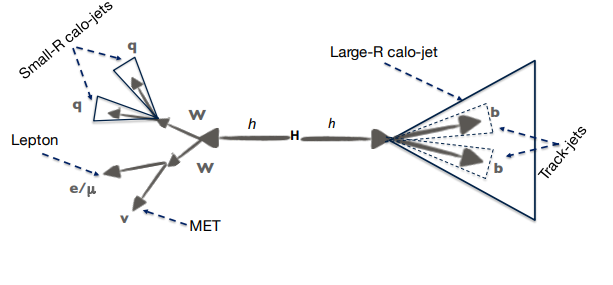
\includegraphics[width=0.9\textwidth]{figures/boosted_topo}
\caption{Diagram of the reconstructed event topology}
\label{fig:boost_topo}
\end{center}
\end{figure}

\subsection{Event Selection}
\label{sec:boosted_selection}
After the event is reconstructed, a b-jet veto is applied on the event by requiring all signal small-R jets do not pass b-tagging requirement to reject \ttbar events. The two highest \pT track-jets in the large-R jet are required to be b-tagged and events that passes this requirement is considered to be in the ``2-tag" region. In addition, the \met{} is required to be more than 50 GeV to reject events from QCD multijet background.%The cutflow for MC backgrounds and signal samples are documented in Appendix \ref{} and studies on the efficiency of the event reconstruction and selections can be found in Appendix \ref{}.

\subsection{Kinematic Selection}
\subsubsection{Signal Region}
\label{sec:boosted_regiondefs}
In order to enhance the sensitivity to a resonant HH signal, similarly to the resolved analysis, it is required
that the ${H\rightarrow b\overline{b}}$ candidate large-R jet has a mass consistent with the Standard Model Higgs boson mass.
Events which have the ${H\rightarrow b\overline{b}}$ candidate large-R jet mass in a window of ${90 \text{ GeV} < m_{\mathrm{Large-R jet}} < 140 \text{ GeV}}$ is considered to be in the signal region (SR).
The signal region is blinded and the blinding strategy is implemented by removing any events in data that passes the signal region requirement on the large-R jet mass.

\subsubsection{mBB Control Region}
In order to asses the modeling of the backgrounds, a control region is defined to be any events which fails the large-R jet signal region mass window requirement. Any event which has a large-R jet mass
 ${90 \text{ GeV} < m_{\mathrm{Large-R jet}}}$
 or ${m_{\mathrm{Large-R jet}} > 140 \text{ GeV}}$ 
 falls in the mBB control region (mBBcr). By construction, this region is orthogonal to the signal region.

\subsection{Multijet Background}
As with the resolved analysis, the QCD multijet background is estimated using the same data-driven method with slight modifications. 
 
The ABCD method uses three control regions (the B, C, and D regions) to estimate the contribution of a given background
in the signal (A) region.  Cuts on two ideally orthogonal variables are used to create the signal and various control regions,
e.g. the A region passes both cuts, the B and C regions each pass one cut and fail the other, while the D region fails both cuts.
 
For the boosted analysis, the ABCD regions are defined by using the same variables as in the resolved analysis, which are the significance of
the lepton impact parameter ($d_{0}^{\textrm{sig}}$) and the missing transverse momentum ($\met$). A small difference would be the higher cut value for the $\met$
with respect to the resolved analysis. The regions are defined as follow:
 
\begin{itemize}
\item Region A: \met $>$ 50 GeV, $|d_{0}^{\textrm{sig}}|$ $<$ 2.0
\item Region B: \met $<$ 50 GeV, $|d_{0}^{\textrm{sig}}|$ $<$ 2.0
\item Region C: \met $>$ 50 GeV, $|d_{0}^{\textrm{sig}}|$ $>$ 2.0
\item Region D: \met $<$ 50 GeV, $|d_{0}^{\textrm{sig}}|$ $>$ 2.0
\end{itemize}
 
\begin{figure}[!h]
\begin{center}
\includegraphics*[width=0.9\textwidth]{./figures/boosted/ABCD}
\caption[Regions defined in the ABCD method]{Regions defined in the ABCD method based on the lepton $d_{0}$ significance vs \met{} plane. Region A is the
signal enriched region which we want to estimate the multijet background. Region C is where the shape template is derived from and used
as shape prediction of the multijet background in region A. The ratio of the multijet yields in region B to region D is used to scale the multijet
yield in region C to predict the multijet background yield in region A.}
\label{fig:boosted_bkgd_abcd}
\end{center}
\end{figure}
 
Figure~\ref{fig:boosted_bkgd_abcd} shows the four regions represented on on the lepton $d_{0}$ significance vs \met{} plane.
Assuming that the two variables chosen to define the ABCD regions are completely uncorrelated, the QCD multijet yield in region A can be predicted. The The correlation between $|d_{0}^{\textrm{sig}}|$ vs \met{} is estimated in multiple MC background samples and also in data, and they are found to negligible.% (Appendix~\ref{app:boosted_qcd_d0met_plots}).
 
The ABCD method is done separately between the muon and electron channel as it is expected that the $\frac{N_B^\text{QCD}}{N_D^\text{QCD}}$ ratio and QCD multijet contribution to the total predicted background will be significantly different between the channels.
 
 %%%%%%%%%%%%%%%%%%%%%%%%%%%%%%%
%
% Yield prediction
%
%%%%%%%%%%%%%%%%%%%%%%%%%%%%%%%
\subsubsection{Yield prediction}
\label{sec:boosted_bkgd_qcdmultijet_yield}
 
Table~\ref{tab:boosted_region_bd_promptbkgd_data} lists the MC predicted prompt lepton backgrounds, observed data
and calculated multijet yields in Region B and D before the large-$R$ jet mass is applied and Table~\ref{tab:boosted_region_c_promptbkgd_data}
shows the yields in Region C mBB control region and signal region.
 
\begin{table}
\begin{center}
\begin{tabular}{l|c|c||c|c}
             &\multicolumn{2}{c||}{Region B}                &\multicolumn{2}{c}{Region D} \\
\hline
Samples       & Electron               & Muon                & Electron          & Muon \\      
\hline
$t\bar{t}$    &  307.7 $\pm$ 11.5      & 279.8 $\pm$ 10.6    & 21.3 $\pm$ 2.7    & 18.3  $\pm$ 2.6  \\
W+Jets        &  173.2 $\pm$ 5.2       & 179.3 $\pm$ 5.6     & 11.6 $\pm$ 1.4    & 10.6  $\pm$ 1.1  \\        
Single-top    &  42.9  $\pm$ 3.4       & 33.5  $\pm$ 3.6     &  3.0 $\pm$ 0.9    &  0.8  $\pm$ 0.5  \\
Z+Jets        &  78.5  $\pm$ 1.9       & 72.5  $\pm$ 1.7     &  6.4 $\pm$ 0.6    &  5.5  $\pm$ 0.5  \\
Dibosons      &  19.1  $\pm$ 1.5       & 17.7  $\pm$ 1.5     &  1.6 $\pm$ 0.4    &  2.2  $\pm$ 0.8  \\
\hline
Total Prompt  &  621.3 $\pm$ 13.2      & 582.7 $\pm$ 12.7    & 44.0 $\pm$ 3.3    & 37.4  $\pm$ 3.0  \\
\hline
Data          &  1003  $\pm$ 31.7      & 711   $\pm$ 26.7    & 144  $\pm$ 12.0   & 98    $\pm$ 9.9  \\
\hline
QCD           & 381.7 $\pm$ 34.3       & 128.3 $\pm$ 29.5    & 100.0 $\pm$ 12.4  & 60.6 $\pm$ 10.4 \\
\end{tabular}
\end{center}
\caption[MC predicted prompt lepton backgrounds, observed data and calculated multijet yields
in Region B and D]{MC predicted prompt lepton backgrounds, observed data and calculated multijet yields
in Region B and D. The multijet yield is calculated by subtracting the estimated total prompt lepton
backgrounds from the observed data. The statistical uncertainty on the yields is shown.}
\label{tab:boosted_region_bd_promptbkgd_data}
\end{table}
 
\begin{table}
\begin{center}
\begin{tabular}{l|c|c||c|c}
             &\multicolumn{2}{c||}{mBBcr}               &\multicolumn{2}{c}{SR}\\
\hline
Samples       & Electron            & Muon               & Electron         & Muon     \\      
\hline
$t\bar{t}$    &  38.7   $\pm$ 4.2   & 46.8  $\pm$ 7.9    & 28.5 $\pm$ 3.1   & 22.0 $\pm$ 2.7  \\
W+Jets        &  22.3   $\pm$ 2.0   & 20.0  $\pm$ 1.7    &  9.6 $\pm$ 1.3   & 10.0 $\pm$ 1.8  \\        
Single-top    &   7.6   $\pm$ 2.1   &  6.5  $\pm$ 1.3    &  7.1 $\pm$ 1.5   &  2.7 $\pm$ 0.8  \\
Z+Jets        &   4.6   $\pm$ 0.8   &  3.8  $\pm$ 0.5    &  1.6 $\pm$ 0.3   &  1.9 $\pm$ 0.6  \\
Dibosons      &   2.2   $\pm$ 0.6   &  1.2  $\pm$ 0.4    &  0.8 $\pm$ 0.3   &  1.7 $\pm$ 0.4  \\
\hline
Total Prompt  &  75.4   $\pm$ 5.2   & 78.4  $\pm$ 8.2    & 47.5 $\pm$ 3.7   & 38.3 $\pm$ 3.4  \\
\hline
Data          &  148    $\pm$ 12.2  & 126   $\pm$ 11.2   & 91   $\pm$ 9.5   & 71   $\pm$ 8.4  \\
\hline
QCD           & 72.6    $\pm$ 13.2  &  47.6 $\pm$ 13.9   & 43.5 $\pm$ 10.2  & 32.7 $\pm$ 9.1  \\
\end{tabular}
\end{center}
\caption[MC predicted prompt lepton backgrounds, observed data and calculated multijet yields
in Region C mBBcr and SR]{MC predicted prompt lepton backgrounds, observed data and calculated multijet yields
in Region C mBBcr and SR. The multijet yield is calculated by subtracting the estimated total prompt lepton
backgrounds from the observed data. The statistical uncertainty on the yields is shown.}
\label{tab:boosted_region_c_promptbkgd_data}
\end{table}
 
The $\frac{N_B^\text{QCD}}{N_D^\text{QCD}}$ ratio are calculated inclusively in the large-$R$ jet mass distribution.
In other words, the ratio is calculated without the jet mass window selection, which defines the SR and mBBcr, applied.
The ratio is then used to scale the QCD multijet yield in the SR and mBBcr of region C to predict the QCD multijet yield
in region A.
 
Table~\ref{tab:boosted_bkgd_abcd_ratio} shows the ratio in the electron channel and muon channel. As expected,
the electron channel ratio is larger than the muon channel. The muon channel ratio has a larger uncertainty due to
the more limited statistics in region B and region D compared to the electron channel. The predicted yields of the QCD multijet background
in the mBB control region and signal region are presented in Table~\ref{tab:boosted_bkgd_abcd_yield}. The QCD multijet background is
estimated to be ~19\% of the total background in the signal region (Table~\ref{tab:boosted_results_sr_yields}).
 
\begin{table}
\begin{center}
\begin{tabular}{c|c|c}
Multijet yield in region              & Electron                & Muon   \\      
\hline
$N_B^\text{QCD}$                      & 381.7 $\pm$ 34.3      & 128.3 $\pm$ 29.5 \\
$N_D^\text{QCD}$                      & 100.0 $\pm$ 12.4      & 60.6 $\pm$ 10.4  \\
\hline
$N_{B}^\text{QCD}$/$N_{D}^\text{QCD}$     & 3.8 $\pm$ 0.6 (15.3\%) & 2.1 $\pm$ 0.6 (28.7\%)   \\
\end{tabular}
\end{center}
\caption[Multijet yields in region B and region D and also the ratio of the yields for each lepton channel]{Multijet yields in region B and region D and also the ratio of the yields for each lepton channel. The error
on the $\frac{N_B^\text{QCD}}{N_D^\text{QCD}}$ ratio is propagated from the statistical uncertainties on the multijet yields in each region.}
\label{tab:boosted_bkgd_abcd_ratio}
\end{table}
 
\begin{table}[!htbp]
\begin{center}
\begin{tabular}{c|c|c}
Multijet yield in region & Electron  & Muon  \\  
\hline
\multicolumn{3}{c}{SR} \\
\hline
$N_C^\text{QCD}$         & 43.4  $\pm$ 10.2 & 32.7 $\pm$ 9.1 \\
$N_A^\text{QCD}$         & 165.9 $\pm$ 46.6 (28.1\%) & 69.3 $\pm$ 27.7 (39.9\%) \\
\hline
\multicolumn{3}{c}{mBBcr} \\
\hline
$N_C^\text{QCD}$       & 72.6  $\pm$ 13.2 & 47.6  $\pm$ 13.9  \\
$N_A^\text{QCD}$       & 277.1 $\pm$ 66.0 (23.8\%) & 100.8 $\pm$ 41.3 (41.0\%)  \\
\hline
\end{tabular}
\end{center}
\caption[Multijet yield in region C and predicted yield in region A in the SR]{Multijet yield in region C and predicted yield in region A in the SR. The error on $N_A^\text{QCD}$
are propagated from the error on the $N_B^\text{QCD}$/$N_D^\text{QCD}$ ratio and statistical uncertainty on $N_C^\text{QCD}$ yield.
The numbers in brackets are the relative uncertainty in percentage.}
\label{tab:boosted_bkgd_abcd_yield}
\end{table}
 
\FloatBarrier
 
%%%%%%%%%%%%%%%%%%%%%%%%%%%%%%%
%
% Shape prediction
%
%%%%%%%%%%%%%%%%%%%%%%%%%%%%%%%
\subsubsection{Shape prediction}
\label{sec:boosted_bkgd_qcdmultijet_shape}
In order to predict the shape of the HH mass distribution (and also other kinematic distribution) of the QCD multijet background, the shape template of all kinematic distributions are obtained by subtracting all the MC backgrounds from data
in region C.
 
It was found that distributions in region C suffer from lack of statistics due the low number of data events which results in shape templates with severe statistical fluctuations. To overcome this, the shape templates are derived from a sample of 1 $b$-tagged (1-tag) events in region C. This sample requires that one of the two leading track-jet is $b$-tagged but not both at the same time.% Comparisons between 2-tag and 1-tag shape templates are documented in Appendix~\ref{app:boosted_qcd_2tag1tag}.
 
%%%%%%%%%%%%%%%%%%%%%%%%%%%%%%%
%
% Normalization Uncertainties
%
%%%%%%%%%%%%%%%%%%%%%%%%%%%%%%%
\subsubsection{Multijet yield uncertainties}
\label{sec:boosted_bkgd_qcdmultijet_yield_unc}
 
%%%%%%%%%%%%%%%%%%%%%%%%%%%%%%%
% Statistical
%%%%%%%%%%%%%%%%%%%%%%%%%%%%%%%
\paragraph{Statistical} 
The uncertainty on the predicted yield of the multijet background is determined by propagating the statistical uncertainty
of the $\frac{N_B^\text{QCD}}{N_D^\text{QCD}}$ ratio, as shown in Table~\ref{tab:boosted_bkgd_abcd_ratio}, and the statisical
uncertainty on the multijet yield in region C ($N_C^\text{QCD}$), as in Table~\ref{tab:boosted_bkgd_abcd_yield}.
 
\paragraph{1-tag/2-tag jet mass acceptance} 
Another source of uncertainty on the multijet yield is the  
the difference of acceptance of the large-$R$ jet mass cut between 1-tag and 2-tag.
This uncertainty is included since the template for or the multijet shape prediction uses the multijet shape
from the 1-tag region C. Table~\ref{tab:boosted_syst_qcd_norm_mBBAcc} shows the acceptance
of the large-$R$ jet mass signal and mBB control region selection in the multijet 1-tag region C and 2-tag region C yields.
The relative difference between the acceptance in 1-tag region C and in 2-tag region C is considered as an uncertainty on the normalization
of the QCD multijet prediction.
 
\begin{table}[!htbp]
\begin{center}
\begin{tabular}{c|c|c}
\hline
Region    & Electron          & Muon      \\
\hline
\multicolumn{3}{c}{SR} \\
\hline
1-tag $\frac{N_\text{SR}}{N_\text{Inc}}$ &  31.6 $\pm$ 2.7 \% & 27.9 $\pm$ 2.7 \% \\
2-tag $\frac{N_\text{SR}}{N_\text{Inc}}$ &  37.5 $\pm$ 9.7 \% & 40.7 $\pm$ 9.7 \% \\
\hline \hline
Rel. difference between 1-tag and 2-tag & 15.6 \% & 31.5 \% \\
\hline
\multicolumn{3}{c}{mBBcr} \\
\hline
1-tag $\frac{N_\text{mBBcr}}{N_\text{Inc}}$ &  68.4 $\pm$ 2.7  \% & 72.1 $\pm$ 2.7 \% \\
2-tag $\frac{N_\text{mBBcr}}{N_\text{Inc}}$ &  62.5 $\pm$ 7.0  \% & 59.3 $\pm$ 7.0 \% \\
\hline \hline
Rel. difference between 1-tag and 2-tag &  9.4 \% &   21.6 \% \\
\end{tabular}
\end{center}
\caption[The acceptance of the large-$R$ jet mass signal region selection on the multijet
1-tag and 2-tag region C]{The acceptance of the large-$R$ jet mass signal region selection on the multijet
1-tag and 2-tag region C. $N_\text{SR}$($N_\text{Inc}$) is the multijet yield
with (without) the signal region large-$R$ jet mass selection.}
\label{tab:boosted_syst_qcd_norm_mBBAcc}
\end{table}
 
%%%%%%%%%%%%%%%%%%%%%%%%%%%%%%%
% mBB control region fit
%%%%%%%%%%%%%%%%%%%%%%%%%%%%%%%
\paragraph{mBB control region fit} 
 A likelihood fit of the large-$R$ jet mass in the mBB control region
is performed with the normalization of the multijet background to be unconstrained in the fit.
%This study is documented in Appendix~\ref{app:boosted_qcd_float_2tag_mbbcr_fit}. 
In the muon channel,
the post-fit normalization factor is consistent with unity and in the electron channel,
the normalization factor is 0.676 $\pm$ 0.130. Due to this significant deviation from unity for the electron channel,
we assign a normalization uncertainty of 32.4\% for the multijet background in both the mBB control
region and signal region.
 
%%%%%%%%%%%%%%%%%%%%%%%%%%%%%%%
% ttbar and W+jets MC modeling
%%%%%%%%%%%%%%%%%%%%%%%%%%%%%%%
\paragraph{$t\bar{t}$ and W+jets MC modeling}
 The uncertainties on the MC modeling
of the $t\bar{t}$ and W+jets, the two largest prompt background predicted by MC in region B,D and C
are taken as a systematic on the predicted multijet background in region A since the multijet
background is calculated by subtracting the prompt background from observed data. The uncertainties
on the normalization of $t\bar{t}$ and W+jets in each region are calculated by comparing the yields
between the nominal $t\bar{t}$ and W+jets samples with their alternative samples
(see Section~\ref{sec:boosted_syst_modeling_top} and~\ref{sec:boosted_syst_modeling_vjets}).
%The comparisons are documented in Appendix~\ref{app:boosted_qcd_region_mcmodeling_unc}.
 
The uncertainty on the multijet yield prediction in region A is then calculated
by recalculating the multijet yield in each region with the $t\bar{t}$ and W+jets
yields be varied up and down, simultaneously in all regions, by the uncertainty due to the
MC modeling of the background. The resulting multijet yield prediction in region A for
each background uncertainty is then compared to the nominal prediction in region A and the difference is
then taken as the uncertaintyon the multijet yield prediction in region A.
Table~\ref{tab:boosted_syst_qcd_norm_ttbarwjetsregionc} shows the uncertainty on the multijet yield prediction
in region A signal and mBB control region  due to the the uncertainty on the $t\bar{t}$ and W+jets
MC modeling.
 
\begin{table}[!htbp]
\begin{center}
\begin{tabular}{c|c|c}
& Electron  & Muon  \\  
\hline
\multicolumn{3}{c}{SR} \\
\hline
$t\bar{t}$           &     26.5 \% &   60.1 \%  \\
W+jets               &     24.7 \% &   70.4 \%  \\
\hline
\multicolumn{3}{c}{mBBcr} \\
\hline
$t\bar{t}$           &  37.4  \%  &   101.0\%  \\
W+jets               &  29.5  \%  &   77.6\%   \\
\hline
\end{tabular}
\end{center}
\caption[The uncertainty on the multijet yield prediction in region A]{The uncertainty on the multijet yield prediction in region A due to the normalization
uncertainty of the $t\bar{t}$ and W+jets backgrounds in region C.}
\label{tab:boosted_syst_qcd_norm_ttbarwjetsregionc}
\end{table}
 
%%%%%%%%%%%%%%%%%%%%%%%%%%%%%%%
% Detector modeling
%%%%%%%%%%%%%%%%%%%%%%%%%%%%%%%
\paragraph{Detector modeling of prompt backgrounds}
 The detector modeling systematic uncertainties
on the prompt background in regions B, D and C are propagated through the ABCD method to estimate
the uncertainty on the multijet yield prediction region A. Table~\ref{tab:boosted_syst_qcd_norm_detmodel}
shows the uncertainties on the predicted multijet yield in both lepton channels. %The impact of each detector modeling systematics on the predicted multijet yield are listed in Appendix~\ref{app:boosted_qcd_prompt_detector_modeling_unc}.
 
\begin{table}[!htbp]
\begin{center}
\begin{tabular}{c|c|c}
& Electron  & Muon  \\  
\hline
\multicolumn{3}{c}{SR} \\
\hline
Total Uncertainty          &  46.0\%  &  105.6\%   \\
\hline
\multicolumn{3}{c}{mBBcr} \\
\hline
Total Uncertainty          &  45.5\%  &  127.3  \%   \\
\hline
\end{tabular}
\end{center}
\caption{The total uncertainty on the multijet yield prediction in region A due to the detector modeling
uncertainties of the prompt backgrounds in region B, C and D.}
\label{tab:boosted_syst_qcd_norm_detmodel}
\end{table}
 
%%%%%%%%%%%%%%%%%%%%%%%%%%%%%%%
% d0sig cut efficiency
%%%%%%%%%%%%%%%%%%%%%%%%%%%%%%%
\paragraph{$\mathbf{|d_{0}^{\textrm{sig}}|}$ cut efficiency modeling}
The $|d_{0}^{\textrm{sig}}|$ cut efficiency modeling uncertainty for the prompt MC backgrounds
are also taken into account in the ABCD method due to the tigther cut on the leptons' $|d_{0}^{\textrm{sig}}|$,
than the recommended value. The determination of the $|d_{0}^{\textrm{sig}}|$ cut efficiency modeling uncertainty
is discussed in Section~\ref{sec:boosted_syst_d0cut}. This uncertainty is propagated through the ABCD method
by varying the normalization of the prompt backgrounds in regions B, D and C simultaneously to estimate
the uncertainty on the multijet yield prediction region A and is treated as anti-correlated between regions B and regions D,C.
Table~\ref{tab:boosted_syst_qcd_norm_d0sigacc} shows the uncertainties on the predicted multijet yield due
$|d_{0}^{\textrm{sig}}|$ cut efficiency modeling uncertainty on prompt MC backgrounds in both lepton channels.
%The breakdown of the multijet yield and its variation due to the $|d_{0}^{\textrm{sig}}|$ cut efficiency modeling uncertainty on the prompt MC backgrounds in each region and channel is listed in Table~\ref{tab:boosted_qcd_d0syst_breakdown} of Appendix~\ref{app:boosted_qcd_prompt_d0cut_modeling_unc}.
 
\begin{table}[!htbp]
\begin{center}
\begin{tabular}{c|c|c}
& Electron  & Muon  \\  
\hline
\multicolumn{3}{c}{SR} \\
\hline
Total Uncertainty          &  46.4\%  &  50.9\%   \\
\hline
\multicolumn{3}{c}{mBBcr} \\
\hline
Total Uncertainty          &  42.0\%  &  110.6\%   \\
\hline
\end{tabular}
\end{center}
\caption{The total uncertainty on the multijet yield prediction in region A due to the $|d_{0}^{\textrm{sig}}|$
cut efficiency modeling uncertainties of the prompt backgrounds in region B, D and C.}
\label{tab:boosted_syst_qcd_norm_d0sigacc}
\end{table}
 
%%%%%%%%%%%%%%%%%%%%%%%%%%%%%%%
% Total uncertainty
%%%%%%%%%%%%%%%%%%%%%%%%%%%%%%%
\paragraph{Total uncertainty on the yield}
 The total uncertainty on the multijet prediction
is calculated as the sum in quadrature of the uncertainties from the two sources explained above.
Table~\ref{tab:boosted_syst_qcd_norm_unc_final} summarizes the systematic uncertainties on the predicted
multijet yield in the electron channel and the muon channel.
 
\begin{table}[!htbp]
\begin{center}
\begin{tabular}{c|c|c}
Source of uncertainty &  Electron  & Muon  \\  
\hline
\multicolumn{3}{c}{SR} \\
\hline
Statistical                                      &  28.1 \% & 39.9 \% \\
2-tag/1-tag jet mass acceptance                  &  15.6 \% & 31.5 \% \\
mBB control region fit                           &  32.3 \% & - \\
$t\bar{t}$ MC modeling                          &  26.5 \% & 60.1\% \\
W+jets modeling                                 &  24.7 \% & 70.4\% \\
Detector modeling of prompt backgrounds         &  46.0 \% & 105.6\% \\
$|d_{0}^{\textrm{sig}}|$ cut efficiency          &  46.4 \% & 50.9\% \\
\hline
Total                                            &  87.5 \% & 157.8 \% \\
\hline
\hline
\multicolumn{3}{c}{mBBcr} \\
\hline
Statistical                                      &  23.8 \% & 41.0 \% \\
2-tag/1-tag jet mass acceptance                  &  9.4  \% & 21.6 \% \\
mBB control region fit                           &  32.3 \% & -       \\
$t\bar{t}$ MC modeling                          &  37.4 \% & 101.0\% \\
W+jets MC modeling                              &  29.5 \% & 77.6\% \\
Detector modeling of prompt backgrounds         &  45.5 \% & 127.3\% \\
$|d_{0}^{\textrm{sig}}|$ cut efficiency          &  42.0 \% & 110.6\% \\
\hline
Total                                            &  88.3 \% & 216.4 \% \\
\end{tabular}
\end{center}
\caption[Summary of systematic uncertainties on the QCD multijet yield in the signal region and mBB control region
for each lepton channel]{Summary of systematic uncertainties on the QCD multijet yield in the signal region and mBB control region
for each lepton channel. The total uncertainty calculated by adding in quadrature the uncertainties from all sources.}
\label{tab:boosted_syst_qcd_norm_unc_final}
\end{table}
 
%%%%%%%%%%%%%%%%%%%%%%%%%%%%%%%
%
% Shape Uncertainties
%
%%%%%%%%%%%%%%%%%%%%%%%%%%%%%%%
\subsubsection{Multijet shape uncertainties}
\label{sec:boosted_bkgd_qcdmultijet_shape_unc}
 
The uncertainty on the $m_{HH}$ distribution prediction for the QCD multijet background is estimated by comparing
the $m_{HH}$ distribution shape in the 2-tag region C and 1-tag region C (Figure~\ref{fig:boosted_abcd_shapesyst}).
 
\begin{figure}[!h]
\begin{center}
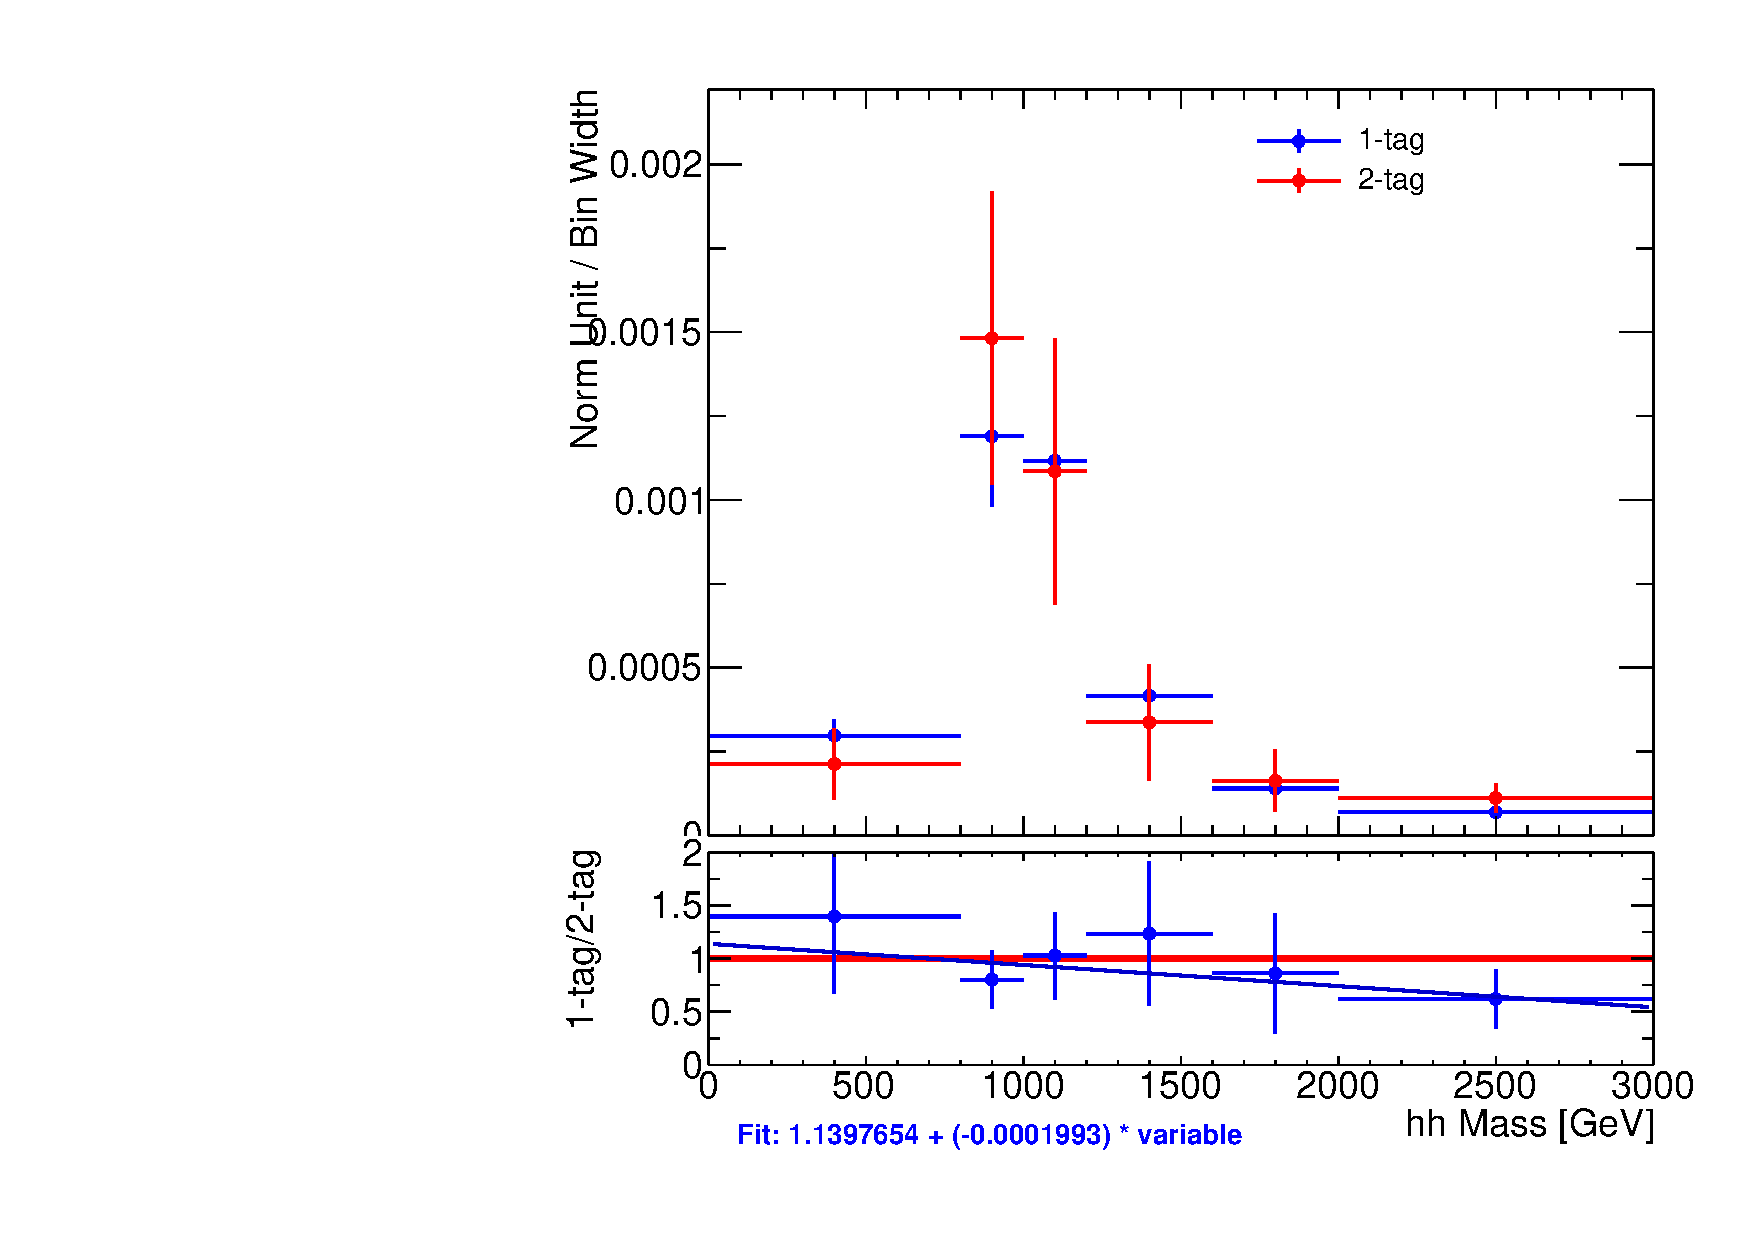
\includegraphics[width=0.49\textwidth]{./figures/boosted/ABCD/QCD_SR_hhMass.pdf}
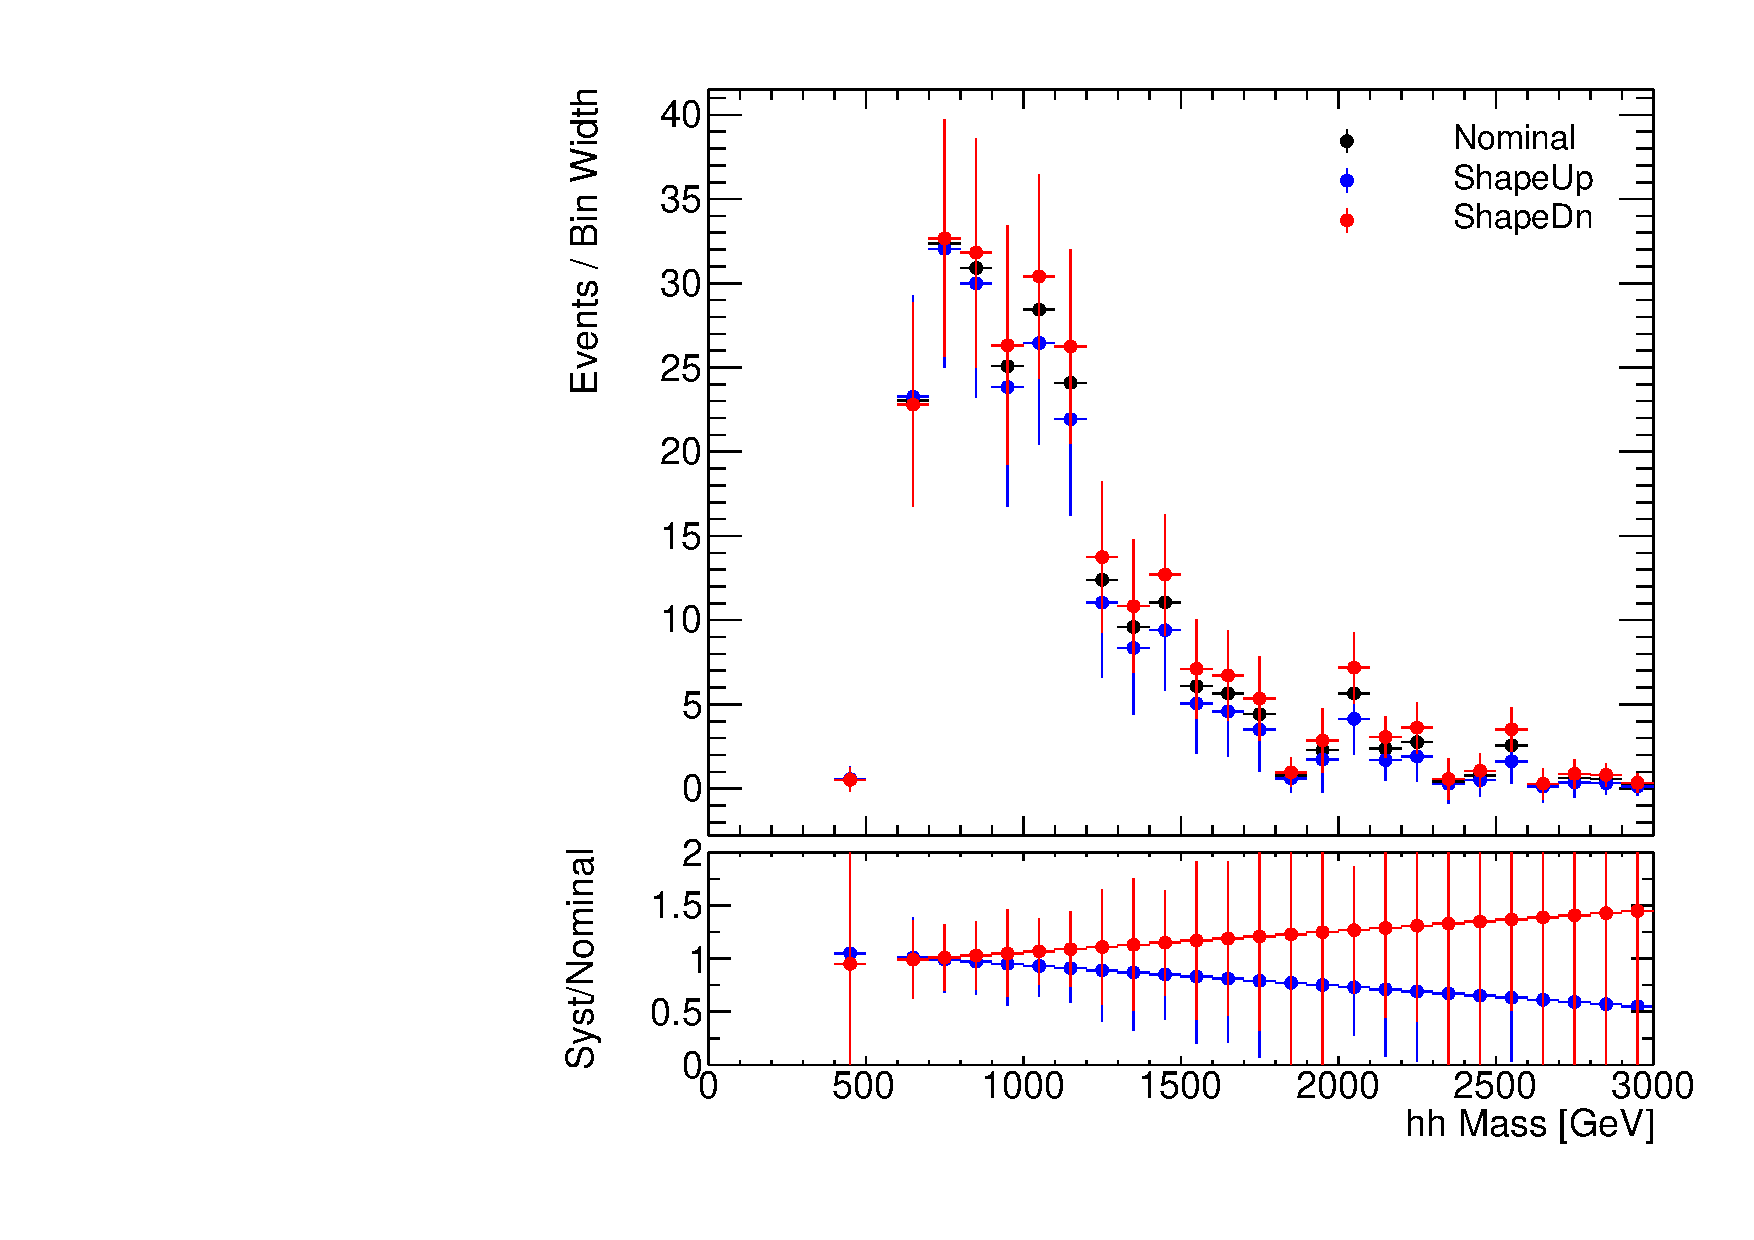
\includegraphics[width=0.49\textwidth]{./figures/boosted/ABCD/Fit_QCD_SR_hhMass.pdf}
\caption[Shape comparison of the $m_{HH}$ distribution in region C of the 1-tag and 2-tag region]{(a) Shape comparison of the $m_{HH}$ distribution in region C of the 1-tag and 2-tag region.
The linear fit to the ratio is used as the shape systematic of QCD background prediction.
(b) The up and down QCD shape systematic variation for the predicted $m_{HH}$ distribution.}
\label{fig:boosted_abcd_shapesyst}
\end{center}
\end{figure}

%%%%%%%%%%%%%%%%%%%%%%%%%%%%%%%
%
% Final prediction
%
%%%%%%%%%%%%%%%%%%%%%%%%%%%%%%%
\subsubsection{Final prediction and validation}
\label{sec:boosted_bkgd_qcdmultijet_predict_valid}
 
The predicted multijet yield and its uncertainty in the signal region and mBB control region are
shown in Table~\ref{tab:boosted_syst_qcd_norm_unc}.
 
\begin{table}[!htbp]
\begin{center}
\begin{tabular}{l|c|c|c}
Region    & Electron                   & Muon                       & Combined                   \\  
\hline
SR        & 165.9 $\pm$ 145.2(87.5\%) & 69.3 $\pm$ 109.3(157.8\%)   & 235.2 $\pm$ 181.8 (77.3\%) \\
mBBcr     & 277.1 $\pm$ 244.8(88.3\%) & 100.8 $\pm$ 218.1(216.4\%)  & 377.9 $\pm$ 327.8 (86.8\%) \\
\hline
\end{tabular}
\end{center}
\caption[Predicted multijet yield in the SR and mBBcr]{Predicted multijet yield with uncertainties in the signal region (SR) and mBB control region (mBBcr)
for each lepton channel.}
\label{tab:boosted_syst_qcd_norm_unc}
\end{table}
 
The ABCD method is validated by assessing the agreement of data and total background prediction with the QCD multijet background included
in the mBB control region. This is discussed in Section~\ref{sec:boosted_bkgd_datavspred}.
 
%
% ttbar
%
\subsection{$\mathbf{t\bar{t}}$}
\label{sec:boosted_bkgd_ttbar}
 
MC simulation is used to model the shape of the $t\bar{t}$ background. The background
is predicted to be the largest ($\sim$ 52\%) of the total background. A top-enriched control region
is used to validate the modeling of the $t\bar{t}$ background.% and the comparison between Data andbackground prediction is documented in Appendix~\ref{app:boosted_ttbarmodel_topcr}.
% The normalization of the $t\bar{t}$ background is obtained by fitting the large-$R$ jet mass distribution
% in the mBB control region and extract the normalization factor on the $t\bar{t}$ normalization from the fit.
% Both the $t\bar{t}$ and W+jets backgrounds are allowed to float simultaneously in the fit. The studies are documented in
% Appendix ~\ref{app:boosted_fitstudies_mBBcr}.
 
%
% V+jets
%
\subsection{V+jets}
\label{sec:boosted_bkgd_vjets}
 
MC simulation is used to model the shape and predict the yield of the W+jets and Z+jets background.
The W+jets background is predicted to be the third largest background ($\sim$ 18\%) of the total background while
the Z+jets background is expected to be $\sim$ 2\% in the signal region (Table~\ref{tab:boosted_results_sr_yields}).
 
%
% Single-top
%
\subsection{Single Top}
\label{sec:boosted_bkgd_singletop}
 
MC simulation is used to model the shape and predict the yield of background from single-top processes. This background is
predicted to be $\sim$ 9\% of the total background (Table~\ref{tab:boosted_results_sr_yields}).
The single-top background is predominantly consist of Wt production process
($\sim$ 90\%), followed by the t-channel production ($\sim$ 9\%) and the s-channel production ($\sim$ 1\%).
 
%
% Diboson
%
\subsection{Diboson}
\label{sec:boosted_bkgd_diboson}
MC simulation is used to model the shape and predict the yield of the diboson background. This background is predicted to be
~2\% of the total background in the signal region  (Table~\ref{tab:boosted_results_sr_yields}).
 
 
\subsection{Data/Prediction comparisons in control regions}
\label{sec:boosted_bkgd_datavspred}
 
To asses the modeling of the background, the total predicted background is asses with data in the mBB control region.
The electron channel and the muon channel are combined into a single channel.
 
Table~\ref{tab:boosted_bkgd_mbbcr_yields} shows the predicted yield of each background. The data, collected in 2015+2016,
corresponding to the integrated luminosity of 36.1 fb$^{-1}$ are used. The MC backgrounds $t\bar{t}$, W+jets,
Single-top, Z+jets and Dibosons are normalized to luminosity. The QCD multijet prediction is estimated from the ABCD method.
Statistical errors are shown for the individual backgrounds and the total predicted background while the error due
to systematic uncertainties are shown only for the total predicted background. Detector modeling uncertainties, MC background modeling
uncertainties and uncertainties from the ABCD method for QCD multijet background are considered.
The predicted total background yield has an error of about 27\% due to systematic uncertainties and
the observed yield in data is in good agreement with the total background yield.
 
Figure~\ref{fig:boosted_mbbcr_mainplots}, \ref{fig:boosted_mbbcr_largerjet}, \ref{fig:boosted_mbbcr_wwsystem},
\ref{fig:boosted_mbbcr_whad}, \ref{fig:boosted_mbbcr_wlep}, \ref{fig:boosted_mbbcr_lepton}, \ref{fig:boosted_mbbcr_whad_jets}
and \ref{fig:boosted_mbbcr_dr} show the distributions of kinematic variables for events which fall into the mBB control regions.
The observed data (black circle) corresponds to an integrated luminosity of 36.1 fb$^{-1}$. The MC backgrounds $t\bar{t}$ (orange), W+jets (blue),
Single-top (red), Z+jets (green) and Dibosons (yellow) are normalized to cross-section prediction scaled to luminosity of 36.1 fb$^{-1}$.
The QCD multijet background (grey) is predicted from the ABCD method. The hashed grey band is the statistical uncertainty on
the predicted background and the red box band is the statistical+systematics uncertainty on the predicted background.
The systematics uncertainty on the predicted background consists of the detector modeling systematic uncertainties,
MC background modeling uncertainties and uncertainties from the ABCD method for QCD multijet background.
 
Figure~\ref{fig:boosted_mbbcr_mainplots} is the invariant mass of the reconstructed di-Higgs (HH)system distribution, the $\met$, and $W \to l\nu$ system transverse mass distributions and as it can be seen that it is reasonably modelled. The good modeling observed of the
distributions gives confidence to the QCD multijet prediction as the events from the background tend to have
low values of $\met$ and transverse mass.
 
%In Appendix~\ref{app:boosted_mbbcontrolregion}, the kinematic distributions are shown separately in the low mBB and high mBB region of the mBB control region (App.~\ref{app:boosted_mbbcontrolregion_highlow}). The distributions separated by the lepton channels are also shown (App.~\ref{app:boosted_mbbcontrolregion_leptonchannels}).
 
\renewcommand{\arraystretch}{1.5}
\begin{table}
\begin{center}
\begin{tabular}{l|c|c|c}
Sample        &  Yield   &  Stats Unc &   Systs Unc \\
\hline
$t\bar{t}$    &  1005.6  & $\pm$ 20.6    &   $^{+283.6(+28.2\%)}_{-288.8(-28.7\%)}$ \\
W+Jets        &  565.6   & $\pm$ 10.3    &   $^{+277.9(+49.1\%)}_{-270.0(-47.7\%)}$ \\
QCD           &  377.9   & $\pm$ 19.6    &   $^{+328.0(+86.8\%)}_{-328.0(-86.8\%)}$ \\
Single-top    &  161.3   & $\pm$ 7.2     &   $^{+114.4(+70.9\%)}_{-114.4(-70.9\%)}$ \\
Z+Jets        &  55.9    & $\pm$ 1.6     &   $^{+27.7(+49.5\%)}_{-27.2(-48.6\%)}$ \\
Dibosons      &  39.7    & $\pm$ 2.6     &   $^{+23.4(+58.9\%)}_{-23.3(-58.7\%)}$ \\
\hline
Prediction    &  2206.0  & $\pm$ 31.2    &   $^{+593.7(+26.9\%)}_{-586.1(-26.6\%)}$ \\
Data          &  2179    & - & - \\
\hline
Data/Pred     &  0.99    & - & - \\
\hline
\end{tabular}
\end{center}
\caption[Predicted and observed yields in the mBB control region]{Predicted and observed yields in the mBB control region. Detector modeling
uncertainties, MC background modeling uncertainties and QCD background modeling uncertainties
from ABCD method are considered for the systematic uncertainties.}
\label{tab:boosted_bkgd_mbbcr_yields}
\end{table}
\renewcommand{\arraystretch}{1.0}
\newpage
\begin{figure}[!h]
\begin{center}
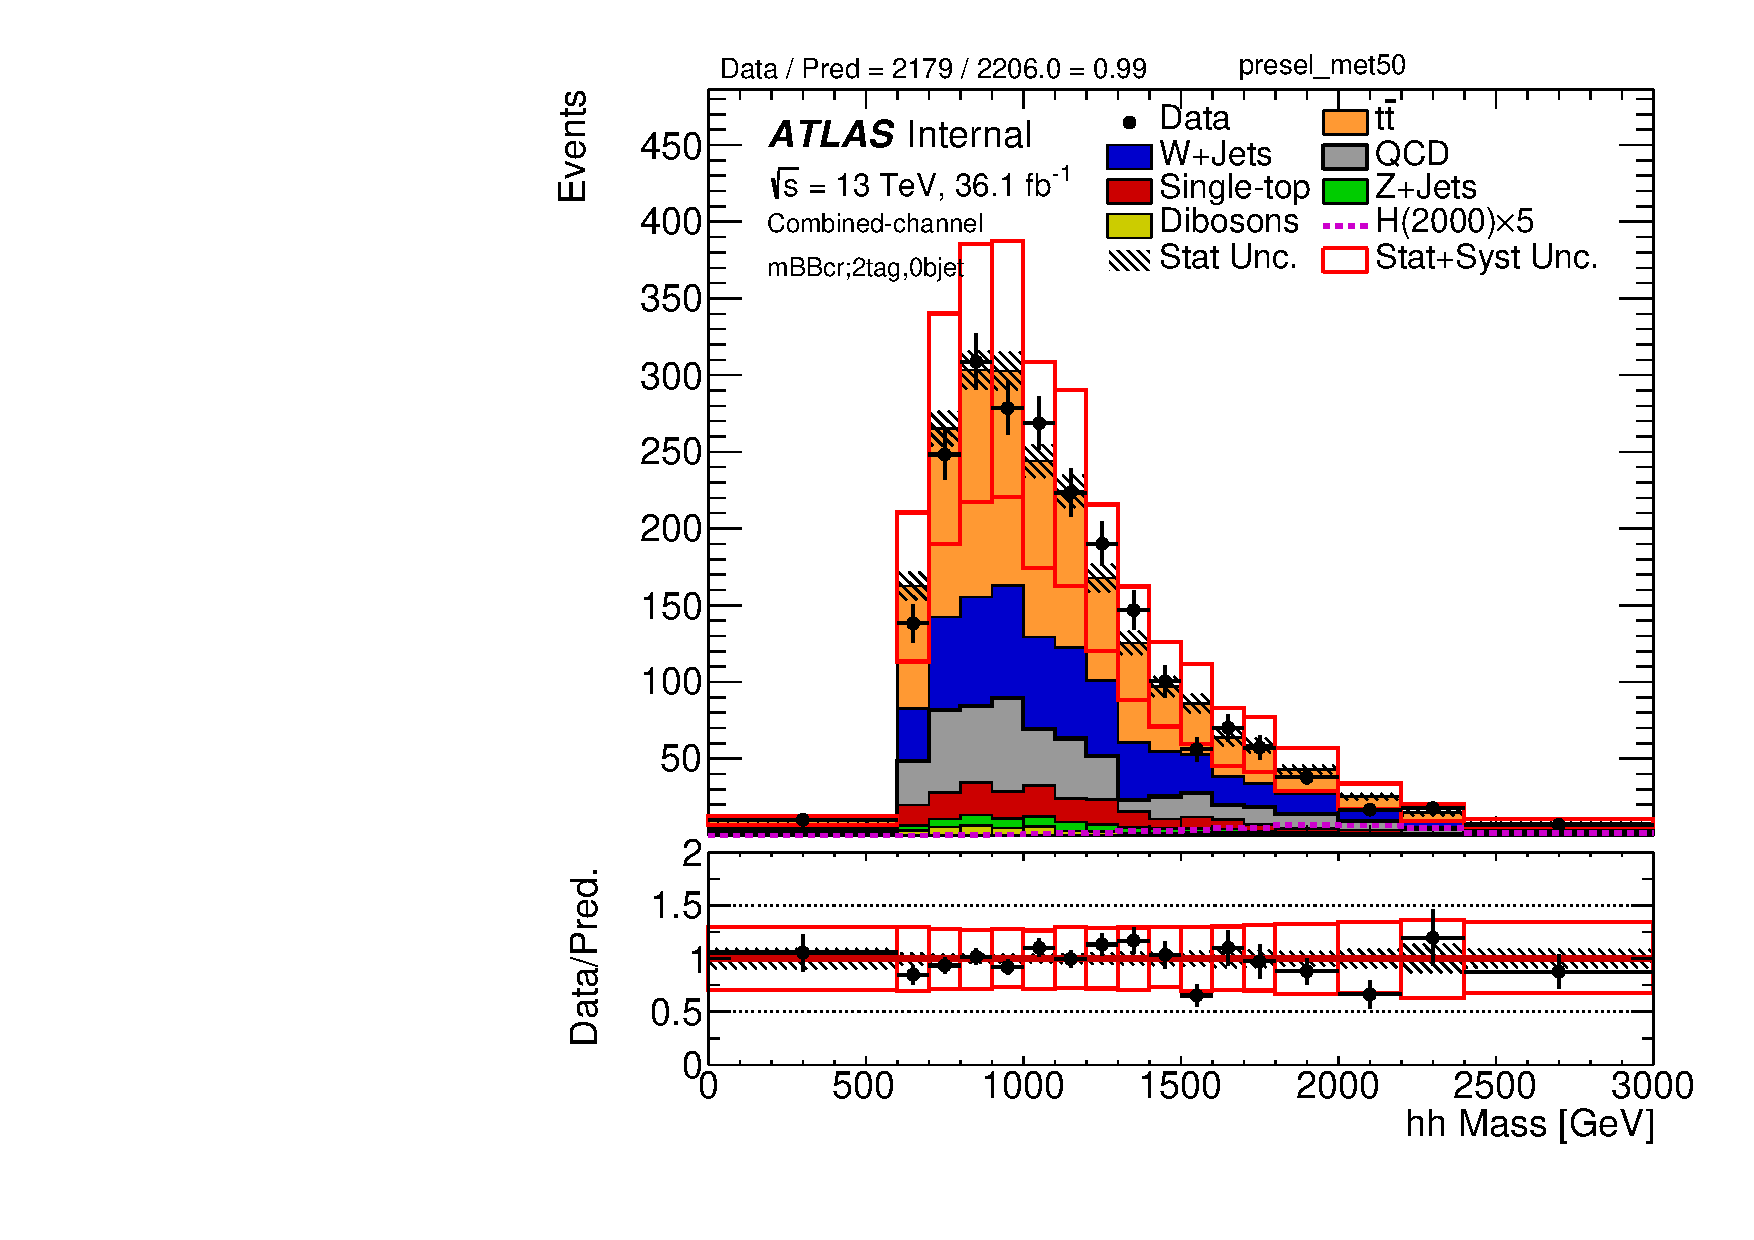
\includegraphics[width=0.49\textwidth]{./figures/boosted/PlotsInMbbCR/DataMC_2tag_0bjet_mbbcr_lepton_presel_met50_hhMassRebin1}
\par\medskip
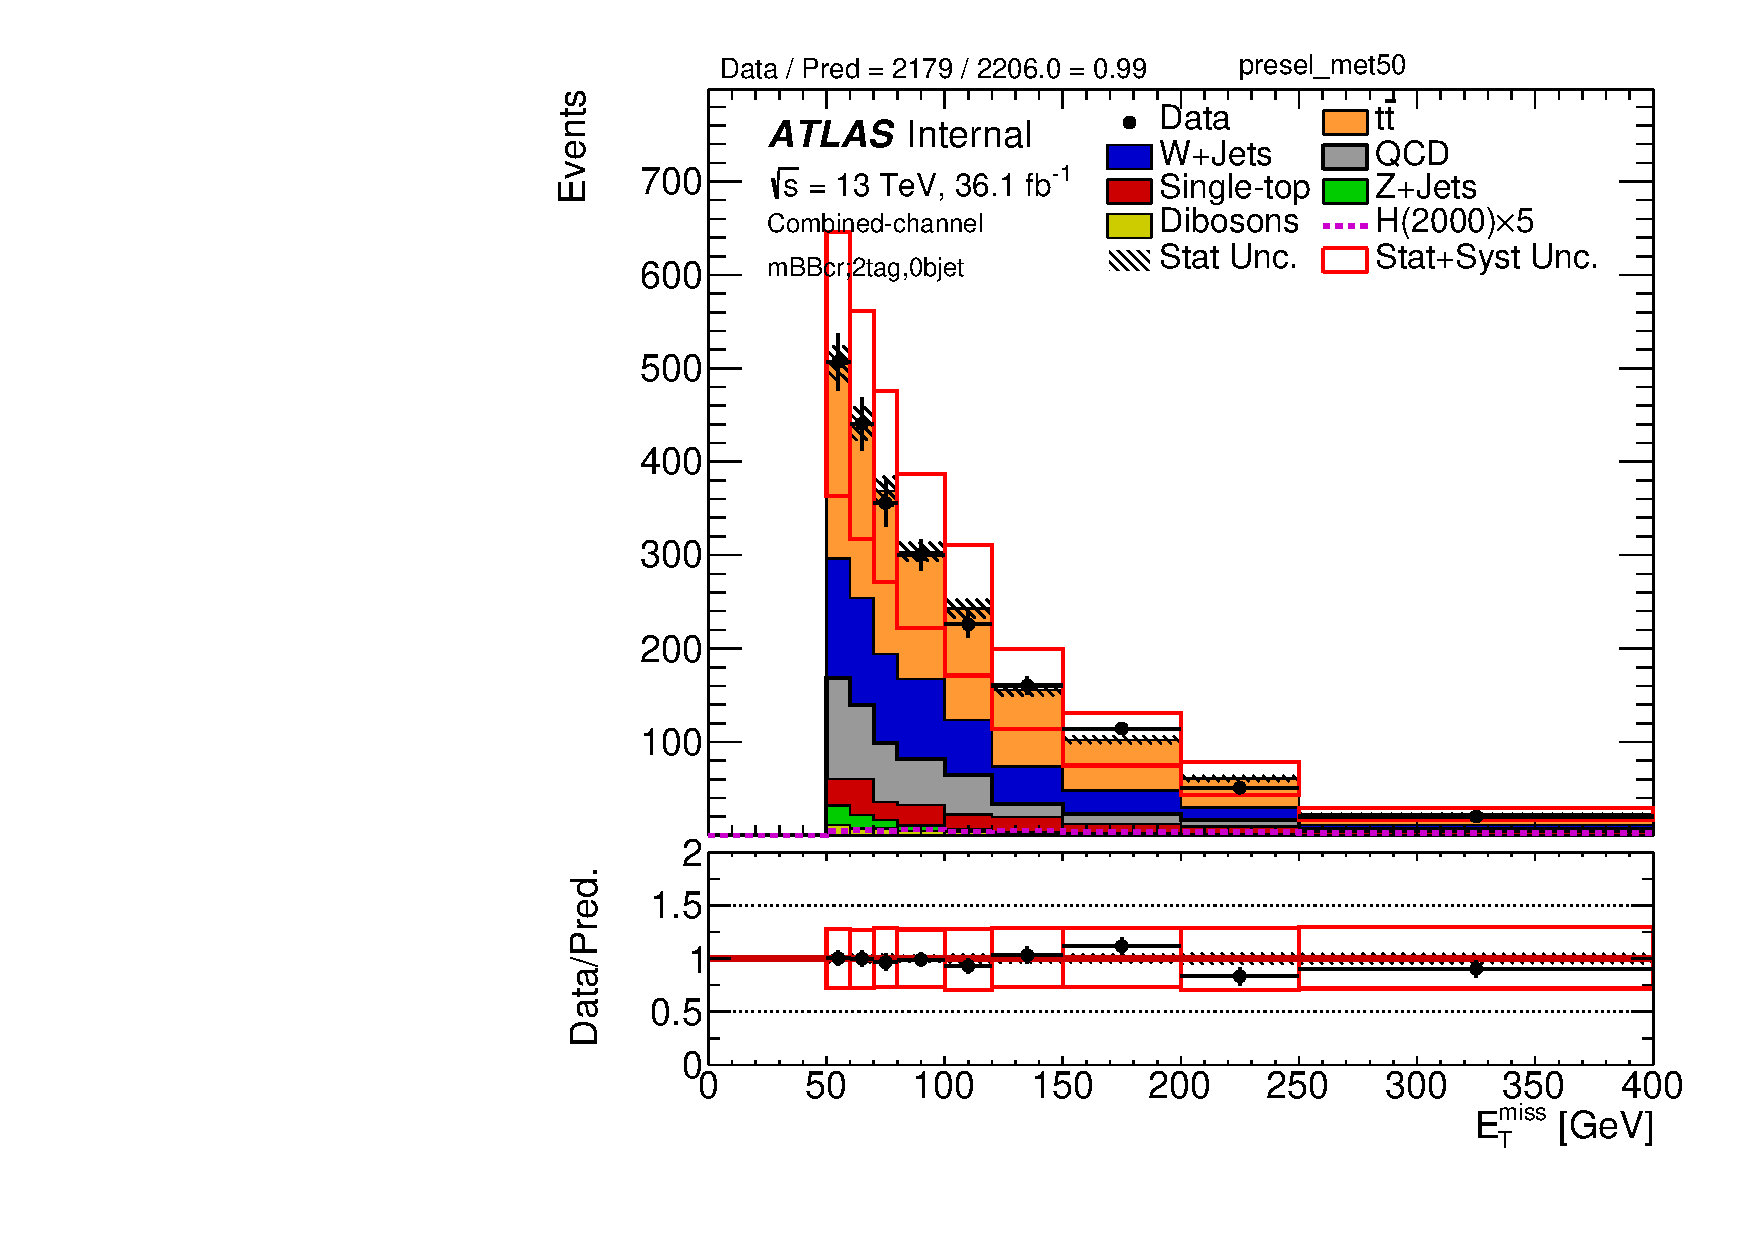
\includegraphics[width=0.49\textwidth]{./figures/boosted/PlotsInMbbCR/DataMC_2tag_0bjet_mbbcr_lepton_presel_met50_MET}
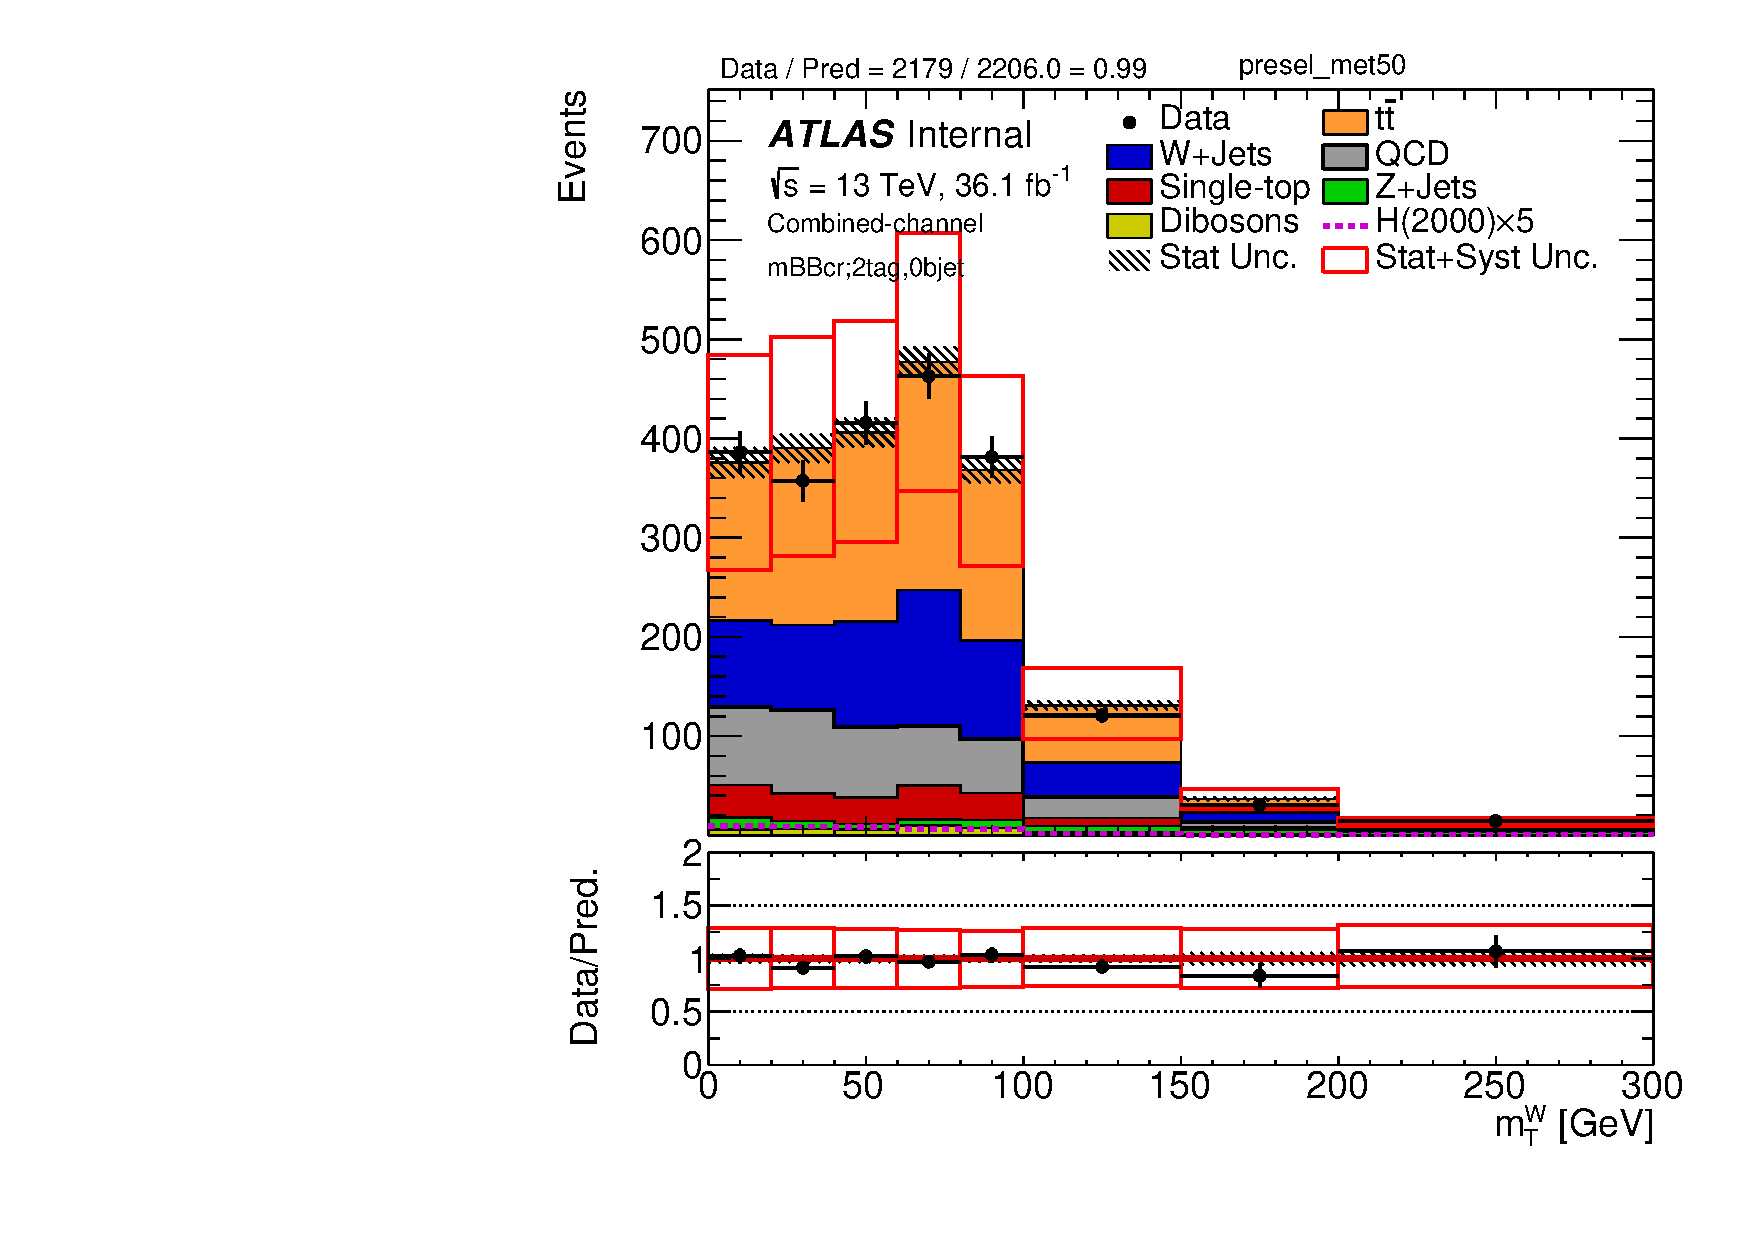
\includegraphics[width=0.49\textwidth]{./figures/boosted/PlotsInMbbCR/DataMC_2tag_0bjet_mbbcr_lepton_presel_met50_WlepMtATLAS}
\caption{The invariant mass of the reconstructed di-Higgs (HH) system, \met and transverse mass of the $W \to l\nu$ system
distributions of events in the mBB control region (mBBcr).}
\label{fig:boosted_mbbcr_mainplots}
\end{center}
\end{figure}
\newpage
% 
\begin{figure}[!h]
\begin{center}
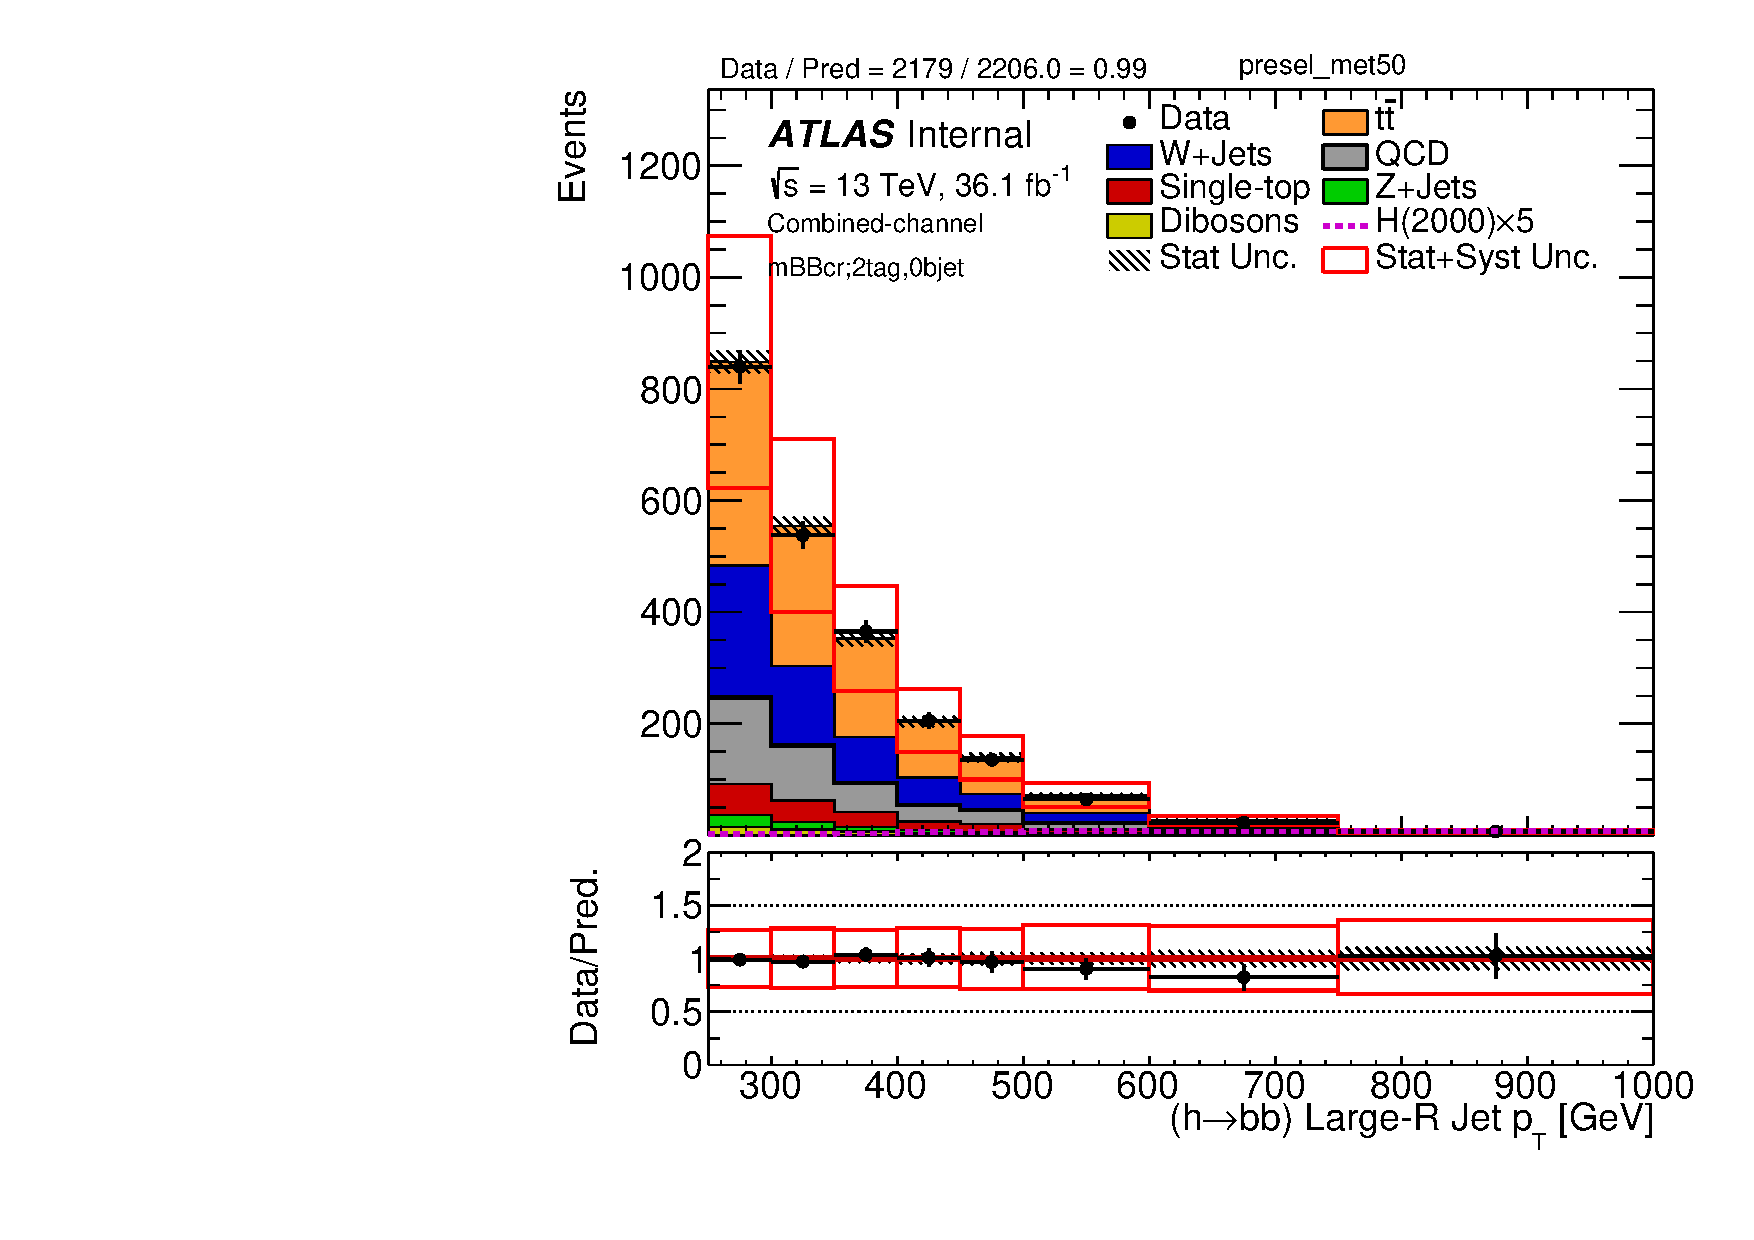
\includegraphics[width=0.49\textwidth]{./figures/boosted/PlotsInMbbCR/DataMC_2tag_0bjet_mbbcr_lepton_presel_met50_HbbPt}
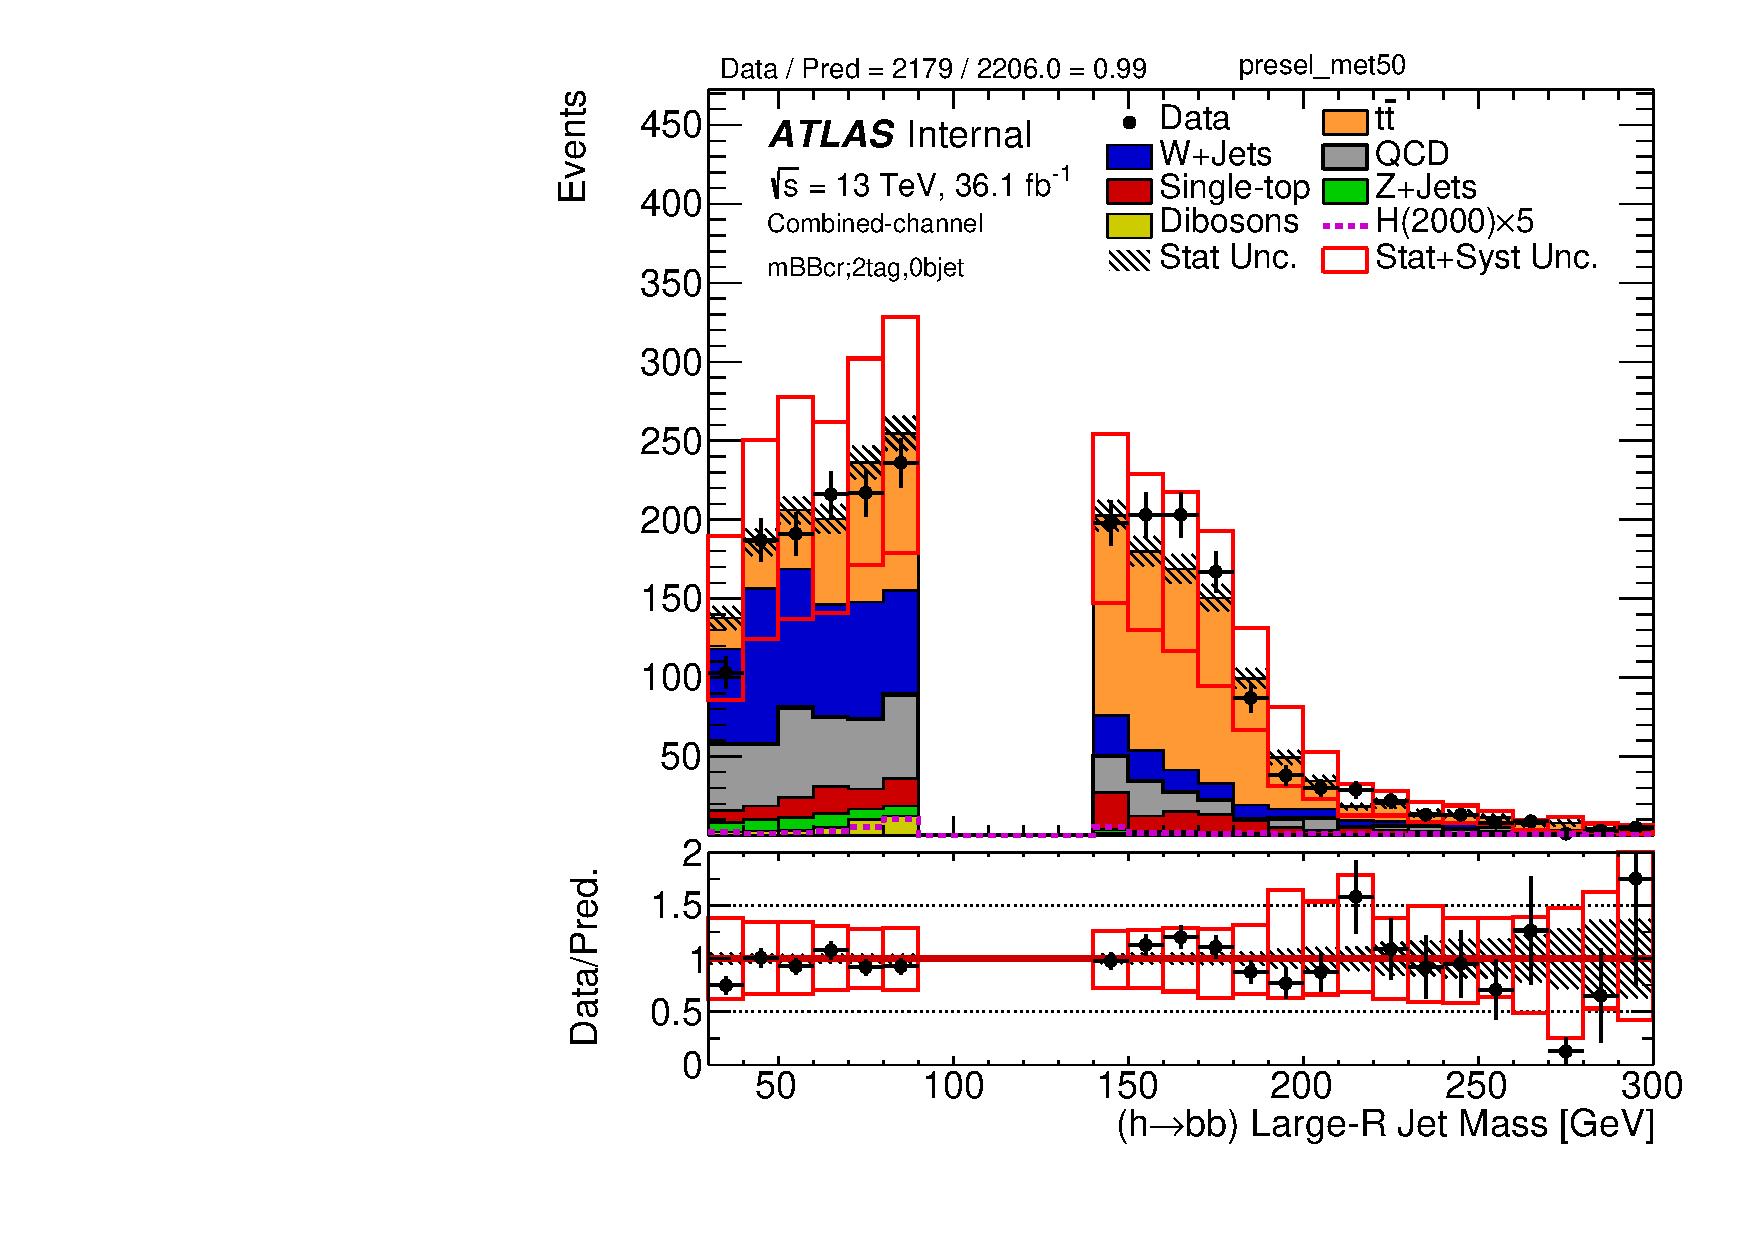
\includegraphics[width=0.49\textwidth]{./figures/boosted/PlotsInMbbCR/DataMC_2tag_0bjet_mbbcr_lepton_presel_met50_HbbMass} \\
\par\medskip
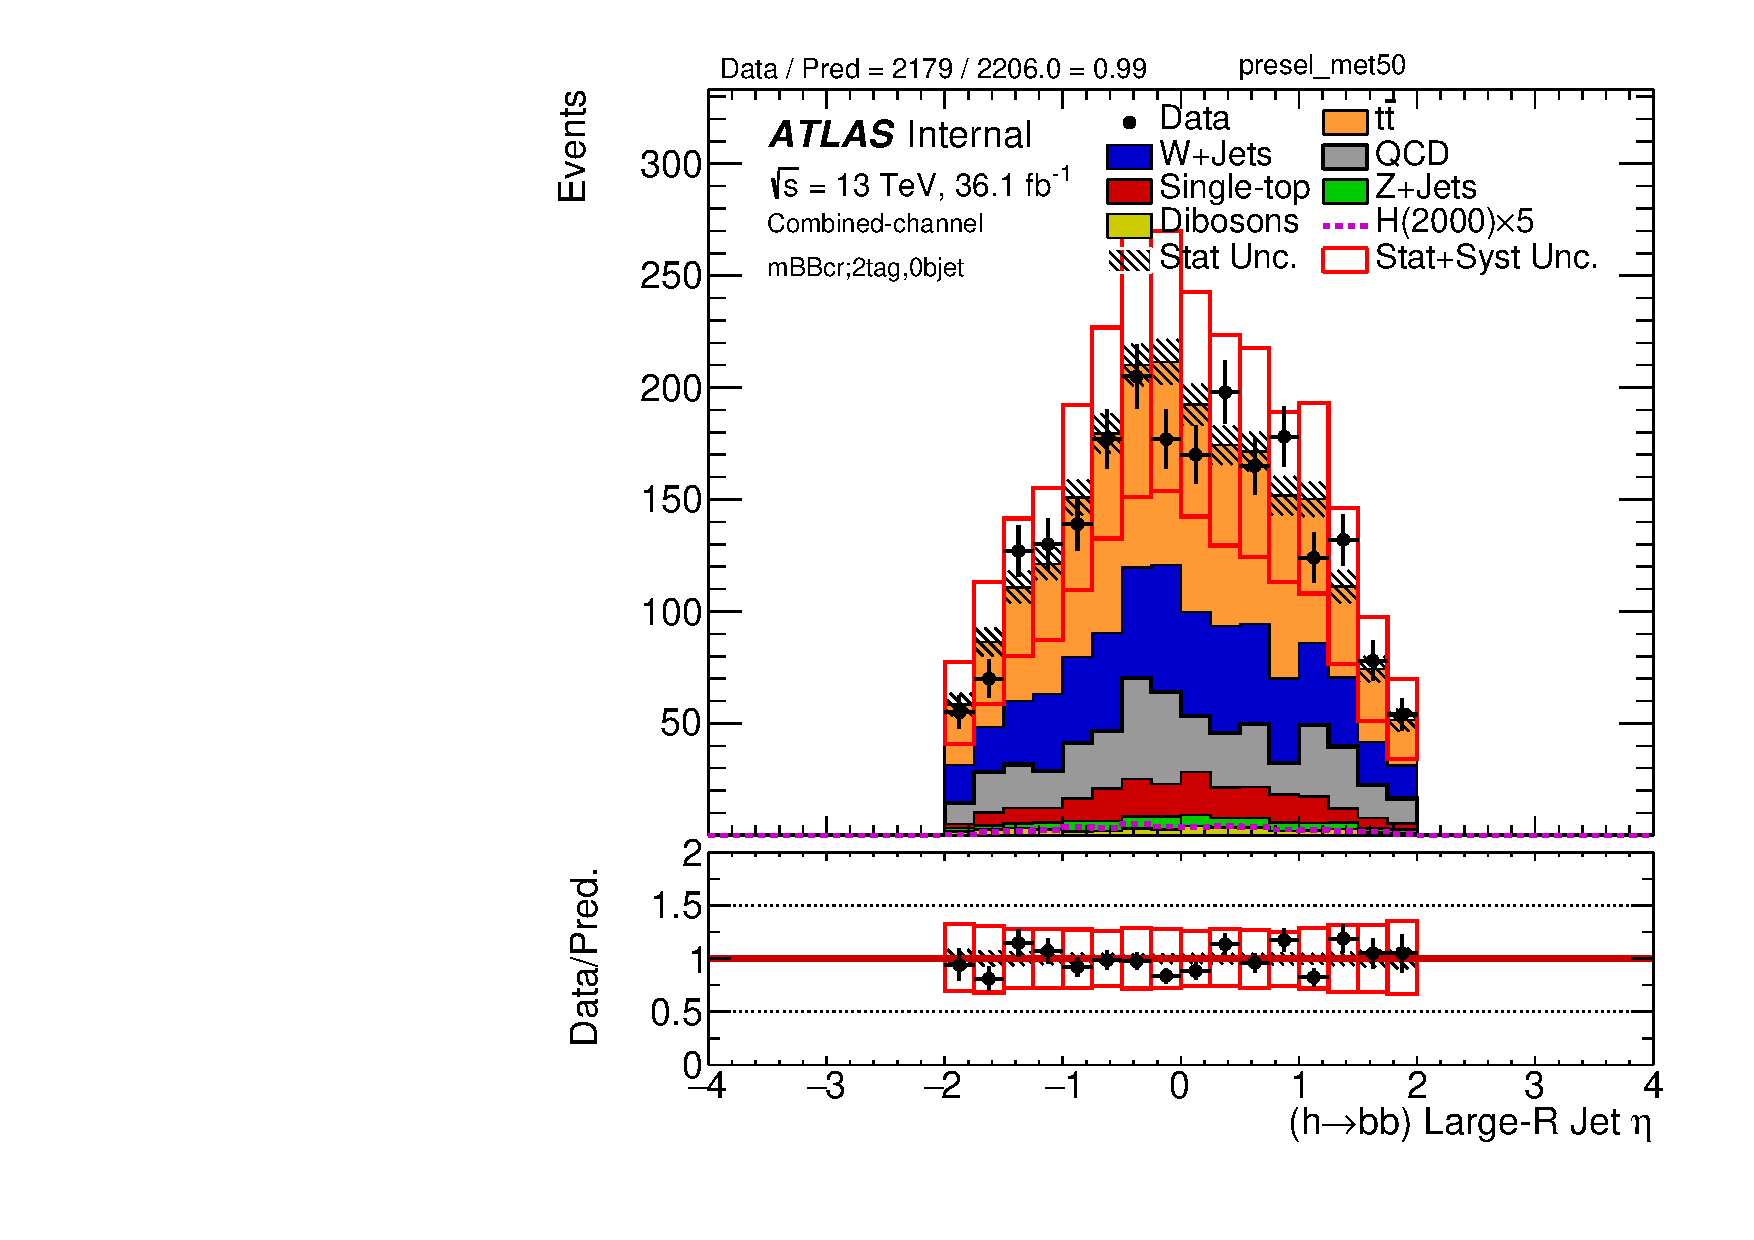
\includegraphics[width=0.49\textwidth]{./figures/boosted/PlotsInMbbCR/DataMC_2tag_0bjet_mbbcr_lepton_presel_met50_HbbEta} 
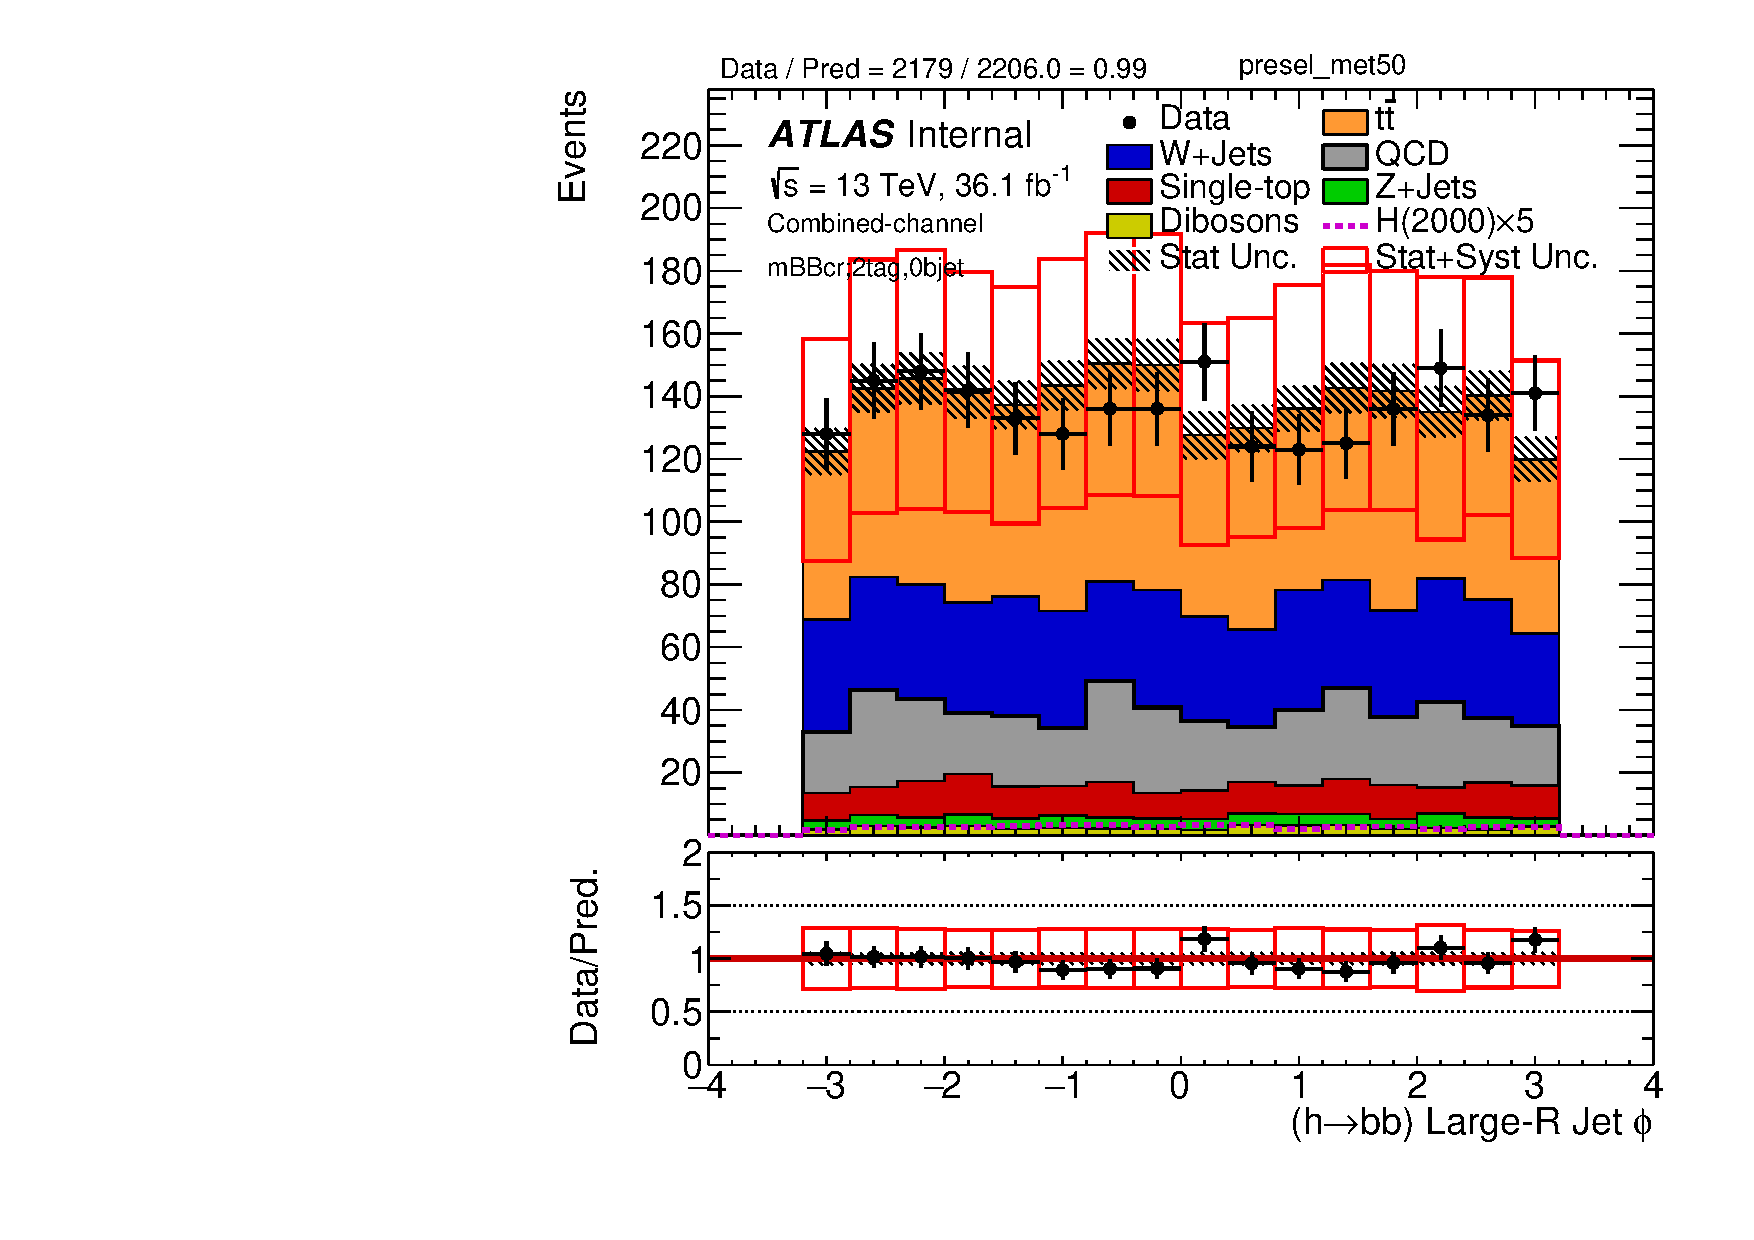
\includegraphics[width=0.49\textwidth]{./figures/boosted/PlotsInMbbCR/DataMC_2tag_0bjet_mbbcr_lepton_presel_met50_HbbPhi} 
\caption{Kinematic distributions of the reconstructed large-$R$ jet in the mBB control region (mBBcr).}
\label{fig:boosted_mbbcr_largerjet}
\end{center}
\end{figure}
\newpage
\begin{figure}[!h]
\begin{center}
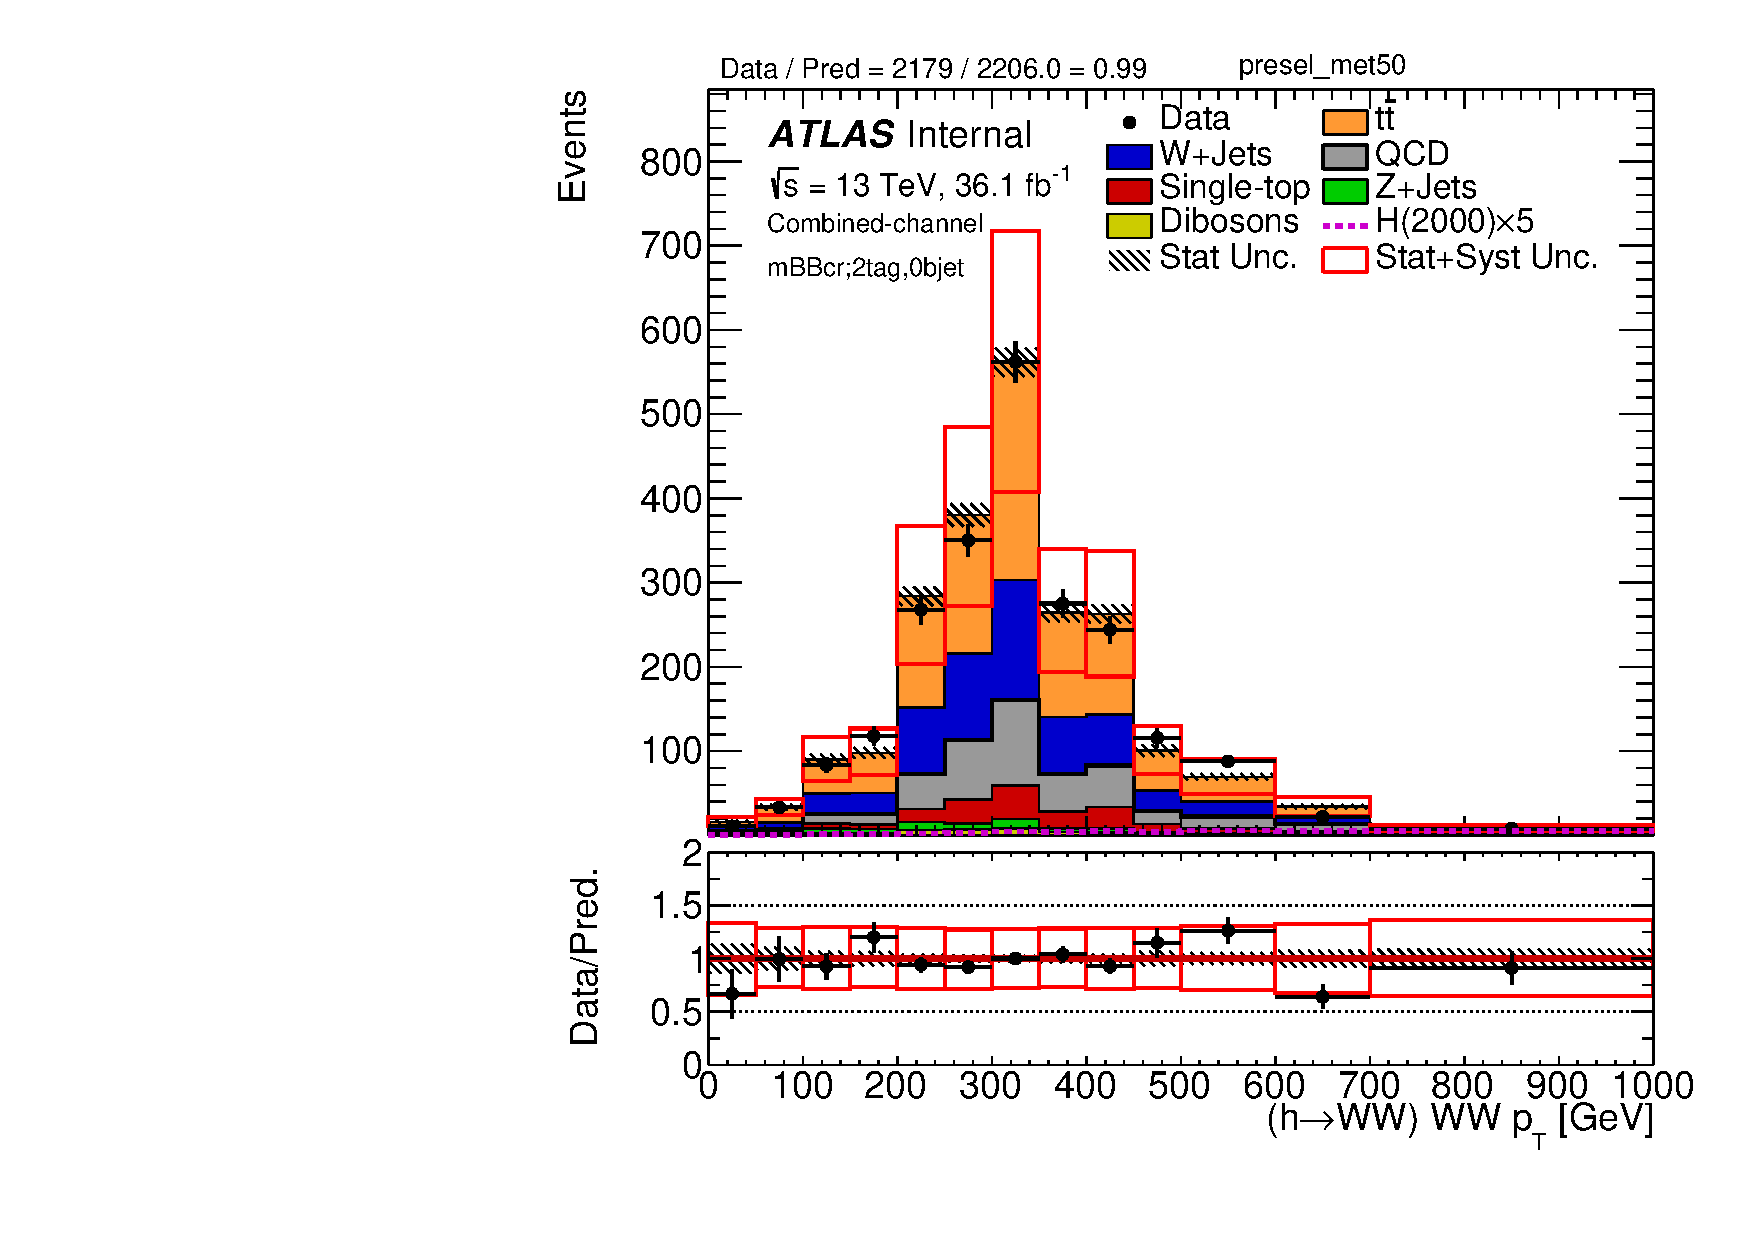
\includegraphics[width=0.49\textwidth]{./figures/boosted/PlotsInMbbCR/DataMC_2tag_0bjet_mbbcr_lepton_presel_met50_WWPt}
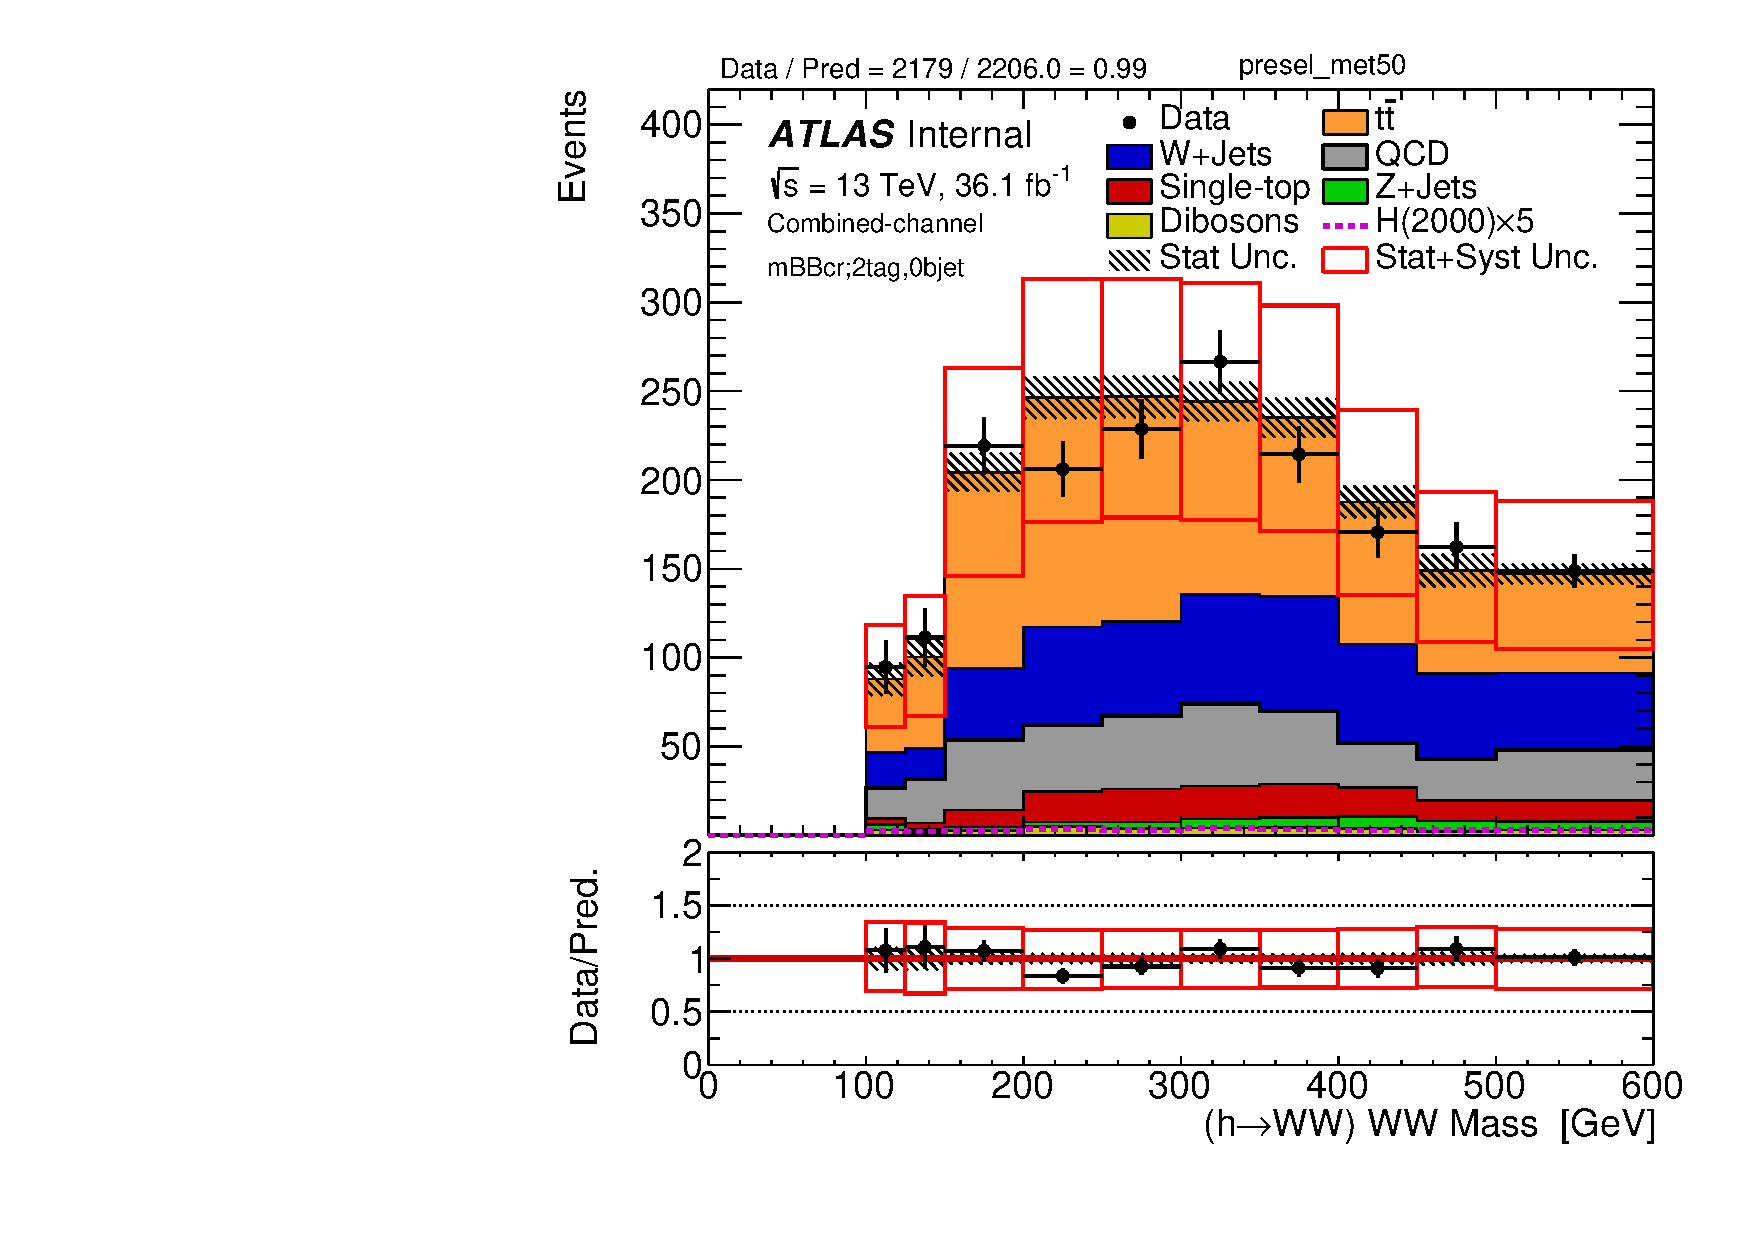
\includegraphics[width=0.49\textwidth]{./figures/boosted/PlotsInMbbCR/DataMC_2tag_0bjet_mbbcr_lepton_presel_met50_WWMass} \\
\par\medskip
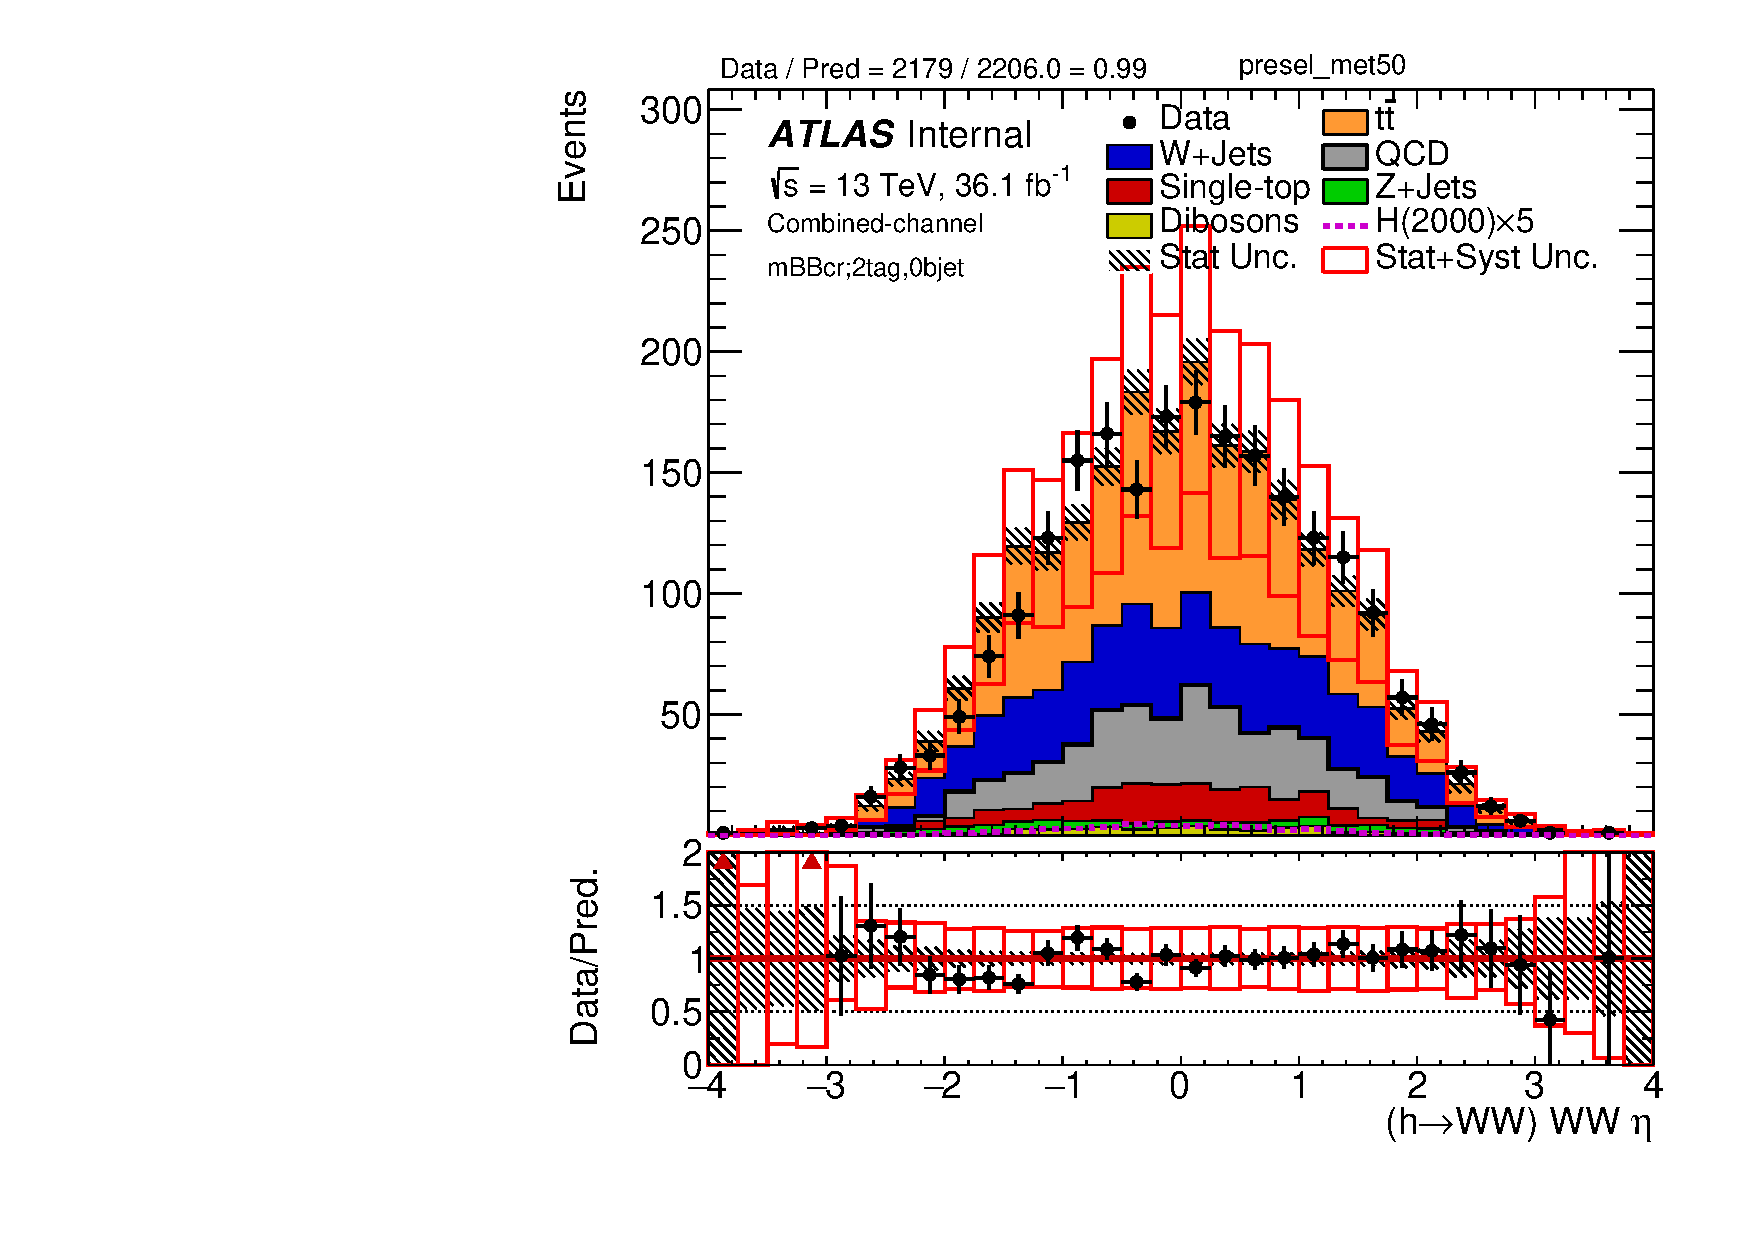
\includegraphics[width=0.49\textwidth]{./figures/boosted/PlotsInMbbCR/DataMC_2tag_0bjet_mbbcr_lepton_presel_met50_WWEta}
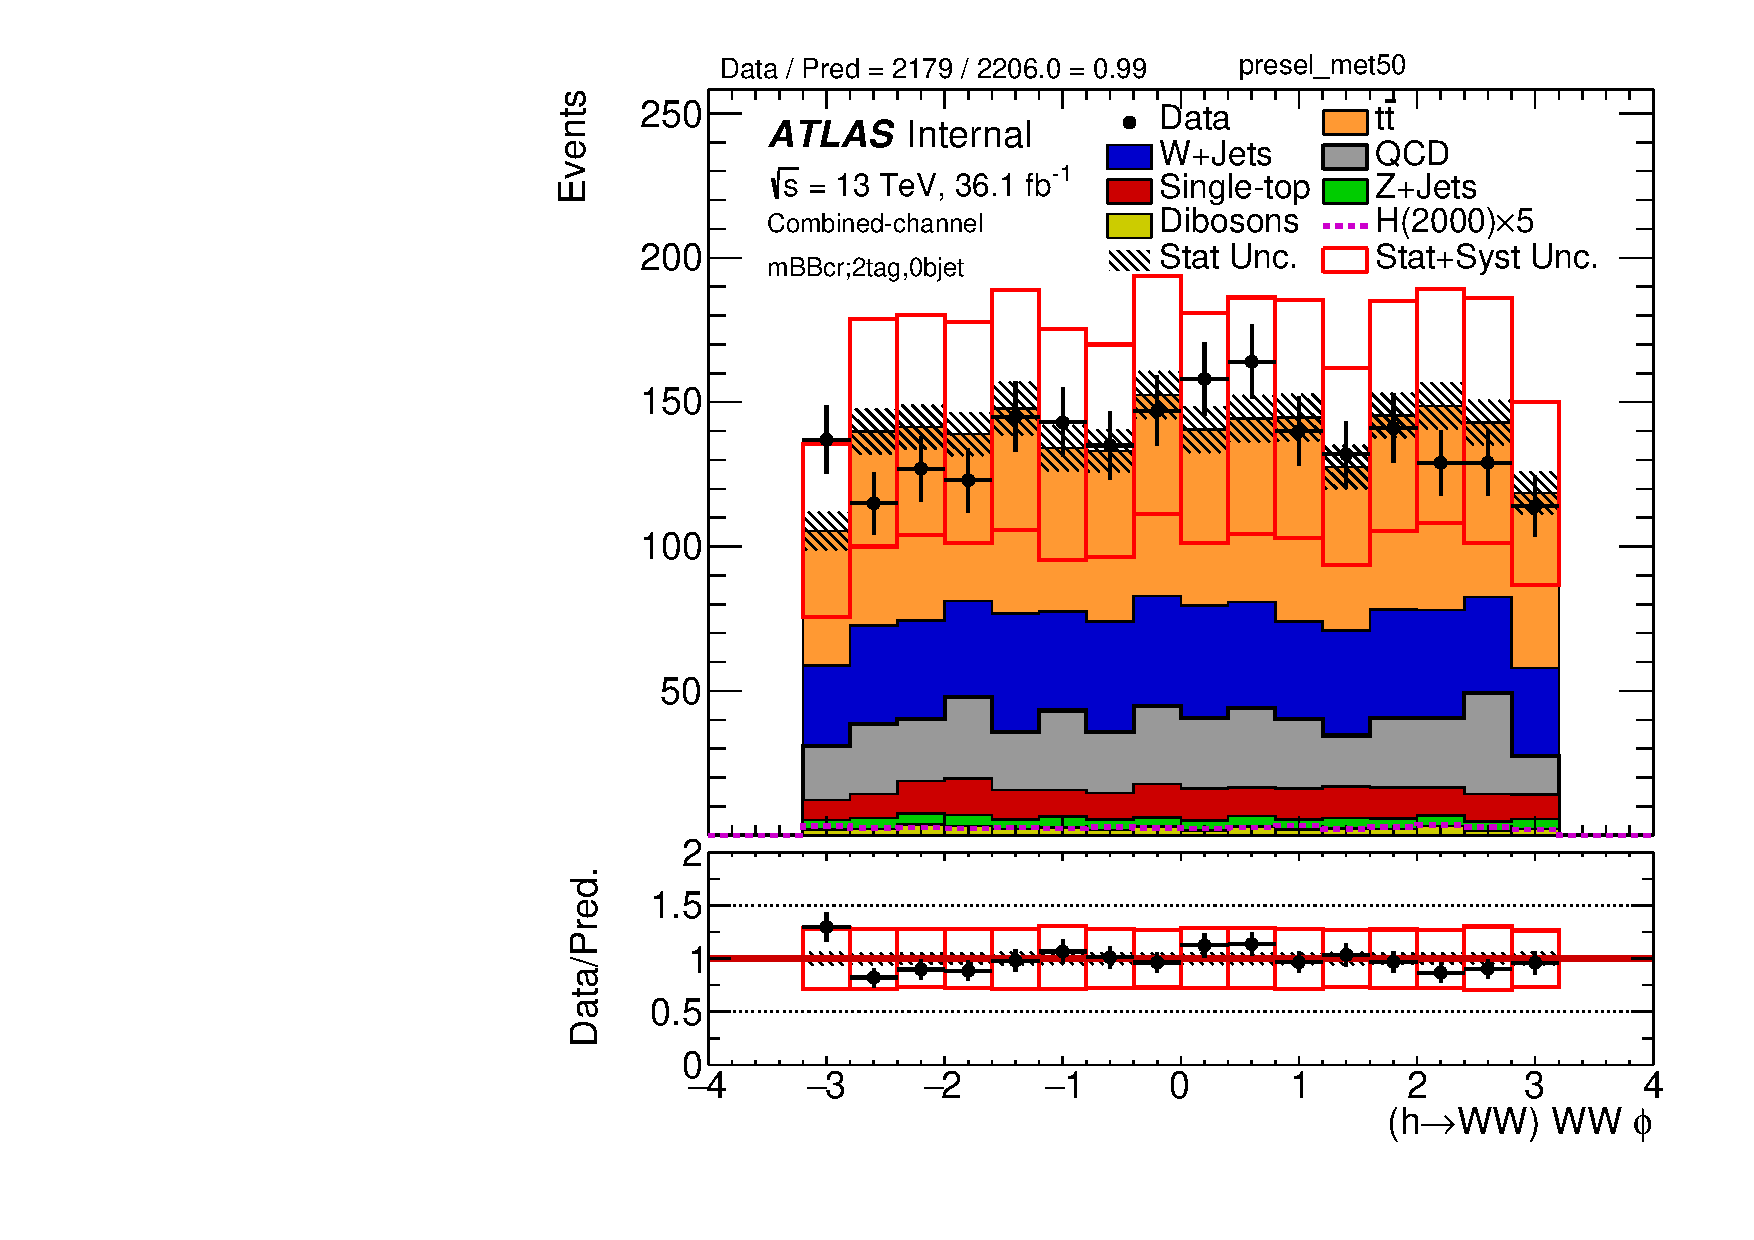
\includegraphics[width=0.49\textwidth]{./figures/boosted/PlotsInMbbCR/DataMC_2tag_0bjet_mbbcr_lepton_presel_met50_WWPhi}
\caption{Kinematic distributions of the reconstructed $h \to WW$ system in the mBB control region (mBBcr).}
\label{fig:boosted_mbbcr_wwsystem}
\end{center}
\end{figure}
 \newpage
\begin{figure}[!h]
\begin{center}
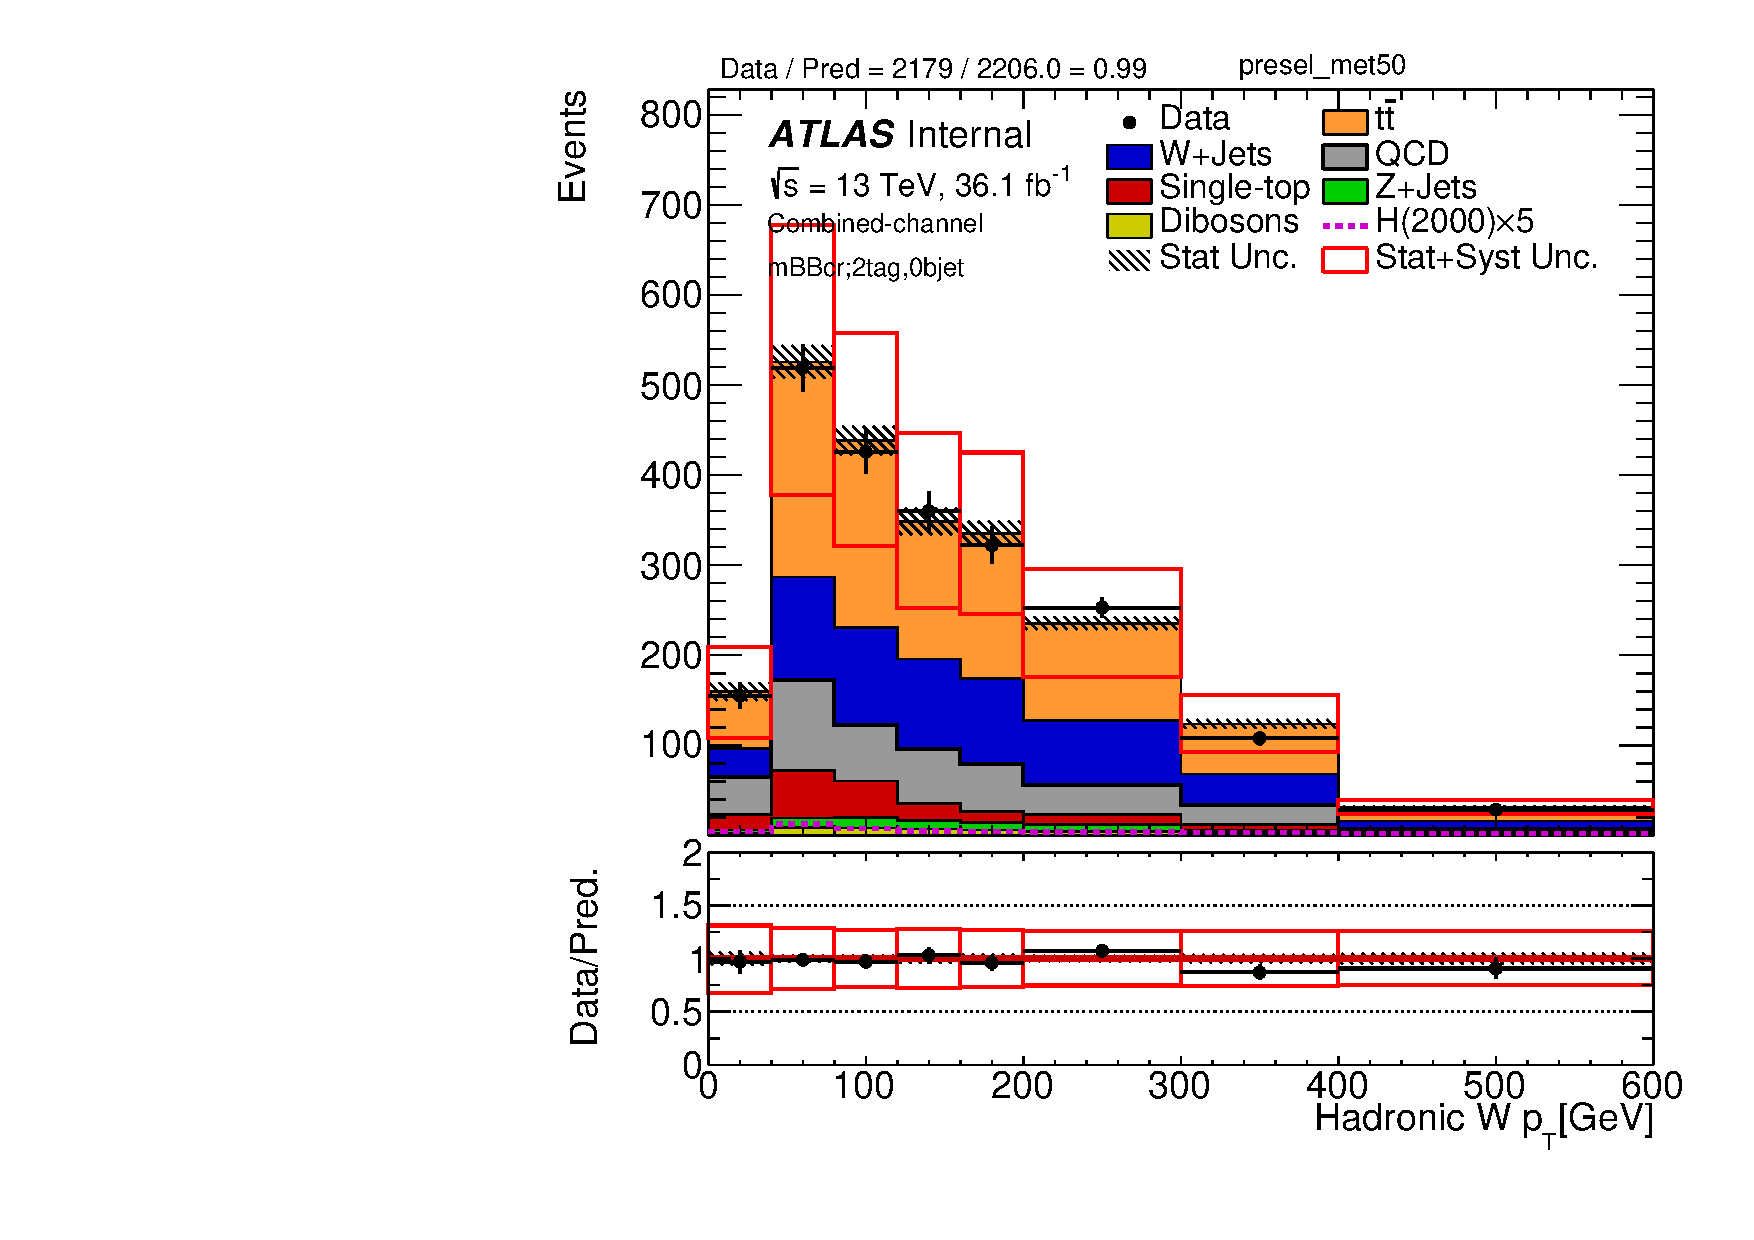
\includegraphics[width=0.49\textwidth]{./figures/boosted/PlotsInMbbCR/DataMC_2tag_0bjet_mbbcr_lepton_presel_met50_WhadPt}
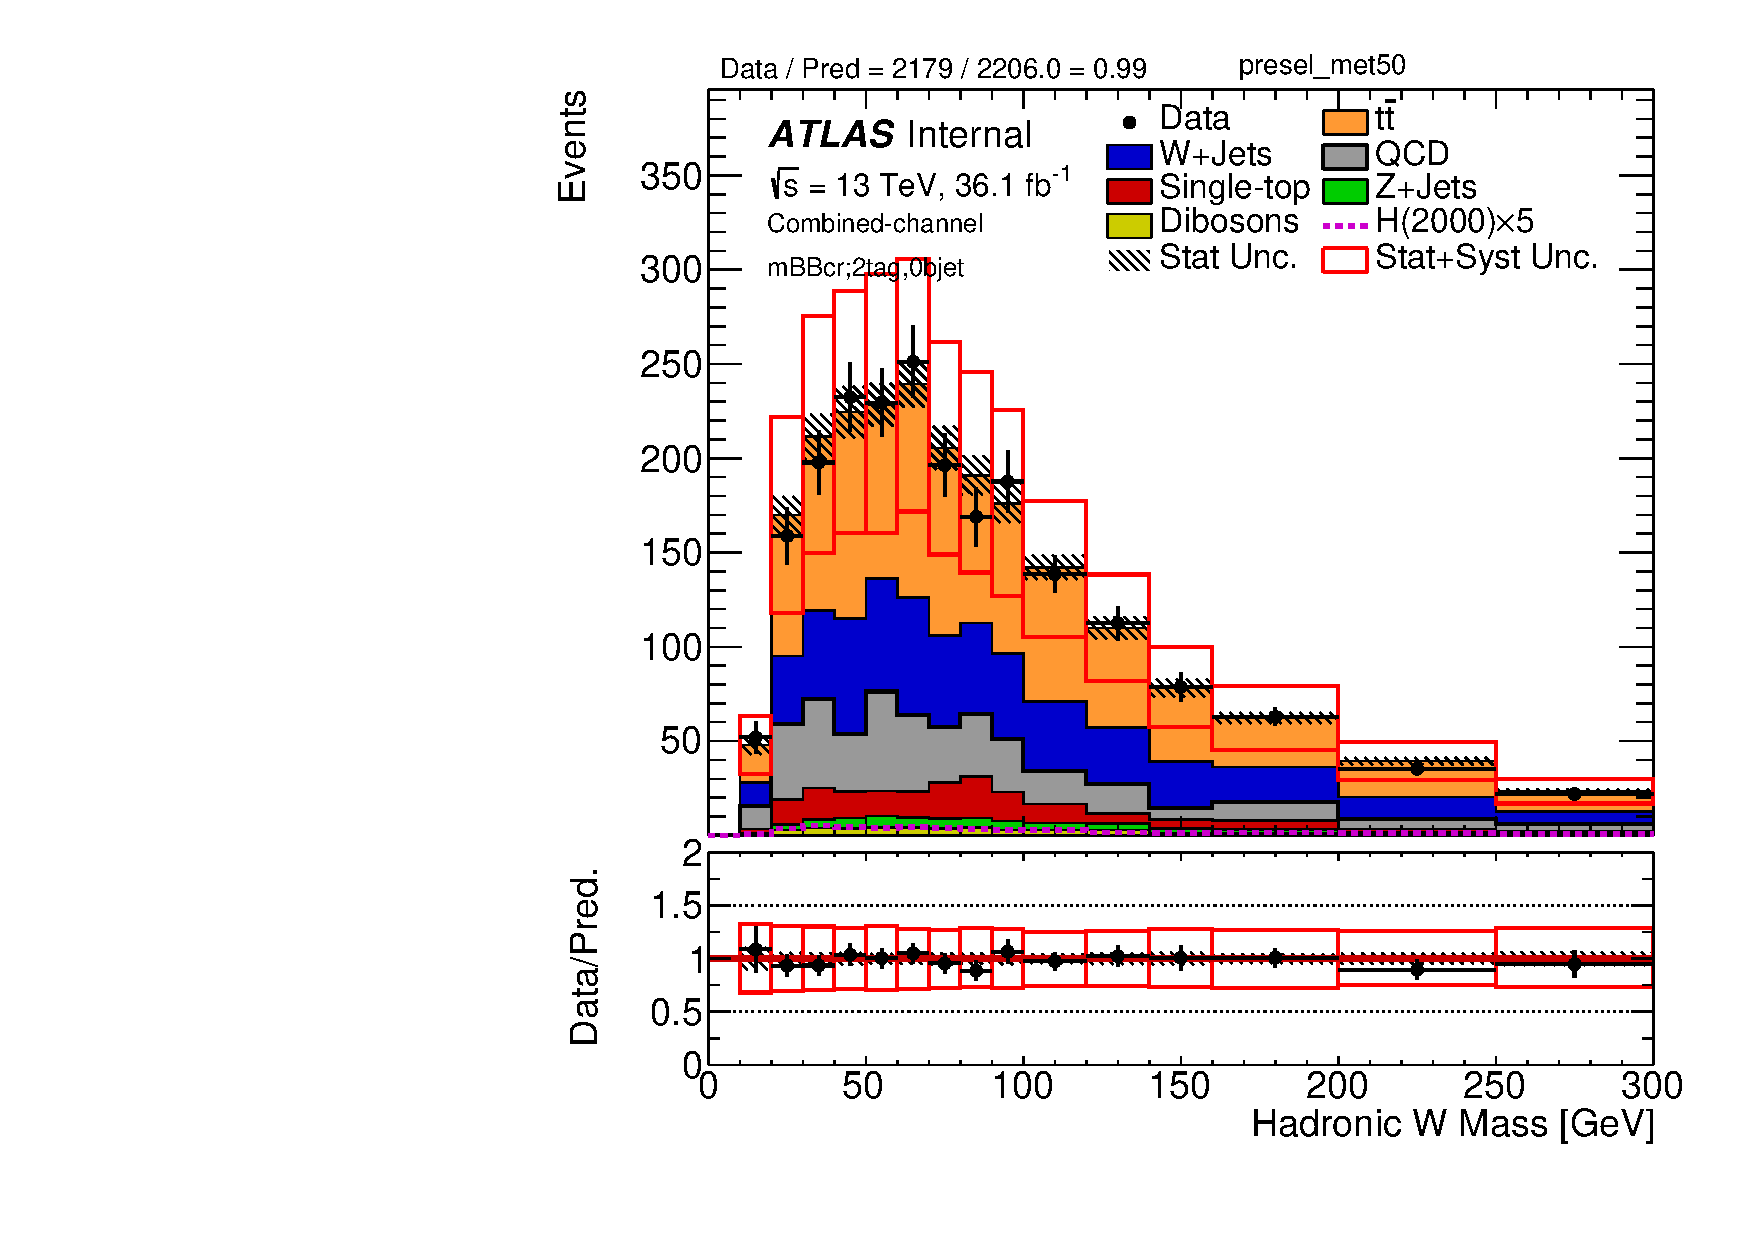
\includegraphics[width=0.49\textwidth]{./figures/boosted/PlotsInMbbCR/DataMC_2tag_0bjet_mbbcr_lepton_presel_met50_WhadMass} \\
\par\medskip
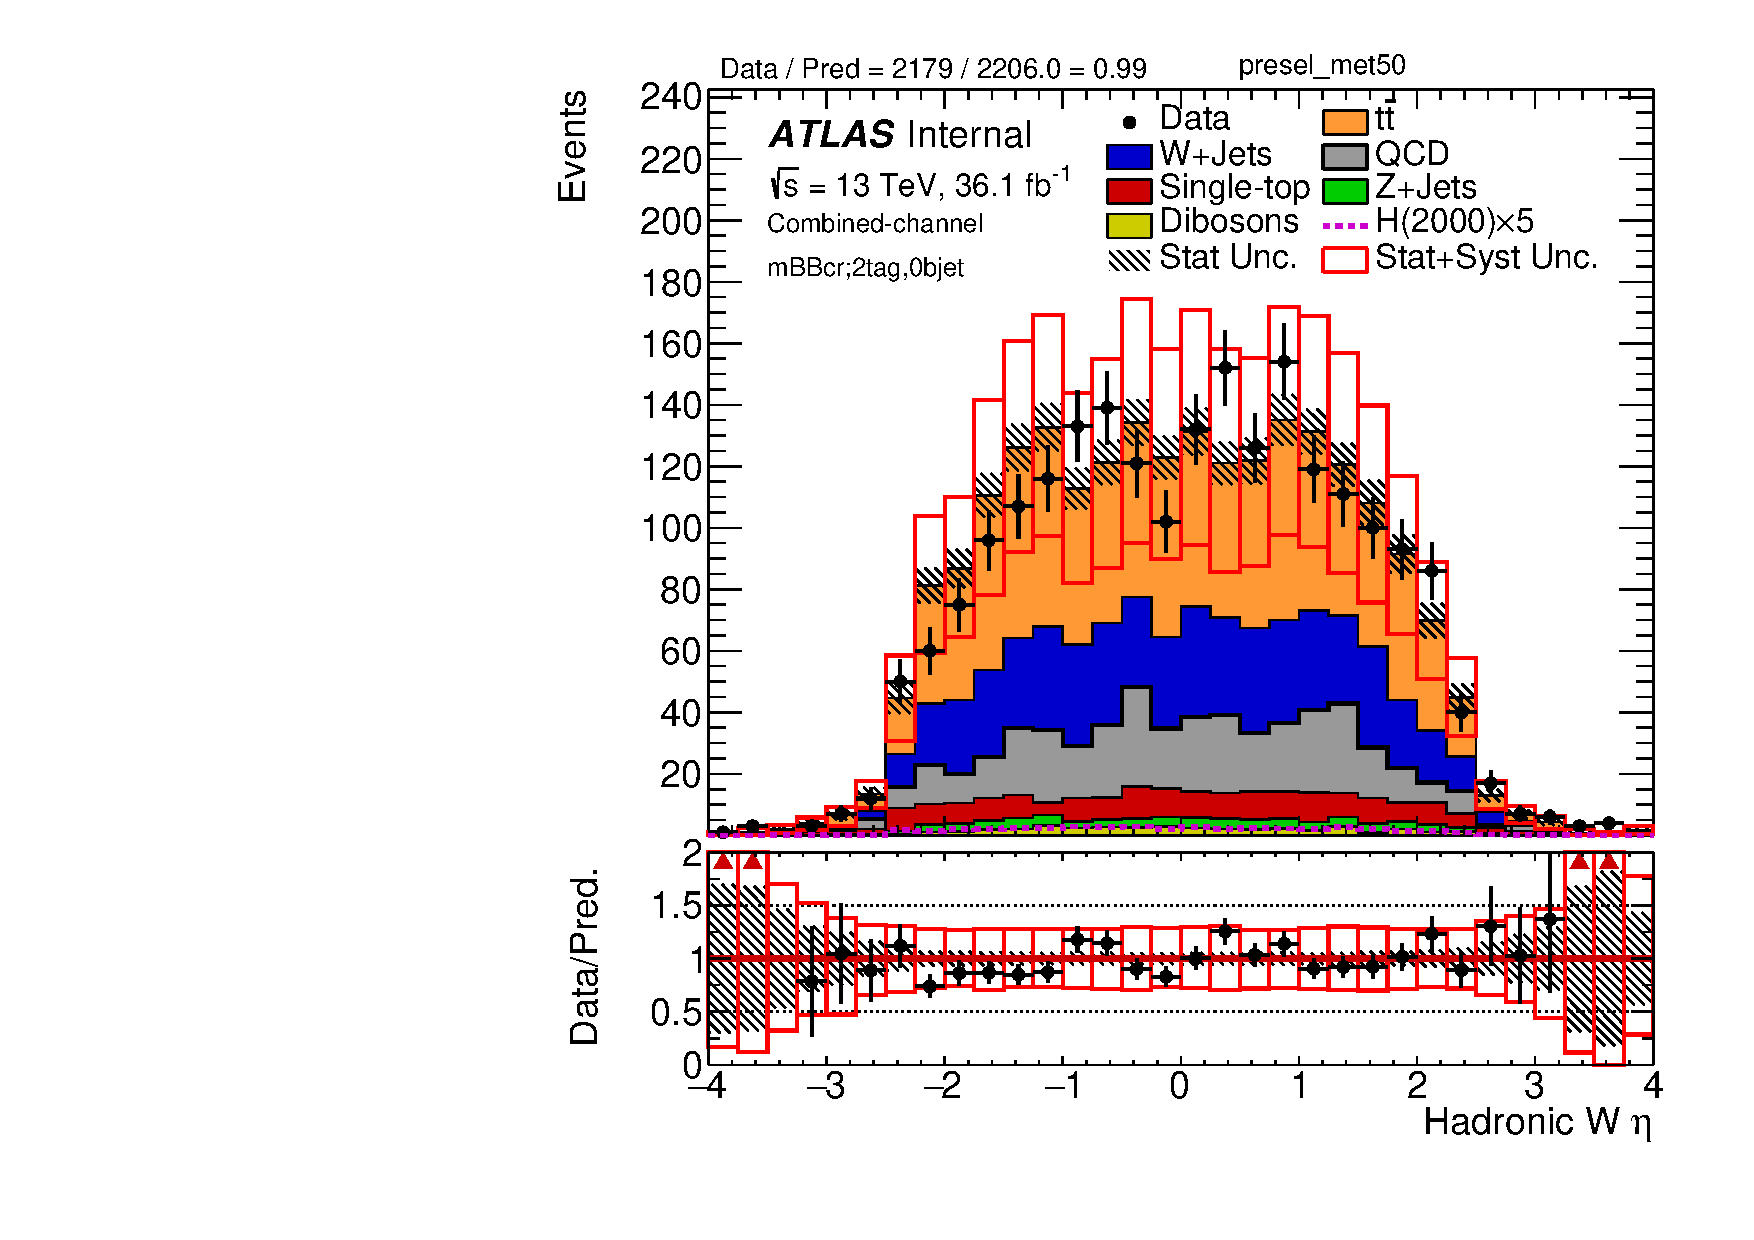
\includegraphics[width=0.49\textwidth]{./figures/boosted/PlotsInMbbCR/DataMC_2tag_0bjet_mbbcr_lepton_presel_met50_WhadEta}
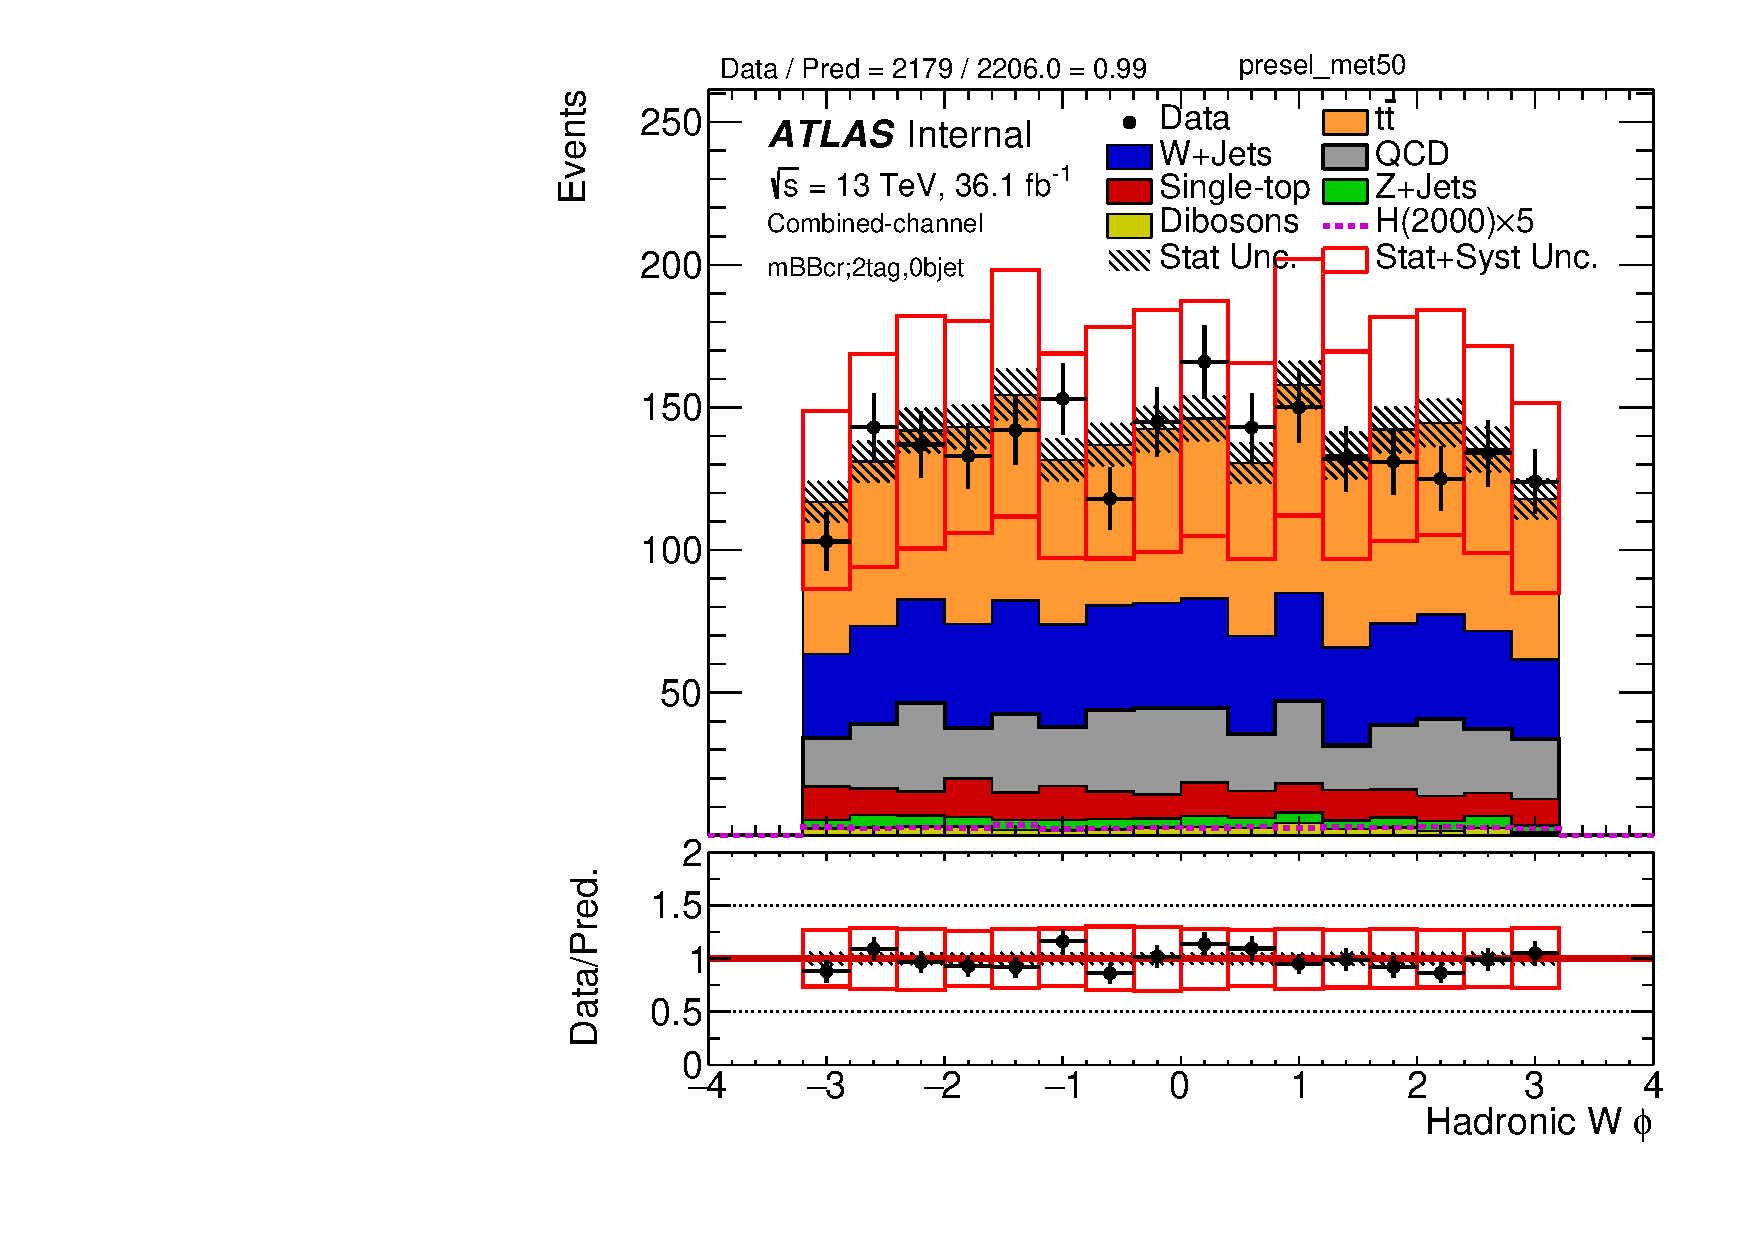
\includegraphics[width=0.49\textwidth]{./figures/boosted/PlotsInMbbCR/DataMC_2tag_0bjet_mbbcr_lepton_presel_met50_WhadPhi}
\caption{Kinematic distributions of the reconstructed $W \to q\bar{q}$ system in the mBB control region (mBBcr).}
\label{fig:boosted_mbbcr_whad}
\end{center}
\end{figure}
 \newpage
\begin{figure}[!h]
\begin{center}
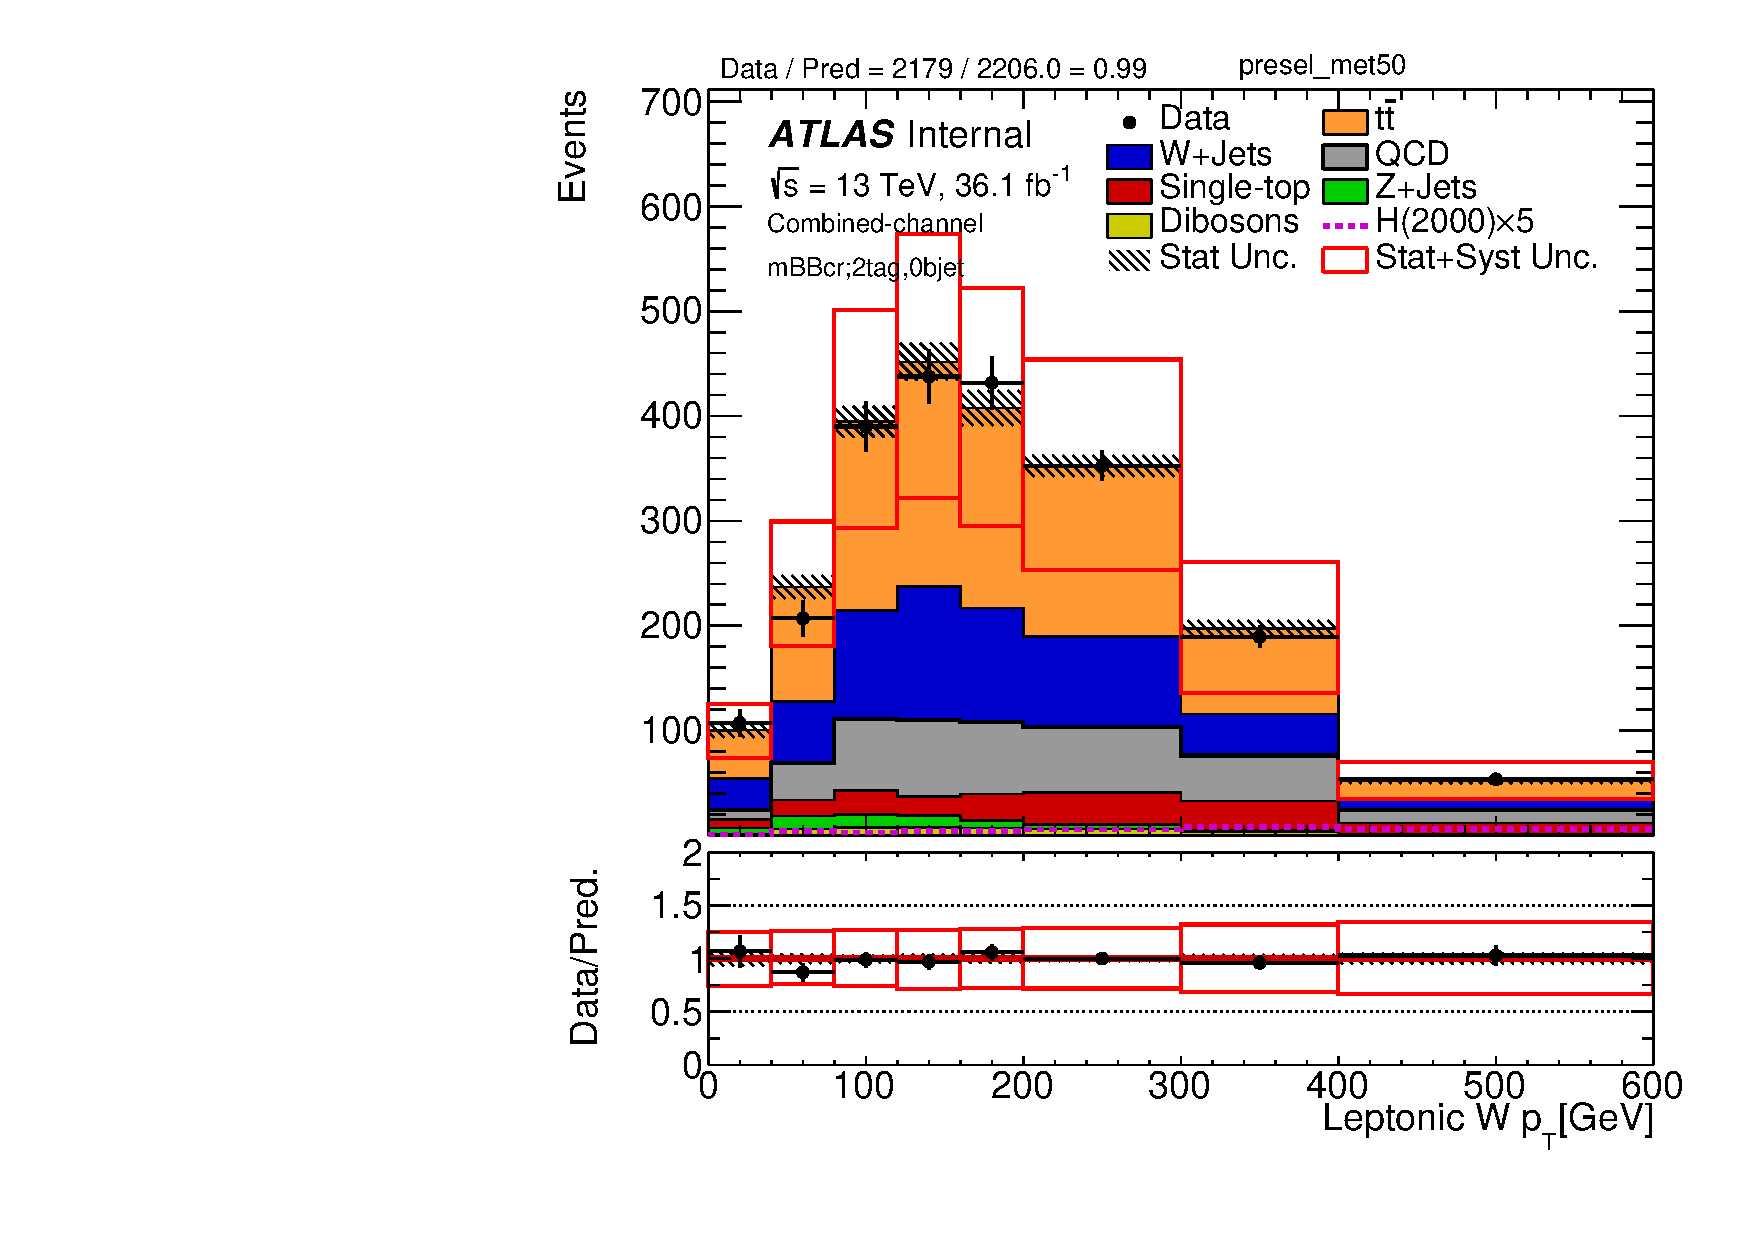
\includegraphics[width=0.49\textwidth]{./figures/boosted/PlotsInMbbCR/DataMC_2tag_0bjet_mbbcr_lepton_presel_met50_WlepPt}
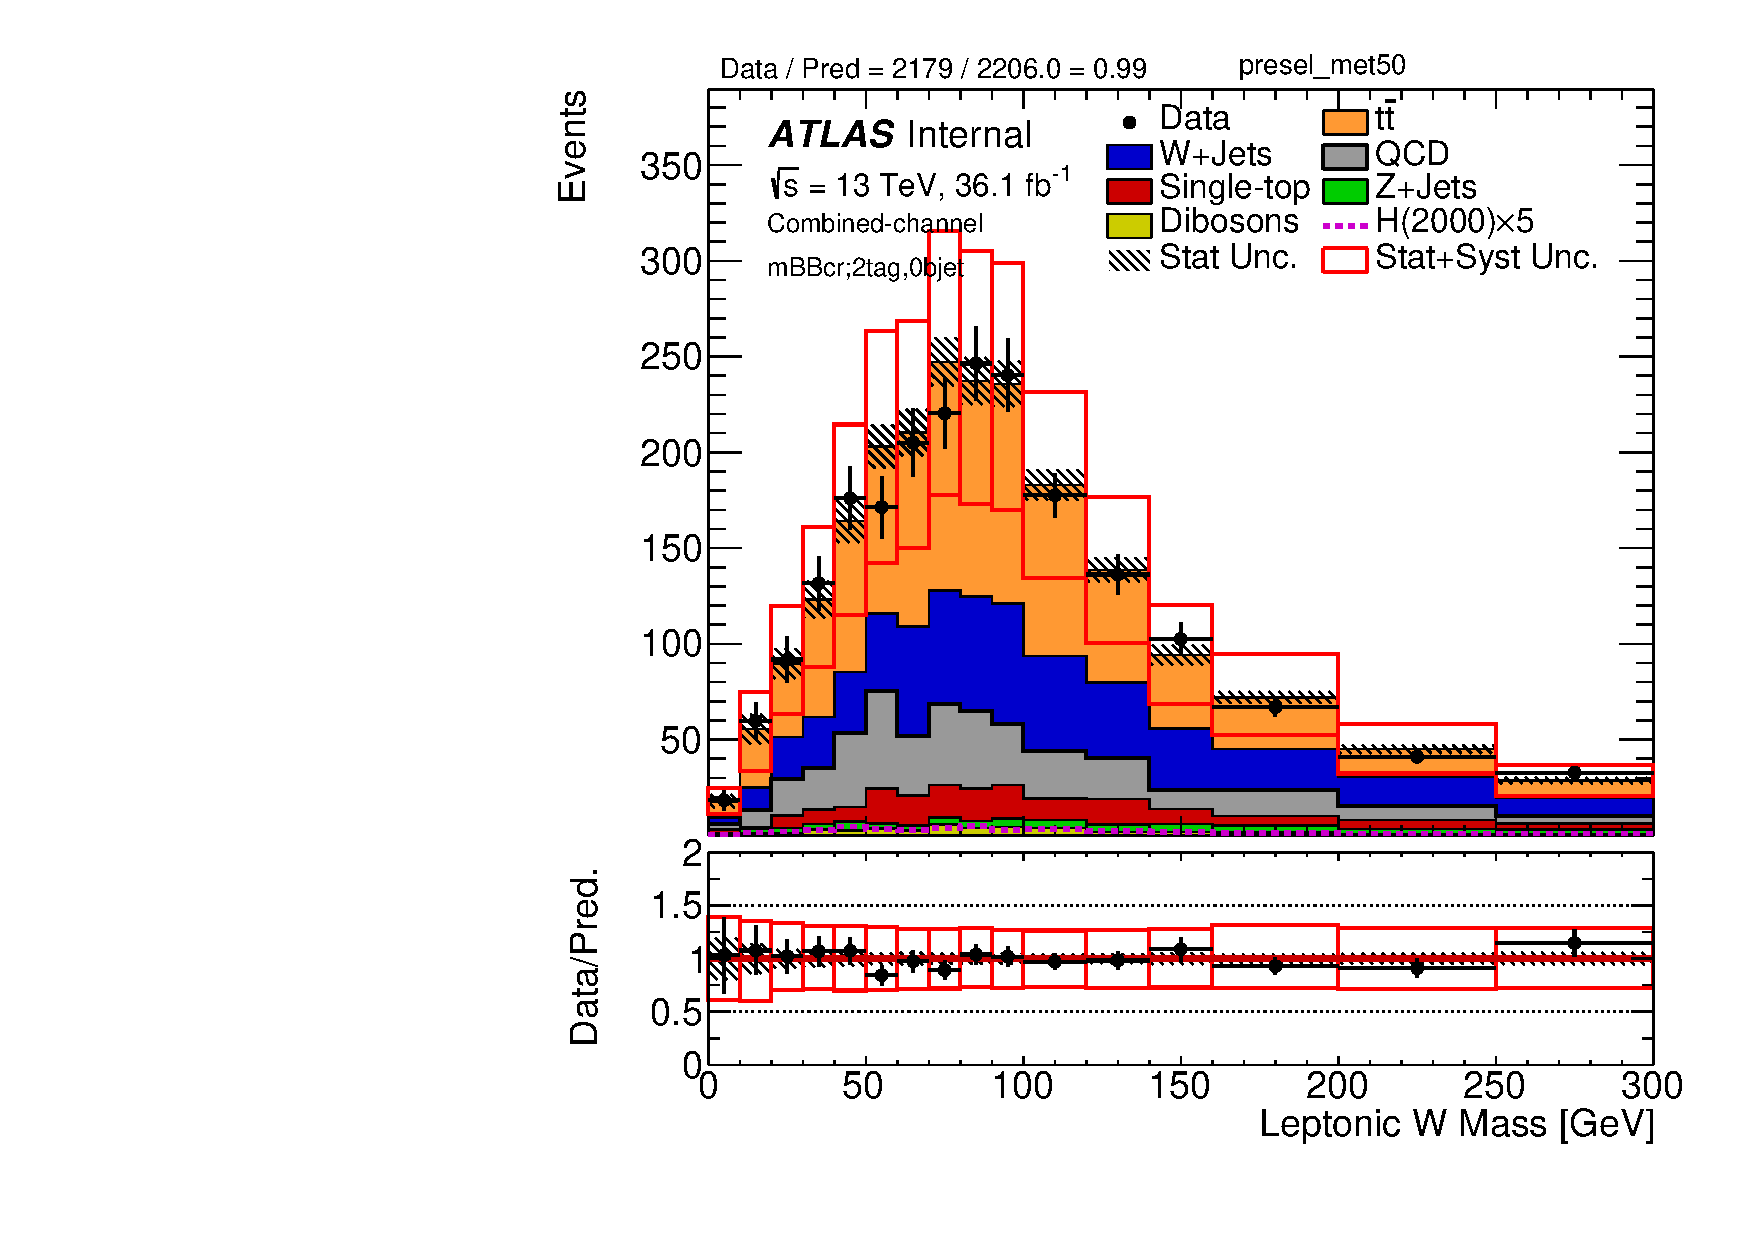
\includegraphics[width=0.49\textwidth]{./figures/boosted/PlotsInMbbCR/DataMC_2tag_0bjet_mbbcr_lepton_presel_met50_WlepMass} \\
\par\medskip
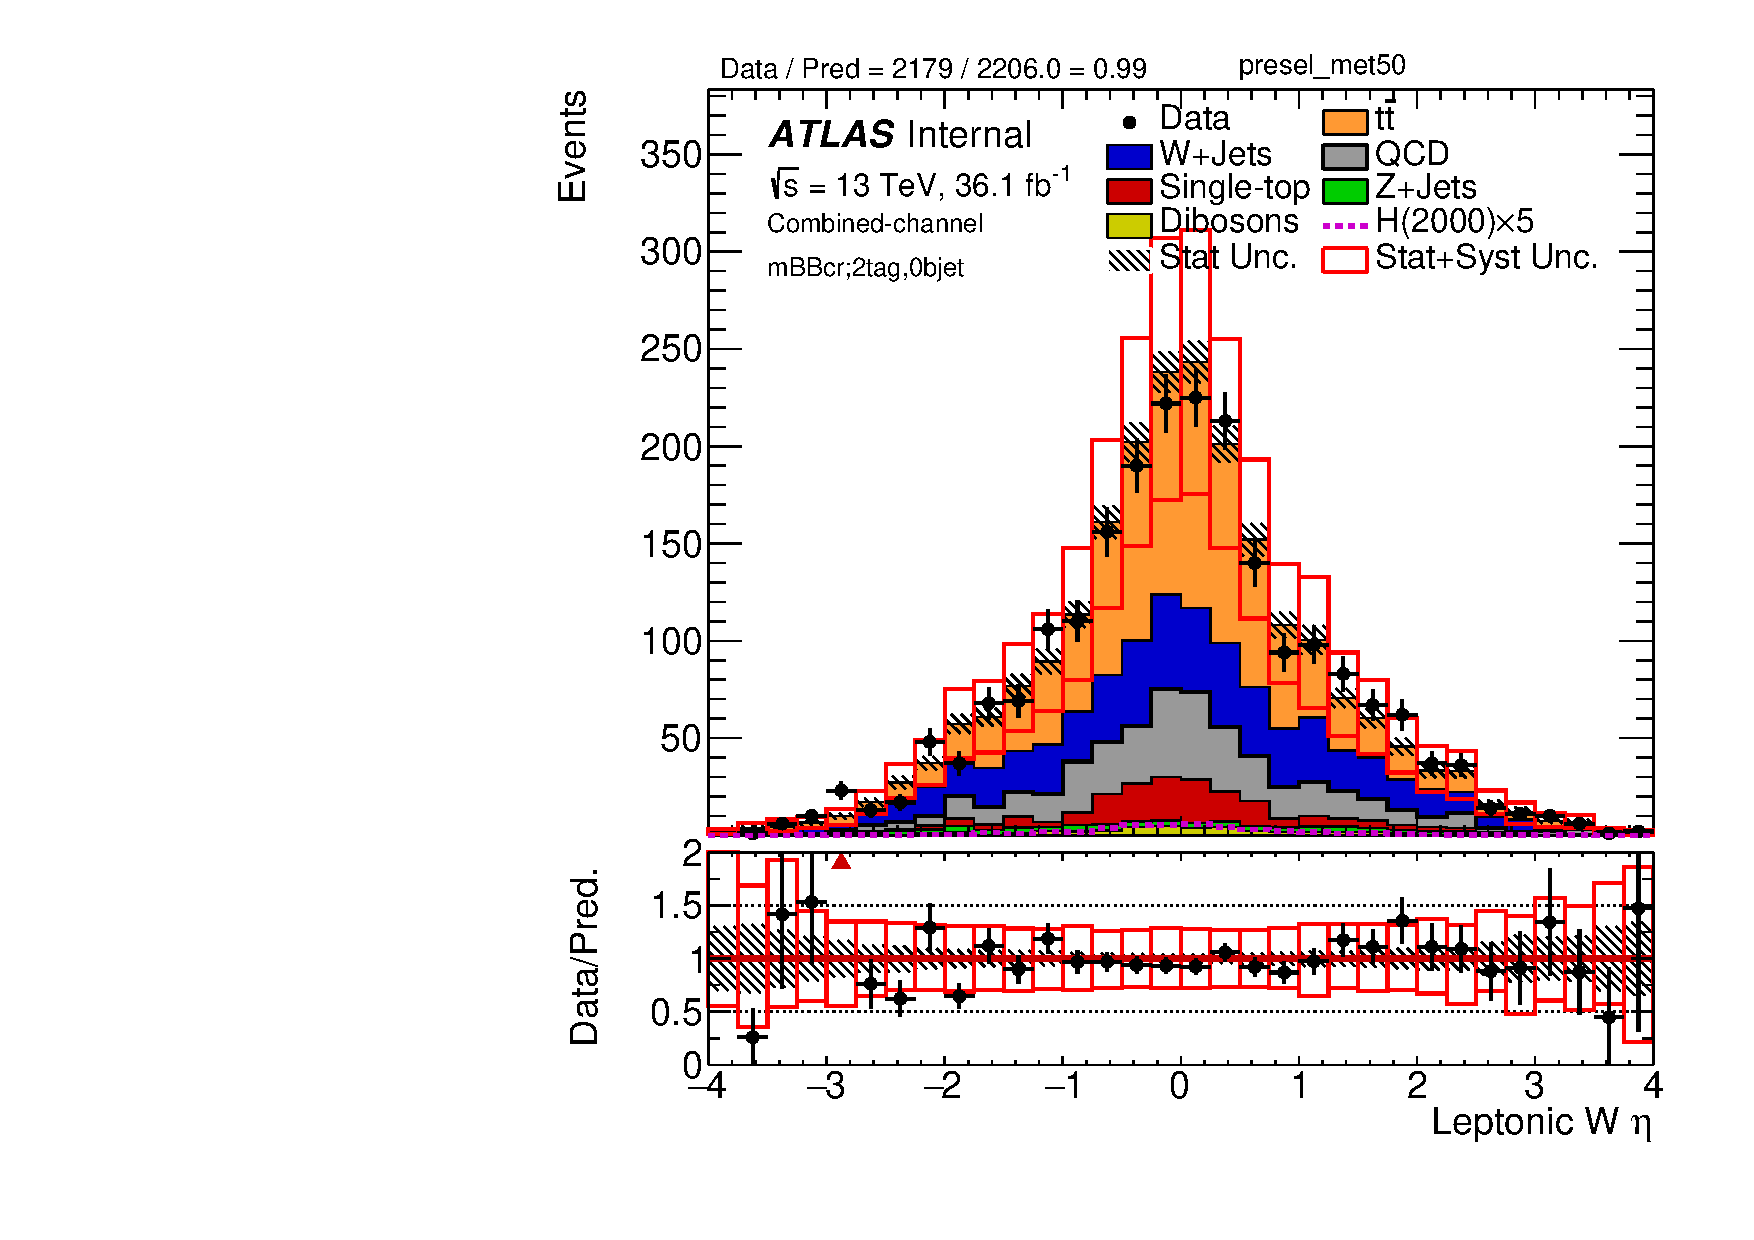
\includegraphics[width=0.49\textwidth]{./figures/boosted/PlotsInMbbCR/DataMC_2tag_0bjet_mbbcr_lepton_presel_met50_WlepEta}
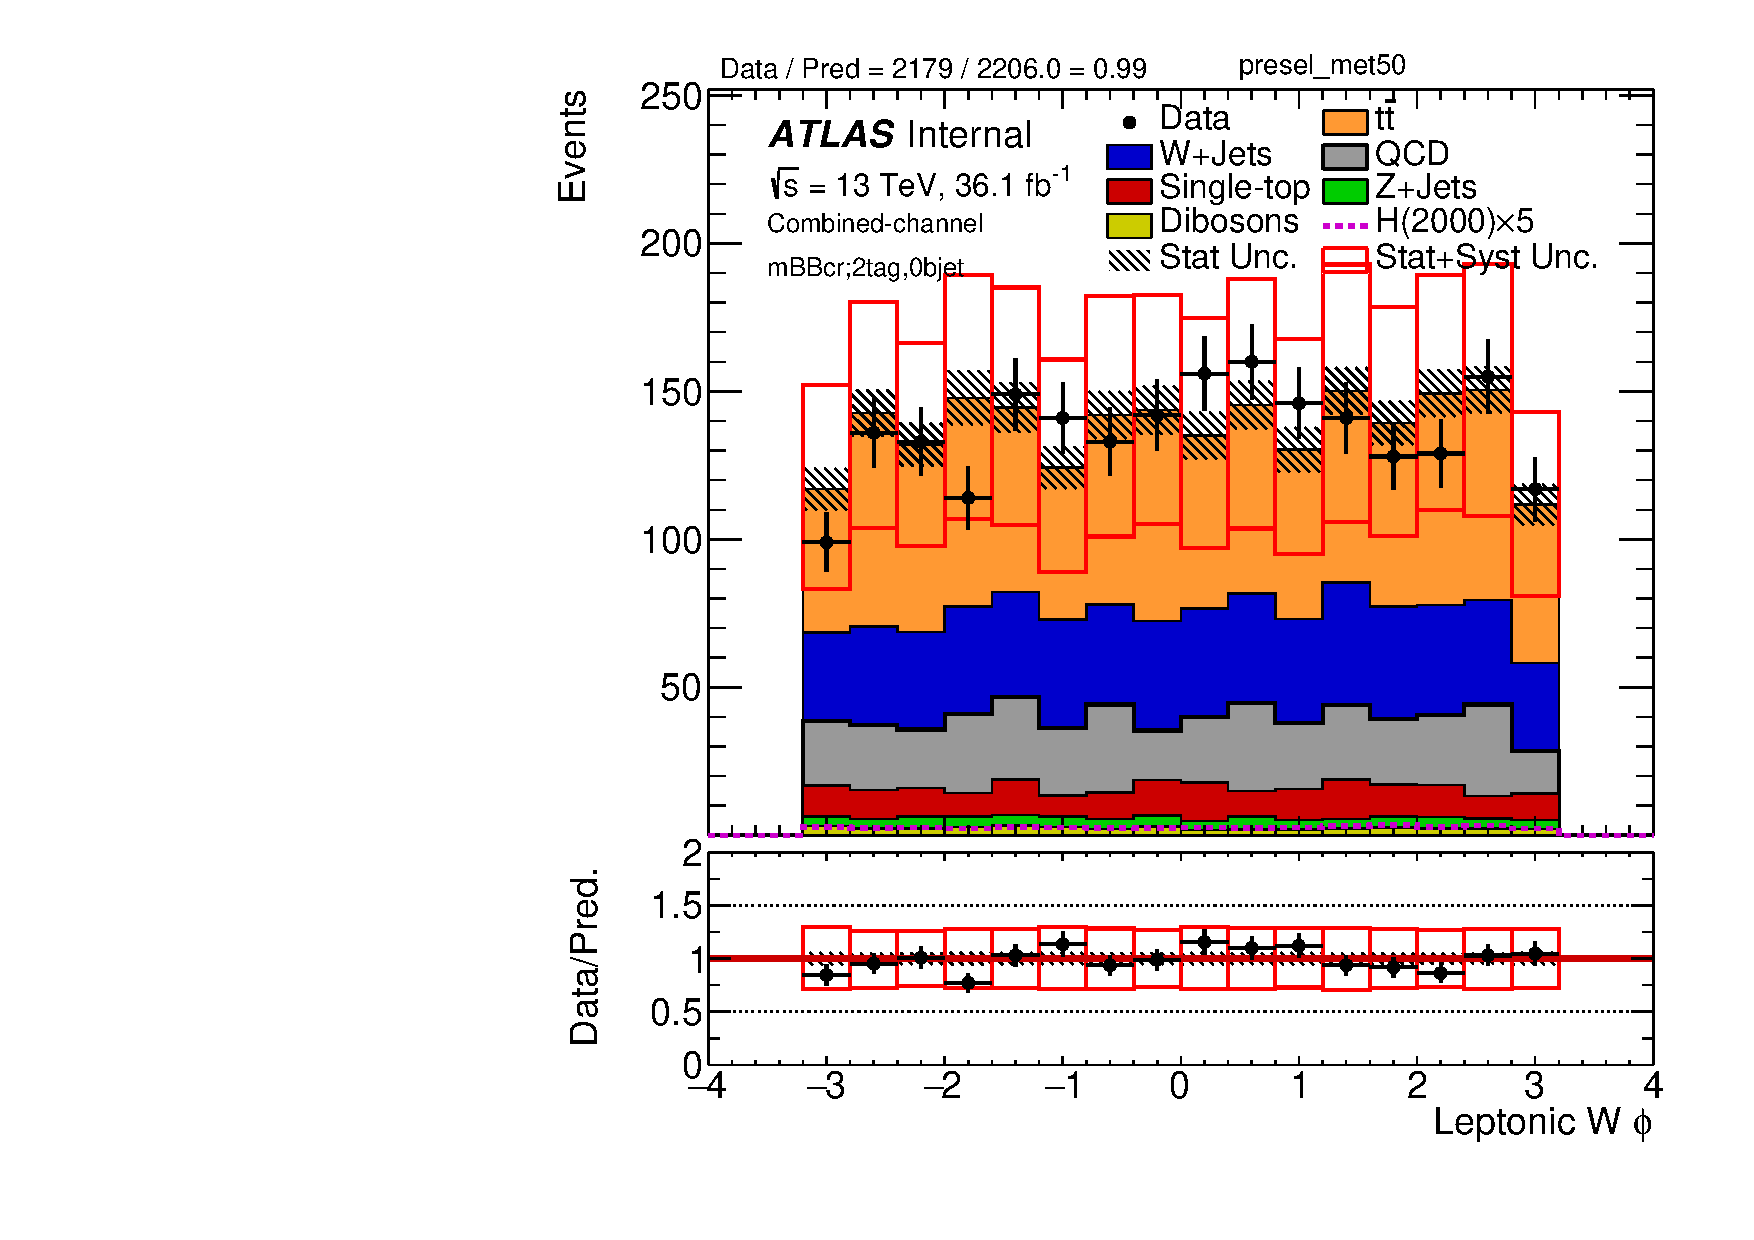
\includegraphics[width=0.49\textwidth]{./figures/boosted/PlotsInMbbCR/DataMC_2tag_0bjet_mbbcr_lepton_presel_met50_WlepPhi}
\caption{Kinematic distributions of the reconstructed $W \to l\nu$ system in the mBB control region (mBBcr).}
\label{fig:boosted_mbbcr_wlep}
\end{center}
\end{figure}
 \newpage
\begin{figure}[!h]
\begin{center}
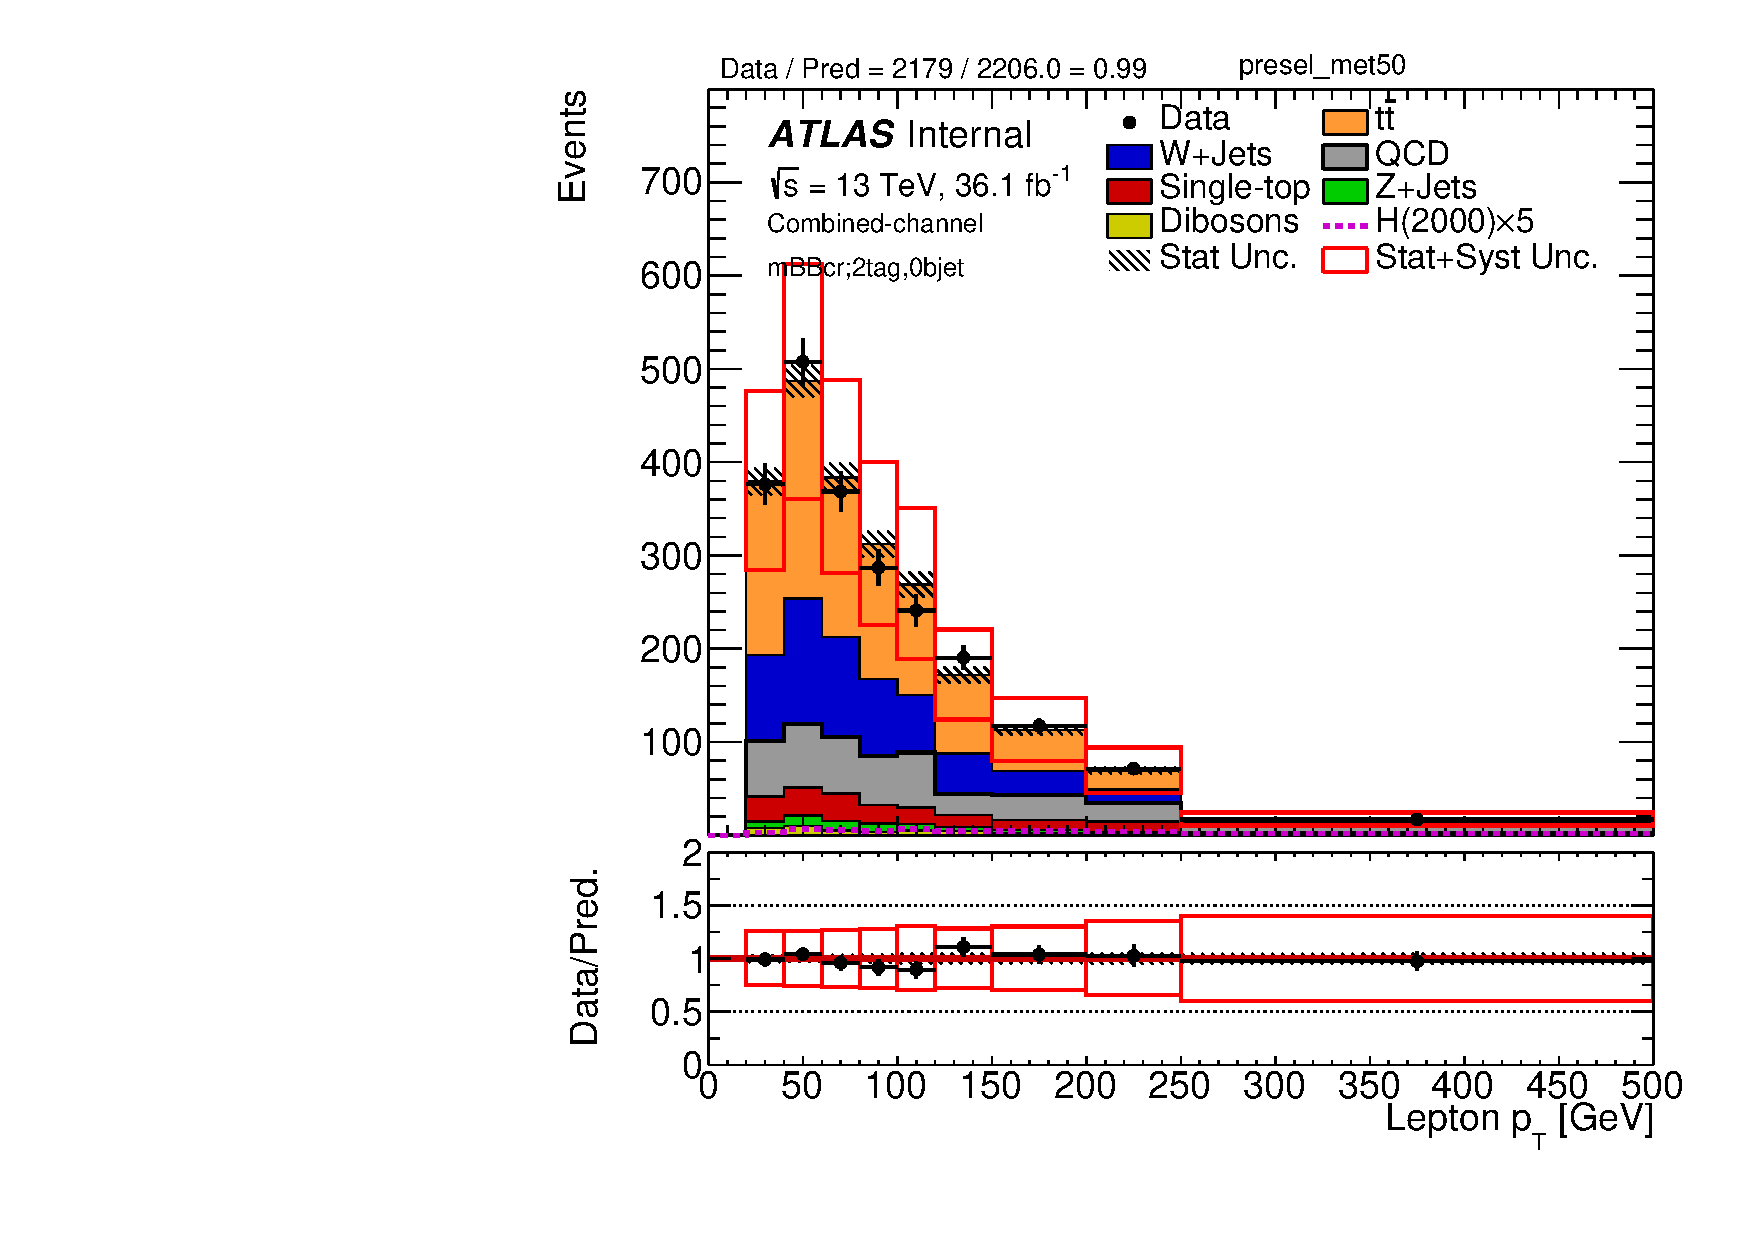
\includegraphics[width=0.49\textwidth]{./figures/boosted/PlotsInMbbCR/DataMC_2tag_0bjet_mbbcr_lepton_presel_met50_LepPt}
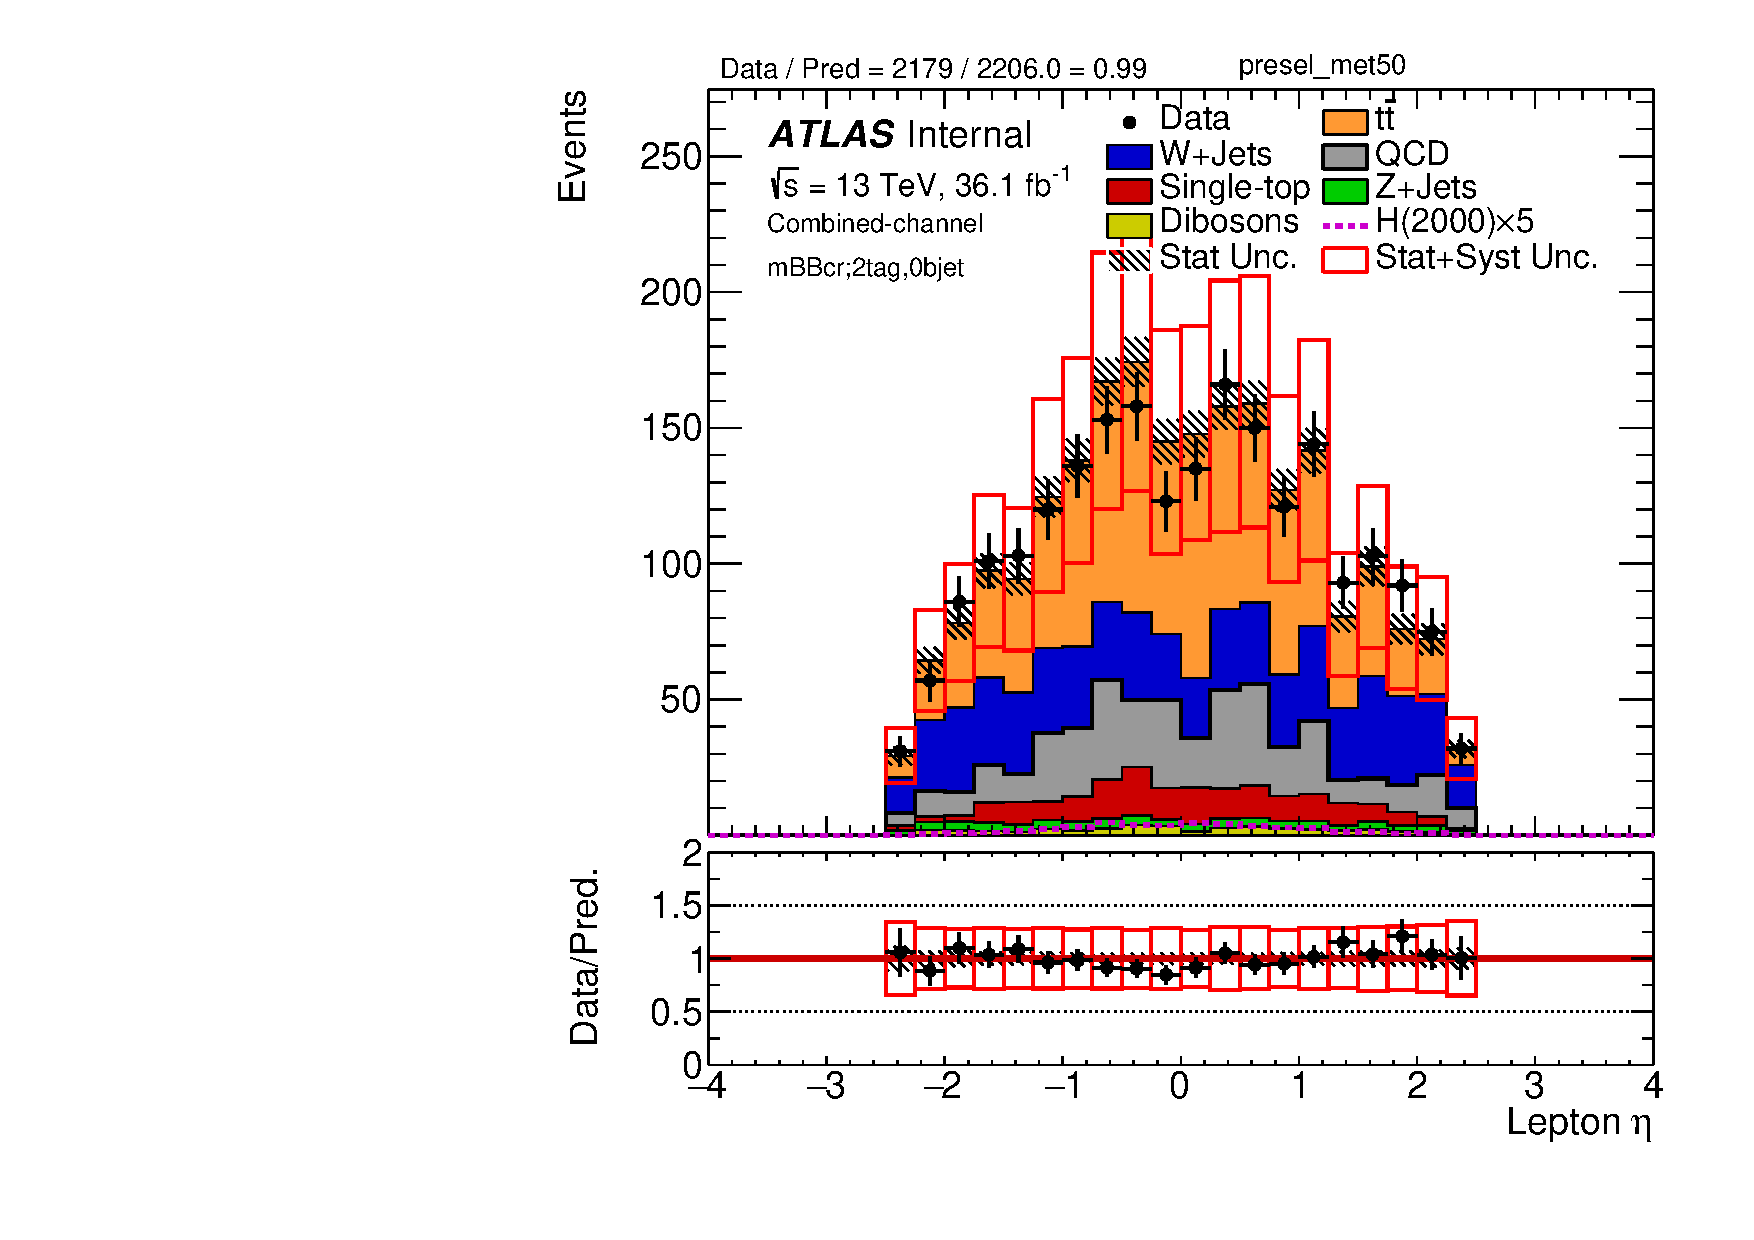
\includegraphics[width=0.49\textwidth]{./figures/boosted/PlotsInMbbCR/DataMC_2tag_0bjet_mbbcr_lepton_presel_met50_LepEta}\\
\par\medskip
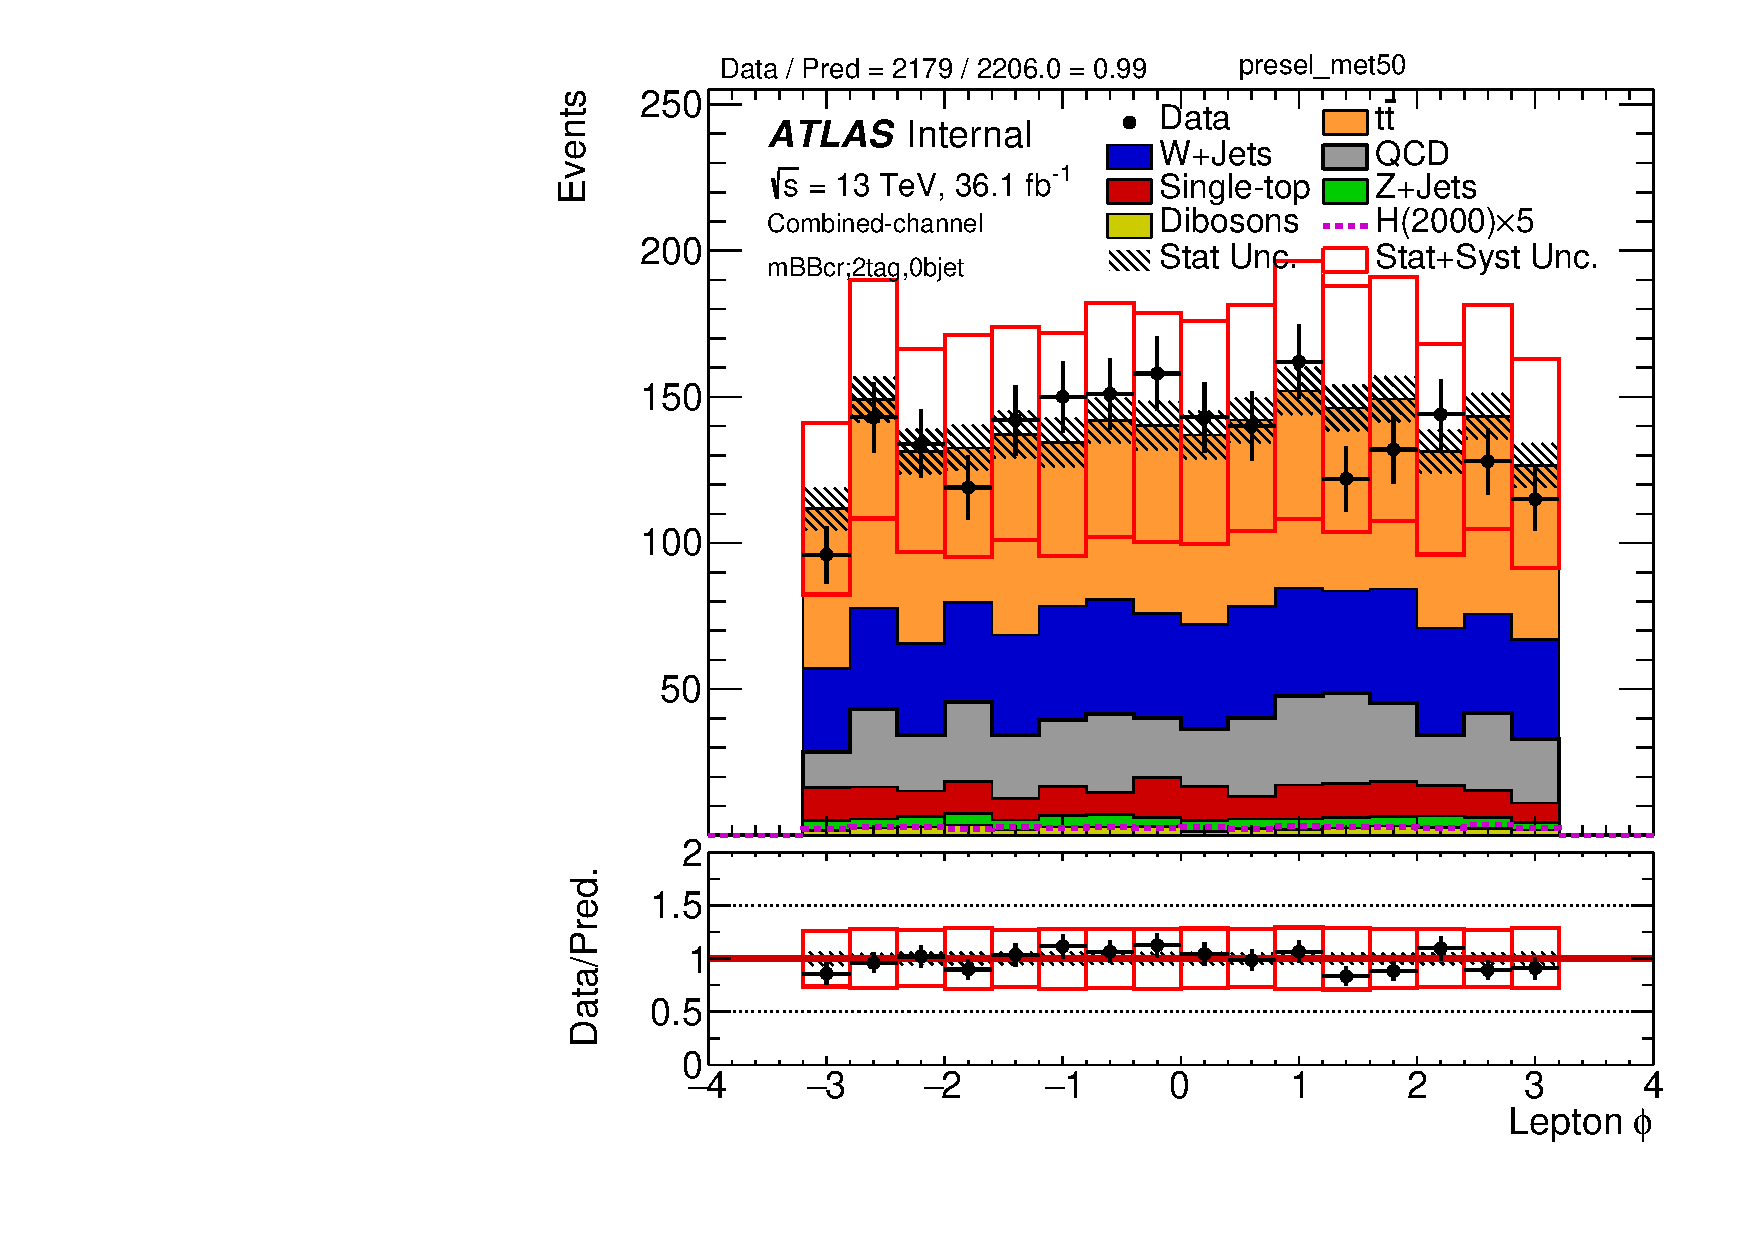
\includegraphics[width=0.49\textwidth]{./figures/boosted/PlotsInMbbCR/DataMC_2tag_0bjet_mbbcr_lepton_presel_met50_LepPhi}
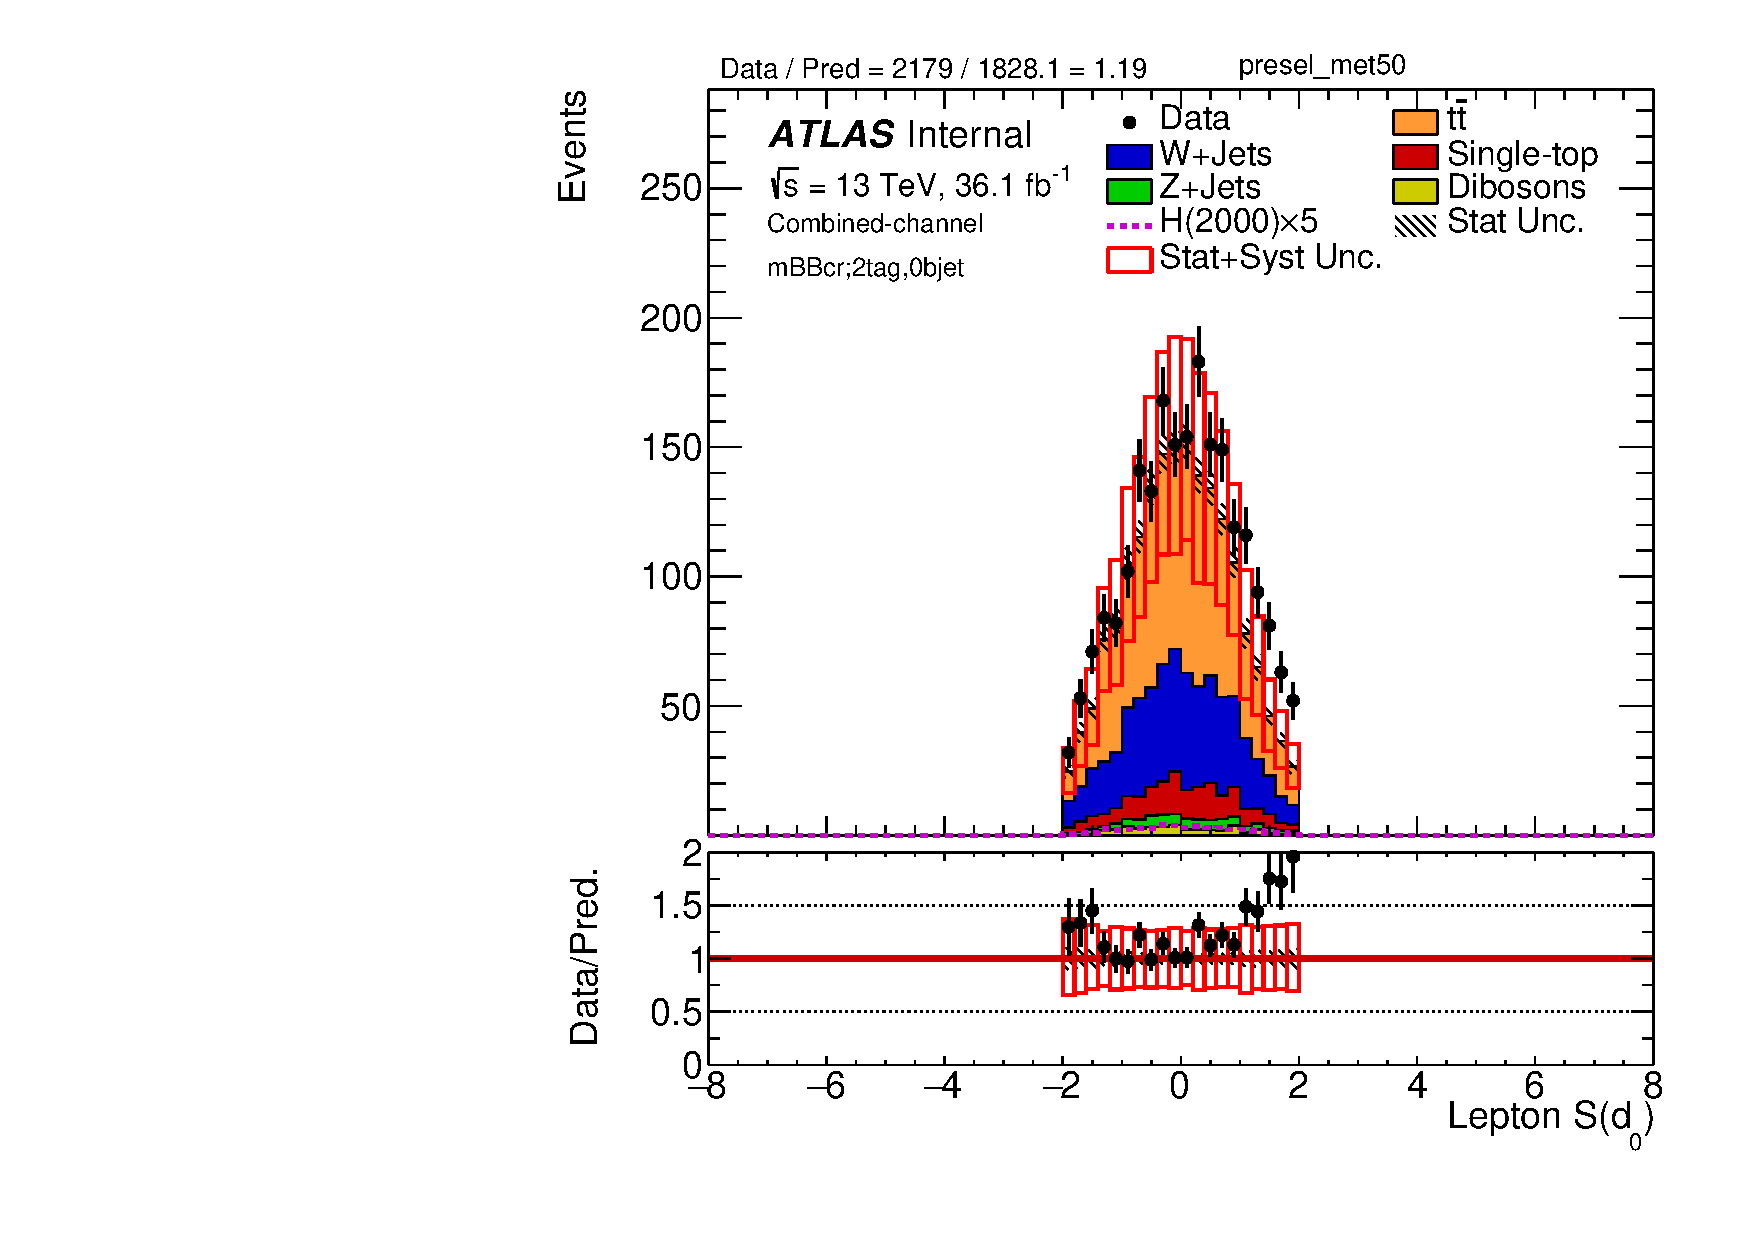
\includegraphics[width=0.49\textwidth]{./figures/boosted/PlotsInMbbCR/DataMC_2tag_0bjet_mbbcr_lepton_presel_met50_Lep_d0sigL}
\caption{Kinematic distributions of the selected lepton in the mBB control region (mBBcr).}
\label{fig:boosted_mbbcr_lepton}
\end{center}
\end{figure}
 \newpage
 
\begin{figure}[!h]
\begin{center}
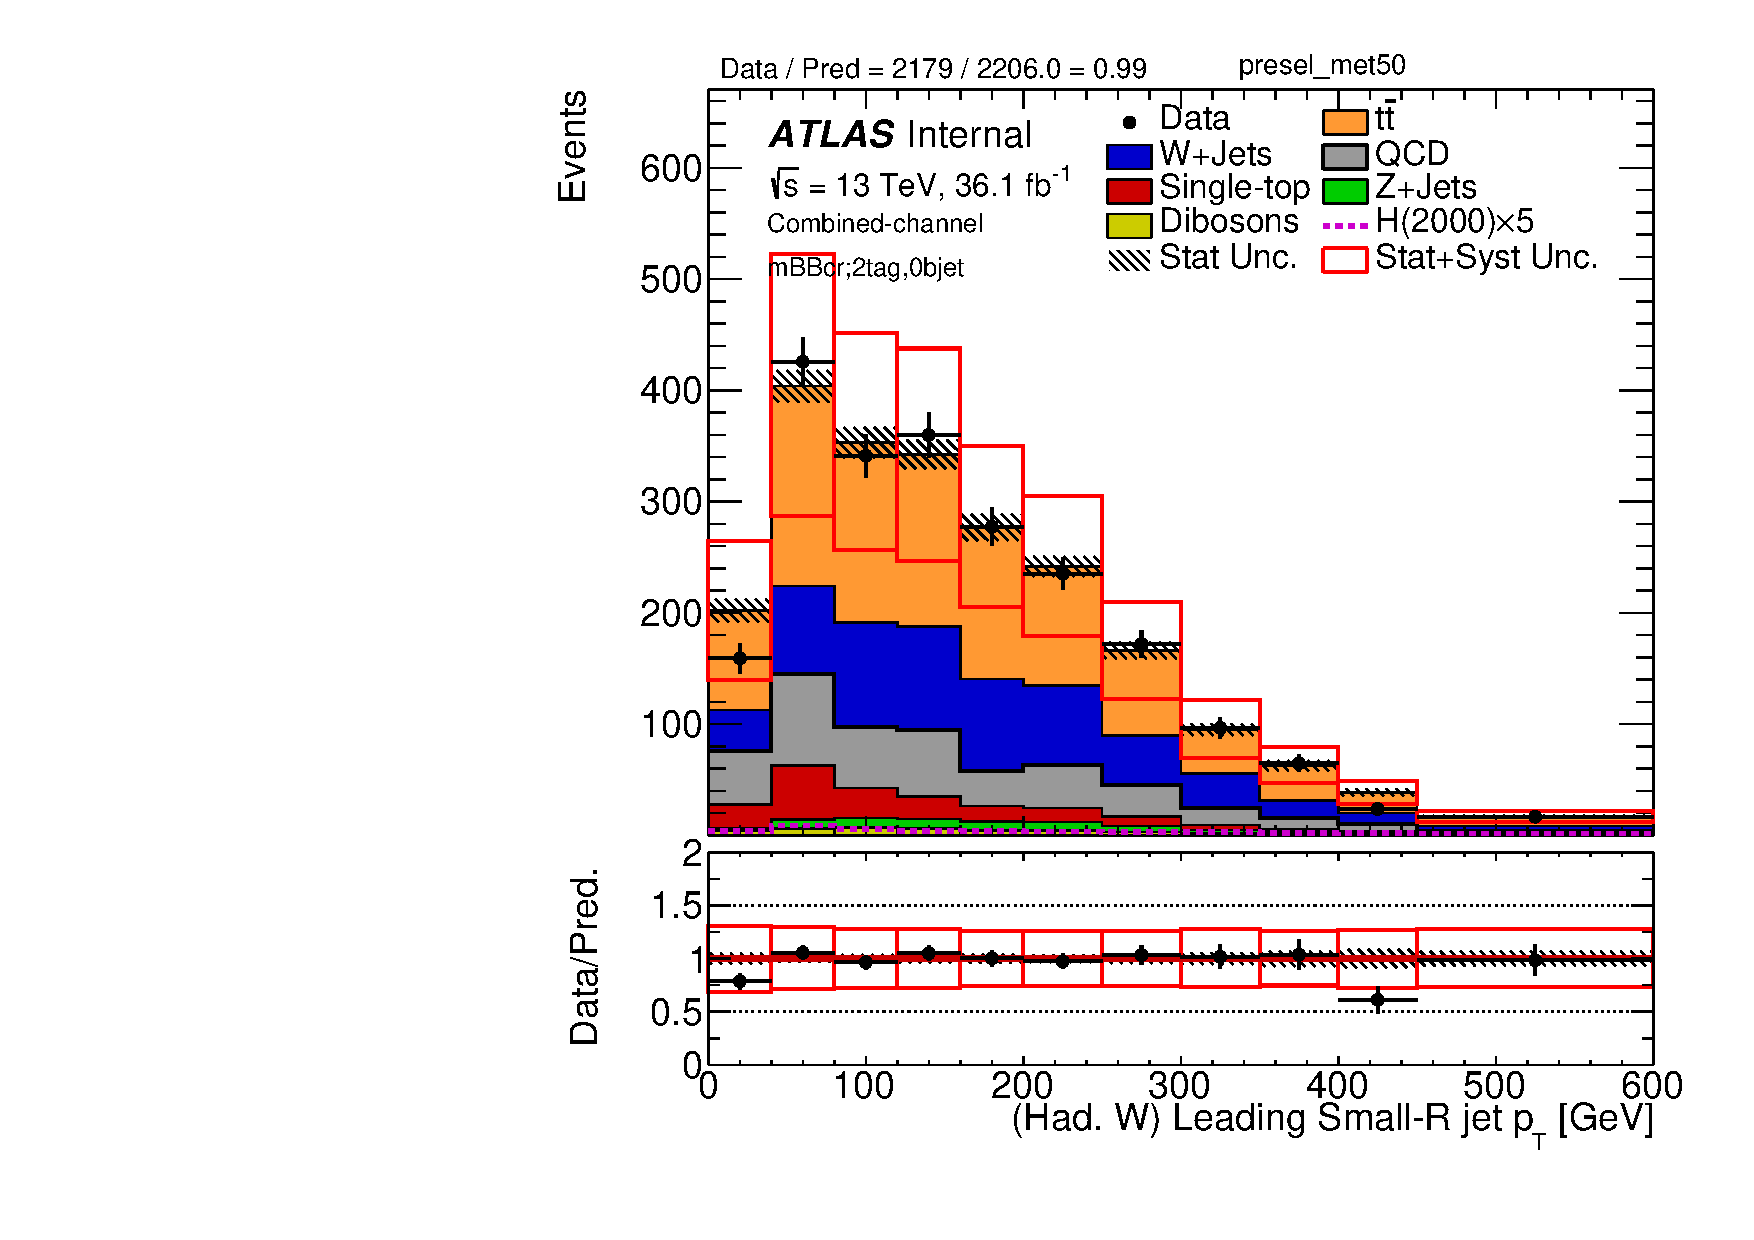
\includegraphics[width=0.49\textwidth]{./figures/boosted/PlotsInMbbCR/DataMC_2tag_0bjet_mbbcr_lepton_presel_met50_LightJet1Pt}
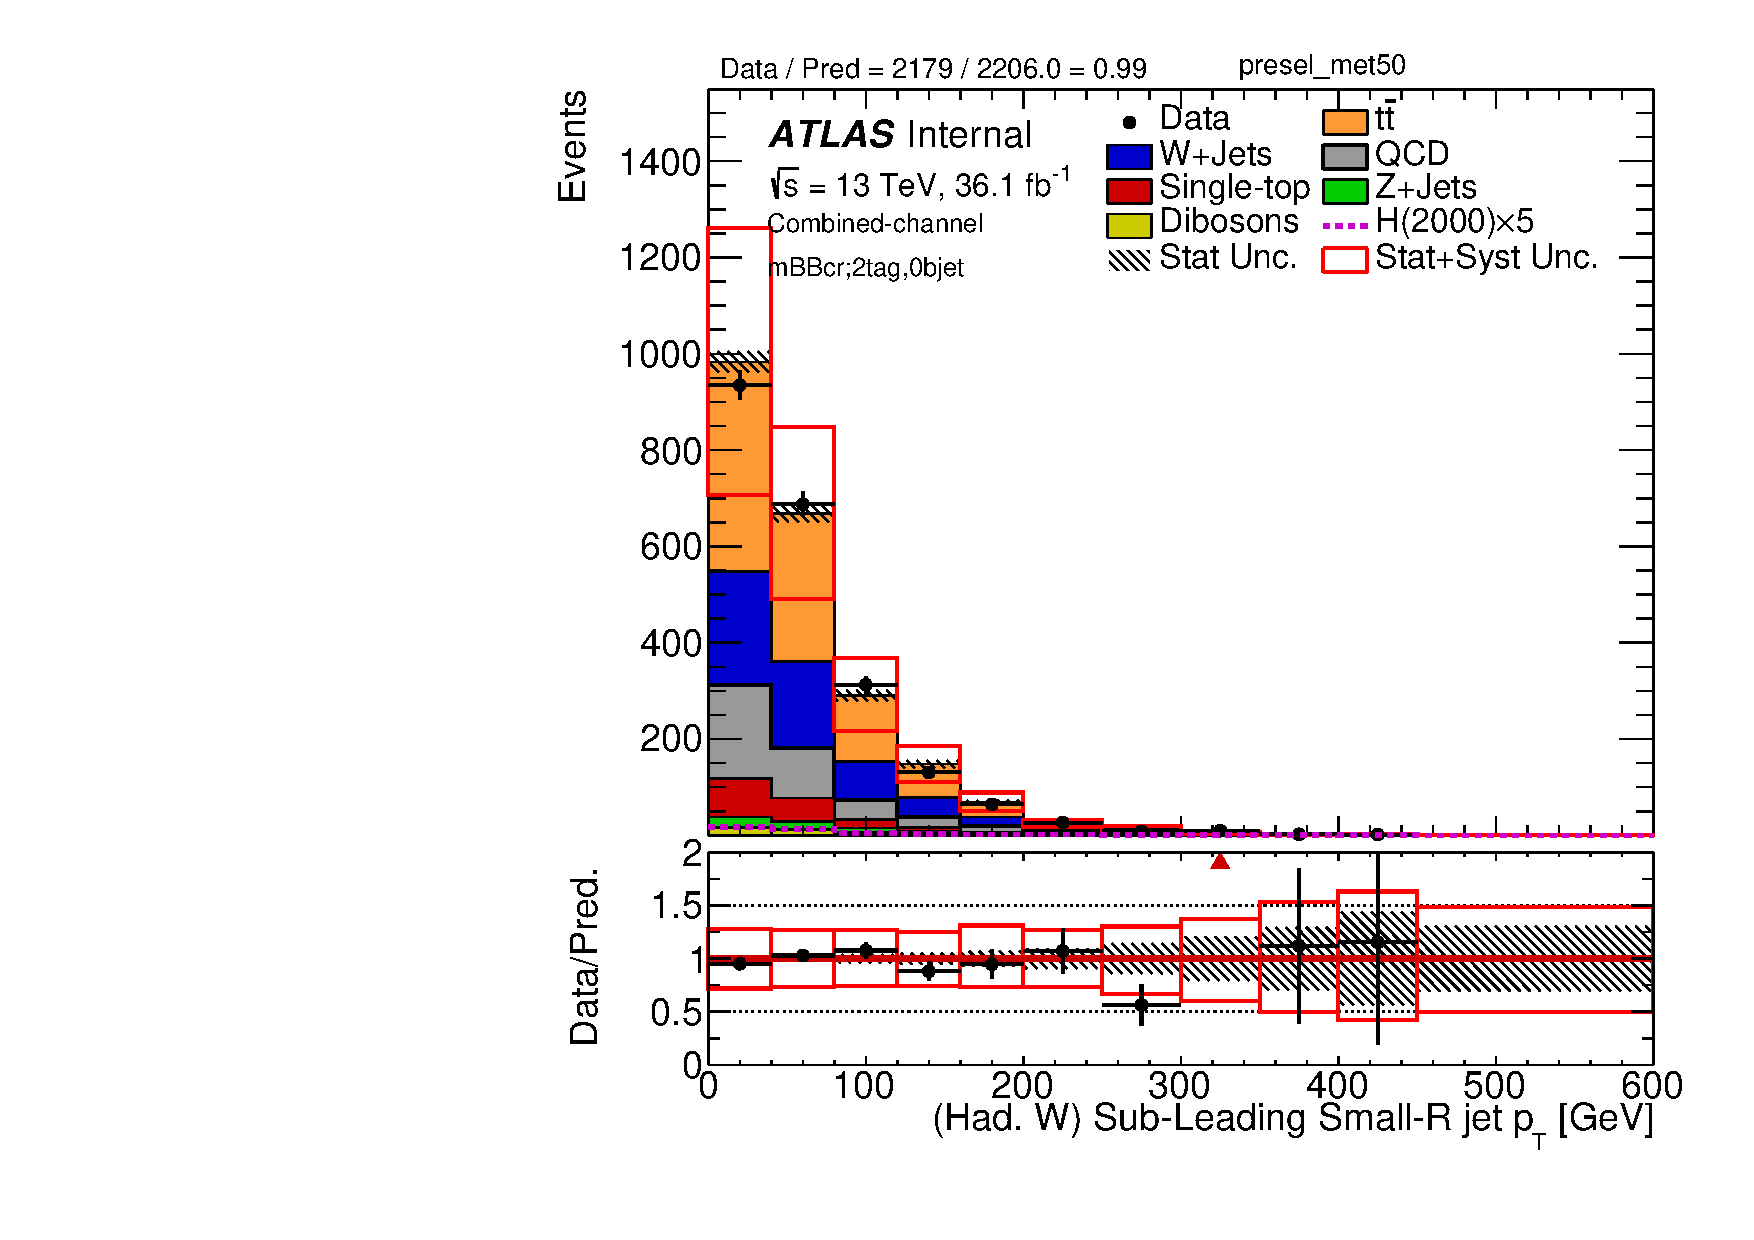
\includegraphics[width=0.49\textwidth]{./figures/boosted/PlotsInMbbCR/DataMC_2tag_0bjet_mbbcr_lepton_presel_met50_LightJet2Pt}\\
\par\medskip
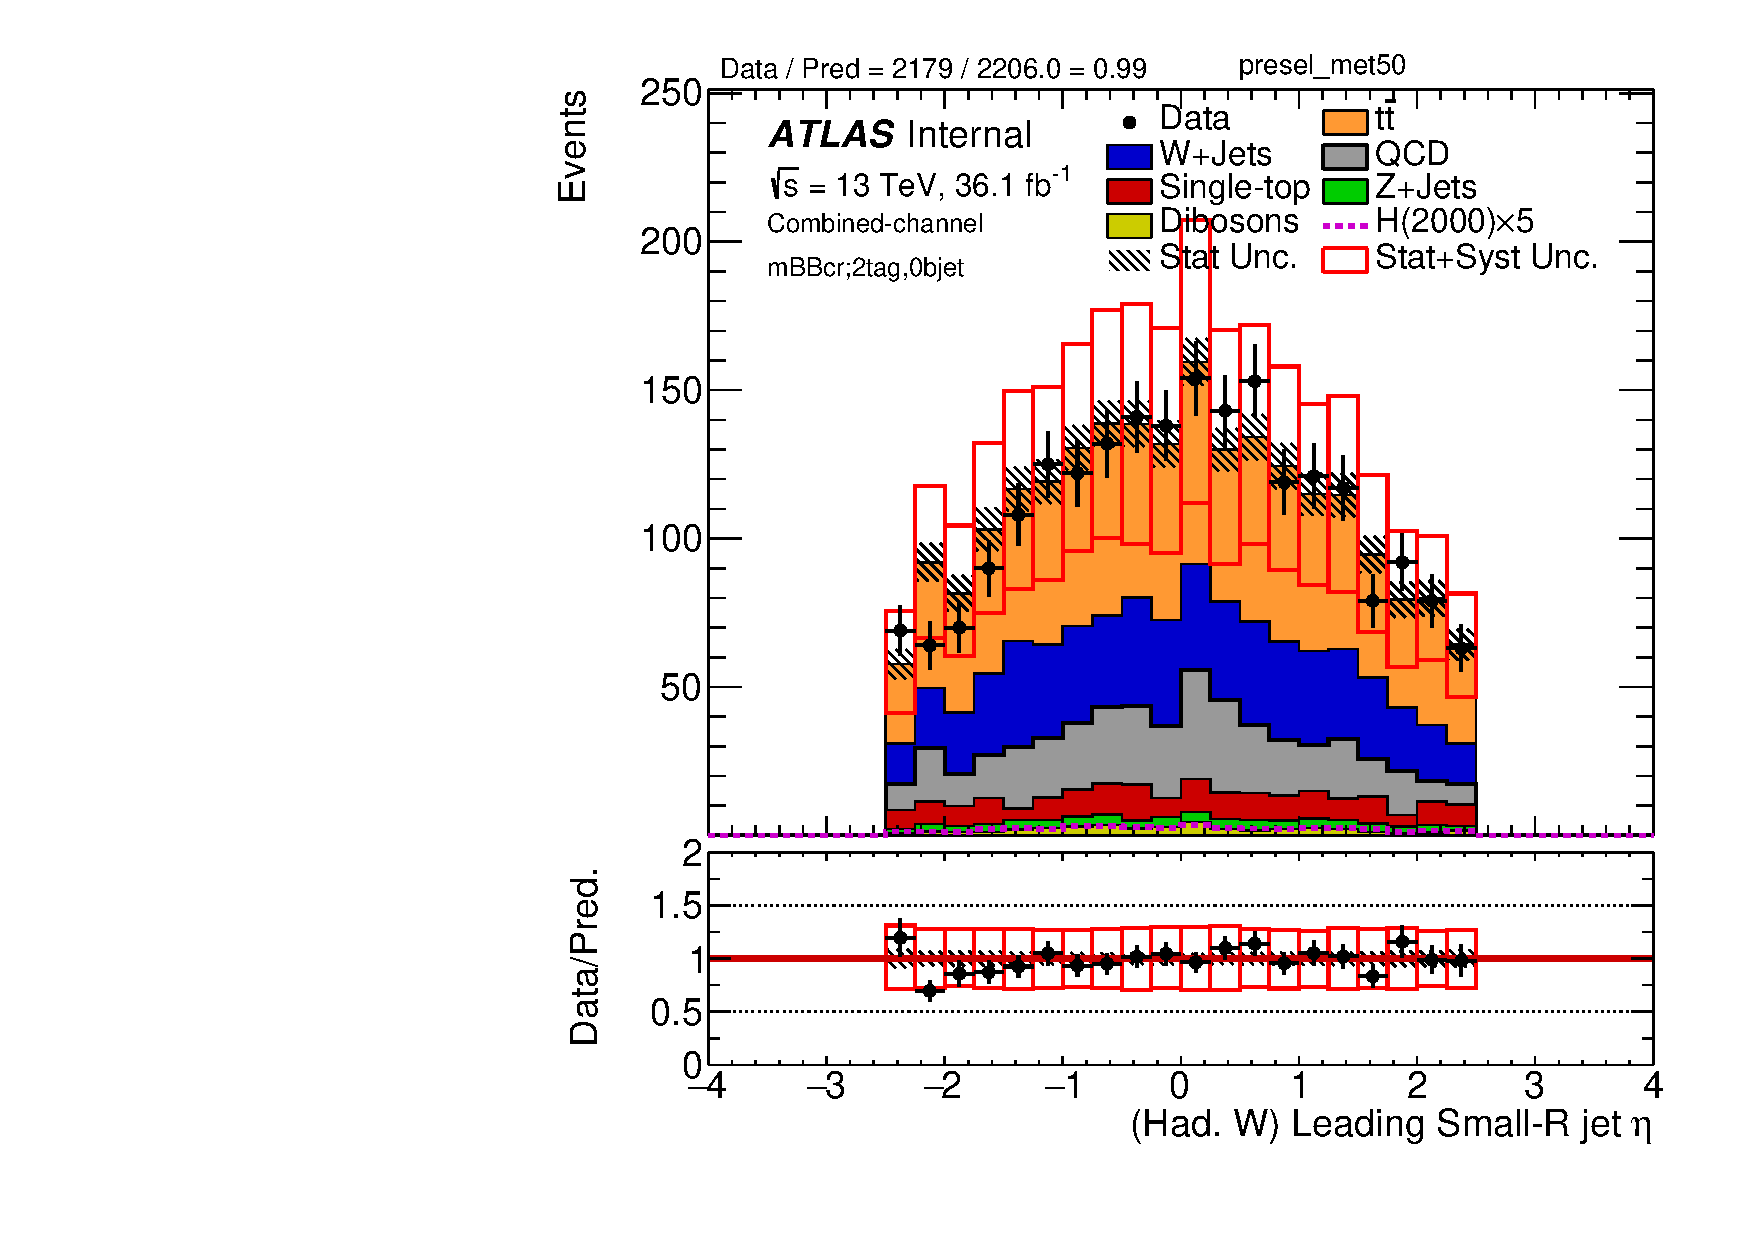
\includegraphics[width=0.49\textwidth]{./figures/boosted/PlotsInMbbCR/DataMC_2tag_0bjet_mbbcr_lepton_presel_met50_LightJet1Eta}
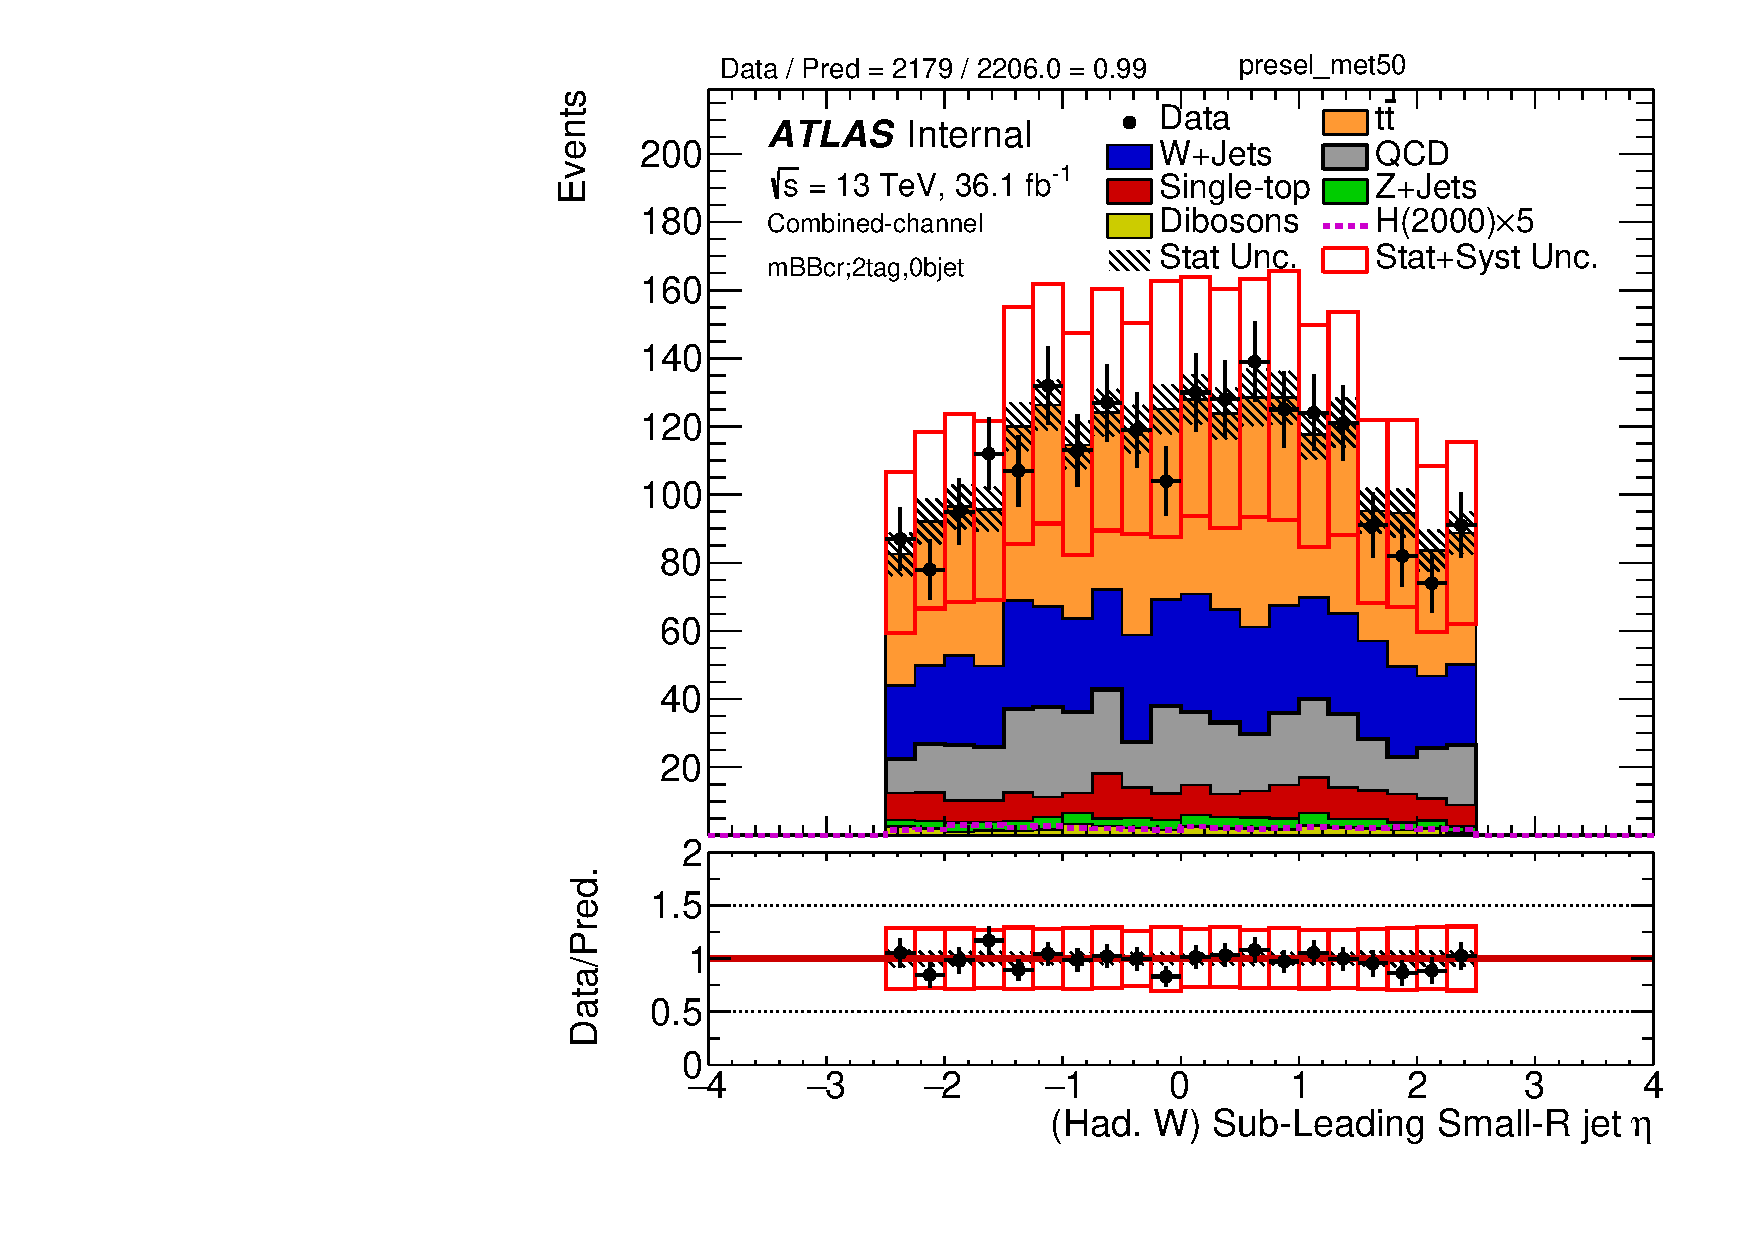
\includegraphics[width=0.49\textwidth]{./figures/boosted/PlotsInMbbCR/DataMC_2tag_0bjet_mbbcr_lepton_presel_met50_LightJet2Eta}\\
\par\medskip
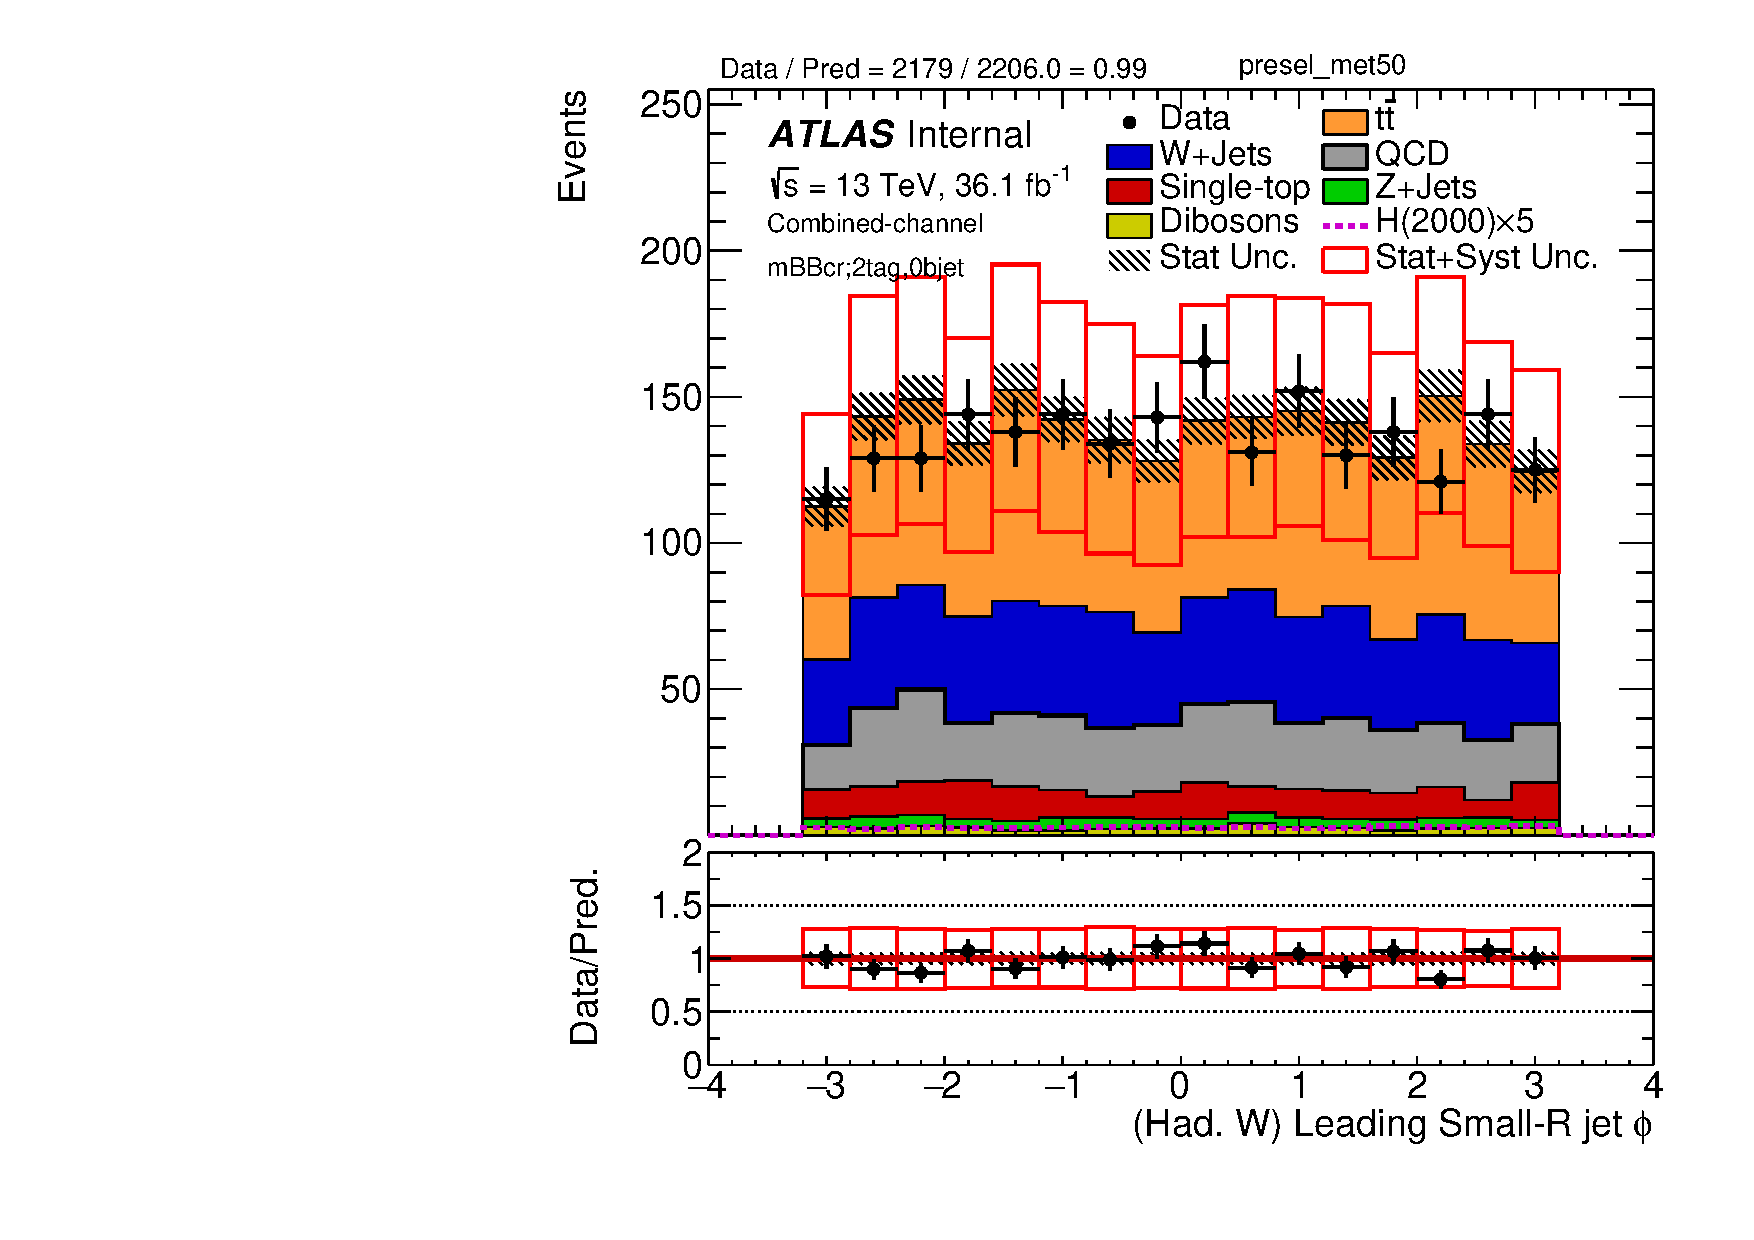
\includegraphics[width=0.49\textwidth]{./figures/boosted/PlotsInMbbCR/DataMC_2tag_0bjet_mbbcr_lepton_presel_met50_LightJet1Phi}
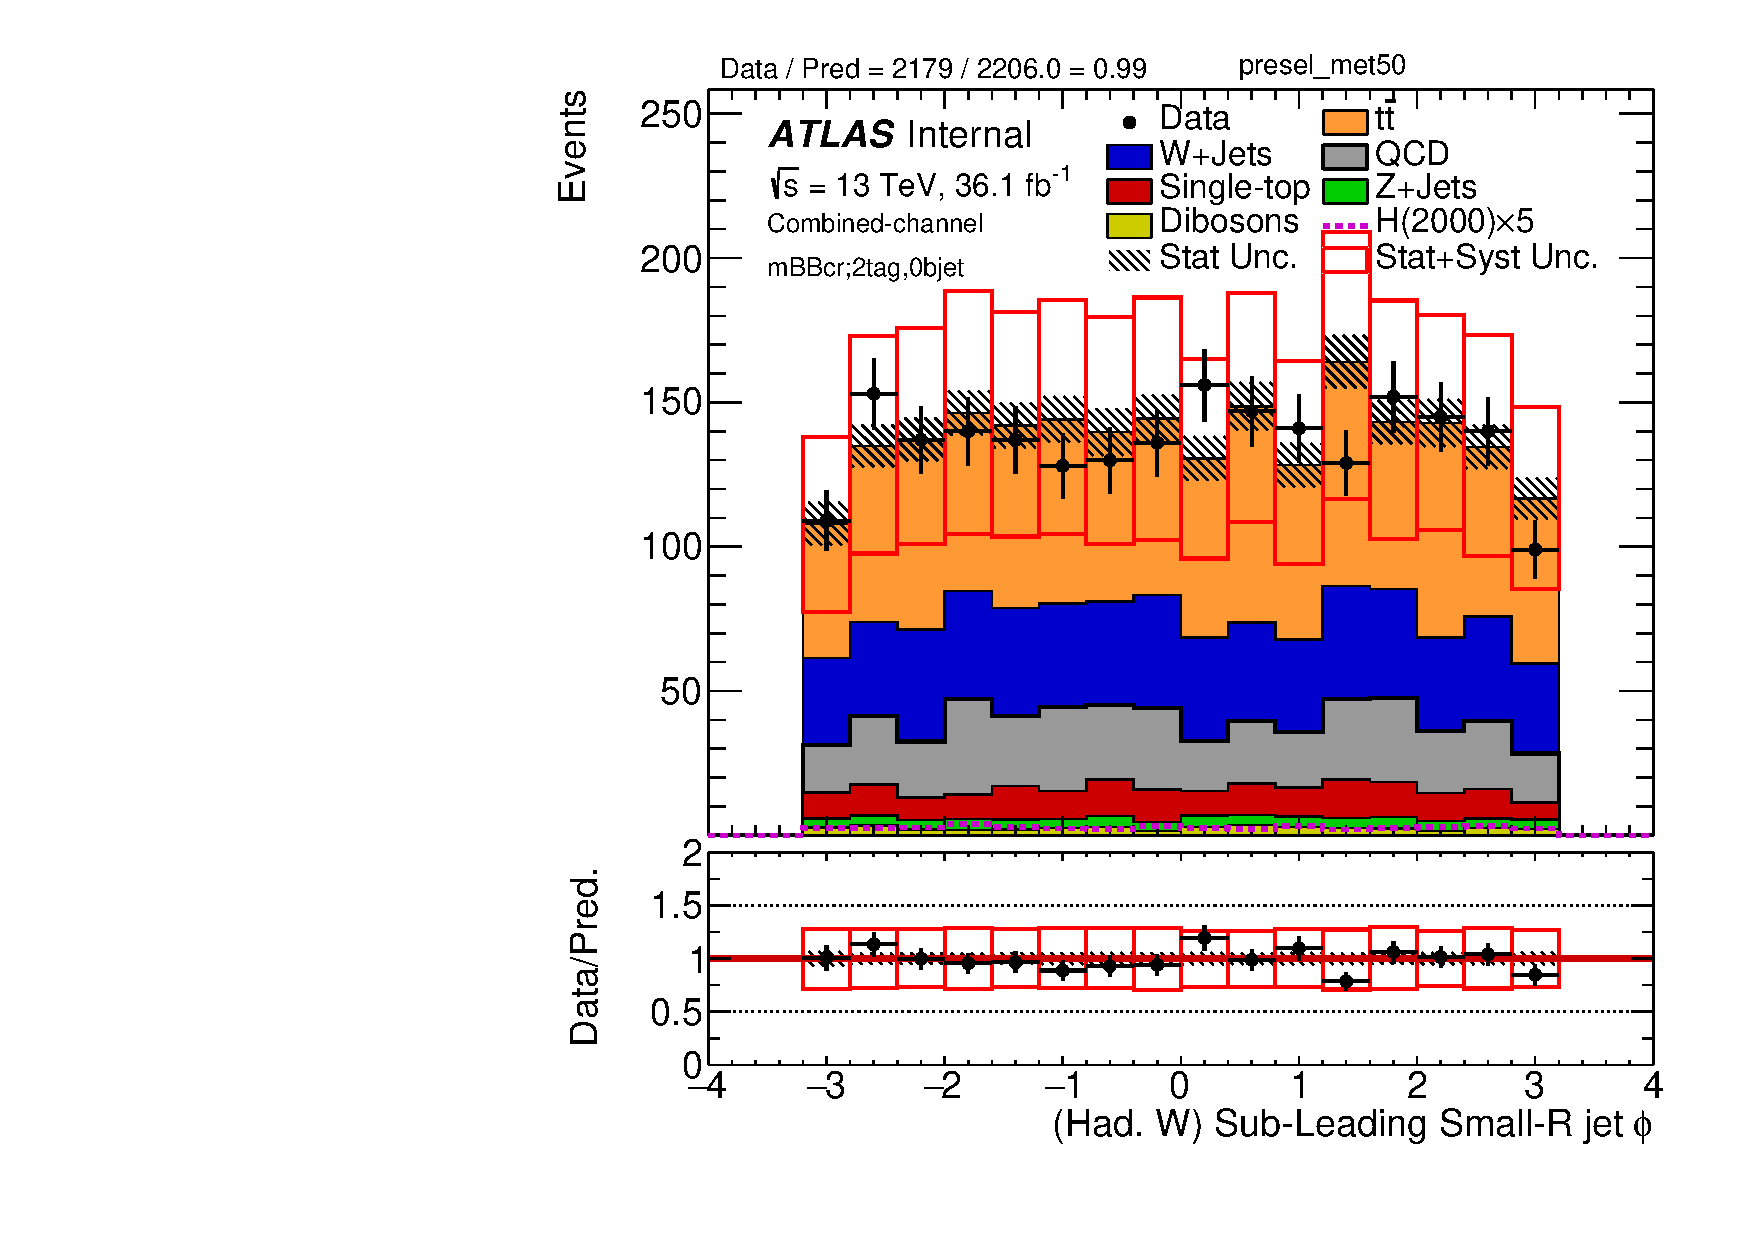
\includegraphics[width=0.49\textwidth]{./figures/boosted/PlotsInMbbCR/DataMC_2tag_0bjet_mbbcr_lepton_presel_met50_LightJet2Phi}\\
\caption{Kinematic distributions of the leading and sub-leading small-$R$ jets (of the reconstructed hadronic W)
in the mBB control region (mBBcr).}
\label{fig:boosted_mbbcr_whad_jets}
\end{center}
\end{figure}
 \newpage
\begin{figure}[!h]
\begin{center}
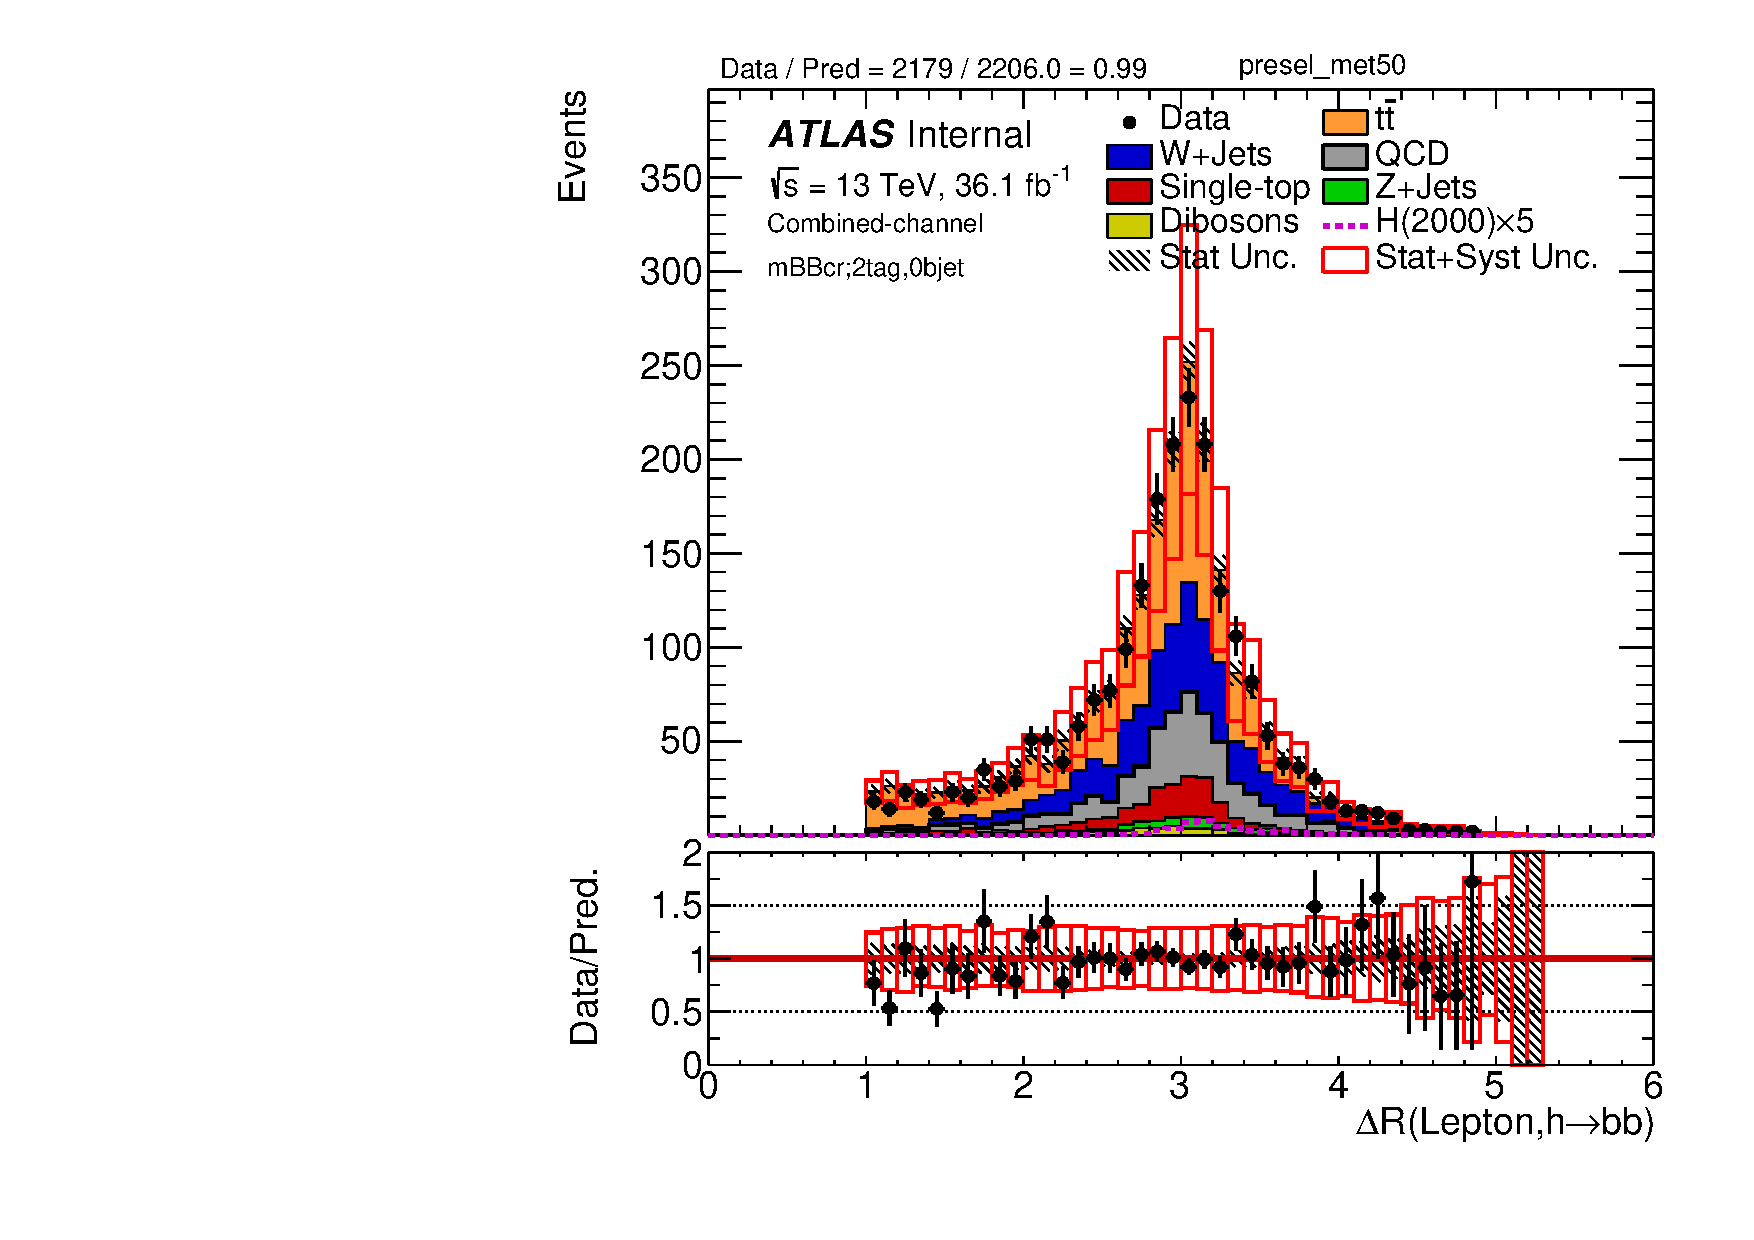
\includegraphics[width=0.49\textwidth]{./figures/boosted/PlotsInMbbCR/DataMC_2tag_0bjet_mbbcr_lepton_presel_met50_drHbbLep}
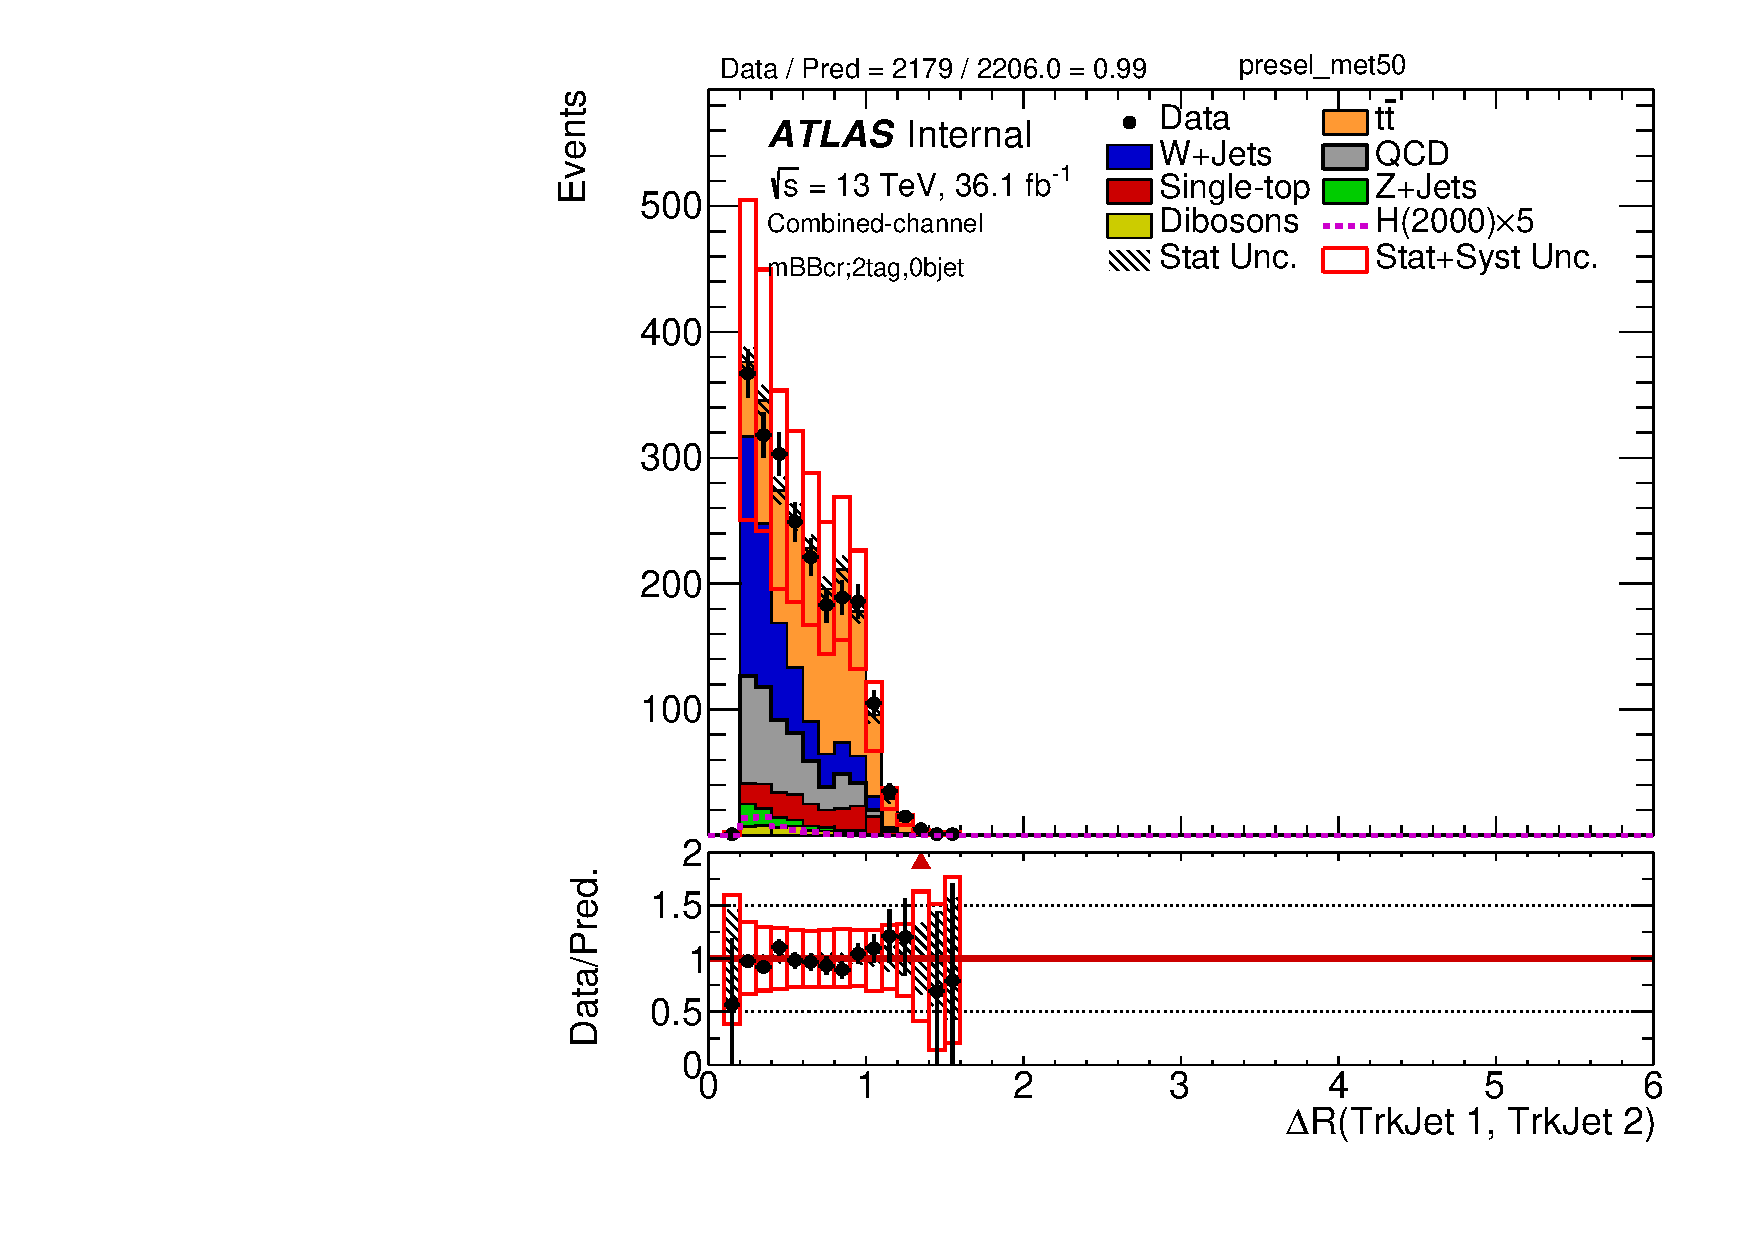
\includegraphics[width=0.49\textwidth]{./figures/boosted/PlotsInMbbCR/DataMC_2tag_0bjet_mbbcr_lepton_presel_met50_drbtrkjet1btrkjet2}\\
\caption{$\Delta R$ distribution between the selected lepton and the large-$R$ jet and $\Delta R$ distribution between the track-jets inside
the large-$R$ jet in the mBB control region (mBBcr).}
\label{fig:boosted_mbbcr_dr}
\end{center}
\end{figure}
 
\newpage
  
\subsection{Systematics}
\label{sec:boosted_systematics}
\subsubsection{Dectector modeling uncertainties}
\label{sec:boosted_syst_detector}
 
The experimental uncertainties considered in the analysis are listed in Table~\ref{tab:boosted_syst_detector}.
The uncertainties are applicable to signal and background processes that are modelled using MC simulation.
 
\begin{table}
\resizebox{\textwidth}{!}
{
\begin{tabular}{l|l}
 
\hline
Systematic uncertainty & Short description \\
\hline
\multicolumn{2}{c}{Event} \\
\hline
\texttt{ATLAS\_LUMI\_2015\_2016} & uncertainty on total integrated luminosity \\
\hline
\texttt{PRW\_DATASF} & pile-up reweighting uncertainty \\
\hline
\multicolumn{2}{c}{Electrons} \\
\hline
\texttt{EL\_EFF\_Trigger\_TOTAL\_1NPCOR\_PLUS\_UNCOR} &  trigger efficiency uncertainty \\
\texttt{EL\_EFF\_Reco\_TOTAL\_1NPCOR\_PLUS\_UNCOR}         &  reconstruction efficiency uncertainty \\
\texttt{EL\_EFF\_ID\_TOTAL\_1NPCOR\_PLUS\_UNCOR}         &  ID efficiency uncertainty \\
\texttt{EL\_EFF\_Iso\_TOTAL\_1NPCOR\_PLUS\_UNCOR}          &  isolation efficiency uncertainty \\
\texttt{EG\_SCALE\_ALL} &        energy scale uncertainty          \\        
\texttt{EG\_RESOLUTION\_ALL} &    energy resolution uncertainty    \\  
\hline
\multicolumn{2}{c}{Muons} \\
\hline
\texttt{MUON\_EFF\_TrigStatUncertainty} &  \multirow{2}{*}{trigger efficiency uncertainty} \\  
\texttt{MUON\_EFF\_TrigSystUncertainty} &  \\
\texttt{MUON\_EFF\_STAT} &  \multirow{2}{*}{reconstruction and ID efficiency uncertainty for muons}\\  
\texttt{MUON\_EFF\_SYS} &  \\
\texttt{MUON\_ISO\_STAT} &  \multirow{2}{*}{isolation efficiency uncertainty}\\  
\texttt{MUON\_ISO\_SYS} & \\            
\texttt{MUONS\_SCALE} &    energy scale uncertainty        \\                  
\texttt{MUONS\_ID} & energy resolution uncertainty from inner detector     \\                  
\texttt{MUONS\_MS} &  energy resolution uncertainty from muon system  \\
\hline
\multicolumn{2}{c}{Small-$R$ jets} \\
\hline
\texttt{JET\_SR1\_JET\_GroupedNP\_1} & \multirow{4}{*}{energy scale uncertainties strongly-reduced to 4 components.} \\
\texttt{JET\_SR1\_JET\_GroupedNP\_2} & \\
\texttt{JET\_SR1\_JET\_GroupedNP\_3} & \\
\texttt{JET\_SR1\_JET\_EtaIntercalibration\_NonClosure} &  \\
\texttt{JET\_JER\_SINGLE\_NP} & energy resolution uncertainty  \\
\texttt{JET\_JvtEfficiency} & JVT efficiency uncertainty   \\
% \texttt{FT\_EFF\_Eigen\_B} & \multirow{3}{*}{\parbox{11cm}{$b$-tagging efficiency uncertainties (``BTAG\_MEDIUM''): 3 components for $b$ jets, 4 for $c$ jets and 5 for light jets}} \\
% \texttt{FT\_EFF\_Eigen\_C} & \\
% \texttt{FT\_EFF\_Eigen\_L} & \\
% \texttt{FT\_EFF\_Eigen\_extrapolation} & $b$-tagging efficiency uncertainty on the extrapolation to high-\pt jets  \\
% \texttt{FT\_EFF\_Eigen\_extrapolation\_from\_charm} & $b$-tagging efficiency uncertainty on tau jets   \\
\hline
\multicolumn{2}{c}{Large-$R$ jets} \\
\hline
\texttt{FATJET\_Medium\_JET\_Comb\_Baseline\_Kin}  &  \multirow{4}{*}{energy scale uncertainties (\pT and mass scales are fully correlated)} \\
\texttt{FATJET\_Medium\_JET\_Comb\_modeling\_Kin} &   \\
\texttt{FATJET\_Medium\_JET\_Comb\_TotalStat\_Kin} &   \\
\texttt{FATJET\_Medium\_JET\_Comb\_Tracking\_Kin}  &  \\
\texttt{FATJET\_JER} &  energy resolution uncertainty    \\
\texttt{FATJET\_JMR} &  mass resolution uncertainty \\
\hline
\multicolumn{2}{c}{Track-jets and Small-R jets} \\
\hline    
\texttt{FT\_EFF\_Eigen\_B} & \multirow{3}{*}{\parbox{11cm}{$b$-tagging efficiency uncertainties (``BTAG\_MEDIUM''): 3 components for $b$ jets, 4 for $c$ jets and 5 for light jets}} \\
\texttt{FT\_EFF\_Eigen\_C} & \\
\texttt{FT\_EFF\_Eigen\_L} & \\
\texttt{FT\_EFF\_Eigen\_extrapolation} & $b$-tagging efficiency uncertainty on the extrapolation to high \pt jets  \\
\texttt{FT\_EFF\_Eigen\_extrapolation\_from\_charm} & $b$-tagging efficiency uncertainty on tau jets  \\
\hline
\multicolumn{2}{c}{\met} \\
\hline    
\texttt{MET\_SoftTrk\_ResoPara} & track-based soft term related longitudinal resolution uncertainty   \\
\texttt{MET\_SoftTrk\_ResoPerp} & track-based soft term related transverse resolution uncertainty   \\
\texttt{MET\_SoftTrk\_Scale}    & track-based soft term related longitudinal scale uncertainty   \\  
\hline
\end{tabular}
}
\caption{Summary of the (nuisance parameter) names and meanings of the detector modeling systematic uncertainties.}
\label{tab:boosted_syst_detector}
\end{table}
 
\paragraph{$|d_{0}^{\textrm{sig}}|$ cut efficiency modeling}
\label{sec:boosted_syst_d0cut}
 
In this analysis, the $|d_{0}^{\textrm{sig}}|$ cut value used for electrons and muons are not the recommended
value by CP groups. The recommended value for electrons is 5 while for muons it is 3. The modeling of the
$|d_{0}^{\textrm{sig}}|$ significance is assesed in a top-enriched control region. The event reconstruction and selection
criteria for the top-enriched control region are exactly the same as outlined in Section~\ref{sec:boosted_evtreco}
to~\ref{sec:boosted_regiondefs} with the exception that the $b$-tagging requirement on the event is different.
For this control region, each event is required to have either the leading or sub-leading track-jet to be $b$-tagged but not both track-jets to $b$-tagged.
The event is also required to have at least one $b$-tagged signal small-$R$ jets, which is in other words the $b$-jet veto is reversed. For the purposes
of studying the modeling the of the $|d_{0}^{\textrm{sig}}|$ distribution, no $|d_{0}^{\textrm{sig}}|$ requirement is applied on the reconstructed leptons.
 
\begin{figure}[!htbp]
\begin{center}
\includegraphics[width=0.49\textwidth]{./figures/boosted/Leptond0Plots/DataMC_1tag_1pbjet_Inc_elec_presel_met50_Lep_d0sigL} 
\includegraphics[width=0.49\textwidth]{./figures/boosted/Leptond0Plots/DataMC_1tag_1pbjet_Inc_muon_presel_met50_Lep_d0sigL} 
\caption{Electron and muon $d_{0}^{\textrm{sig}}$ distributions in the top control region without the large-$R$ jet mass cut.}
\label{fig:syst_d0_topcr}
\end{center}
\end{figure}
 
Figure~\ref{fig:syst_d0_topcr} shows the $|d_{0}^{\textrm{sig}}|$ distribution for the electron and the muon in the top-enriched control region. A clear bias
in Data can be observed and this is consistent with other studies throught ATLAS. In order to take into account the effect of the mismodeling of the $d_{0}^{\textrm{sig}}$
bias on the tight $d_{0}^{\textrm{sig}}$ cut used in this analysis, the efficiency of the $|d_{0}^{\textrm{sig}}|$ cut is evaluated and compared between Data and MC.
Table~\ref{tab:syst_d0_topcr_eff_datamc} shows the efficiency of the $|d_{0}^{\textrm{sig}}|$ cut in Data and MC and the ratio of effieciency between Data and MC in each
lepton channel. The relative difference between Data/MC ratio and unity is taken as the uncertainty on the $|d_{0}^{\textrm{sig}}|$ significance cut efficiency
and it is assigned for all processes with prompt leptons modelled by MC simulation. The nuisance parameter name associated to this uncertainty is \texttt{LEP\_d0\_CutEff}
 
\begin{table}[!htbp]
\begin{center}
\begin{tabular}{c|c|c}
&  Electron  & Muon  \\  
\hline
\multicolumn{3}{c}{$|d_{0}^{\textrm{sig}}| < 2.0$} \\
\hline
Data                &  0.884  & 0.897 \\
MC                  &  0.926  & 0.937 \\
\hline
Data/MC             &  0.955  & 0.957 \\
\hline
\hline
\multicolumn{3}{c}{$|d_{0}^{\textrm{sig}}| > 2.0$} \\
\hline
Data                &  0.115  & 0.104  \\
MC                  &  0.074  & 0.063  \\
\hline
Data/MC             &  1.572  & 1.640  \\
\end{tabular}
\end{center}
\caption[Efficiency of the $|d_{0}^{\textrm{sig}}|$ cut for electrons and muons in Data
and MC]{Efficiency of the $|d_{0}^{\textrm{sig}}|$ cut for electrons and muons in Data
and MC. The Data/MC ratio is also calculated and the difference between the ratio and unity
is taken as the systematic uncertainty on the $|d_{0}^{\textrm{sig}}|$ efficiency modeling
for events with leptons that pass ($< 2.0$) or fail ($> 2.0$) the $|d_{0}^{\textrm{sig}}|$ cut.}
\label{tab:syst_d0_topcr_eff_datamc}
\end{table}
 
\FloatBarrier
%---------------------------------------------------------------------------------------------------------------
 
\subsubsection{Background and Signal modeling Systematics}
\label{sec:boosted_syst_modeling}
 
%---------------------------------------------------------------------------------------------------------------
 
\paragraph{Methodology}
\label{sec:boosted_syst_modeling_method}
 
Uncertainties in the $m_{HH}$ distributions are assigned to the dominant backgrounds, $t\bar{t}$ and V+Jets and
single top by comparing the nominal MC samples to a number of alternative MC generators at the reconstruction
level. The comparisons are performed in with the same event selection in Section ~\ref{sec:Boosted}.
Each uncertainty contains two components, a shape systematic and a normalization systematic due to acceptance.
 
The shape systematic corresponds to a reweighting function derived by fitting a 1$^\text{st}$ order polynomial to the
ratio of $m_{HH}$ distribution of the variation sample over the nominal sample. The $m_{HH}$ distribution for the
the variation sample is normalized to the same number of events of the norminal sample.
 
% \begin{equation}
% \label{eq:MCShapeSystFormula}
% \frac{h^{var}_{i}}{h^{nom}_{i}}
% \end{equation}
 
% Where $h^{nom}_{i}$ ($h^{var}_{i}$) corresponds to the $i^{th}$ $m_{hh}$ bin of the nominal (variation) MC sample.
 
% Differences in the normalization of each fit region can also be tested using the MC-to-MC comparisons, and are incorporated into the fit as
% a nuisance parameter $\theta_{k}$ that controls the relative ratio of two coupled regions. A single nuisance paramter controls the relative ratio
% of each set of coupled fit regions denoted as $R = \frac{A}{B}$, where $A/B$ represent a pair of coupled analysis fit regions that satisfy the
% condition $A \neq B$. The sets of coupled regions are as follows: $A/B = [\{SR,CR\}(\text{1-lep only}), \, \{0-lep,1-lep\}, \, \{1-lep,2-lep\},
% \, \{SR,topemucr\}(\text{2-lep only}), \, \{Resolved,Boosted\}]$. Each nuisance parameter is constrained using a prior uncertainty ($\sigma_{w_{accept}}$)
% derived from the MC-to-MC comparisons, where a $\theta(\frac{A}{B})_{k} = \pm 1$ pull corresponds to a $1 \pm 1\sigma_{w_{accept}}$ scale factor on the
% physical process in the numerator region ($A$ in this case). The prior uncertainty is derived using the formula:
 
% \begin{equation}\label{eq:MCAcceptanceSystFormula}
%  \sigma_{w_{accept}} = \sqrt{ \sum^{M}_{i}  \Bigg(\frac{ { \Big|\frac{n^{var^{i}}_{A}}{n^{var^{i}}_{B}}  - \frac{n^{nom}_{A}}{n^{nom}_{B}}\Big| } }{ \frac{n^{nom}_{A}}{n^{nom}_{B}} }\Bigg)^{2} }
% \end{equation}
 
% Where $n$ correponds to the total event yield, $M$ represents the total number of MC comparisons made for each physical process (see subsections \ref{sec:boosted_syst_modeling_top} \& \ref{sec:boosted_syst_modeling_vjets}), and the subscripts A/B denote the two coupled fit regions. The superscripts \textit{nom} \& $var^{i}$ denote the nominal MC and $i^{th}$ variation samples. When multiple MC-to-MC comparisons are made ($M \geq 2$), then quadrature sum of the individual priors is taken. As outlined in section \ref{sec:StatAnalysis}, each nuisance parameter is modelled as a log-normal (or Gaussian) distribution with an associated width parameter (width of the underlying Gaussian $\sigma$); this Gaussian constraint is defined by the above acceptance variation factor.
 
 
 
%---------------------------------------------------------------------------------------------------------------
 
\paragraph{Top-quark processes ($t \bar{t}$ \& single top) }
\label{sec:boosted_syst_modeling_top}
 
Four alternative MC $t \bar{t}$ samples are used to assess 3 aspects of the MC modeling,
whilst five alternative MC samples are used to assess 4 aspects of the MC modeling for
single top quark pair production. The alternative samples considered are:
 
\begin{itemize}
\item \textbf{\POWHEG+Herwig++:} The ME \POWHEG \;generator uses the same setup as that used for the nominal \POWHEG+\PYTHIA6 configuration,
but the parton shower (PS) generator is swapped out for Herwig++ version 2.7.1 using the UE-EE-5 tune and CTEQ6L1 PDF set.
The purpose therefore of this comparison is to test the PS, hadronisation, underlying event (UE) and Multiple Parton Interation (MPI) models
whilst maintaining the same hard scattering model given by \POWHEG.
 
\item \textbf{aMC@NLO+Herwig++:} The ME generator is swapped out for aMC@NLO using the CT10 PDF set, interfaced with Herwig++
using the CTEQ6L1-UE-EE-5 tune and CTEQ6LI PDF set. This sample is compared to the previous \POWHEG+Herwig++ sample.
This fixes the PS generator component, but alters the hard scattering generator, making this variation sensitive to the hard scatter model.
 
\item \textbf{\POWHEG+\PYTHIA6 Radhi/RadLo:} Using the same setup as that used for the nominal \POWHEG+\PYTHIA6 sample,
the RadHi and RadLo samples correspond to either the enhancement (high) or reduction (low) of initial/final state radiation (IFSR).
The two samples are compared to the nominal sample setup, and so are sensitive to variations of IFSR models.
   \begin{itemize}
   \item RadHi: The renormalization ($\mu_{R}$) and factorisation scale ($\mu_{F}$) scales are decreased by a factor of 0.5,
   the \POWHEG \, \textsf{hdamp} parameter is doubled ($2 \times m_{top}$), and the high radiation PERUGIA2012 tune is used.
   \item RadLo: The renormalization ($\mu_{R}$) and factorisation scale ($\mu_{F}$) scales are increased by a factor of two,   the \POWHEG \, \textsf{hdamp} parameter is kept at $m_{top}$, and the low radiation PERUGIA2012 tune is used.
   \end{itemize}
 
\item \textbf{\POWHEG+\PYTHIA6 Diagram Subtraction:} For the production of a single top quark in association with a W-boson ($Wt$)
the interference with the $t\bar{t}$ production process at NLO in QCD is removed by subtracting the cross-section
associated with the $t\bar{t}$ double resonance amplitude terms, rather than subtracting the same terms from the
amplitude prior to the calculation (Diagram Removal).
\end{itemize}
 
Table~\ref{tab:boosted_unc_ttbar} shows the estimated uncertainty on the normalization of the $t\bar{t}$ background in the signal region
from the comparison of the nominal $t\bar{t}$ sample to the alternative samples. The largest uncertainty comes the RadLo variation,
which is about $\sim$8.4\% with similar level of uncertainties from alternative ME generator choice and alternative PS generator choice.
The normalization of $t\bar{t}$ background is assinged with a single nuisance parameter with the total uncertainty set as the prior uncertainty.
 
Shape comparisons of the $m_{HH}$ distribution between the nominal $t\bar{t}$ sample to the alternative samples were made and they are shown in
Figure~\ref{fig:boosted_unc_ttbar_shape_sr} and Figure~\ref{fig:boosted_unc_ttbar_shape_sr_b}. %Appendix~\ref{app:boosted_syst_ttbar} documents studies on the normalization and shape systematics for $t\bar{t}$ background.
 
\begin{table}[htbp!]
\begin{center}
\begin{tabular}{c|c}
Variation  &  Uncertainty (\%) \\
\hline
RadHi      &                 1.4 \\
RadLo      &                 8.4 \\
aMC@NLO    &                 7.1 \\
Herwig++   &                 7.8 \\
PDF        &                 1.9 \\
Scale      &                 5.0 \\
\hline
Total      &                13.5 \\
\end{tabular}
\end{center}
\caption[The normalization uncertainty for the $t\bar{t}$ background in the SR
from different sources]{The normalization uncertainty for the $t\bar{t}$ background in the signal region
from different sources. The total uncertainty is calculated as the sum of quadrature from all
the sources.}
\label{tab:boosted_unc_ttbar}
\end{table}
 
\begin{figure}[!htbp]
\begin{center}
\includegraphics[width=0.49\textwidth]{./figures/boosted/systematics/ttbar_alt_hhMass_SR_RadHi_rebin} 
\includegraphics[width=0.49\textwidth]{./figures/boosted/systematics/ttbar_fromfit_hhMass_SR_RadHi}  \\
\includegraphics[width=0.49\textwidth]{./figures/boosted/systematics/ttbar_alt_hhMass_SR_RadLo_rebin}
\includegraphics[width=0.49\textwidth]{./figures/boosted/systematics/ttbar_fromfit_hhMass_SR_RadLo}  \\
\caption[$m_{HH}$ distribution shape comparison between nominal $t\bar{t}$ sample and alternative samples]{$m_{HH}$ distribution shape comparison between nominal $t\bar{t}$ sample and alternative samples. Plot on the left is a direct
comparison between the nominal and alternative sample while on the right, the variation comes from the reweighted function applied to
the nominal $t\bar{t}$ sample. The linear fit in the ratio of the left plot is used as the reweighted function.}
\label{fig:boosted_unc_ttbar_shape_sr}
\end{center}
\end{figure}

\begin{figure}[!htbp]
\begin{center}
\includegraphics[width=0.49\textwidth]{./figures/boosted/systematics/ttbar_alt_hhMass_SR_Gen_rebin}  
\includegraphics[width=0.49\textwidth]{./figures/boosted/systematics/ttbar_fromfit_hhMass_SR_Gen}     \\
\includegraphics[width=0.49\textwidth]{./figures/boosted/systematics/ttbar_alt_hhMass_SR_Shower_rebin}
\includegraphics[width=0.49\textwidth]{./figures/boosted/systematics/ttbar_fromfit_hhMass_SR_Shower}   \\
\caption[$m_{HH}$ distribution shape comparison between nominal $t\bar{t}$ sample and alternative samples]{$m_{HH}$ distribution shape comparison between nominal $t\bar{t}$ sample and alternative samples. Plot on the left is a direct
comparison between the nominal and alternative sample while on the right, the variation comes from the reweighted function applied to
the nominal $t\bar{t}$ sample. The linear fit in the ratio of the left plot is used as the reweighted function.}
\label{fig:boosted_unc_ttbar_shape_sr_b}
\end{center}
\end{figure}
 
For the single-top background, only the uncertainties on the modeling of the Wt production process are considered since it is the dominant single-top process in the
signal region. Table~\ref{tab:boosted_unc_singletopwt} shows the estimated uncertainty on the normalization of the single-top background. The biggest uncertainties comes from
the PS generator choice and comparisons to the DS sample. The total uncertainty is abnormally large, which is larger than 100\%.
 
\begin{table}[htbp!]
\begin{center}
\begin{tabular}{c|c}
Variation   &  Uncertainty (\%) \\
\hline
RadHi       &               15.1 \\
RadLo       &               19.0 \\
Herwig++    &               33.5 \\
DR          &               72.5 \\
aMC@NLO     &               25.4 \\
\hline
Total      &                85.9 \\
\end{tabular}
\end{center}
\caption[The normalization uncertainty for the $t\bar{t}$ background in the SR
from different sources]{The normalization uncertainty for the $t\bar{t}$ background in the signal region
from different sources. The total uncertainty is calculated as the sum of quadrature from all
the sources.}
\label{tab:boosted_unc_singletopwt}
\end{table}
 
\FloatBarrier
 
%---------------------------------------------------------------------------------------------------------------
 
\paragraph{V+Jets processes}
\label{sec:boosted_syst_modeling_vjets}
 
The nominal V+Jets prediction, uses the ME+PS generator \SHERPA 2.2.1 interfaced with the NNPDF 3.0 NNLO PDF set.
This default configuration provides a prediction for vector boson production plus associated jets at NLO accuracy
at the ME level for up to 2 extra partons, and LO accuracy for 3 and 4 extra partons in QCD.
The merging of additional parton multiplicities arising from the internal \SHERPA PS, is regulated by the
MEPS@NLO merging technique.
 
The alternative samples used to assess the modeling uncertainties are:
 
\begin{itemize}
\item \textbf{MadGraph5+\PYTHIA8.186 :} The LO ME generator MadGraph5 using the NNPDF3.0(2.3) NLO(LO) PDF set interfaced
with \PYTHIA8 version 8.186 using the A14 tune, offers a LO+NLL accurate prediction for vector boson production in association
with jets for up to four extra partons from the ME and 4+ parton from \PYTHIA8 at NLL accuracy. The comparison between the nominal  
\SHERPA 2.2.1 sample with this sample convolves the ME and PS model variation. Due to the unavailability of this sample at
reconstruction level, the comparison is made at (particle) truth level.
 
\item \textbf{\SHERPA 2.2.1 scale variations:} Configured in the same manner as the nominal V+Jets sample,
the renormalization $\mu_{R}$ and resummation $\mu_{F}$ scales are varied up/down by a factor of two.
 
\item \textbf{\SHERPA 2.2.1 PDF variations:} Configured in the same manner as the nominal V+Jets sample. The
100 NNPDF3.0NNLO replicas variations are available. The central values of two alternative PDF sets, MMHT2014NNLO 68\% CL and CT14NNLO
are also available.
 
\item \textbf{\SHERPA 2.2.1 $\alpha_{s}(PDF)$ variations:} Configured in the same manner as the nominal V+Jets sample,
the $\alpha_{s}$ value used by the nominal NNPDF 3.0 NNLO PDF is varied up and down according to a variation of
the $\mu_{R}$ scale by a factor of two.
\end{itemize}
 
Table~\ref{tab:boosted_unc_wjets} shows the estimated uncertainty on the normalization of the W+jets background in the signal region
from the comparison of the nominal W+jets sample to the alternative samples.  The largest uncertainty comes from the renormalization
and resummation scale, which is about $\sim$42\% and dominates the total uncertainty on W+jets background. The normalization of W+jets
background is assinged with a single nuisance parameter with the total uncertainty set as the prior uncertainty.
 
Shape comparisons of the $m_{HH}$ distribution between the nominal W+jets sample to the alternative samples were made and only one
variation was found to have noticeable difference: the scale variation of $\mu_{R}$=0.5, $\mu_{F}$=0.5 as in Figure~\ref{fig:boosted_unc_wjets_sr_scale_fit}.
%Appendix~\ref{app:boosted_syst_wjets} documents studies on the normalization and shape systematics for W+jets background.
 
\begin{table}[htbp!]
\begin{center}
\begin{tabular}{c|c}
Variation  &  Uncertainty (\%) \\
\hline
Scale                 &   41.9  \\
$\alpha_{S}$(PDF)     &   8.4   \\
PDF alternative set   &   1.6   \\
NNPDF replicas        &   5.6   \\
Madgraph+Pythia8      &   11.0   \\
\hline
Total                 &   44.5  \\
\end{tabular}
\end{center}
\caption[The normalization uncertainty for the W+Jets background in the SR
from different sources]{The normalization uncertainty for the W+jets background in the signal region
from different sources. The total uncertainty is calculated as the sum of quadrature from all
the sources.}
\label{tab:boosted_unc_wjets}
\end{table}
 
\begin{figure}[!htbp]
\begin{center}
\includegraphics[width=0.49\textwidth]{./figures/boosted/systematics/wjets_alt_hhMass_SR_syst_SCALE_MUR0p5_MUF0p5_PDF261000}
\includegraphics[width=0.49\textwidth]{./figures/boosted/systematics/wjets_fromfit_hhMass_SR_SCALE_MUR0p5_MUF0p5_PDF261000} \\
\caption[$m_{HH}$ distribution shape comparison between nominal W+jets sample and scale variation ($\mu_{R}$=0.5, $\mu_{F}$=0.5) sample]{$m_{HH}$ distribution shape comparison between nominal W+jets sample and scale variation ($\mu_{R}$=0.5, $\mu_{F}$=0.5) sample. Plot on the left is a direct
comparison between the nominal and variation sample while on the right, the variation comes from the reweighted function applied to the nominal W+jets sample. The linear fit
in the ratio of the left plot is used as the reweighted function.}
\label{fig:boosted_unc_wjets_sr_scale_fit}
\end{center}
\end{figure}
 
Table~\ref{tab:boosted_unc_zjets} shows the estimated uncertainty on the normalization of the Z+jets background in the signal region
from the comparison of the nominal Z+jets sample to the alternative samples. The largest uncertainty comes from the renormalization
and resummation scale, which is about $\sim$48\% and dominates the total uncertainty on Z+jets background. The normalization of Z+jets
background is assinged with a single nuisance parameter with the total uncertainty set as the prior uncertainty. The uncertainty on the
$m_{HH}$ shape is found to be negligible and therefore ignored. %Appendix~\ref{app:boosted_syst_zjets} documents studies on the normalization and shape systematics for Z+jets background.
 
\begin{table}[htbp!]
\begin{center}
\begin{tabular}{c|c}
Variation  &  Uncertainty (\%) \\
\hline
Scale               &   48.3  \\
$\alpha_{S}$(PDF)   &   1.6   \\
PDF alternative set &   2.7   \\
NNPDF replicas      &   1.4   \\
\hline
Total               &   48.4  \\
\end{tabular}
\end{center}
\caption[The normalization uncertainty for the Z+Jets background in the SR
from different sources]{The normalization uncertainty for the Z+jets background in the signal region
from different sources. The total uncertainty is calculated as the sum of quadrature from all
the sources.}
\label{tab:boosted_unc_zjets}
\end{table}
 
\FloatBarrier
%---------------------------------------------------------------------------------------------------------------
\paragraph{Diboson processes}
\label{sec:boosted_syst_modeling_diboson}
The systematic uncertainty on the normalization of the Diboson background is assigned to be 40\%. This uncertainty
is taken from the resolved analysis. As the background is small, the uncertainty is considered to be conservative.
 
%---------------------------------------------------------------------------------------------------------------
\paragraph{Production}
\label{sec:boosted_syst_modeling_signal}
Systematic uncertainties on the acceptance of signal processes are computed by generating alternative variation signal samples
and then compare their acceptance with respect to the nominal signal samples. The difference sources of uncertainty considered are:
 
\begin{itemize}
\item \textbf{Scale variations:} Configured in the same manner as the nominal signal samples but
the renormalization and resummation scales are varied up/down by a factor of two.
 
% \item \textbf{PDF:}
 
\item \textbf{Parton shower choice:} Configured in the same manner as the nominal signal samples but
with Pythia 8 chosen as the shower generator instead of Herwig++.
\end{itemize}
 
Table~\ref{tab:boosted_unc_signal} lists the systematic uncertainties for four different scalar signal sample
mass points.
 
\begin{table}[htbp!]
\begin{center}
\begin{tabular}{c|c|c|c|c|c}
Variation    &  Xhh1000  &  Xhh1500 & Xhh2000 & Xhh2500 & Xhh3000   \\
\hline
Scale        &    0.2    &    0.2   &  0.4    &  0.4   &  0.4  \\
PDF          &    0.4    &    0.2   &  0.4    &  0.2   &  0.1  \\
Shower       &    0.4    &    0.8   &  1.6    &  3.4   &  4.1  \\
\end{tabular}
\end{center}
\caption{Theoretical uncertainties (in percentage) on the acceptance of several signal mass points.}
\label{tab:boosted_unc_signal}
 
 
\end{table}
%---------------------------------------------------------------------------------------------------------------
\subsubsection{QCD multijet modeling}
\label{sec:boosted_syst_modeling_multijet}
 
Systematic uncertainties related to the modeling of the multijet background were discussed in Section~\ref{sec:boosted_bkgd_qcdmultijet_yield_unc}
for the predicted yield and in Section~\ref{sec:boosted_bkgd_qcdmultijet_yield_unc} for the predicted $m_{HH}$ distribution.
%%%
\section{Results}
\subsection{Resolved Analysis}
\label{sec:results}
%-------------------------------------------------------------------------------
%Table~\ref{tab:event_yields}  shows the number of events selected by
%the full analysis cut chain excluding the $m_{hh}$ cut.
%The observed data are in good agreement with the expected background  except for the
%\emph{high-mass} selection,  where a 20\% excess is found. Nevertheless, this  excess is
%not significant due to the  30\% systematic on the background
%prediction.
 
The resolved analysis  is described in detail in
Section~\ref{sec:Resolved}. The event selection is described in
Section~\ref{sec:resolved_selection} and summarised in
Table~\ref{tab:sig_reg_summary}. For each selected event, the
invariant mass of the $HH$ system ($m_{HH}$) is reconstructed and its distribution is shown in Figure~\ref{fig:mhh_1} for the \emph{non-res} and the \emph{m500} analyses, and in Figure~\ref{fig:mhh_2} for the \emph{low-mass} and the \emph{high-mass} analyses.
%After applying the requirements listed in Table \ref{tab:sig_reg_summary},  the invariant mass of the $HH$ system ($m_{HH}$) is distributed as shown in Figures \ref{fig:mhh_1} and \ref{fig:mhh_2}.
Data are generally in good agreement with the expected
background predictions within the total uncertainty.
The signal $m_{HH}$ distribution is shown in the figure for the non-resonant and the scalar resonance.
%At this selection stage, the non-resonant signal shows a broad
%distribution in $m_{hh}$ concentrated below 1 TeV.
Because the scalar-resonance samples are simulated in the narrow-width approximation,  the
reconstructed resonance width is exclusively due to the detector
resolution. 
%causes a sensitivity loss for the last signal model.
 
\begin{figure}
\begin{center}
\includegraphics[width=0.45\textwidth]{paper_figures/C_reOptNonRes_mww_bbpt210_bbpt300_wwpt250_mbb_hhMass_regionA_met25d020}
\includegraphics[width=0.45\textwidth]{paper_figures/C_reOpt500_mww_bbpt210_wwpt150_mbb_hhMass_regionA_met25d020}
\end{center}
\caption{$m_{HH}$ distributions for non-resonant and \emph{m500} selections in the resolved analysis. For each selection the corresponding signal hypothesis, non-resonant and scalar resonance, is shown. For the scalar signal, resonances with mass 500~\GeV\ are shown. The lower panel shows the fractional difference between data and the total expected background
 with the corresponding statistical and total uncertainty. The non-resonant signal is multiplied by a factor of 150 with respect to the expected SM cross section.  The scalar signal is multiplied by a factor of 5 with respect to the expected upper-limit cross section.)%reported in Section~\ref{sec:Analysis_resil}. }
\label{fig:mhh_1}
\end{figure}
 
\begin{figure}
\begin{center}
\includegraphics[width=0.45\textwidth]{paper_figures/C_reOpt700_mww_bbpt210_wwpt250_mbb_hhMass_regionA_met25d020}
\includegraphics[width=0.45\textwidth]{paper_figures/C_reOpt2000_bbpt350_wwpt250_drww15_mbb_hhMass_regionA_met25d020}
\end{center}
\caption{$m_{HH}$ distributions in the resolved analysis selections. For each selection the corresponding
 signal hypothesis and mass 1000 (2000)~\GeV\ for the  \emph{low-mass} (\emph{high-mass}) analysis, are shown.  The lower panel shows the fractional difference between data and the total expected background
 with the corresponding statistical and total uncertainty. In the plot the scalar signal is multiplied by a factor of 8 with respect to the expected upper-limit cross section;% reported in Section~\ref{sec:MainResults}; 
for the plot on the right
the multiplying factor is 20 for the scalar signal.}
\label{fig:mhh_2}
\end{figure}
 
 
The $m_{HH}$ distribution is sampled with resonance-mass-dependent
$m_{HH}$ requirements as reported in Table \ref{tab:mhh_sig_cuts}.
The numbers of events in the signal and control regions (the $t\bar{t}$
control region and the C region of the multijet estimation procedure) are
simultaneously fit using a  maximum-likelihood approach. The fit includes six contributions: signal, $W$+jets,
$Z$+jets, $t\bar{t}$, single-top-quark production, diboson and multijet. The
$t\bar{t}$ and multijet normalisations are free to float, the C
region of the ABCD method being directly used in the fit, while the
diboson, $W$+jets and $Z$+jets backgrounds are constrained
to the expected SM cross sections within their uncertainties.
 
The fit is performed after combining the electron and muon channels. Statistical uncertainties due to the limited
sample sizes of the simulated background processes are taken into
account in the fit by means of nuisance parameters, which are
parameterised by Poisson priors. Systematic uncertainties are taken into account as
nuisance parameters with Gaussian constraints. For each
source of systematic uncertainty, the correlations across bins and
between different kinematic regions, as well as those between signal
and background, are taken into account.
Table~\ref{tab:event_yields_low} shows
the post-fit number of predicted backgrounds, observed data, and the
signal events normalised to the expected upper limit cross
sections. Expected event yields vary across mass because of varying selections. For instance, the requirement on $p_{\rm T}^{b \bar{b}}$ is higher in \emph{non-res} selection than in \emph{low-mass} selection. Similarly, even within \emph{low-mass} or \emph{high-mass} selection, the requirement on $m_{HH}$ vary across mass.  
 
 
\begin{table}
\small
\begin{center}
\begin{tabular}{r|*{4}{r@{}c@{}l|}r}
\hline
\multicolumn{14}{c}{Resonant analysis} \\
\hline
$m_X$ [GeV] & \multicolumn{3}{c}{$S$} & \multicolumn{3}{c}{Total Bkg.} & Data \\
\hline
500~~~~~~& 18  &$\,\pm\,$&5   & 19&$\,\pm\,$&6 & 26 \\
600~~~~~~& 13  &$\,\pm\,$&2   & 17&$\,\pm\,$&6 & 16 \\
700~~~~~~& 16  &$\,\pm\,$&2   & 25&$\,\pm\,$&8 & 22 \\
750~~~~~~& 20  &$\,\pm\,$&2   & 22&$\,\pm\,$&9 & 27 \\
800~~~~~~& 18.4&$\,\pm\,$&1.5 & 20&$\,\pm\,$&8 & 28 \\
900~~~~~~& 16.3&$\,\pm\,$&1.6 & 20&$\,\pm\,$&7 & 23 \\

1000~~~~~~& 12.0&$\,\pm\,$&1.3 & 14&$\,\pm\,$&5 & 11 \\
1100~~~~~~& ~~9.6&$\,\pm\,$&1.2 & ~~8&$\,\pm\,$&3 & 8\\
1200~~~~~~& ~~8.1&$\,\pm\,$&0.9 & ~~6&$\,\pm\,$&3 & 5 \\
1300~~~~~~& ~~5.1&$\,\pm\,$&0.7 & ~~3.5&$\,\pm\,$&1.8 & 1\\
1400~~~~~~& 4.3&$\,\pm\,$&0.3 &  ~~1.1&$\,\pm\,$&0.2 & 0 \\
1500~~~~~~& 3.5&$\,\pm\,$&0.3 & 1.1&$\,\pm\,$&0.2 & 0 \\
1600~~~~~~& 3.1&$\,\pm\,$&0.3 & ~~0.4&$\,\pm\,$&0.3 & 1 \\
1800~~~~~~& 14.1&$\,\pm\,$&1.8 & 17&$\,\pm\,$&5 & 21 \\
2000~~~~~~& 8.7&$\,\pm\,$&1.0 & 8&$\,\pm\,$&3 & 9 \\
2250~~~~~~& 7.9&$\,\pm\,$&1.1 & 6&$\,\pm\,$&2 & 7 \\
2500~~~~~~& 5.5&$\,\pm\,$&0.8 & 3.3&$\,\pm\,$&1.4 &  3\\
2750~~~~~~& 5.7&$\,\pm\,$&1.0 & 3.1&$\,\pm\,$&1.3 & 3\\
3000~~~~~~& 4.3&$\,\pm\,$&0.7 & 2.1&$\,\pm\,$&1.0 & 1 \\
\hline
\multicolumn{14}{c}{Non-resonant analysis} \\
\hline
\multicolumn{10}{c|}{Rescaled SM signal} & \multicolumn{3}{c}{Total Bkg.} & Data \\
\hline
\multicolumn{10}{c|}{17$\,\pm\,$2} & 21&$\,\pm\,$&8 & 22\\
\end{tabular}
\caption{Data event yields, and post-fit signal and background event yields in the final signal region for the non-resonant analysis and the resonant analysis in the 500--3000~\GeV\ mass range. The errors shown
are the MC statistical and systematic uncertainties described in
Section~\ref{sec:systematics}. The yields are shown for a scalar ($S$) signal model. Signal event yields are normalized to the expected upper-limit cross section.}  
\label{tab:event_yields_low}
\end{center}
\end{table}
 
 
No significant excess over the expectation is observed and the results are used to evaluate an upper limit at the $95\%$
confidence level (CL)  on the production cross section times the
branching fraction for the signal hypotheses under consideration.
The exclusion limits are calculated with a modified frequentist
method~\cite{CLs_2002}, also known as CL$_{\mathrm{s}}$, and the
profile-likelihood test statistic~\cite{asymptotics}.  None of the considered
systematic uncertainties is significantly constrained or
pulled in the likelihood fit.
 
In the non-resonant signal hypothesis the observed (expected) upper
limit on the $\sigma(pp \to HH) \times {\mathcal{B}}( HH \to b\bar{b}WW^{\ast})$ at 95\%
CL is:
\[
\sigma(pp \to HH) \cdot {\mathcal{B}}(HH \to b\bar{b}WW^{\ast}) < 2.5 \, \left
 (2.5^{+1.0}_{-0.7} \right )  \,
{\mathrm{pb}}.
\]
The branching fraction ${\mathcal{B}}(HH \to b\bar{b}WW^{\ast}) = 2\times
{\mathcal{B}}(H \to b\bar{b}) \times {\mathcal{B}}(H \to WW^{\ast}) = 0.248$ is used to
obtain the following observed (expected) limit on the $HH$ production cross section at 95\% CL:
\[
\sigma(pp \to HH) < 10 \, \left (10^{+4}_{-3} \right) \,  {\text{pb,}}
\]
 
which corresponds to 300~(300$^{+100}_{-80}$) times the SM predicted cross section.
Including only the statistical uncertainty, the expected upper limit for the non-resonant production is
190 times the SM prediction.
This result, when compared with other $HH$ decay channels, is not competitive.  This is mainly  due to the similarity of the reconstructed $m_{HH}$ spectrum between the non-resonant SM signal
and the $t\bar{t}$ background that makes the separation between the
two processes difficult.
 
Figure~\ref{fig:limit} shows the expected and observed limit
curves for the production cross section of a scalar $S$ particle.
Different selections are used in different resonance mass ranges without attempting to statistically combine them. The
switch from one selection to another is performed based on the
best expected limit for that resonance mass.
The outcome of this procedure is that the \emph{m500} selection is used to set limits on resonances of mass of 500 GeV,  the \emph{low-mass}   selection is used up to masses of 1600 GeV, while the \emph{high-mass} selection is used in the mass range 1600-3000 GeV.
 
 
\begin{figure}[!h]
\begin{center}
\includegraphics*[width=0.67\textwidth]{paper_figures/limit_2016_reOpt_HiggsApproved_Scalar_Resolved_Paper_20180620_03.eps}
%\includegraphics*[width=0.45\textwidth]{paper_figures/limit_2016_reOpt_HiggsApproved_Grav_Paper_Resolved_20180920_00.eps}
\caption{Expected and observed upper limit at 95\% CL on the cross section of resonant pair
         production for the resolved analysis in the heavy scalar boson $S$ model. The plot also shows the expected limit
         without including the systematic errors in order to show their impact.
         %The impact of systematic errors is similar in
         %the scalar and the two graviton interpretation cases,
         %therefore the statistics only limit is not shown in the last
          %case for clarity.
          }
\label{fig:limit}
\end{center}
\end{figure}
 
 
Overall, the resolved analysis is most sensitive for a mass value of 1300~\GeV\ with an
expected upper limit of 0.35~pb on $\sigma(pp \to HH)$. At this mass the observed exclusion limit  is 0.2~pb.
%For the resonant hypothesis the expected and observed limits are
%shown in Figure~\ref{fig:limit}.
In both the non-resonant and resonant cases, the impact of the
systematic uncertainties is observed to be large.
In order to quantify the impact of the
systematic uncertainties, a fit is performed where the estimated
signal yield,  normalized to an arbitrary cross-section value, is multiplied
by a scaling factor $\alpha_{\mathrm{sig}}$, which is treated as
the parameter of interest in the fit.
The fit is performed using pseudo-data and the contribution to the  uncertainty in
$\alpha_{\mathrm{sig}}$ from several sources is determined. The contribution of the statistical uncertainty  to the total
uncertainty in $\alpha_{\mathrm{sig}}$, shown in Table~\ref{tab:pre-fit-stat},  is decomposed into
signal region statistics, top CR statistics and multijet CR
statistics. The contribution of the systematic uncertainties to the
total uncertainty is decomposed into the dominant components and shown in Table~\ref{tab:pre-fit-systematics}. The dominant
systematic uncertainties vary across the mass range, but some of the most relevant ones are due to $t \bar{t}$ modelling, $b$-tagging systematic uncertainties, and those related to jet measurements.
 
%%%%%%%%%
\begin{table}
\caption{Statistical contribution (in percentage) to the total error
 in the scaling factor $\alpha_{\mathrm{sig}}$ for
 the non-resonant signal and three scalar-signal mass hypotheses, 500~\GeV, 1000~\GeV\ and 2000~\GeV,
 in the resolved analysis. The values are extracted by
 calculating the difference in quadrature between the total
 statistical error and the error obtained after setting constant the normalisation
 factor of the background that dominates the region of interest.}
  \label{tab:pre-fit-stat}
\begin{center}
\begin{tabular}{l|c|c|c|c}
Statistical source & \multicolumn{4}{c}{Resolved analysis} \\
\hline
           & \emph{Non-Res} (\%) &  500~\GeV\ (\%)  & 1000~\GeV\ (\%) & 2000~\GeV\ (\%)\\
\hline
 % & \multicolumn{3}{c}{\emph{Non-Res} (\%)} &  \multicolumn{3}{c}{500~\GeV\ (\%)}  & \multicolumn{3}{c}{1000~\GeV\ (\%)} & \multicolumn{3}{c}{2000~\GeV\ (\%)} \\
Signal region     & +60/--40 & +60/--60 & +70/--60& +80/--70    \\
Top control region       & +40/--30 & +28/--30 & +20/--12 & +13/--13 \\
Multijet control region & +40/--30 & +24/--26 & +30/--30 & +30/--30\\
\hline
Total statistical & +80/--60 & +70/--70     & +80/--70 & +90/--80  \\
 
\end{tabular}
\end{center}
\end{table}
%%%%%%%%%%%%%%
 
\begin{table}
\begin{center}
\begin{tabular}{l*{4}{|r@{}c@{}l}}
Systematic source & \multicolumn{12}{c}{Resolved analysis} \\
\hline
 & \multicolumn{3}{c|}{\emph{Non-Res} (\%)} &  \multicolumn{3}{c|}{500~\GeV\ (\%)}  & \multicolumn{3}{c|}{1000~\GeV\ (\%)} & \multicolumn{3}{c}{2000~\GeV\ (\%)} \\
\hline
%$t\bar{t}$ normalisation     & +60/-40 & +40/-30 & +20/-6  & +30/-40
%& -  \\
%Multijet normalisation       & +30/-30 & +20/-20 & +50/-40 & +20/-30 \\
%$t\bar{t}$ CR multijet unc.  & +30/-20 & +30/-30 & +30/-20 & +6/-7  \\
$t\bar{t}$ modelling ISR/FSR & ~~~~+30&/&--20 &~~~~ +10&/&--5  &~~~~~  +7&/&--4  & ~~~~~+2&/&--2    \\
%$t\bar{t}$ CR multijet normalisation  & +30/-30 & +9/-4  & +10/-2 & +7/-6 \\
Multijet uncertainty         & +10&/&--10 & +20&/&--10  & +20&/&--20 & +30&/&--30 \\
$t\bar{t}$ Matrix Element                & +10&/&--10 & \multicolumn{3}{c|}{---}     & \multicolumn{3}{c|}{---}     & \multicolumn{3}{c}{---}     \\
$W+$jets modelling PDF       & +4&/&--7   & +10&/&--10 & +2&/&--6   & +7&/&--5  \\
$W+$jets modelling scale     & +9&/&--10  &  +9&/&--4  & +9&/&--2   & +20&/&--10 \\
$W+$jets modelling gen.    & +10&/&--8  & +10&/&--10 & +9&/&--1   & +9&/&--9  \\
$t\bar{t}$ modelling PS       & +3&/&--2   & +30&/&--20 & +20&/&--20 & +2&/&--2    \\
\hline
%$b$-tag light mistagging     & +30&/&--20 & +10&/&--4  & +6&/&--2   & +30&/&--30 \\
$b$ tagging    & +30&/&--20 & +11&/&--5  & +7&/&--6   & +30&/&--30 \\
 
%Jet energy scale             & +10&/&--20 & +20&/&--20 & +10&/&--8  & +10&/&--6  \\
JES/JER             & +13&/&--20 & +20&/&--20 & +50&/&--50  & +10&/&--6  \\
 
$E_\text{T}^\text{miss}$ soft term res.& +20&/&--20 & +8&/&--1   & +9&/&--7 &
                                                                     +7&/&--7 \\
Pile-up reweighting           & +3&/&--10 & +5&/&--3   & +9&/&--10  & +6&/&--6 \\
%$b$-tag charm mistagging     & +6&/&--5   & +10&/&--3  & +1&/&--6   & \multicolumn{3}{c|}{---}  \\
%Jet energy resolution        & +11&/&--2  & +4&/&--8   & +50&/&--50 & \multicolumn{3}{c|}{---} \\
\hline
Total systematic & +60&/&--80 & +70&/&--70     & +&60/&--70 & +40&/&--60  \\
\end{tabular}
\caption{Systematic contributions  (in percentage) to the total error in
 the scaling factor $\alpha_{\mathrm{sig}}$ for
 the non-resonant signal and three scalar-signal mass hypotheses, 500~\GeV, 1000~\GeV\ and 2000~\GeV,
 in the resolved analysis. The first column quotes the source
of the systematic uncertainty. The $"-"$ symbol indicates that the specified source
is negligible. The contribution is obtained by calculating the
difference in quadrature between the total error in $\alpha_{\mathrm{sig}}$
and that obtained by setting constant the nuisance parameter(s)  relative to the
contribution(s) under study. }
\label{tab:pre-fit-systematics}
\end{center}
\end{table}
 
 
\clearpage

\subsection{Boosted analysis}
\label{sec:boosted_results}
The boosted analysis applies the selection criteria described in
Section~\ref{sec:boosted_selection}. After applying the large-$R$ jet mass requirement
$90 < m_\text{Large-$R$ jet} < 140$~\GeV, the $m_{HH}$ distribution is
reconstructed and its shape is fit to data using MC
signal and background templates. The distribution is fit using 17
bins, with almost uniform width except at low and high $m_{HH}$, where
the bin width is modified in order to have a MC statistical uncertainty
%from the MC finite sample-size
smaller than 20\%. All backgrounds, except multijet, are
simulated using MC generators and normalised using the cross section of the
simulated process. The multijet background is estimated using the ABCD
method, and its normalisation obtained from this method is kept fixed in the fit. The bias due
to possible signal contamination in the ABCD regions was studied
and found to have negligible effect on the result.  The integral of the $m_{HH}$
distribution for the boosted analysis is shown in
Table~\ref{tab:event_yields_high}.
\begin{table}
\caption{Data event yields, and post-fit signal and background event yields in the final signal region for the boosted analysis and the scalar $S$ particle hypothesis. The errors shown are the MC statistical and systematic uncertainties described in Section~\ref{sec:boosted_systematics}. For illustration a signal mass point of
2000~\GeV\ is reported in the table. The signal samples are normalized to the expected upper limit cross sections.}  
\label{tab:event_yields_high}
\small
\begin{center}
\begin{tabular}{c|c|c|c|c|c}
$m_X$ [\GeV] & $S$ & $G^{\ast}_{\rm KK}$ ($c=1.0$) & $G^{\ast}_{\rm KK}$ ($c=2.0$) & Total Bkg. & Data
\vspace{0.2mm}\\
\hline
2000 & 28 $\pm$ 0.5  & 36.4 $\pm$ 0.8 & 43.0 $\pm$ 0.7   & 1255 $\pm$ 27  & 1107 \\
\end{tabular}
\end{center}
\end{table}
 
%The statistical analysis is conducted by combining the electron and muon channels into a single combined
%lepton channel.
Systematic uncertainties affecting the $m_{HH}$ shape are parameterised as linear functions of $m_{HH}$,
and the function parameters are treated as nuisance parameters in the fit. Statistical uncertainties due to the limited
sample sizes of the simulated background processes are taken into
account in the fit by means of further nuisance parameters, which are
parameterised by Poisson priors.
%In particular, one nuisance parameter is assigned to each bin in the $m_{HH}$ distribution.
 
The systematic uncertainties included in the fit are described in
Section~\ref{sec:boosted_systematics}. The contribution of the systematic uncertainties to the
total uncertainty is decomposed into the dominant components and summarised  in
Table~\ref{tab:boosed_nplist_systematics}. The most relevant
systematic uncertainties are due to the limited size of the MC
samples, the $t \bar{t}$ modelling and the $b$-tagging systematic uncertainties.
 
\begin{table}
\caption{Statistical and systematic contributions (in percentage) to
 the total error in the scaling factor $\alpha_{\mathrm{sig}}$ in the boosted analysis
 for four mass hypotheses: 1500~\GeV, 2000~\GeV, 2500~\GeV\ and 3000~\GeV.
 The first column quotes the source of the uncertainty.
 The contribution is obtained by calculating the
difference in quadrature between the total error in $\alpha_{\mathrm{sig}}$
and that obtained by setting constant the nuisance parameter(s)  relative to the
contribution(s) under study.
%The fit region that is mainly affected by the systematic
 % uncertainty is shown, together its fractional contribution to the
 % quoted uncertainty.
}
   \label{tab:boosed_nplist_systematics}
\begin{center}
\begin{tabular}{l*{4}{|r@{}c@{}l}}
Uncertainty source & \multicolumn{12}{c}{Boosted analysis} \\
\hline
      & \multicolumn{3}{c|}{1500~\GeV\ [\%]} &  \multicolumn{3}{c|}{2000~\GeV\ [\%]}  & \multicolumn{3}{c|}{2500~\GeV\ [\%]} & \multicolumn{3}{c}{3000~\GeV\ [\%]} \\
\hline
Data statistics  & ~~+50&/&--52 & ~~+59&/&--61  &  ~~+64&/&--66  & ~~+70&/&--72    \\
Total systematic  & +87&/&--85 & +81&/&--79  &  +76&/&--75  & +71&/&--69    \\
\hline
\hline
MC statistics  & +42&/&--48 & +42&/&--50  &  +39&/&--48  & +39&/&--49    \\
$t\bar{t}$ modelling  & +29&/&--31 & +36&/&--38  &  +40&/&--45  & +32&/&--39    \\
Multijet uncertainty         & +11&/&--14 & +19&/&--23  & +16&/&--20 & +11&/&--16 \\
$W+$jets modelling       & +27&/&--30   & +8&/&--12 & +11&/&--10   & +11&/&--10  \\
Single-top modelling       & +22&/&--26   & +5&/&--6 & +4&/&--5   & +5&/&--5  \\
\hline
$b$ tagging     & +31&/&--19 & +36&/&--22  & +36&/&--17  & +34&/&--14 \\
JES/JER            & +14&/&--14 & +6&/&--6 & +14&/&--11  & +7&/&--9  \\
Large-$R$ jet         & +29&/&--10 & +27&/&--8 & +27&/&--7  & +29&/&--8  \\
 
\end{tabular}
\end{center}
\end{table}




\renewcommand{\arraystretch}{1.5}
\begin{table}
\begin{center}
\begin{tabular}{l|c|c|c}
Sample        &    Yield &  Stats Err &   Systs Err \\
\hline
$t\bar{t}$    &  648.7   & $\pm$ 16.4    & $^{+177.3(+27.3\%)}_{-169.2(-26.1\%)}$ \\
W+Jets        &  217.0   & $\pm$ 6.5     & $^{+104.3(+48.1\%)}_{-100.9(-46.5\%)}$ \\
QCD           &  235.2   & $\pm$ 18.9    & $^{+181.8(+77.3\%)}_{-181.8(-77.3\%)}$ \\
Single-top    &  109.2   & $\pm$ 6.0     & $^{+86.0(+78.8\%)}_{-85.8(-78.6\%)}$ \\
Z+Jets        &  20.5    & $\pm$ 1.1     & $^{+11.2(+54.6\%)}_{-10.9(-52.9\%)}$ \\
Dibosons      &  24.4    & $\pm$ 1.9     & $^{+15.3(+62.6\%)}_{-14.7(-60.1\%)}$ \\
\hline
Prediction    &  1255.0  & $\pm$ 26.7    & $^{+324.3(+25.8\%)}_{-311.3(-24.8\%)}$ \\
Data          &  1107    & - & - \\
\hline
Data/Pred     &  0.88    & - & - \\
\hline
\end{tabular}
\end{center}
\caption{Predicted and observed yields in the signal region. Detector modelling
uncertainties, MC background modelling uncertainties are considered for the systematic uncertainties.
The expected background yields are predicted from MC and no normalization factors are applied.}
\label{tab:boosted_results_sr_yields}
\end{table}
\renewcommand{\arraystretch}{1.0}
\FloatBarrier
 
Figure~\ref{fig:boosted_postfit_mhh} shows the $m_{HH}$ distribution for
data and the background components for the boosted analysis.
Data are generally in good agreement with the background expectations within the quoted systematic errors.
The signal $m_{HH}$ distribution is shown in the figure for  the scalar resonance.
Figure~\ref{fig:boosted_only_limits} shows the observed and the expected
upper limit on the production cross section of the scalar $S$ particle.
\iffalse
The expected
sensitivity of the boosted analysis is better than the resolved one
for the mass of the resonance X ($X = S$)  $m_X> 1300$~\GeV\.
\fi
\begin{figure}
\begin{center}
%\includegraphics[height=0.55\textwidth]{figures/C_2tab_0bjet_SR_lepton_presel_met50_hhMassRebin1}
\includegraphics[height=0.55\textwidth]{paper_figures/C_2tab_0bjet_SR_lepton_presel_met50_hhMassRebin1_postfit.eps}
 
\end{center}
\caption{$m_{HH}$ distributions after the global likelihood fit for the boosted analysis. The lower panel shows the fractional difference between data and the total expected background with the corresponding statistical and total uncertainty.  The signals shown correspond to resonances of mass 2000~\gev. The scalar signal is multiplied by a factor of 4 with respect to the expected upper-limit cross section.}%reported in Section~\ref{sec:MainResults}.}
  \label{fig:boosted_postfit_mhh}
\end{figure}
\FloatBarrier
 
\begin{figure}[!h]
\begin{center}
\includegraphics*[width=0.45\textwidth]{paper_figures/limit_2016_reOpt_HiggsApproved_Scalar_Boosted_Paper_20180620_00}
\caption{Expected and observed upper limits at 95\% CL on the cross section of resonant pair production for the heavy scalar boson $S$ model in the boosted analysis. The plot also shows the expected limits without including the systematic errors in order to show their impact.
         %The impact of systematic errors is similar in
         %the scalar and the two graviton interpretation cases,
         %therefore the statistics only limit is not shown in the last
          %case for clarity.
          }
 
\label{fig:boosted_only_limits}
\end{center}
\end{figure}
%\subsection{Resolved Analysis}
%\subsection{Boosted Analysis}
\section{Conclusion}
A search for  resonant and non-resonant Higgs boson pair production in
the $b\bar{b}WW^\ast$ decay mode is performed in the $b\bar{b}\ell\nu qq$
final state using $pp$ collision data corresponding to an integrated
luminosity of 36.1~fb$^{-1}$, collected at $\sqrt{s}=13$~\TeV\ by the
ATLAS detector at the Large Hadron Collider. No evidence of a  significant excess of events
over the background expectation is found.
Limits are set on resonant production as a function of the resonance mass for a scalar resonance and for
spin-2 gravitons in the mass range 500 to 3000~\GeV. Any excesses seen are local excesses and need to be evaluated with the look elsewhere effect before anything can be said about a global significance.
An upper limit is set on the cross section of non-resonant pair production
$\sigma(pp \to HH) \cdot {\mathcal{B}}(HH \to b\bar{b}WW^{\ast}) < 2.5$~pb
at 95\% CL corresponding to  300 times the predicted SM cross
section. Given the result of this work, in order to bring
relevant sensitivity improvement to the $HH$ non-resonant SM searches
in this channel at the LHC and at future colliders, more advanced analysis techniques,
development of new methods for the normalisation of the $t\bar{t}$
background, and a more refined estimation of the multijet background, need to be deployed.
%These will be the subject of a future work.  %The analysis is dominated by systematics uncertainties, and
%advanced analysis techniques need to be used to enhance the
%sensitivity to a signal.
%This paper represents the first search for $hh$ pair
%production in the $bbWW^\ast$ decay mode in the single lepton plus jets
%topologies.
 
%The future iteration of the analysis will benefit from employing advanced techniques to enhance sensitivity to the signals, and to reduce the dominant systematic uncertainties.
 
%Limits on $\sigma \times
%\mathrm{BR}$ as a function of the $hh$ invariant mass are obtained in
%the mass range between 500 and 3000 GeV.
 



\chapter{Improvements to the Boosted Analysis}
The boosted analysis described in chapter \cite{chap:anal} is optimized for the case where the ${H\rightarrow b\overline{b}}$ system is boosted and the ${H\rightarrow WW^{*}}$ system is resolved. However, at high resonant masses, one would expect both the ${H\rightarrow b\overline{b}}$ and the ${H\rightarrow WW^{*}}$ to be boosted. However, the semileptonic decay of the W boson pair adds an additional complication of having a lepton within the radius of a large-R jet. This chapter will describe a method for reconstructing this complex topology and the improvements if offers to the boosted, semi-leptonic ${HH\rightarrow b\overline{b}WW^{*}}$ analysis.
\section{Motivation}
The resonant analysis covers a large range of mass hypotheses, from 400 - 3000 GeV. As the resonant mass increases, the two Higgs systems become more and more collimated. Figure ~\ref{fig:dr} shows the average distance between final state partons as a function of the resonant mass for simulated HH events. The $WW$ bosons become very collimated (within dR = 0.5) around 1000 GeV. \newline
\begin{figure}[h]
\begin{center}
\includegraphics[scale=0.33]{DRMhhPlots_fine/drbb}
\includegraphics[scale=0.33]{DRMhhPlots_fine/drWW}
\\
\includegraphics[scale=0.33]{DRMhhPlots_fine/drqq}
\includegraphics[scale=0.33]{DRMhhPlots_fine/drmaxlq}

\caption{Distance between the two b partons (top left); the two W bosons (top right); the two light quarks (bottom left); and the lepton and the most distant light quark (bottom right) for resonant $HH$ production as a function of resonant mass.}
\label{fig:dr}
\end{center}
\end{figure}
\indent On the ${H\rightarrow b\overline{b}}$ side, this is accounted for through the boosted analysis selection. Moving toward the full Run 2 analysis, it is worth while to look at the potential gain from including a boosted ${H\rightarrow WW^{*}}$ selection. This ``fully-boosted" analysis can be used in conjunction with the current boosted and resolved analysis to increase sensitivity and reach.\newline
%\section{Fully Boosted Analysis}
\indent The ``fully-boosted" analysis piggybacks off of the analysis presented in Chapter ~\ref{chap:anal}. This means the data and Monte Carlo Samples , object reconstruction, and trigger requirements are the same as the previously presented analysis. \newline
\section{Event Reconstruction}
Identically to the boosted analysis, section \ref{sec:Boosted}, events are reconstructed by requiring at least one reconstructed lepton. To reconstruct the ${H\rightarrow b\overline{b}}$ candidate, there should be at least one large-R jet with ${\Delta{R} > 1.0}$ from the selected lepton. The highest of these large-R jets is selected as the ${H\rightarrow b\overline{b}}$ candidate. This large-R jet is then required to have at least to track jets associated to it. Events with a ${H\rightarrow b\overline{b}}$ in the range ${30 \mathrm{GeV} < m_{\mathrm{bb}} < 300 \mathrm{GeV}}$ are retained for further analysis.\newline
\indent To reconstruct the ${H\rightarrow WW^{*}}$ candidate, there should be at least one large-R jet with ${\Delta{R} < 1.0}$ from the selected lepton. This large-R jet is selected as the ${H\rightarrow WW^{*}}$ jet candidate. Once the ${H\rightarrow b\overline{b}}$ jet has been selected, they are split into either electron or muon channel for the full reconstruction.\newline
\indent Calorimeter jets are clusters of energy that are grouped together into an object based on distances. If an electron, which deposits the majority of its energy into the calorimeter, were to fall within the radius of a calorimeter jet, its energy should be measured as part of the jet energy. Using this, it is possible to use a single large-R to measure the energy of the ${W\rightarrow qq}$ system and the electron.  With the large-R jet and the \met, it is possible to fully reconstruct the ${H\rightarrow WW^{*}}$ system. The neutrino is reconstructed using a similar method as in Section ~\ref{ssec:event_reco_res}. Imposing the relation:
\begin{equation}
\label{eq:mh}
m_h^2 = (p^{\nu} + p^{\mathrm{large-R jet}})^2
\end{equation}
the neutrino $p_z$ can be reconstructed using the relations:
\[
p_E^{\nu} = E^{\nu} = \sqrt{P_T^2 + p_z^2} \quad p_x^{\nu} = P_Tcos(\phi) \quad p_y^{\nu} = P_T sin(\phi)
\]
where $\phi$ is the azimuthal angle of the $\met$, $E^{\nu}$ the neutrino energy, $p_x$ and $p_y$ the two transverse spatial components of the neutrino momentum.\newline
\indent Muons do not deposit a significant amount of energy in the calorimeters, this means we cannot use the same reconstruction as for the electrons. Instead, the muons are treated in a more traditional fashion. In the muon channel, the large-R jet contains the energy of the ${W\rightarrow qq}$ system. The muon is reconstructed using the MS and ID information and the neutrino is reconstructed identically to \ref{ssec:event_reco_res}, with the hadronic $W$ as a single object.\newline
\indent Figure ~\ref{fig:topo} shows a diagram of the event topology after the event reconstruction.

\begin{figure}[h]
\begin{center}
\includegraphics[scale=0.4]{figures/full_boosted}
\caption{Diagram of the fully-boosted event topology}
\label{fig:topo}
\end{center}
\end{figure}
\section{Event selection}
After the event is reconstructed, a b-tag requirement is applied to the 2 track-jets in the ${H\rightarrow b\overline{b}}$ large-R jet. The \met is required to be more than 50 GeV to reject events from QCD background. Finally a  \pt requirement is placed on the ${H\rightarrow WW^{*}}$ candidate. It is important to cut on the same physics objects. To accomplish this, an ``adjusted \pt " (${\pt^{'}}$) cut of 250 GeV is applied. Table ~\ref{tab:adjpt} defines the ${\pt^{'}}$ for both channels. 


\begin{table}
\begin{center}
\begin{tabular}{l|c}
Muon Channel & ${\pt^{'} = \pt^{\mathrm{Large-R jet}}}$\\
\hline
\\
Electron channel & ${\pt^{'} = \sqrt{(p_{x}^{\mathrm{Large-R jet}} - p_{x}^{\mathrm{electron}})^{2}+(p_{y}^{\mathrm{Large-R jet}} - p_{y}^{\mathrm{electron}})^{2}}}$
\end{tabular}
\caption{}
\label{tab:adjpt}
\end{center}
\end{table}

\subsection{Comparison of reconstruction objects}
With this new event reconstruction method and a basic set of cuts, we can compare a few basic kinematic variables to check the performance. Figure XXX shows a comparison of the old boosted analysis reconstruction and the new fully-boosted analysis.

\subsection{Signal Region Definition}
As with the boosted analysis in Section ~\ref{sec:Boosted}, the ${h\rightarrow b\overline{b}}$ candidate must have a jet mass in the window ${90 \mathrm{ GeV } < m_{bb} < 140 \mathrm{GeV}}$ to be considered in the signal region (SR)
\subsection{mBB Control Region}
To check the modeling of the background, a control region is created with an inverted ${m_{bb}}$ cut. 
\subsection{Multijet Background}
The QCD multijet background is estimated using the same data-driven background as the boosted analysis. The ABCD method with the regions defined as:
\begin{itemize}
\item Region A: \met > 50 GeV, $|d_{0}^{\textrm{sig}}|$ $<$ 2.0
\item Region B: \met < 50 GeV, $|d_{0}^{\textrm{sig}}|$ $<$ 2.0
\item Region C: \met > 50 GeV, $|d_{0}^{\textrm{sig}}|$ $>$ 2.0
\item Region D: \met < 50 GeV, $|d_{0}^{\textrm{sig}}|$ $>$ 2.0
\end{itemize}

\subsubsection{Yield Prediction}
Table \ref{tab:boosted_region_bd_promptbkgd_data_new} lists the MC predicted prompt lepton backgrounds, observed data and calculated multijet yields in Region B and D before the ${H\rightarrow b\overline{b}}$ mass cut is applied and Table \ref{tab:boosted_region_c_promptbkgd_data_new} shows the yields in Region C mBB control region and signal region.\newline

\begin{table}
\begin{center}
\begin{tabular}{l|c|c||c|c}
             &\multicolumn{2}{c||}{Region B}                &\multicolumn{2}{c}{Region D} \\
\hline
Samples       & Electron               & Muon                & Electron          & Muon \\      
\hline
$t\bar{t}$    &  138.7 $\pm$ 7.3      & 146.1 $\pm$ 8.3      & 14.4 $\pm$ 2.7    & 6.3  $\pm$ 1.5  \\
W+Jets        &  27.3 $\pm$ 1.7       & 27.9 $\pm$ 1.9       & 1.1 $\pm$ 0.3    & 2.0  $\pm$ 0.4  \\        
Single-top    &  7.1  $\pm$ 1.4       & 5.2  $\pm$ 1.4     &  0.2 $\pm$ 0.2    &  0.4  $\pm$ 0.3  \\
Z+Jets        &  18.3  $\pm$ 0.8       & 9.3  $\pm$ 0.5     &  1.9 $\pm$ 0.3    &  0.9  $\pm$ 0.2  \\
Dibosons      &  3.1  $\pm$ 0.5       & 1.3  $\pm$ 0.3     &  0.2 $\pm$ 0.1    &  0.2  $\pm$ 0.1  \\
\hline
Total Prompt  &  194.4 $\pm$ 7.7      & 189.9 $\pm$ 8.7    & 17.8 $\pm$ 2.7    & 9.8  $\pm$ 1.6  \\
\hline
Data          &  274.0  $\pm$ 16.6      & 218.0   $\pm$ 14.8    & 34.0  $\pm$ 5.8   & 30.0   $\pm$ 5.5  \\
\hline
QCD           & 79.6 $\pm$ 18.3       & 28.1 $\pm$ 17.1    & 16.2 $\pm$ 6.4  & 20.2 $\pm$ 5.7 \\
\end{tabular}
\end{center}
\caption{MC predicted prompt lepton backgrounds, observed data and calculated multijet yields
in Region B and D. The multijet yield is calculated by subtracting the estimated total prompt lepton
backgrounds from the observed data. The statistical uncertainty on the yields is shown.}
\label{tab:boosted_region_bd_promptbkgd_data_new}
\end{table}


\begin{table}
\begin{center}
\begin{tabular}{l|c|c||c|c}
             &\multicolumn{2}{c||}{mBBcr}               &\multicolumn{2}{c}{SR}\\
\hline
Samples       & Electron            & Muon               & Electron         & Muon     \\      
\hline
$t\bar{t}$          &   21.7	$\pm$ 4.1   &   12.8 $\pm$ 2.1	&  	6.4 $\pm$ 1.4		& 	5.4 $\pm$ 1.2\\
W+Jets          &   3.4 	$\pm$ 0.6   &    2.3 $\pm$ 0.3	&	1.4 $\pm$ 0.3		&  	1.2 $\pm$ 0.3\\
Single-top      &   0.7 	$\pm$ 0.5   &    0.3 $\pm$ 0.2	&	0.4 $\pm$ 0.3       	&  	0.2 $\pm$ 0.2\\
Z+Jets          &   1.0 	$\pm$ 0.2   &    0.4 $\pm$ 0.1	& 	0.4 $\pm$ 0.1        & 	0.2 $\pm$ 0.1\\
Dibosons   &   0.2 	$\pm$ 0.1   &    0.0 $\pm$ 0.0	&	0.1 $\pm$ 0.1       	& 	0.0 $\pm$ 0.0\\
\hline
Total Prompt         &   26.9 	$\pm$ 4.1   &   15.9 $\pm$ 2.2	&	8.7 $\pm$ 1.5       	& 	7.0 $\pm$ 1.3\\
\hline
Data           &   53.0 $\pm$ 7.3   &   33.0 $\pm$ 5.7	&	12.0 $\pm$ 3.5      	& 	20.0 $\pm$ 4.5\\
\hline
QCD            &   26.1 $\pm$ 8.4   &   17.1 $\pm$ 6.1	&	3.3 $\pm$ 3.8       	& 	13.0 $\pm$ 4.7\\
\end{tabular}
\end{center}
\caption{MC predicted prompt lepton backgrounds, observed data and calculated multijet yields
in Region C mBBcr and SR. The multijet yield is calculated by subtracting the estimated total prompt lepton
backgrounds from the observed data. The statistical uncertainty on the yields is shown.}
\label{tab:boosted_region_c_promptbkgd_data_new}
\end{table}


\indent Table XXX shows the ratio in the electron channel and muon channel.
The predicted yields of the QCD multijet background in the mBB control region and signal region are presented in table XXX. The QCD multijet background is estimated to be XXX\% of the total background in the signal region (Table XXX).

\begin{table}
\begin{center}
\begin{tabular}{c|c|c}
Multijet yield in region              & Electron                & Muon   \\      
\hline
$N_B^\text{QCD}$                      & 79.6 $\pm$ 18.3      & 28.1 $\pm$ 17.1 \\
$N_D^\text{QCD}$                      & 16.2 $\pm$ 6.4      & 20.2 $\pm$ 5.7  \\
\hline
$N_{B}^\text{QCD}$/$N_{D}^\text{QCD}$     & 4.9 $\pm$ 2.62 (46.0\%) & 1.4 $\pm$ 0.94 (67.2\%)   \\
\end{tabular}
\end{center}
\caption{Multijet yields in region B and region D and also the ratio of the yields for each lepton channel. The error
on the $\frac{N_B^\text{QCD}}{N_D^\text{QCD}}$ ratio is propagated from the statistical uncertainties on the multijet yields in each region.}
\label{tab:boosted_bkgd_abcd_ratio_new}
\end{table}

\begin{table}[!htbp]
\begin{center}
\begin{tabular}{c|c|c}
Multijet yield in region & Electron  & Muon  \\  
\hline
\multicolumn{3}{c}{SR} \\
\hline
$N_C^\text{QCD}$         & 3.3  $\pm$ 3.8 & 13.0 $\pm$ 4.7 \\
$N_A^\text{QCD}$         & 16.4 $\pm$ 20.5 (126.8\%) & 18.1 $\pm$ 13.9 (76.8\%) \\
\hline
\multicolumn{3}{c}{mBBcr} \\
\hline
$N_C^\text{QCD}$       & 26.1  $\pm$ 8.4 & 17.1  $\pm$ 6.1  \\
$N_A^\text{QCD}$       & 128.3 $\pm$ 79.4 (61.9\%) & 23.9 $\pm$ 18.1 (75.7\%)  \\
\hline
\end{tabular}
\end{center}
\caption{Multijet yield in region C and predicted yield in region A in the SR. The error on $N_A^\text{QCD}$
are propagated from the error on the $N_B^\text{QCD}$/$N_D^\text{QCD}$ ratio and statistical uncertainty on $N_C^\text{QCD}$ yield.
The numbers in brackets are the relative uncertainty in percentage.}
\label{tab:boosted_bkgd_abcd_yield_new}
\end{table}


\subsubsection{Shape prediction}
See Section \ref{sec:boosted_bkgd_qcdmultijet_shape}.

\subsubsection{Multijet yield uncertainties}
\label{sec:boosted_bkgd_qcdmultijet_yield_unc}
 
%%%%%%%%%%%%%%%%%%%%%%%%%%%%%%%
% Statistical
%%%%%%%%%%%%%%%%%%%%%%%%%%%%%%%
\paragraph{Statistical} 
The uncertainty on the predicted yield of the multijet background is determined by propagating the statistical uncertainty
of the $\frac{N_B^\text{QCD}}{N_D^\text{QCD}}$ ratio, as shown in Table~\ref{tab:boosted_bkgd_abcd_ratio_new}, and the statisical
uncertainty on the multijet yield in region C ($N_C^\text{QCD}$), as in Table~\ref{tab:boosted_bkgd_abcd_yield_new}.
 
\paragraph{1-tag/2-tag jet mass acceptance} 
Another source of uncertainty on the multijet yield is the  
the difference of acceptance of the large-$R$ jet mass cut between 1-tag and 2-tag.
This uncertainty is included since the template for or the multijet shape prediction uses the multijet shape
from the 1-tag region C. Table~\ref{tab:boosted_syst_qcd_norm_mBBAcc} shows the acceptance
of the large-$R$ jet mass signal and mBB control region selection in the multijet 1-tag region C and 2-tag region C yields.
The relative difference between the acceptance in 1-tag region C and in 2-tag region C is considered as an uncertainty on the normalization
of the QCD multijet prediction.
 
\begin{table}[!htbp]
\begin{center}
\begin{tabular}{c|c|c}
\hline
Region    & Electron          & Muon      \\
\hline
\multicolumn{3}{c}{SR} \\
\hline
1-tag $\frac{N_\text{SR}}{N_\text{Inc}}$ &  32\% & 23 \% \\
2-tag $\frac{N_\text{SR}}{N_\text{Inc}}$ &  11\% & 43 \% \\
\hline \hline
Rel. difference between 1-tag and 2-tag & 26.4 \% & 46 \% \\
\hline
\multicolumn{3}{c}{mBBcr} \\
\hline
1-tag $\frac{N_\text{mBBcr}}{N_\text{Inc}}$ &  68\% & 77 \% \\
2-tag $\frac{N_\text{mBBcr}}{N_\text{Inc}}$ &  89\% & 56 \% \\
\hline \hline
Rel. difference between 1-tag and 2-tag &  24 \% &   37 \% \\
\end{tabular}
\end{center}
\caption{The acceptance of the large-$R$ jet mass signal region selection on the multijet
1-tag and 2-tag region C. $N_\text{SR}$($N_\text{Inc}$) is the multijet yield
with (without) the signal region large-$R$ jet mass selection.}
\label{tab:boosted_syst_qcd_norm_mBBAcc}
\end{table}
 

%%Yields in ABCD regions, 


\subsubsection{Hadronic ${WW^{*}}$ \pt}
%%%%%Use this as a filler to get the template working
%%Introduction
\chapter{Conclusion}
\label{chap:conc}
A search for resonant and non-resonant Higgs boson pair production in the ${b\overline{b}WW^{*}}$ decay mode is done in the ${b\overline{b}l\nu qq}$ final state using $pp$ collision data with an integrated luminosity of 36.1 fb\textsuperscript{-1} collected at ${\sqrt{s}}$ = 13 TeV by the ATLAS detector at the LHC. No excess of events over the background only expectation is found. Limits are set on resonant and non-resonant production. \newline
\indent In addition to the complete analyses presented in this dissertation, an complimentary event reconstruction is presented. This new fully boosted analysis offers roughly a factor of two increase in sensitivity for the same dataset and is a promising addition to the ${HH\rightarrow b\overline{b}WW^{*}\rightarrow b\overline{b}l\nu qq}$ analysis for the full Run I analysis. 

%\begin{appendices}
\appendix
%\include{sanityChecks}
%\appendix
%\include{signalContamination}
%\end{appendices}
%\end{linenumbers}

%% List of contributors - print here or after the Bibliography.
%%\PrintAtlasContribute{0.30}
%%\clearpage
%
%%-------------------------------------------------------------------------------
%%%%%Use this as a filler to get the template working
%%Introduction
\chapter{Introduction}
The Standard Model (SM) is the culmination of more than a century of work. The first piece added to the puzzle was the electron, discovered in 1891. Since then, 24 other particles have been discovered, with the final piece, the Higgs Boson, being added in 2012. Since it was theorized, the SM has held up to rigorous experimentation and remains an unbeaten theory of fundamental matter and forces. Even though the SM is widely successful, it fails to explain all observed phenomena. Gravity, neutrino masses, dark matter, along with other observations, all lacking explanation within the SM. The remaining task is to probe the extremes of the SM to either more precisely measure the parameters or to find its limit.
%Include this is a search for BSM production
\section{The Standard Model}
The Standard Model defines the basic building blocks of matter and force and the interactions between them. Normal matter that we interact with on a daily basis is made of protons, neutrons, and electrons. Electrons are a fundamental particle, called a lepton, meaning they are not made of smaller constituents. However, protons and neutrons are not fundamental particles. They are a composite of up and down quarks, two more fundamental particles. The protons are made of 2 ups and a down and the neutrons are made of two downs and an up. Leptons and quarks are both different types of fermions. \linebreak
\indent Fermions are spin-${\frac{1}{2}}$ particles that make up all matter in the SM. The fermions can be broken down into 3 "generations". Where a generation contains two quarks, one with electric charge ${+\frac{2}{3}}$ and one with electric charge ${-\frac{1}{3}}$, one electrically charged lepton, charge -1, and one electrically neutral lepton. The quarks have an additional color charge, of which there are 3 charges. This is additional quantum number associated with the strong force. In all, this gives 12 fermions. \linebreak 

\begin{table}[h]
\begin{center}
\footnotesize
\begin{tabular}[h]{|c||c|c|c|c|}
\hline
 & Particle & Spin & Charge & Mass \\
\hline\hline
Quarks &&&&\\
\hline
u type &u& & &${2.4^{+0.6}_{-0.4} MeV}$\\
 &c&${\frac{1}{2}}$&${\frac{2}{3}}$&${1.28\pm{0.03} GeV}$\\
 &t& & &${173.1\pm{0.6} GeV}$\\
\hline
d type & d& & & ${4.7^{+0.5}_{-0.4} MeV}$\\
 & s & ${\frac{1}{2}}$ & ${-\frac{1}{3}}$ & ${96^{+8}_{-4} MeV}$\\
 & b & & & ${4.18^{+0.04}_{-0.03} GeV}$\\
\hline\hline
Leptons &&&&\\
\hline
e family & e & ${\frac{1}{2}}$ & -1 &${0.5109989461\pm{}0.000000003 MeV}$\\
 & ${\nu_{e}}$ & & 0 & ${< 2 eV}$\\
 \hline
${\mu}$ family & ${\mu}$ & ${\frac{1}{2}}$ & -1 &${105.6583745\pm{}0.0000024 MeV}$\\
 & ${\nu_{\mu}}$ & & 0 & ${< 2 eV}$\\
 \hline
${\tau}$ family & ${\tau}$ & ${\frac{1}{2}}$ & -1 &${1776.86\pm{}0.12 GeV}$\\
 & ${\nu_{\tau}}$ & & 0 & ${< 2 eV}$\\
 \hline\hline
 Bosons &&&&\\
 \hline
 Vector & ${\gamma}$ & 1 & 0 & ${< 10^{-18} eV}$\\
 & ${g}$ & 1 & 0 & ${0}$\\
 & ${W}$ & 1 & ${\pm}$ & ${80.385\pm{}0.0015 GeV}$\\
 & ${Z}$ & 1 & 0 & ${91.1876\pm{}0.0021 GeV}$\\
 \hline
 Scalar & H & 0& 0 & ${125.09\pm{}0.21\pm{}0.11 GeV}$\\
 \hline
\end{tabular}
\caption{Particles of the Standard Model (ref XXX (ian or PDG))}
\label{tab:SM}
\end{center}
\end{table}

\indent Gauge bosons are spin-${1}$ particles responsible for carrying the fundamental forces in the standard model. There are 12 physical gauge boson. The photon ${\gamma}$ is a massless, charge neutral force carrier for the electromagnetic force. The nuclear forces are carried by 3 massive gauge bosons. A chargeless Z boson and two charged W bosons, ${Q = \pm 1}$. Together, these 4 bosons control the electroweak interactions in the standard model. The remaining 8 bosons are the gluons, the force carriers for the strong nuclear interaction. Gluons are massless, electrically neutral particles that have two color charges. There is a gluon for each combination of the three color charges, giving the 8 total gluons. \linebreak
\indent The remaining piece of the standard is the Higgs Boson. The Higgs boson is a massive Scalar, spin-${0}$, chargeless boson. The Higgs boson is responsible for giving mass to the massive electoweak bosons through electroweak symmetry breaking. The particles and their properties are in Table ~\ref{tab:SM}\linebreak
\subsection{Interactions}
The SM is governed by three different types of interactions. For leptons, the overarching theory is quantum electrodynamics (QED). QED describes how particles behave under electroweak interactions. This can be broken down further into the electromagnetic interaction and the weak interaction. The electromagnetic interaction defines the interaction of electrically charged particles with photons. The fundamental diagram for the electromagnetic interaction is electron-positron annihilation ~\ref{Fey:e-p}. Where an electron and a positron collide and produce two photons. This can also be reversed, two photons interact and produce an electron-positron pair. The strength of this interaction is the electrical charge e. \linebreak

\begin{figure}[h]

\begin{center}
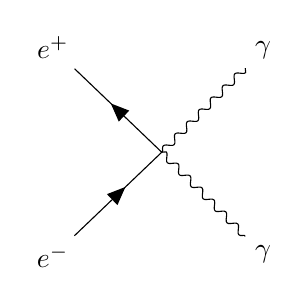
\begin{tikzpicture}
\begin{feynman}
\vertex (c) ;
\vertex [below left =of c] (i1){\(e^{-}\)};
\vertex [above left=of c] (i2) {\(e^{+}\)};
\vertex [below right=of c] (f1){\(\gamma\)};
\vertex [above right= of c] (f2){\(\gamma\)};
\diagram* {
(i1) -- [fermion] (c) -- [fermion] (i2) ,
(f1) -- [photon] (c)-- [photon] (f2)
};
\end{feynman}
\end{tikzpicture}
\caption{Electron-Positron Annihilation}
\label{Fey:e-p}
\end{center}
\end{figure}

\indent The weak interaction defines the interaction of particles under the weak isospin quantum number. There are two copies of each of every fermion, a left and a right-handed chirality version. Particle with a right-handed chirality have a weak isospin T = 0. These particles exist as singlets and do not interact with the weak force. Left-handed particles have a weak isospin T =  ${\frac{1}{2}}$. These particles live as doublets as illustrated in table ~\ref{tab:chiral}. For these particles, the third component of the weak isospin T\textsubscript{3}, ${+\frac{1}{2}}$ for up-type quarks and charged leptons and ${-\frac{1}{2}}$ for down-type quarks and neutral leptons. Under weak interactions, particles with ${T_{3} = +\frac{1}{2}}$ always transform into particles with ${T_{3} = -\frac{1}{2}}$, or vice versa.\linebreak

\begin{table}[h]
\begin{center}
\def\arraystretch{1.5}
\begin{tabular}[h]{|c|c|}
\hline
Left Handed Fermions, ${T = \frac{1}{2}, T_{3} = \pm\frac{1}{2}}$ & Right Handed Fermions, ${T = 0, T_{3} = 0}$\\
\hline\hline
${\binom{u}{d}}$, ${\binom{c}{s}}$, ${\binom{t}{b}}$, ${\binom{e}{\nu_{e}}}$, ${\binom{\mu}{\nu_{\mu}}}$, ${\binom{\tau}{\nu_{\tau}}}$ & u, d, c, s, t, b, e, ${\nu_{e}}$, ${\mu}$, ${\nu_{\mu}}$, ${\tau}$, ${\nu_{\tau}}$ \\
\hline
\end{tabular}
\caption{Particles of the Standard Model (ref XXX (ian or PDG))}
\label{tab:chiral}
\end{center}
\end{table}


 \indent The remaining piece of the weak interaction is the W boson. The W has an isospin of T = 1. This gives three option for the third component of isospin, ${T_{3} = +1, 0, -1}$ which give the W\textsuperscript{+}, the W\textsuperscript{0}, and the W\textsuperscript{-}. W\textsuperscript{0} will be discussed more in ~\ref{ssec:Higgs}. The ${W^{\pm}}$ either raise or lower the ${T_{3}}$ of the fermions. ~\ref{Fig:weak_dia} is an example of a weak interaction.\linebreak

\begin{figure}[h]
\begin{center}

\begin{tikzpicture}
\begin{feynman}
\vertex (i1){\(e^{-}\)};
\vertex [right =of i1] (c);
\vertex [right=of c] (f1) {\(\nu_{e}\)};
\vertex [below right=of c] (f2){\(W^{-}\)};
\diagram* {
(i1) -- [fermion] (c),
(f2) -- [boson] (c)-- [fermion] (f1)
};
\end{feynman}
\end{tikzpicture}
\caption{electron emitting an electron neutrino and a W Boson}
\label{Fig:weak_dia}
\end{center}
\end{figure}

%Here, write about mixing and electroweak interaction?
%Also need to talk briefly about QCD
%Need to talk about b-quarks specifically.

%\begin{equation}
%Y_{W} = 2(Q - T_{3})
%\end{equation}


\indent %Need to talk about couplings and decays more in depth here
\subsection{The Higgs Mechanism and Higgs Boson}
\label{ssec:Higgs}
%Start with need massless gauge bosons to fufill local gauge invariance. So we have W 1,2,3, and b. explain the mixing and the  break the symmetry to give the W+- Z and photon. Give math to explain this?? Show how this gives rise to a new boson, the higgs. 
QED is a gauge invariant theory. This means the Lagrangian that describes the system is invariant under local gauge transformations. For the electroweak theory, this is the electroweak symmetry. To satisfy this symmetry, the bosons must be massless. However, the electroweak bosons in the standard model, the ${W^{\pm}}$ the ${Z}$ and the ${\gamma}$ are not all massless. This means that the electroweak symmetry must be broken by something.\linebreak

\begin{figure}[h]
\begin{center}
\includegraphics[scale=0.65]{figures/higgspotential}
\caption{The Higgs potential (from http://cds.cern.ch/record/1638469/plots) }
\label{Fig:higgspot}
\end{center}
\end{figure}

\indent In QED, the five gauge bosons are ${W^{i}_{\mu}, i = 1,2,3}$ and ${B_{\mu}}$. These bosons couple to a complex scalar Higgs doublet, ${\Phi \equiv \binom{\phi^{+}}{\phi^{0}}}$. This doublet has a scalar potential.
\begin{equation}
V(\Phi) = \mu^{2}|\Phi^{\dagger}\Phi| + \lambda(|\Phi^{\dagger}\Phi|)^{2}
\end{equation}
Where ${\mu^{2} < 0}$. This gives the Mexican hat shaped potential seen in figure ~\ref{Fig:higgspot}, with a minimum energy at 
\begin{equation}
\langle \phi \rangle = \sqrt{-\frac{\mu^{2}}{2\lambda}}\equiv \frac{\nu}{\sqrt{2}}
\end{equation}
called the vacuum expectation value (VEV) of ${\phi}$. The choice of the direction of fluctuation is arbitrary but can be chosen such that


 
\begin{equation}
\phi_{0} = \frac{1}{\sqrt{2}} \binom{0}{\nu}
\end{equation}
After the direction is chosen and the only remaining piece is the scalar field h(x), giving 
\begin{equation}
\phi(x) = \phi_{0} + h(x)
\end{equation}
The doublet can now be described by 
\begin{equation}
\Phi = \frac{1}{sqrt{2}} \binom{0}{v+h(x)}
\end{equation}
The Higgs field couples to the gauge bosons as 
\begin{equation}
(\frac{g}{2}\overrightarrow{\tau}\cdot \overrightarrow{W} + \frac{g'}{2}B)\phi_{0}
\end{equation}
Where ${\overrightarrow{\tau}}$ are the Pauli matrices, ${\overrightarrow{W}}$ are ${W_{1,2,3}}$ and g, g' are the coupling constants. The result of the coupling is the acquisition of mass by three eigenstates of the bosons, 
\begin{equation}
\begin{split}
W^{\pm} = \frac{1}{\sqrt{2}}(W^{1}_{\mu} \mp iW^{2}_{\mu})\\
Z^{\mu} = \frac{-g'B_{\mu} + gW^{3}_{\mu}}{\sqrt{g^{2} + g'^{2}}}\\
A^{\mu} = \frac{gB_{\mu} + g'W^{3}_{\mu}}{\sqrt{g^{2} + g'^{2}}}
\end{split}
\end{equation}
These four eigenstates are the bosons we observe in the standard model. With Masses
\begin{equation}
\begin{split}
M^{2}_{W} = \frac{1}{4}g^{2}\nu^{2} \\
M^{2}_{Z} = \frac{1}{4}(g^{2} + g'^{2})\nu^{2} \\
M_{A} = 0
\end{split}
\end{equation}
Through the mixing that occurs in the spontaneous electroweak symmetry breaking gives mass to the standard model Gauge Bosons while leaving the photon massless. However, for this to occur, an additional scalar field, the Higgs Field, is required.\linebreak
\indent The Higgs Boson is an excitation in the scalar Higgs field predicted in 1964. The decay mechanism of this massive boson was predicted by Peter Higgs, allowing for the decay products to be measured. Giving a way to prove the existence of the scalar Higgs field. In 2012, a Higgs like scalar boson was discovered at the LHC by the ATLAS and CMS experiments with a mass of 125GeV/c\textsuperscript{2} (ref XXX https://arxiv.org/abs/1207.7214). Since the discovery, many measurements have been made of this Higgs Boson to compare it to the standard model Higgs Boson. So far, the Higgs Boson has held up to these tests. The Higgs Boson has spin-parity J\textsuperscript{P} = 0\textsuperscript{+} 
(ref XXX %https://www.sciencedirect.com/science/article/pii/S0370269313006527?via%3Dihub)
, decays to bb (https://www.sciencedirect.com/science/article/pii/S0370269318307056), ${\gamma\gamma, \tau\tau}$,(ref XXX https://arxiv.org/abs/1811.08856) WW and ZZ have been measured with appropriate signal strengths, and no significant deviations have been observed in any Run 2 analyses. However, there are still many parameters of the Higgs Boson that still need measured. One of which is the triple Higgs coupling.
%Do I want to include more about the higgs discovery. 

%%\clearpage
%%-------------------------------------------------------------------------------
%
%
%%%-------------------------------------------------------------------------------
%\input{ATLASdetector}
%%\clearpage
%%-------------------------------------------------------------------------------
%
%%%-------------------------------------------------------------------------------
%\input{TriggerData}
%%\clearpage
%%-------------------------------------------------------------------------------
%
%
%%%-------------------------------------------------------------------------------
%\input{Simulation}
%%\clearpage
%%-------------------------------------------------------------------------------
%
%
%%%-------------------------------------------------------------------------------
%\input{Reconstruction}
%%\clearpage
%%-------------------------------------------------------------------------------
%
%
%%-------------------------------------------------------------------------------
%\input{SignalRegions}
%%\clearpage
%%%-------------------------------------------------------------------------------
%
%
%%%-------------------------------------------------------------------------------
%\input{Background}
%%\clearpage
%%-------------------------------------------------------------------------------
%
%
%%%-------------------------------------------------------------------------------
%\input{Systematics}
%%\clearpage
%%-------------------------------------------------------------------------------
%
%
%%%-------------------------------------------------------------------------------
%\input{Results}
%\clearpage
%%-------------------------------------------------------------------------------
%
%%
%%% All figures and tables should appear before the summary and conclusion.
%%% The package placeins provides the macro \FloatBarrier to achieve this.
%%% \FloatBarrier
%%
%%
%%-------------------------------------------------------------------------------
%\input{Conclusions}
%%\clearpage
%%%-------------------------------------------------------------------------------
%%
%%-------------------------------------------------------------------------------
%%%-------------------------------------------------------------------------------
%%
%
%
%%The \texttt{atlaslatex} package contains the acknowledgements that were valid 
%%at the time of the release you are using.
%%These can be found in the \texttt{acknowledgements} subdirectory.
%%When your ATLAS paper or PUB/CONF note is ready to be published,
%%download the latest set of acknowledgements from:\\
%%\url{https://twiki.cern.ch/twiki/bin/view/AtlasProtected/PubComAcknowledgements}
%
%%The supporting notes for the analysis should also contain a list of contributors.
%%This information should usually be included in \texttt{mydocument-metadata.tex}.
%%The list should be printed either here or before the table of contents.
%
%
%%-------------------------------------------------------------------------------
%%\clearpage
%%\appendix
%%\part*{Appendix}
%%\addcontentsline{toc}{part}{Appendix}
%%%-------------------------------------------------------------------------------
%%
%%In a paper, an appendix is used for technical details that would otherwise disturb the flow of the paper.
%%Such an appendix should be printed before the Bibliography.
%
%
%-------------------------------------------------------------------------------
% If you use biblatex and either biber or bibtex to process the bibliography
% just say \printbibliography here

\printbibliography
%\printbibliography[title={REFERENCES CITED},heading=bibintoc]
%\bibliographystyle{atlasBibStyleWithTitle}
%\bibliography{CONF}
% If you want to use the traditional BibTeX you need to use the syntax below.
%\bibliographystyle{bibtex/bst/atlasBibStyleWoTitle}
%\bibliography{atlas-document,bibtex/bib/ATLAS}
%-------------------------------------------------------------------------------

%-------------------------------------------------------------------------------
% Print the list of contributors to the analysis
% The argument gives the fraction of the text width used for the names
%-------------------------------------------------------------------------------
%\clearpage
%\PrintAtlasContribute{0.30}

%%-------------------------------------------------------------------------------


%\clearpage


%\appendix
%\input{auxMaterial}
%\appendix
%%\part*{Auxiliary material}
%%\addcontentsline{toc}{part}{Auxiliary material}
%%-------------------------------------------------------------------------------

%In an ATLAS paper, auxiliary plots and tables that are supposed to be made public 
%should be collected in an appendix that has the title \enquote{Auxiliary material}.
%This appendix should be printed after the Bibliography.
%At the end of the paper approval procedure, this information can be split into a separate document
%-- see \texttt{atlas-auxmat.tex}.
%
%In an ATLAS note, use the appendices to include all the technical details of your work
%that are relevant for the ATLAS Collaboration only (e.g.\ dataset details, software release used).
%This information should be printed after the Bibliography.
\end{runninglinenumbers}
\end{document}
